\documentclass{report}

\usepackage{textcomp}
\usepackage{enumerate}
\usepackage{a4wide}
\usepackage{epsfig}
\usepackage{amssymb}
\usepackage{theorem}
\usepackage{fancyvrb}
\usepackage{alltt}
\usepackage{fleqn}
\usepackage{epic}
\usepackage{color}
\usepackage{wasysym}
\usepackage{hyperref}
\usepackage{soul}

\usepackage[all]{hypcap}
\hypersetup{
	colorlinks = true, % comment this to make xdvi work
	linkcolor  = blue,
	citecolor  = red,
        filecolor  = blue,
        urlcolor   = [rgb]{0.5, 0.0, 0.5},
	pdfborder  = {0 0 0} 
}
\usepackage{fancyhdr}
\usepackage{lastpage} 

\renewcommand*{\familydefault}{\sfdefault}

\pagestyle{fancy}

\fancyfoot[C]{--- \thepage/\pageref{LastPage}\ ---}

\fancypagestyle{plain}{%
\fancyhf{}
\fancyfoot[C]{--- \thepage/\pageref{LastPage}\ ---}
\renewcommand{\headrulewidth}{0pt}
}

\renewcommand{\chaptermark}[1]{\markboth{\chaptername \ \thechapter.\ #1}{}}
\renewcommand{\sectionmark}[1]{\markright{\thesection. \ #1}{}}
\fancyhead[R]{\leftmark}
\fancyhead[L]{\rightmark}


\definecolor{amethyst}{rgb}{0.2, 0.4, 0.6}
\definecolor{orange}{rgb}{1, 0.9, 0.0}

\setlength{\mathindent}{1.3cm}
\theoremstyle{plain}
\newcounter{aufgabe}
\hyphenation{Warte-schlan-ge}
\hyphenation{Ko-die-rungs}
{\theorembodyfont{\sf} \newtheorem{Definition}{Definition}}
{\theorembodyfont{\sf} \newtheorem{Notation}[Definition]{Notation}}
{\theorembodyfont{\sf} \newtheorem{Corollary}[Definition]{Corollary}}
{\theorembodyfont{\sf} \newtheorem{Lemma}[Definition]{Lemma}}
{\theorembodyfont{\sf} \newtheorem{Proposition}[Definition]{Proposition}}
{\theorembodyfont{\sf} \newtheorem{Theorem}[Definition]{Theorem}}
\title{\epsfig{file=Abbildungen/dhbw-logo.eps, scale=1.5}\\[0.3cm]  
       Algorithms  \\[0.5cm]
      --- Lecture Notes for the Summer Term 2018 ---}
\author{Prof.~Dr.~Karl Stroetmann}



% set the monospace-font to Inconsalata-g
% font-source: http://leonardo-m.livejournal.com/77079.html
\renewcommand{\encodingdefault}{T1}
\renewcommand{\ttdefault}{inconsolatag}


\date{\today\\[1.5cm]
\begin{minipage}[t]{1.0\linewidth} 
These lecture notes, their \LaTeX\ sources, and the programs discussed in these lecture notes are all available at
\\[0.2cm]
\hspace*{1.3cm}
\href{https://github.com/karlstroetmann/Algorithms}{\texttt{https://github.com/karlstroetmann/Algorithms}}.
\\[0.2cm]
The lecture notes itself can be found in the file 
\\[0.2cm]
\hspace*{1.3cm}
\href{https://github.com/karlstroetmann/Algorithms/blob/master/Lecture-Notes/algorithms.pdf}{\texttt{Lecture-Notes/algorithms.pdf}}.
\\[0.2cm]
The lecture notes are subject to continuous change.  Provided the program \href{http://git-scm.com/download}{\texttt{git}}
is installed on your computer, the repository containing the lecture notes can be cloned using the command
\\[0.2cm]
\hspace*{0.3cm}
\textcolor{amethyst}{\texttt{git clone https://github.com/karlstroetmann/Algorithms.git}}.
\\[0.2cm]
Once you have cloned the repository, the command
\\[0.2cm]
\hspace*{1.3cm}
\textcolor{amethyst}{\texttt{git pull}}
\\[0.2cm]
can be used to load the current version of these lecture notes from \href{https://github.com}{\texttt{github}}.
As these lecture notes have not yet reached their final form, I still expect some changes of these notes.
\end{minipage}
}

\newcommand{\exercise}{\vspace*{0.3cm}
  
\stepcounter{aufgabe}
\noindent
\textbf{Exercise \arabic{aufgabe}}: }

\newcommand{\proof}{
 \vspace*{0.2cm}
  
\noindent
\textbf{Proof}: }

\newcommand{\solution}{
  
\noindent
\textbf{Solution}: }

\newcommand{\example}{
\vspace*{0.2cm}
  
\noindent
\textbf{Example}: \ }

\newcommand{\examples}{

\noindent
\textbf{Examples}: \ }

\newcommand{\remark}{

\noindent
\textbf{Remark}: \ }

\newcommand{\hint}{

\noindent
\textbf{Hint}: \ }

\newcommand{\blue}[1]{{\color{blue}#1}}
\newcommand{\red}[1]{{\color{red}#1}}
\newcommand{\magenta}[1]{{\bf\color{magenta}#1}}

\newcommand{\mod}{\;\texttt{\%}\;}
\newcommand{\hoare}[3]{\bigl\{#1\bigr\}\quad\texttt{#2}\quad\bigl\{#3\bigr\}}
\newcommand{\folge}[1]{\bigl(#1\bigr)_{n\in\mathbb{N}}}
\newcommand{\bruch}[2]{{\displaystyle \frac{\displaystyle \raisebox{1pt}[0pt][-0pt]{$\,#1\,$}}{\displaystyle \raisebox{0pt}[10pt]{$\,#2\,$}}}}
\newcommand{\h}{\mathcal{H}}
\newcommand{\Oh}{\mathcal{O}}
\newcommand{\Java}{\textsl{Java}}
\newcommand{\Bin}{\mathcal{B}}
\newcommand{\AVL}{\mathcal{A}}
\newcommand{\head}{\mbox{\tt head}}
\newcommand{\tail}{\mbox{\tt tail}}
\newcommand{\conclude}{\hspace*{\fill} $\Box$}
\newcommand{\nodes}{{\mathbb V}}
\newcommand{\edges}{{\mathbb E}}
\newcommand{\paths}{{\mathbb P}}
\newcommand{\weight}[1]{\|#1\|}
\newcommand{\Weight}[1]{\bigl\|#1\bigr\|}
\newcommand{\N}{{\mathbb N}}
\newcommand{\R}{{\mathbb R}}
\newcommand{\df}{\;:=\;}
\newcommand{\ds}{\displaystyle}
\newcommand{\source}{\mbox{\tt source}}
\newcommand{\target}{\mbox{\tt target}}
\newcommand{\spath}{\mathtt{sp}}
\newcommand{\el}{\!\in\!}
\newcommand{\BT}{\mathrm{BT}}
\def\pair(#1,#2){\langle #1, #2 \rangle}
\newcommand{\qed}{\hspace*{\fill} $\Box$ \vspace*{0.2cm}}
\newcommand{\qeds}{\hspace*{\fill} $\Box$}
\newcommand{\eox}{\hspace*{\fill} $\diamond$ \vspace*{0.2cm}}
\newcommand{\eoxs}{\hspace*{\fill} $\diamond$}
\newcommand{\lb}{\hspace*{\fill} \linebreak}

\hyphenation{stra-te-gy}

\begin{document}
\maketitle
\tableofcontents
\chapter{Introduction}
\section{Motivation}
The previous lecture during the past winter term has shown us how interesting problems can be solved with the
help of sets and relations.  However, we did not discuss how \blue{sets} and \blue{relations} can be
represented by \blue{data structures} and how the operations on sets can be implemented in an efficient way.  This
course will answer these questions:  We will develop a number of different data structures that can be used to
realize both sets and relations. Furthermore, we will discuss a number of other data structures and
algorithms that should be in the toolbox of every computer scientist.

While the class in the last term has introduced the students to the theoretical foundations of
computer science, this class is more practical.  Indeed, it may be one of the most 
important classes for your future career: Five years after their students have graduated, Stanford University
regularly asks their former students to rank those classes that were the most useful for their professional
career.  Together with programming and databases, the class on algorithms consistently ranks highest.
On \href{https://quora.com}{Quora}, the answers to the question
\\[0.1cm]
\hspace*{1.3cm}
``\href{What are the 5 most important CS courses that every computer science student must take?}{
  What are the 5 most important CS courses that every computer science student must take?}''
\\[0.1cm]
consistently list the class \blue{algorithms and data structures} among those courses that are most valuable
for a professional career.  The practical importance of the topic of this class can also be seen by the
availability of book titles like
``\href{https://www.amazon.com/Algorithms-Interviews-Adnan-Aziz/dp/1453792996}{Algorithms for Interviews}''  
\cite{aziz:10} or the \href{http://www.youtube.com/watch?v=k4RRi_ntQc8}{Google job interview questions}.
 
 
\section{Overview}
This lecture covers the design and the analysis of algorithms.  We will discuss the following topics.
\begin{enumerate}
% \item Undecidability of the \href{http://en.wikipedia.org/wiki/Halting_problem}{halting problem}.

%       At the beginning of the lecture we discuss the limits of computability:  We will show that
%       there is no \textsc{SetlX} function \texttt{doesTerminate} such that for a given function $f$
%       of one argument and a string $s$ the expression
%       \\[0.2cm]
%       \hspace*{1.3cm}
%       $\texttt{doesTerminate}(f, s)$ 
%       \\[0.2cm]
%       yields \texttt{true} if the evaluation of $f(s)$ terminates and yields \texttt{false} otherwise.
\item \href{http://en.wikipedia.org/wiki/Computational_complexity_theory}{Complexity} of algorithms.

      In general, in order to solve a given problem it is not enough to develop an algorithm that
      implements a function $f$ that computes the  value $f(x)$ for a given argument $x$.  It is also important  
      that the computation of $f(x)$ does not consume too much \blue{time} and \blue{memory}.  Therefore, we want to have
      \blue{efficient} algorithms.
      In order to be able to discuss the efficiency of algorithms we have to introduce two 
      mathematical notions.
      \begin{enumerate}
      \item \href{http://en.wikipedia.org/wiki/Big_Oh}{Big O notation} offers a convenient way to
            discuss the growth rate of functions.  This notation is useful to abstract from
            unimportant details when discussing the runtime of algorithms.  
      \item The notion of a \href{http://en.wikipedia.org/wiki/Recurrence_relation}{recurrence relation}
            is the discrete analogue of the notion of a 
            \href{http://en.wikipedia.org/wiki/Differential_equation}{differential equation}.  
            Recurrence relations occur naturally when analysing the runtime of algorithms.  We present the 
            \href{https://en.wikipedia.org/wiki/Master_theorem_(analysis_of_algorithms)}{Master Theorem} that estimates
            the growth of \blue{recursive} functions.
      \end{enumerate}
\item \href{http://en.wikipedia.org/wiki/Abstract_data_types}{Abstract data types}.

      Abstract data types are a means to describe the behaviour of an algorithm in a concise way.
      Furthermore, abstract data types are part of the foundations of 
      \href{https://en.wikipedia.org/wiki/Object-oriented_programming}{object-oriented programming}. 
\item \href{http://en.wikipedia.org/wiki/Sorting_algorithm}{Sorting algorithms}.

      Sorting algorithm are among those algorithms that are most frequently used in practice.  Furthermore,
      these algorithms are easy to understand and easy to analyse.  Therefore, we start our discussion of
      algorithms and their complexity with sorting algorithms.  In this lecture, we discuss the following
      sorting algorithms: 
      \begin{enumerate}
      \item \href{http://en.wikipedia.org/wiki/Insertion_sort}{insertion sort},
      \item \href{http://en.wikipedia.org/wiki/Selection_sort}{selection sort},
      \item \href{http://en.wikipedia.org/wiki/Merge_sort}{merge sort}, 
      \item \href{http://en.wikipedia.org/wiki/Quicksort}{quicksort}, and
      \item \href{https://en.wikipedia.org/wiki/Heapsort}{heapsort}.
      \end{enumerate}
%\item \href{http://en.wikipedia.org/wiki/Hoare_logic}{Hoare logic}.
%  
%      The most important property of an algorithm is its correctness.  The \blue{Hoare calculus}
%      is a method to investigate the correctness of an algorithm.  

\item \href{http://en.wikipedia.org/wiki/Map_(computer_science)}{Associative arrays}.
  
      Associative arrays are a means to represent a function.  Most modern programming
      languages provide associative array as basic data structues.  Mathematically, an associative array is
      nothing more than a functional relation.  We discuss various data structures that can be used to
      implement associative arrays efficiently. 
\item \href{http://en.wikipedia.org/wiki/Priority_queue}{Priority queues}.
  
      Many graph theoretical algorithms use priority queues as one of their basic building blocks.
      Furthermore, priority queues have important applications in the theory of operating systems
      and in simulation.
\item \href{http://en.wikipedia.org/wiki/Graph_theory}{Graph theory}.
  
      There are many applications of graphs in computer science.  The topic of graph theory is very
      rich and can easily fill a class of its own.  Therefore, we can only cover a small subset of this topic.
      In particular, we will discuss
      \href{http://en.wikipedia.org/wiki/Dijkstra%27s_algorithm}{Dijkstra's algorithm}
      for computing the shortest path.
      Furthermore, we discuss 
      \href{https://en.wikipedia.org/wiki/Kruskal%27s_algorithm}{Kruskal's algorithm} for finding the
      \href{https://en.wikipedia.org/wiki/Minimum_spanning_tree}{minimum spanning tree} of a graph.
\item \href{http://en.wikipedia.org/wiki/Monte_Carlo_method}{Monte Carlo Method} 
 
      Many important problems either do not have an exact solution at all or the computation of an
      exact solution would be prohibitively expensive.  In these cases it is often possible to use 
      simulation in order to get an approximate solution.  As a concrete example we will show
      how certain probabilities in \href{http://en.wikipedia.org/wiki/Texas_hold_%27em}{Texas hold 'em} 
      poker can be determined approximately with the help of the \blue{Monte Carlo method}.
\end{enumerate}
The primary goal of these lectures on algorithms is not to teach as many algorithms as possible.
Instead, my goal is to enable you to think algorithmically:  At the end of these
lectures, you should have acquired the following capabilities:
\begin{enumerate}
\item You should be able to understand scientific literature describing algorithms.
\item You should have acquired the skill to develop your own algorithms and to analyse their complexity.

      Of course, developing an algorithm is a process that requires a lot of creativity on your side.  However,
      once you are acquainted with a fair number of algorithms, you should be able to develop similar
      algorithms on your own. 
\end{enumerate}


\section{Algorithms and Programs}
This is a lecture on \blue{algorithms}, not on \blue{programming}.  It is important that you do not mix up
these two concepts.  An algorithm is an \blue{abstract concept} to solve a given problem.  In
contrast, a program is a \blue{concrete implementation} of an algorithm.  In order to implement an
algorithm by a program we have to cover every detail, be it trivial or not.  On the other hand, 
to specify an algorithm it is often sufficient to describe the interesting aspects.  It is
quite possible for an algorithm to leave a number of questions open.

In the literature, algorithms are usually presented as \blue{pseudo code}.  Syntactically, pseudo code looks
similar to a program, but in contrast to a program, pseudo code can also contain parts that are only
described in natural language.   However, it is important to realize that a piece of pseudo code is
\underline{not} an algorithm but is only a \blue{representation} of an algorithm.  However, the
advantage of pseudo code is that we are not confined by the arbitrariness of the syntax of a
programming language.

Conceptually, the difference between an algorithm and a program is similar to the difference between
a \blue{philosophical idea} and a \blue{text} that describes the idea.  If you have an philosophical idea, you
can write it down to make it concrete.  As you can write down the idea in English, or French or, preferably, in
ancient Greek, the textual descriptions of the idea might be quite different.  This is the same with an algorithm:
We can code it in \href{https://en.wikipedia.org/wiki/Java_(programming_language)}{Java}, or
\href{http://python.org}{Python}, or, preferably, \href{http://setlx.randoom.org}{\textsc{SetlX}}.  The
programs will be very different, but the algorithm will be the same. 

Having discussed the difference between algorithms and programs, let us now decide how to present
algorithms in this lecture.  
\begin{enumerate}
\item We can describe algorithms using natural language.  While natural language certainly is
      expressive enough, it also suffers from ambiguities.  Furthermore, natural language
      descriptions of complex algorithms tend to be difficult to follow.
\item Instead, we can describe an algorithm by implementing it.  There is certainly no ambiguity
      in a program, but on the other hand this approach would require us to implement every aspect
      of an  algorithm and our descriptions of algorithms would therefore get longer than we want.
\item Finally, we can try to describe algorithms in the language of mathematics.  This language is 
      concise, unambiguous, and easy to understand, once you are accustomed to it.  This is
      therefore our method of choice.

      However, after having presented an algorithm in the language of mathematics, it is often very
      simple to implement this algorithm in the programming language
      \href{http://randoom.org/Software/SetlX}{\textsc{SetlX}}.  The reason is 
      that \textsc{SetlX} is based on set theory, which is the language of mathematics.  We will see
      that \textsc{SetlX} enables us to present and implement algorithms on a very high abstraction level.
\end{enumerate}

\section{Desirable Properties of Algorithms}
Before we start with our discussion of algorithms we should think about our goals when designing
algorithms.  
\begin{enumerate}
\item Algorithms have to be \blue{correct}.
\item Algorithms should be \blue{efficient} with respect to both \blue{computing time} and \blue{memory}.
\item Algorithms should be \blue{simple}.
\end{enumerate}
The first goal in this list is so self-evident that it is often overlooked.  The
importance of the last goal might not be as obvious as the other goals.
However, the reason for the last goal is economical:  If it takes too long to code an algorithm, the
cost of the implementation might well be unaffordable.  Furthermore, even if the budget is next to unlimited,
there is another reasons to strife for simple algorithms:  If the conceptual complexity of an algorithm is too
high, it may become impossible to check the correctness of the implementation.  Therefore, the third goal is
strongly related to the first goal.  

\section{Literature}
These lecture notes are intended to be the main source for my lecture.  Additionally, I want
to mention those books that have inspired me most.
\begin{enumerate}
\item \textsl{Robert Sedgewick}: \href{https://www.amazon.com/Algorithms-4th-Robert-Sedgewick/dp/032157351X}{Algorithms}, 
      fourth edition, Pearson, 2011, \cite{sedgewick:11}.
    
      This book has a nice \href{http://algs4.cs.princeton.edu/home/}{booksite} containing a wealth
      of additional material.  This book seems to be the best choice for the working practitioner.
      Furthermore, \href{http://www.cs.princeton.edu/~rs/}{Professor Sedgewick} teaches an excellent 
      \href{https://www.coursera.org/course/algs4partI}{course} on algorithms that is available at
      \href{https://www.coursera.org/}{coursera.org}.  This course is based on this book.  Furthermore, all
      the algorithms discussed in this book are implemented in \textsl{Java}, so reading this book
      also strengthens your knowledge of \textsl{Java}.
\item \textsl{Alfred V.~Aho}, \textsl{John E.~Hopcraft}, and \textsl{Jeffrey D.~Ullman}:
      \blue{Data Structures and Algorithms}, Addison-Wesley, 1987, \cite{aho:87}.
      
      This book is a bit dated now but it is one of the classics on algorithms.  It discusses algorithms at an
      advanced level.
\item \textsl{Thomas H.~Cormen}, \textsl{Charles E.~Leiserson}, 
      \textsl{Ronald L.~Rivest}, and \textsl{Clifford Stein}:
      \href{https://www.amazon.com/Introduction-Algorithms-3rd-MIT-Press/dp/0262033844}{Introduction to Algorithms}, 
      third edition, MIT Press, 2009, \cite{cormen:09}

      Due to the level of detail and the number of algorithms given, this
      \href{https://en.wikipedia.org/wiki/Introduction_to_Algorithms}{book} can be viewed as a reference work. 
      This book requires more mathematical sophistication on the side of its readers than any of the
      other books referenced here.  
\item \blue{Einf�hrung in die Informatik},
      written by \textsl{Heinz-Peter Gumm} and \texttt{Manfred Sommer} \cite{gumm:2013}.
      
      This German book is a very readable introduction to computer science and it has a chapter
      on algorithms that is fairly comprehensive.  Furthermore, this book is
      \blue{available} electronically in our \href{http://www.bib.dhbw-mannheim.de}{library}. 
\item Furthermore, there is a set of outstanding 
      \href{https://class.coursera.org/algo-004/class/index}{video lectures} 
      from \href{http://theory.stanford.edu/~tim/}{Professor Roughgarden}
      available at \href{https://www.coursera.org/}{coursera.org}.
\end{enumerate}


\section{A Final Remark}
There is one final remark I would like to make at this point:  Frequently, I get questions from
students concerning the exams.  While I will most gladly answer these questions, I should warn you
that, 50\%  
of the time, my answers will be flat out lies.  The other 50\%,
my answers will be some random rubbish.  Please bear that in mind when evaluating my answers.

\section{A Request}
Computer science is a very active field of research.  Furthermore, my comprehension of the English
language is improving steadily.  Therefore, these lecture notes are constantly
evolving and hence might contain typos or even mistakes.  If you find a problem,
please take the time and either send me an email or a message on discord.  My email address is
\\[0.2cm]
\hspace*{1.3cm}
\href{mailto:karl.stroetmann@dhbw-mannheim.de}{karl.stroetmann@dhbw-mannheim.de}.
\\[0.2cm]
If you are familiar with \href{http://github.com}{\texttt{github}}, you might even consider
sending me a \href{https://help.github.com/articles/using-pull-requests}{pull request}.

Finally, if you have any questions regarding the material presented in this course, you are
welcome to ask questions either by \href{mailto:karl.stroetmann@dhbw-mannheim.de}{email},
\href{https://discordapp.com}{discord}.  If you think that others might
have the same question, it is best if you ask your question via discord.
All your questions are welcome since they give me valuable feedback how 
\red{\st{stupid you really are}} to improve my lecture. 


%%% local Variables: 
%%% mode: latex
%%% TeX-master: "algorithms"
%%% End: 

%\include{limits}
\chapter{Big $\mathcal{O}$ Notation} 
This chapter introduces both the
\href{http://en.wikipedia.org/wiki/O_notation}{big $O$ notation} and the
\blue{tilde notation} advocated by Sedgewick \cite{sedgewick:11}.
These two notions are needed to analyse the running time of algorithms.  In order to illustrate
the application of these notions, we show how to implement the computation of powers efficiently,
i.e.~we discuss how to evaluate the expression $a^b$ for given $a,b \in \mathbb{N}$ in a way that
is significantly faster than the naive approach. 

\section{Motivation}
Sometimes it is necessary to have a precise understanding of the complexity of an algorithm.  
In order to obtain this understanding we could proceed as follows:  
\begin{enumerate}
\item We implement the algorithm in a given programming language.
\item We count how many additions, multiplications, assignments, etc.~are needed
      for an input of a given length.
\item We read the processor handbook to look up the amount of time that is needed for the different operations.
\item Using the information discovered in the previous two steps we can then predict the running
      time of our algorithm for given input.
\end{enumerate}
This approach is problematic for a number of reasons.
\begin{enumerate}
\item It is very complicated.
\item The execution time of the basic operations is highly dependent on the memory hierarchy of the
      computer system:  For many modern computer architectures, adding two numbers that happen to be
      in a \blue{register} is more than ten times faster than adding two numbers that reside in
      \blue{main memory}.  Unless we peek into the machine code generated by our compiler, it is very difficult
      to predict whether a variable will be stored in memory or in a register.  Even if a variable
      is stored in main memory, we still might get lucky if the variable is also stored in a \blue{cache}.
\item If we would later code the algorithm in a different programming language or if we would port
      the program to a computer with a different processor we would have to redo most of the
      computation. 
\end{enumerate}
The final reason shows that the approach sketched above is not well suited to measure the complexity of
an algorithm: After all, the notion of an algorithm is more abstract than the notion of a program
and we really need a notion measuring the complexity of an algorithm that is more abstract than the
notion of the running time of a program.  This notion of complexity should satisfy the following
specification: 
\begin{itemize}
\item The notion of complexity should \blue{abstract from constant factors}.  After all, according to 
      \href{http://en.wikipedia.org/wiki/Moore's_law}{Moore's law}, 
      computers hitting the market 18 month from now will be about twice as powerful as today's computers.

\item The notion should abstract from \blue{insignificant terms}.

      Assume you have written a program that  multiplies two $n \times n$ matrices.  Assume,
      furthermore, that you have computed the running time $T(n)$ of this program as a function 
      of the size $n$ of the matrix as
      \\[0.2cm]
      \hspace*{1.3cm} $T(n) = 3 \cdot n^3 + 2 \cdot n^2 + 7$. 
      \\[0.2cm]
      When compared with the total running time, the portion of running time that is due to the term 
      $2\cdot n^2 + 7$ will decrease with increasing value of $n$.  To see this, consider the
      following table:
      \\[0.3cm]
      \hspace*{1.3cm} 
      \begin{tabular}{|r|r|}
        \hline
        $n$  & \rule{0pt}{16pt} $\bruch{2 \cdot n^2 + 7}{3 \cdot n^3 + 2 \cdot n^2 + 7}$ \\[0.3cm]
        \hline
        \hline
        1       &  0.75000000000000  \\
        10      &  0.06454630495800  \\
        100     &  0.00662481908150  \\
        1000    &  0.00066622484855  \\
        10\,000 &  6.6662224852\,e\,-05  \\
       \hline
      \end{tabular}

      This table clearly shows that, for large values of $n$, the term $2 \cdot n^2 + 7$ can be
      neglected. 
\item The notion of complexity should describe how the running time increases
      when the size of the input increases:  For small inputs, the running time is not very
      important but the question is how the running time \blue{grows} when the size of the input is increased. 
      Therefore the notion of complexity should capture the relation between the input size and the running time.
\end{itemize}
Let us denote the set of all positive real numbers\footnote{
  In the literature, the set of positive real numbers is usually denoted as $\mathbb{R}_{>0}$.  I prefer the
  notation $\mathbb{R_+}$ because it is shorter.
}
as $\R_+$, i.e.~let us define 
\\[0.2cm]
\hspace*{1.3cm}
$\R_+ := \{ x \in \R \mid x > 0 \}$. 
\\[0.2cm]
Furthermore, the set of all functions defined on  $\N$ yielding a positive real number is defined
as: 
\\[0.2cm]
\hspace*{1.3cm} 
$\R_+^{\;\N} = \bigl\{ f \mid \mbox{$f$ is a function of the form $f: \N \rightarrow \R_+$} \}$.

\begin{Definition}[$\Oh(g)$] 
Assume $g \in \R_+^{\N}$ is given.   Let us define the set of all functions that \blue{grow at most as fast}
  as the function $g$ as follows:
  \\[0.2cm]
  \hspace*{0.5cm} 
  \colorbox{red}{\framebox{\colorbox{orange}{
  $ \Oh(g) \;:=\; \left\{ f \in \R_+^{\;\N} \mid \exists k \in \N \colon 
    \exists c \in \R_+\colon \forall n \in \N \colon \bigl(n \geq k \rightarrow f(n) \leq c \cdot g(n)\bigr) \right\}$.}}}
  \eox
\end{Definition}

The definition of $\Oh(g)$ contains three nested quantifiers and may be difficult to understand
when first encountered.  Therefore, let us analyse this definition carefully.  Let us consider a
function $g \in \R_+^\N$.  Informally, $f \in \Oh(g)$ is true if the function $f$ does not grow faster than
the function $g$.  
\begin{enumerate}
\item The fact that $f \in \Oh(g)$ holds does not impose any restriction on small values of $n$.
      After all, the condition
      \\[0.2cm]
      \hspace*{1.3cm}
      $f(n) \leq c \cdot g(n)$
      \\[0.2cm]
      is only required for those values of $n$ that are bigger than or equal to $k$ and the value
      $k$ can be \underline{an}y\hspace*{-0.1cm}\underline{\ } suitable natural number.

      This property shows that the big $\Oh$ notation captures the \colorbox{orange}{\blue{growth rate}} of functions.
\item Furthermore, $f(n)$ can be bigger than $g(n)$ even for arbitrary values of $n$ 
      but it can only be bigger by a constant factor:  There must be some fixed constant $c$
      such that 
      \\[0.2cm]
      \hspace*{1.3cm}
      $f(n) \leq c \cdot g(n)$
      \\[0.2cm]
      holds for all values of $n$ that are sufficiently big.  This implies that if $f \in \Oh(g)$
      holds. then, for example, the function $2 \cdot f$ will also be in $\Oh(g)$.

      This last property shows that the big $\Oh$ notation \colorbox{orange}{\blue{abstracts from constant factors}}.
\end{enumerate}
I have borrowed Figure \ref{fig:big-o.eps} below from the \href{http://www.wikipedia.org}{Wikipedia} article on 
\href{http://en.wikipedia.org/wiki/Asymptotic_notation}{asymptotic notation}.  It shows two functions 
$f(x)$ and $c \cdot g(x)$ such that $f \in \Oh(g)$.  Note that the function $f(x)$, which is drawn
in red, is less or equal than $c \cdot g(x)$ for all values of $x$ such that $x \geq k$.  In the
figure, we have $k=5$, since the condition $f(x) \leq g(x)$ is satisfied for $x \geq 5$. For
values of $x$ that are less than $k = 5$, sometimes $f(x)$ is bigger than $c \cdot g(x)$ but that does
not matter.  In Figure \ref{fig:big-o.eps} the functions $f(x)$ and $g(x)$ are drawn as if they were
functions defined for all positive real numbers.  However, this is only done to support the
visualization of these functions.  In reality, the functions $f$ and $g$ are only defined for
natural numbers.


\begin{figure}[!ht]
  \centering
  \framebox{\epsfig{file=Abbildungen/big-o.eps, scale=0.50}} 
  \caption{Example for $f \in \Oh(g)$.}
  \label{fig:big-o.eps}
\end{figure}


\noindent
We discuss some concrete examples in order to further clarify the notion $f \in \Oh(g)$.

\example
We claim that the following holds:
\\[0.2cm]
\hspace*{1.3cm}
$3 \cdot n^3 + 2 \cdot n^2 + 7 \in \Oh(n^3)$. 
\\[0.2cm]
\textbf{Proof}:  We have to  provide a constant $c$ and another constant $k$ such that for all $n\in
\N$ satisfying
$n \geq k$ the inequality
\\[0.2cm]
\hspace*{1.3cm} 
$3 \cdot n^3 + 2 \cdot n^2 + 7 \leq c \cdot n^3$
\\[0.2cm]
holds.  Let us define  $k := 1$ and $c := 12$.  Then we may assume that 
\begin{equation}
  \label{eq:u1}
  1\leq n  
\end{equation}
holds and we have to show that this implies 
\begin{equation}
  \label{eq:u2}
  3 \cdot n^3 + 2 \cdot n^2 + 7 \leq 12 \cdot n^3.
\end{equation}
If we take the third power of both sides of the inequality (\ref{eq:u1}) then we see that
\begin{equation}
  \label{eq:u3pre}
  1 \leq n^3  
\end{equation}
holds.  Let us multiply both sides of this inequality with $7$.  We get: 
\begin{equation}
  \label{eq:u3}
  7 \leq 7 \cdot n^3
\end{equation}
Furthermore, let us multiply the inequality (\ref{eq:u1}) with the term $2\cdot n^2$.  This yields
\begin{equation}
  \label{eq:u4}
  2 \cdot n^2 \leq 2 \cdot n^3  
\end{equation}
Finally, we obviously have
\begin{equation}
  \label{eq:u5}
  3 \cdot n^3 \leq 3 \cdot n^3
\end{equation}
Adding up the inequalities (\ref{eq:u3}), (\ref{eq:u4}), and (\ref{eq:u5}) gives \\[0.2cm]
\hspace*{1.3cm} $3 \cdot n^3 + 2 \cdot n^2 + 7 \leq 12 \cdot n^3$ \\[0.2cm]
and therefore the proof is complete. \qed

\example
We have  $n \in \Oh(2^n)$. 

\proof
We have to provide a constant $c$ and a constant $k$
such that 
\\[0.2cm]
\hspace*{1.3cm}
$ n \leq c \cdot 2^n$ 
\\[0.2cm]
holds for all $n \geq k$.  Let us define $k := 0$ and $c := 1$.  We will then have to show that \\[0.2cm]
\hspace*{1.3cm} $n \leq 2^n$ \quad holds for all $n \in \N$.
\\[0.2cm]
We prove this claim by induction on $n$.
\begin{enumerate}
\item \textbf{Base case}: $n = 0$

      Obviously, $n = 0 \leq 1 = 2^0 = 2^n$ holds.  
\item \textbf{Induction step}: $n \mapsto n + 1$

      By the induction hypothesis we have 
      \\[0.2cm]
      \hspace*{1.3cm}
      $n \leq 2^n$.    
      \\[0.2cm]
      Furthermore, a trivial induction shows that
      \\[0.2cm]
      \hspace*{1.3cm}
      $1 \leq 2^n$.
      \\[0.2cm]
      Adding these two inequalities yields
      \\[0.2cm]
      \hspace*{1.3cm} $n+1 \leq 2^n + 2^n = 2^{n+1}$. \qed
\end{enumerate}

\exercise
\begin{enumerate}[(a)]
\item Prove that $n^2 \in \Oh(2^n)$. 
\item Prove that $n^3 \in \Oh(2^n)$. 
\item Prove that for every $\alpha \in \mathbb{N}$ we have  $n^\alpha \in \Oh(2^n)$. 
      
      \hint
      \begin{enumerate}[1.]
      \item Try to prove the following claim by induction on $\alpha$:  For every $\alpha \in \mathbb{N}$
            there exists a number $c(\alpha)$ such that
            \\[0.2cm]
            \hspace*{1.3cm}
            $n^\alpha \leq c(\alpha) \cdot 2^n$ \quad holds for all $n \in \mathbb{N}$.
            \\[0.2cm]
            In the induction step you will have to prove that there is a number $c(\alpha+1)$ such that
            \\[0.2cm]
            \hspace*{1.3cm}
            $n^{\alpha+1} \leq c(\alpha+1) \cdot 2^n$ \hspace*{\fill} $(*)$
            \\[0.2cm]
            holds.  When proving this claim you may assume by induction hypothesis that for all 
            $k \leq \alpha+1$ we have numbers $c(k)$ such that
            \\[0.2cm]
            \hspace*{1.3cm}
            $n^{k} \leq c(k) \cdot 2^n$ \quad holds for all $n \in \mathbb{N}$.
            \\[0.2cm]
            You can prove the claim $(*)$ via a side induction on $n$.
      \item The \href{https://en.wikipedia.org/wiki/Binomial_theorem}{binomial theorem} tells
            us that for all $n \in \mathbb{N}$ and all $a,b \in \mathbb{R}$ the equation
            \\[0.2cm]
            \hspace*{1.3cm}
            $\ds (a+b)^n = \sum\limits_{k=0}^n {n \choose k} \cdot a^k \cdot b^{n-k}$
            \\[0.2cm]
            holds.  Here, the expression ${n \choose k}$ is read as \blue{$n$ choose $k$} and is
            defined for all $n \in \mathbb{N}$ and all $k \in \{0, 1, 2, \cdots, n\}$ via
            \\[0.2cm]
            \hspace*{1.3cm}
            $\ds {n \choose k} = \frac{n!}{k! \cdot (n-k)!}$.
            \\[0.2cm]
            The binomial theorem should be used to expand the term $(n+1)^{\alpha + 1}$ that occurs
            in the induction step of the side induction.  \eox
      \end{enumerate}
\end{enumerate}



It would be very tedious if we would have to use induction every time we need to prove that 
$f \in \Oh(g)$ holds for some functions $f$ and $g$.   Therefore, we show a number of properties of
the big $\Oh$ notation next.  These properties will later enable us to prove a claim of the form 
$f \in \Oh(g)$ much quicker than by induction.



\begin{Proposition}[Reflexivity]
  For all functions $f\colon \N \rightarrow {\R_+}$ we have that
  \\[0.2cm]
  \hspace*{1.3cm} $f \in \Oh(f)$ \quad holds. 
\end{Proposition}

\proof
Let us define $k:=0$ and $c:=1$.  Then our claim  follows immediately from the inequality 
\\[0.2cm]
\hspace*{1.3cm}
$\forall n \in \N\colon f(n) \leq f(n)$. \qed

\begin{Proposition}[Multiplication with Constants] \hspace*{\fill} \linebreak
Assume that we have functions  $f,g\colon \N \rightarrow {\R_+}$ and a number $d \in \R_+$.  Then we
have 
\\[0.2cm]
\hspace*{1.3cm}
 $g \in \Oh(f) \rightarrow d \cdot g \in \Oh(f)$.
\end{Proposition}

\proof
The premiss $g \in \Oh(f)$ implies that there are constants $c'\in \R_+$ and $k'\in \N$ 
such that \\[0.2cm]
\hspace*{1.3cm} 
$\forall n \in \N \colon \bigl(n \geq k'  \rightarrow g(n) \leq c' \cdot f(n)\bigr)$ 
\\[0.2cm]
holds.  If we multiply the inequality involving $g(n)$ with $d$, we get \\[0.2cm]
\hspace*{1.3cm} 
$\forall n \in \N \colon\bigl( n \geq k'  \rightarrow d \cdot g(n) \leq d \cdot c' \cdot f(n)\bigr)$ 
\\[0.2cm]
Let us therefore define $k:=k'$ and $c := d \cdot c'$.  Then we have \\[0.2cm]
\hspace*{1.3cm}
$\forall n \in \N \colon \bigl(n \geq k  \rightarrow d \cdot g(n) \leq c \cdot f(n)\bigr)$ 
\\[0.2cm]
and by definition this implies $d \cdot g \in \Oh(f)$. \qed
\vspace*{0.2cm}

\remark 
The previous proposition shows that the big $\Oh$ notation does indeed abstract
from constant factors. \eox

\begin{Proposition}[Addition]
Assume that $f,g,h \colon \N \rightarrow {\R_+}$. Then we have 
\\[0.2cm]
\hspace*{1.3cm}
$f \in \Oh(h) \wedge g \in \Oh(h) \,\rightarrow\, f + g \in \Oh(h)$.
\end{Proposition}

\proof
The preconditions $f \in \Oh(h)$ and $g \in \Oh(h)$ imply that there are constants $k_1,k_2\in \N$
and $c_1,c_2\in \R$ such that both \\[0.2cm]
\hspace*{1.3cm} 
$\forall n \in \N \colon \bigl( n \geq k_1 \rightarrow f(n) \leq c_1 \cdot h(n)\bigr)$ 
\quad and
\\[0.2cm]
\hspace*{1.3cm} 
$\forall n \in \N \colon\bigl( n \geq k_2 \rightarrow g(n) \leq c_2 \cdot h(n)\bigr)$
\\[0.2cm]
holds.  Let us define $k := \max(k_1,k_2)$ and $c:= c_1 + c_2$.  For all $n \in \mathbb{N}$ such
that $n \geq k$ it then follows that both
\\[0.2cm]
\hspace*{1.3cm}
 $f(n) \leq c_1 \cdot h(n)$ \quad and \quad  $g(n) \leq c_2 \cdot h(n)$
\\[0.2cm]
holds.  Adding these inequalities we conclude that 
\\[0.2cm]
\hspace*{1.3cm} $f(n) + g(n) \leq (c_1 + c_2) \cdot h(n) = c \cdot h(n)$
\\[0.2cm]
holds for all $n \geq k$.
\qed

\exercise
Assume that $f_1,f_2,h_1,h_2 \colon \N \rightarrow {\R_+}$.  Prove that 
\\[0.2cm]
\hspace*{1.3cm}
$f_1 \in \Oh(h_1) \wedge f_2 \in \Oh(h_2) \,\rightarrow\, f_1 \cdot f_2 \in \Oh(h_1 \cdot h_2)$
\quad holds.  \eox


\exercise
Assume that $f_1,f_2,h_1,h_2 \colon \N \rightarrow {\R_+}$.  Prove or refute the claim that 
\\[0.2cm]
\hspace*{1.3cm}
$f_1 \in \Oh(h_1) \wedge f_2 \in \Oh(h_2) \,\rightarrow\, f_1 / f_2 \in \Oh(h_1 / h_2)$
\quad holds.  \eox

\begin{Proposition}[Transitivity]
Assume $f,g,h \colon \N \rightarrow {\R_+}$. Then we have \\[0.2cm]
\hspace*{1.3cm}
 $f \in \Oh(g) \wedge g \in \Oh(h) \,\rightarrow\, f \in \Oh(h)$.

\end{Proposition}

\proof
The precondition $f \in \Oh(g)$ implies that there exists a $k_1 \in \N$ and a number $c_1 \in \R$
such that 
\\[0.2cm]
\hspace*{1.3cm} 
$\forall n \in \N \colon\bigl( n \geq k_1 \rightarrow f(n) \leq c_1 \cdot g(n)\bigr)$ 
\\[0.2cm]
holds, while the precondition $g \in \Oh(h)$ implies the existence of $k_2 \in \N$ and $c_2 \in \R$
such that \\[0.2cm]
\hspace*{1.3cm} 
$\forall n \in \N \colon\bigl( n \geq k_2 \rightarrow g(n) \leq c_2 \cdot h(n)\bigr)$ 
\\[0.2cm]
holds.  Let us define $k:= \max(k_1,k_2)$ and $c := c_1 \cdot c_2$.  Then for all $n \in \mathbb{N}$
such that $n \geq k$ we have the following:
\\[0.2cm]
\hspace*{1.3cm}
$f(n) \leq c_1\cdot g(n)$ \quad and \quad $g(n) \leq c_2 \cdot h(n)$. 
\\[0.2cm]
Let us multiply the second of these inequalities with $c_1$.  Keeping the first inequality this yields
\\[0.2cm]
\hspace*{1.3cm}
$f(n) \leq c_1\cdot g(n)$  \quad and \quad $c_1\cdot g(n) \leq c_1\cdot c_2 \cdot h(n)$. 
\\[0.2cm]
However, by the transitivity of the relation $\leq$, this immediately implies $f(n) \leq c \cdot h(n)$ and our
claim has been proven.  
\qed

\begin{Proposition}[Limit Proposition] \label{limit}
  Assume that $f,g \colon \N \rightarrow {\R_+}$.   Furthermore, assume that the limit 
  \\[0.2cm]
  \hspace*{3.3cm}
 $\lim\limits_{n \rightarrow \infty} \bruch{\,f(n)\,}{g(n)}$
  \\[0.2cm]
  exists.  Then we have $f \in \Oh(g)$. 
\end{Proposition}

\proof
Define \\[0.2cm]
\hspace*{1.3cm}
$\lambda := \lim\limits_{n \rightarrow \infty} \bruch{f(n)}{g(n)}$.  
\\[0.2cm]
Since the limit exists by our assumption, we know that
\\[0.2cm]
\hspace*{1.3cm}
$\ds\forall \varepsilon \in \mathbb{R}_+:\exists k \in \mathbb{R}: \forall n \in \mathbb{N}: 
 \biggl(n \geq k \rightarrow \Bigl| \frac{f(n)}{g(n)} - \lambda \Bigr| < \varepsilon \biggr)
$.
\\[0.2cm]
Since this is valid for all positive values of $\varepsilon$, let us define $\varepsilon := 1$. 
Then there exists a number $k \in \N$ such that
for all $n\in \N$ satisfying $n \geq k$ the inequality 
\\[0.2cm]
\hspace*{1.3cm}
$\left| \bruch{f(n)}{g(n)} - \lambda \right| \leq 1$ 
\\[0.2cm]
holds.  Let us multiply this inequality with $g(n)$.  As $g(n)$ is positive, this yields
\\[0.2cm]
\hspace*{1.3cm}
$|f(n) - \lambda \cdot g(n)| \leq g(n)$. 
\\[0.2cm]
The triangle inequality $|a + b| \leq |a| + |b|$ for real numbers tells us that 
\\[0.2cm]
\hspace*{1.3cm}
$f(n) =    \bigl|f(n)\bigr|
      =    \bigl|f(n) - \lambda \cdot g(n) + \lambda \cdot g(n)\bigr|
      \leq \bigl|f(n) - \lambda \cdot g(n)\bigr| + \lambda \cdot g(n)$ 
\\[0.2cm]
holds.  Combining the previous two inequalities yields
\\[0.2cm]
\hspace*{1.3cm}
$f(n) \leq \bigl|f(n) - \lambda \cdot g(n)\bigr| + \lambda \cdot g(n)
      \leq g(n) + \lambda \cdot g(n)
       =   (1 + \lambda) \cdot g(n)
$.
\\[0.2cm]
Therefore, we define
\\[0.2cm]
\hspace*{1.3cm}
 $c := 1 +  \lambda$
\\[0.2cm] 
and have shown that $f(n) \leq c \cdot g(n)$ holds for all $n \geq k$. \qed
\vspace*{0.3cm}

\noindent
The following examples show how to put the previous propositions to good use.

\example
Assume $k \in \N$.  Then we have
\\[0.2cm]
\hspace*{1.3cm}
 $n^k \in \Oh(n^{k+1})$.

\proof
We have \\[0.2cm]
\hspace*{1.3cm} 
$\lim\limits_{n \rightarrow \infty} \bruch{n^{k}}{n^{k+1}} = \lim\limits_{n \rightarrow   \infty} \bruch{1}{n} = 0$.
\\[0.2cm]
Therefore, the claim follows from the limit proposition. 
\qeds

\example
Assume $k \in \N$ and $\lambda \in \R$ where $\lambda > 1$.  Then we have \\[0.2cm]
\hspace*{1.3cm} $n^k \in \Oh(\lambda^n)$.

\proof  We will show that 
\hspace*{1.3cm} 
\begin{equation}
  \label{eq:star}
  \lim\limits_{n \rightarrow \infty} \bruch{n^{k}}{\lambda^n} = 0  
\end{equation}
is true.  Then the claim is an immediate consequence of the limit proposition. 
According to \blue{L'H\^opital's rule}\footnote{Basically, L'H\^opital's rule states that provided the
  limit $\ds \lim\limits_{x \rightarrow \infty} \frac{f'(x)}{g'(x)}$ exists and $g'(x) \not= 0$, we have
\\
\hspace*{1.3cm}
$\ds\lim\limits_{x \rightarrow \infty} \frac{f(x)}{g(x)} = \lim\limits_{x \rightarrow \infty} \frac{f'(x)}{g'(x)}$.
\\[0.2cm]
Here $f'$ and $g'$ denote the derivatives of $f$ and $g$. 
  We will discuss L'H\^opital's rule in the lectures on analysis.
},  
the limit can be computed as follows: \\[0.2cm]
\hspace*{1.3cm} 
$\displaystyle \lim\limits_{n \rightarrow \infty} \bruch{n^{k}}{\lambda^n} =
\lim\limits_{x \rightarrow \infty} \bruch{x^{k}}{\lambda^x} =
\lim\limits_{x \rightarrow \infty} \bruch{\;\frac{\mathrm{d}x^{k}}{\mathrm{d}x}\;}{\frac{\mathrm{d}\lambda^x}{\mathrm{d}x}}$.
\\[0.2cm]
The derivatives can be computed as follows: \\[0.2cm]
\hspace*{1.3cm}
 $\displaystyle \frac{\mathrm{d}x^{k}}{\mathrm{d}x} = k \cdot x^{k-1}$ \quad and \quad 
 $\displaystyle \frac{\mathrm{d}\lambda^{x}}{\mathrm{d}x} = \ln(\lambda) \cdot \lambda^x$. \\[0.2cm]
We compute the second derivative and get \\[0.2cm]
\hspace*{1.3cm}  
$\displaystyle \frac{\mathrm{d}^{2}\,x^{k}}{\mathrm{d}x^2} = k \cdot (k-1) \cdot x^{k-2}$ \quad and \quad 
 $\displaystyle \frac{\mathrm{d}^2\,\lambda^{x}}{\mathrm{d}x^2} = \ln(\lambda)^2 \cdot \lambda^x$. \\[0.2cm]
In the same manner, we compute the $k$-th order derivative and find \\[0.2cm]
\hspace*{1.3cm} 
$\displaystyle \frac{\mathrm{d}^{k}\,x^{k}}{\mathrm{d}x^k} = k \cdot (k-1) \cdot \cdots \cdot 1 \cdot x^{0} = k!$ \quad and \quad 
 $\displaystyle \frac{\mathrm{d}^k\,\lambda^{x}}{\mathrm{d}x^k} = \ln(\lambda)^k \cdot \lambda^x$. \\[0.2cm]
After $k$ applications of L'H\^opital's rule we arrive at the following chain of equations:
\\[0.2cm]
\hspace*{1.3cm} 
$\ds 
\lim\limits_{x \rightarrow \infty} \frac{x^{k}}{\lambda^x} =
\lim\limits_{x \rightarrow \infty} \frac{\ds\;\frac{\mathrm{d}x^{k}}{\mathrm{d}x}\;}{\ds\frac{\mathrm{d}\lambda^x}{\mathrm{d}x}} =
\lim\limits_{x \rightarrow \infty} \frac{\ds\;\frac{\mathrm{d}^2\,x^{k}}{\mathrm{d}x^2}\;}{\ds\frac{\mathrm{d}^2\,\lambda^x}{\mathrm{d}x^2}} =
\cdots$
\\[0.3cm]
\hspace*{2.8cm}
$\ds = 
\lim\limits_{x \rightarrow \infty} \frac{\ds\;\frac{\mathrm{d}^k\,x^{k}}{\mathrm{d}x^k}\;}{\ds\frac{\mathrm{d}^k\,\lambda^x}{\mathrm{d}x^k}} =
\lim\limits_{x \rightarrow \infty} \frac{k!}{\ln(\lambda)^k \lambda^x} = 0$.
\\[0.2cm] 
Therefore the limit exists and the claim follows from the limit proposition.
\qed

\example
We have $\ln(n) \in \Oh(n)$.

\proof
This claim is again a simple consequence of the limit proposition.  We will use L'H\^opital's rule
to show that we have
\\[0.4cm]
\hspace*{1.3cm} 
$\lim\limits_{n \rightarrow \infty} \bruch{\;\ln(n)\;}{n} = 0$.
\\[0.2cm]
In the \href{https://github.com/karlstroetmann/Analysis/blob/master/Skript/analysis.pdf}{lecture on analysis}
it is shown that \\[0.2cm] 
\hspace*{1.3cm} $\displaystyle \frac{\mathrm{d} \ln(x)}{\mathrm{d}x} = \frac{1}{x}$ 
\quad and \quad
 $\displaystyle \frac{\mathrm{d} x}{\mathrm{d}x} = 1$. \\[0.2cm]
Therefore, we have \\[0.2cm]
\hspace*{1.3cm} 
$\displaystyle \lim\limits_{n \rightarrow \infty} \bruch{\;\ln(n)\;}{n} = 
\lim\limits_{x \rightarrow \infty} \frac{1/x}{1} = 
\lim\limits_{x \rightarrow \infty} \frac{1}{x} = 0$. \qed


\exercise
Prove that $\sqrt{n} \in \Oh(n)$ holds.  \eox

\exercise
Assume $\varepsilon \in \mathbb{R}$ and $\varepsilon > 0$.  Prove that $n \cdot \ln(n) \in \Oh\bigl(n^{1 + \varepsilon}\bigr)$
holds. \eox

\example
We have $2^n \in \Oh(3^n)$, but  $3^n \notin \Oh(2^n)$.
\eox

\proof
 First, we have \\[0.2cm]
\hspace*{1.3cm} 
$\displaystyle\lim\limits_{n \rightarrow \infty} \bruch{2^n}{3^n} = 
 \lim\limits_{n \rightarrow \infty} \left(\bruch{2}{3}\right)^n = 0$
\\[0.2cm]
and therefore we have $2^n \in \Oh\bigl(3^n\bigr)$.  The proof of $3^n \notin \Oh(2^n)$ is a 
\blue{proof by contradiction}.  Assume that 
$3^n \in \Oh(2^n)$ holds.  Then, there must be numbers $c$ and $k$ such that 
\\[0.2cm]
\hspace*{1.3cm}
$3^n \leq c \cdot 2^n$ \quad holds for $n \geq k$. 
\\[0.2cm]
Taking the logarithm of both sides of this inequality we find 
\\[0.2cm]
\hspace*{1.3cm}
$
\begin{array}{llcl}
                & \ln(3^n) & \leq & \ln(c \cdot 2^n) \\[0.2cm]
\Leftrightarrow\quad &  n \cdot \ln(3) & \leq & \ln(c) + n \cdot \ln(2) \\[0.2cm]
\Leftrightarrow &  n \cdot \bigl(\ln(3) - \ln(2)\bigr) & \leq & \ln(c)  \\[0.2cm]
\Leftrightarrow &  n  & \leq & \bruch{\ln(c)}{\ln(3) - \ln(2)}          \\[0.2cm]
\end{array}
$
\\[0.2cm]
The last inequality would have to hold for all natural numbers $n$ that are bigger than $k$.  Obviously,
this is not possible as, no matter what value $c$ takes, there are natural numbers $n$ that are bigger than 
\\[0.2cm]
\hspace*{1.3cm}
$\bruch{\ln(c)}{\ln(3) - \ln(2)}$.
\qed

\exercise
\begin{enumerate}[(a)]
\item Assume that $b > 1$.  Prove that $\log_{b}(n) \in \Oh(\ln(n))$.

      \solution
      By the definition of the natural logarithm for any positive number $n$ we have that
      \\[0.2cm]
      \hspace*{1.3cm}
      $n = \mathrm{e}^{\ln(n)}$, \quad where
      \href{http://en.wikipedia.org/wiki/E_(mathematical_constant)}{$\mathrm{e}$} denotes
      \href{https://en.wikipedia.org/wiki/Leonhard_Euler}{Euler's} number. 
      \\[0.2cm]
      Therefore, we can rewrite the expression $\log_b(n)$
      as follows:
      \\[0.2cm]
      \hspace*{1.3cm}
      $
      \begin{array}[t]{lcl}
        \log_b(n) & = & \log_b\bigl(\mathrm{e}^{\ln(n)}\bigr) \\[0.2cm]
                  & = & \ln(n) \cdot \log_b(\mathrm{e})      \\[0.2cm]
                  & = & \log_b(\mathrm{e}) \cdot \ln(n)
      \end{array}
      $
      \\[0.2cm]
      This shows that the logarithm with respect to some base $b$ and the natural logarithm 
      only differ by a constant factor, namely $\log_b(\mathrm{e})$.  Since the big $\mathcal{O}$ notation abstracts from
      constant factors, we conclude that
      \\[0.2cm]
      \hspace*{1.3cm}
      $\log_{b}(n) \in \Oh(\ln(n))$
      \\[0.2cm]
      holds. \qed

      \remark
      The previous exercise shows that, with respect to the big $\mathcal{O}$ notation, the base of
      a logarithm is not important.  The reason is that if $b > 1$ and $c > 1$ are both used as
      bases for the logarithm, we have 
      \\[0.2cm]
      \hspace*{1.3cm}
      $\log_b(n) = \log_b(\mathrm{e}) \cdot \ln(n)$ \quad and \quad $\log_c(n) = \log_c(\mathrm{e}) \cdot \ln(n)$.
      \\[0.2cm]
      Solving these equations for $\ln(n)$ yields
      \\[0.4cm]
      \hspace*{1.3cm}
      $\bruch{\log_b(n)}{\log_b(\mathrm{e})} = \ln(n)$ \quad and \quad $\bruch{\log_c(n)}{\log_c(\mathrm{e})} = \ln(n)$.
      \\[0.2cm]
      This shows that
      \\[0.4cm]
      \hspace*{1.3cm}
      $\bruch{\log_b(n)}{\log_b(\mathrm{e})} = \bruch{\log_c(n)}{\log_c(\mathrm{e})}$
      \\[0.2cm]
      holds.  This can be rewritten as
      \\[0.2cm]
      \hspace*{1.3cm}
      $\log_b(n) = \bruch{\log_b(\mathrm{e})}{\log_c(\mathrm{e})} \cdot \log_c(n)$,
      \\[0.2cm]
      showing that $\log_b(n)$ and $\log_c(n)$ differ only by a constant factor.  Therefore, we have
      \\[0.2cm]
      \hspace*{1.3cm}
      $\log_b(n) \in \Oh\bigl(\log_c(n)\bigr)$.
      \eox
\item Prove $3 \cdot n^2 + 5 \cdot n + \sqrt{n} \in \Oh(n^2)$.
\item Prove $7 \cdot n + \bigl(\log_2(n)\bigr)^2 \in \Oh(n)$.
\item Prove  $\sqrt{n} + \log_2(n) \in \Oh\left(\sqrt{n}\right)$.
\item Assume that $f, g \in \mathbb{R}_+^\mathbb{N}$ and that, furthermore, $f \in \Oh(g)$.  
      Proof or refute the claim that this implies 
      \\[0.2cm]
      \hspace*{1.3cm}
      $\displaystyle 2^{f(n)} \in \Oh\bigl(2^{g(n)}\bigr)$.
\item Assume that $f, g \in \mathbb{R}_+^\mathbb{N}$ and that, furthermore, 
      \\[0.4cm]
      \hspace*{1.3cm}
      $\lim\limits_{n \rightarrow \infty} \bruch{f(n)}{g(n)} = 0$.  
      \\[0.2cm]
      Proof or refute the claim that this implies
      \\[0.2cm]
      \hspace*{1.3cm}
      $\displaystyle 2^{f(n)} \in \Oh\bigl(2^{g(n)}\bigr)$.
\item Prove $n^n \in \mathcal{O}\bigl(2^{2^n}\bigr)$.
      \eox
\end{enumerate}

\section{A Remark on Notation}
Technically, for some function $g:\mathbb{N} \rightarrow \mathbb{R}_+$ the expression $\Oh(g)$
denotes a set.  Therefore, for a given function $f:\mathbb{N} \rightarrow \mathbb{R}_+$ we can
either have
\\[0.2cm]
\hspace*{1.3cm}
$f \in \Oh(g)$ \quad or \quad $f \not\in \Oh(g)$,
\\[0.2cm]
we can never have $f = \Oh(g)$.  Nevertheless, in the literature it has become common to abuse the
notation and write
\\[0.2cm]
\hspace*{1.3cm}
$f = \Oh(g)$ \quad instead of \quad $f \in \Oh(g)$.
\\[0.2cm]
Where convenient, we will also use this notation.  However, you have to be aware of the fact that
this is quite dangerous.  For example, if we have two different functions $f_1$ and
$f_2$ such that both
\\[0.2cm]
\hspace*{1.3cm}
$f_1 \in \Oh(g)$ \quad and \quad $f_2 \in \Oh(g)$
\\[0.2cm]
holds, when we write this as
\\[0.2cm]
\hspace*{1.3cm}
$f_1 = \Oh(g)$ \quad and \quad $f_2 = \Oh(g)$,
\\[0.2cm]
then we must not conclude that $f_1 = f_2$ as the functions $f_1$ and $f_2$ are merely members of
the same set $\Oh(g)$ and are not necessarily equal.  For example, $n \in \Oh(n)$ and 
$2 \cdot n \in \Oh(n)$,  but $n \not= 2 \cdot n$.
\vspace*{0.3cm}

Furthermore, for given functions $f$, $g$, and $h$ we write
\\[0.2cm]
\hspace*{1.3cm}
$f = g + \Oh(h)$
\\[0.2cm]
to express the fact that  $(f - g) \in \Oh(h)$.  For example, we have 
\\[0.2cm]
\hspace*{1.3cm}
$\ds n^2 + \frac{1}{2} \cdot n \cdot \log_2(n) + 3 \cdot n = n^2 + \Oh\bigl(n \cdot \log_2(n)\bigr)$.
\\[0.2cm]
This is true because
\\[0.2cm]
\hspace*{1.3cm}
$\ds\frac{1}{2} \cdot n \cdot \log_2(n) + 3 \cdot n \in \Oh\bigl(n \cdot \log_2(n)\bigr)$.
\\[0.2cm] 
The notation $f = g + \Oh(h)$ is useful because it is more precise than the pure big $\Oh$
notation.  For example, assume we have two algorithms $A$ and $B$ for sorting a list of length
$n$.  Assume further that the number $\textsl{count}_A(n)$ of comparisons used by algorithm $A$ to sort a list of
length $n$ is given as
\\[0.2cm]
\hspace*{1.3cm}
$\ds\textsl{count}_A(n) = n \cdot \log_2(n) + 7 \cdot n$,
\\[0.2cm]
while for algorithm $B$ the corresponding number of comparisons is given as
\\[0.2cm]
\hspace*{1.3cm}
$\ds\textsl{count}_B(n) = \frac{3}{2} \cdot n \cdot \log_2(n) + 4 \cdot n$.
\\[0.2cm]
Then the big $\Oh$ notation is not able to distinguish between the complexity of algorithm $A$ and
algorithm $B$ since we have
\\[0.2cm]
\hspace*{1.3cm}
$\textsl{count}_A(n) \in \Oh\bigl(n \cdot \log_2(n)\bigr)$ \quad as well as \quad
$\textsl{count}_B(n) \in \Oh\bigl(n \cdot \log_2(n)\bigr)$.
\\[0.2cm]
However, by writing
\\[0.2cm]
\hspace*{1.3cm}
$\ds\textsl{count}_A(n) = n \cdot \log_2(n) + \Oh(n)$ \quad and \quad
$\ds\textsl{count}_B(n) = \frac{3}{2} \cdot n \cdot \log_2(n) + \Oh(n)$
\\[0.2cm]
we can abstract from lower order terms while still retaining the leading coefficient of the term
determining the complexity.  

\section[Computation of Powers]{Case Study:  Efficient Computation of Powers}
Let us study an example to clarify the notions introduced so far.  
Consider the program shown in Figure \ref{fig:power-naive.stlx}.  Given an integer $m$ and a
natural number $n$, $\mathtt{power}(m, n)$ computes $m^n$.
The basic idea is to compute the value of $m^n$ according to the formula \\[0.2cm]
\hspace*{1.3cm} 
$m^n = \underbrace{m \cdot {\dots} \cdot m}_n$. 


\begin{figure}[!h]
  \centering
\begin{Verbatim}[ frame         = lines, 
                  framesep      = 0.3cm, 
                  labelposition = bottomline,
                  numbers       = left,
                  numbersep     = -0.2cm,
                  xleftmargin   = 0.8cm,
                  xrightmargin  = 0.8cm
                ]
    power := procedure(m, n) {
        r := m;
        for (i in {2 .. n}) {
            r := r * m;
        }
        return r;
    };
\end{Verbatim}
\vspace*{-0.3cm}
  \caption{Naive computation of $m^n$ for  $m,n \in \N$.}
  \label{fig:power-naive.stlx}
\end{figure} 

This program is obviously correct.  The computation of $m^n$ requires $n-1$ multiplications if the
function \texttt{power}  is implemented as shown in Figure \ref{fig:power-naive.stlx}.
Fortunately, there is an algorithm for computing $m^n$ that is much more efficient.
Consider we have to evaluate $m^4$.  We have
 \\[0.2cm]
\hspace*{1.3cm} 
$m^4 = (m \cdot m) \cdot (m \cdot m)$.
\\[0.2cm]
If the expression $m\cdot m$ is computed just once, the computation of
$m^4$ needs only two multiplications while the naive approach would already need 3 multiplications.
In order to compute $m^8$ we can proceed according to the following formula: \\[0.2cm]
\hspace*{1.3cm} 
$m^8 = \bigl( (m \cdot m) \cdot (m \cdot m) \bigr) \cdot \bigl( (m \cdot m) \cdot (m \cdot m)
\bigr)$. 
\\[0.2cm]
If the expression $(m \cdot m) \cdot (m \cdot m)$ is computed only once, then we need just 3 multiplications
in order to compute $m^8$.   On the other hand, the naive approach would take 7 multiplications to
compute $m^8$.  The general case is implemented in the program shown in Figure \ref{fig:power.stlx}.  
In this program, the value of $m^n$ is computed according to the 
\href{http://en.wikipedia.org/wiki/Divide_and_conquer_algorithm}{divide and conquer} paradigm.
The basic idea that makes this program work is captured by the following formula: 
\\[0.2cm] 
\hspace*{1.3cm} 
$m^n = 
\left\{\begin{array}{ll}
m^{n/2} \cdot m^{n/2}          & \mbox{if $n$ is even};    \\
m^{n/2} \cdot m^{n/2} \cdot m  & \mbox{if $n$ is odd}.
\end{array}
\right.
$
\vspace*{0.3cm}

\begin{figure}[!h]
  \centering
\begin{Verbatim}[ frame         = lines, 
                  framesep      = 0.3cm, 
                  labelposition = bottomline,
                  numbers       = left,
                  numbersep     = -0.2cm,
                  xleftmargin   = 0.8cm,
                  xrightmargin  = 0.8cm
                ]
    power := procedure(m, n) {
        if (n == 0) {
            return 1;
        }
        p := power(m, n \ 2);
        if (n % 2 == 0) {
            return p * p;
        } else {
            return p * p * m;
        }
    };
\end{Verbatim}
\vspace*{-0.3cm}
  \caption{Computation of $m^n$ for $m,n \in \N$.}
  \label{fig:power.stlx}
\end{figure} 

It is by no means obvious that the program shown in \ref{fig:power.stlx} does compute
$m^n$.  We prove this claim by  \blue{computational induction}.
Computational induction is an induction on the number of recursive invocations.
This method is the method of choice to prove the correctness of a recursive procedure.
The method of computational induction consists of two steps:
\begin{enumerate}
\item The \blue{base case}.

      In the base case we have to show that the procedure is correct in all those cases were it
      does not invoke itself recursively.
\item The \blue{induction step}.

      In the induction step we have to prove that the method works in all those cases were
      it does invoke itself recursively.  In order to prove the correctness of these cases we may
      assume that the recursive invocations work correctly.  This assumption is called the
      \blue{induction hypotheses}.
\end{enumerate}
Let us prove the claim 
\\[0.2cm]
\hspace*{1.3cm}
 $\mathtt{power}(m,n) = m^n$
\\[0.2cm] 
by computational induction.
\begin{enumerate}
\item \textbf{Base case}:

      The only case where \texttt{power} does not invoke itself recursively is the case $n = 0$.  
      In this case, we have
      \\[0.2cm]
      \hspace*{1.3cm} 
      $\mathtt{power}(m,0) = 1 =  m^0$.
\item \textbf{Induction step}:

      The recursive invocation of $\mathtt{power}$ has the form
      $\mathtt{power}(m,n \backslash 2)$.  By the induction hypotheses we know that 
      \\[0.2cm]
      \hspace*{1.3cm}
      $\displaystyle \mathtt{power}(m,n \backslash 2) = m^{n \backslash 2}$ 
      \\[0.2cm]
      holds.  After the recursive invocation there are two different cases:
      \begin{enumerate}
      \item $n \;\texttt{\%}\; 2 = 0$, therefore $n$ is even.

            Then there exists a number $k \in \N$ such that $n = 2 \cdot k$ and therefore
            $n / 2 = k$.
            Then, we have the following:
            \\[0.2cm]
            \hspace*{1.3cm}
           $ 
            \begin{array}{lcl}
            \mathtt{power}(m,n) & = & \mathtt{power}(m,k) \cdot \mathtt{power}(m,k) \\[0.2cm]
                                & \stackrel{IV}{=} & m^k \cdot m^k  \\[0.2cm]
                                & = & m^{2\cdot k} \\[0.2cm]
                                & = & m^{n}.
            \end{array}
            $            
      \item $n \;\texttt{\%}\; 2 = 1$, therefore $n$ is odd.

            Then there exists a number $k \in \N$ such that $n = 2 \cdot k + 1$ and we have
            $n \backslash 2 = k$, where $n \backslash 2$ denotes integer division of $n$ by $2$.
            In this case we have:
            \\[0.2cm]
            \hspace*{1.3cm}
            $ 
            \begin{array}{lcl}
            \mathtt{power}(m,n) & = & \mathtt{power}(m,k) \cdot \mathtt{power}(m,k) \cdot m  \\[0.2cm]
                                & \stackrel{IV}{=} & m^k \cdot m^k \cdot m  \\[0.2cm]
                                & = & m^{2\cdot k+1} \\[0.2cm]
                                & = & m^{n}.
            \end{array}
            $
      \end{enumerate}
      As we have $\mathtt{power}(m,n) = m^n$ in both cases, the proof is finished.
      \qed
\end{enumerate}
Next, we want to investigate the \blue{computational complexity} of this implementation of \texttt{power}.
To this end, let us compute the number of multiplications that are done when
$\mathtt{power}(m,n)$ is called.  If the number $n$ is odd there will be more multiplications than
in the case when $n$ is even.  Let us first investigate the \blue{worst case}.  
The worst case happens if there is an $l\in \N$ such that 
\\[0.2cm]
\hspace*{1.3cm}
$n = 2^l - 1$ 
\\[0.2cm]
because then we have 
\\[0.2cm]
\hspace*{1.3cm} $n \backslash 2 = 2^{l-1} - 1$ \quad and therefore for $l > 1$ we have \quad $n \,\texttt{\symbol{37}}\, 2 = 1$, \\[0.2cm]
because in that case we have 
\\[0.2cm]
\hspace*{1.3cm}
$2 \cdot(n \backslash 2) + n \,\texttt{\symbol{37}}\, 2 = 2 \cdot (2^{l-1} - 1) + 1 = 2^l - 1 = n$.
\\[0.2cm]
Therefore, if $n = 2^l - 1$ the exponent $n$ will be odd on every recursive call.
Let us assume $n = 2^l - 1$ and let us compute the number $a_n$ of multiplications that
are done when $\mathtt{power}(m,n)$ is evaluated. 

First, we have $a_0 = 0$, because if we have $n = 2^0 - 1 = 0$, then the evaluation of 
$\mathtt{power}(m, n)$ does not require a single multiplication.
Otherwise, we have two multiplications in line 9 that have to be added to those multiplications
that are performed in the recursive call in line 5.  Therefore, we get the following
\href{http://en.wikipedia.org/wiki/Recurrence_relation}{recurrence relation}:
\\[0.2cm]
\hspace*{1.3cm}
$a_n = a_{n \backslash 2} + 2$ \qquad for all $n \in \left\{2^l - 1 \mid l \in \N\right\}$\quad and $a_0 = 0$. 
\\[0.2cm]
In order to solve this recurrence relation, let us define $b_l := a_{2^l-1}$.  Then, the sequence
$(b_l)_l$ 
satisfies the recurrence relation
 \\[0.2cm]
\hspace*{1.3cm} 
$b_l = a_{2^l-1} = a_{(2^l-1) \backslash 2} + 2 = a_{2^{l-1}-1} + 2 = b_{l-1} +2$ \qquad for all $l\in\N$ with
$l > 0$
\\[0.2cm]
and the initial term $b_0$ satisfies $b_0 = a_{2^0-1} = a_0 = 0$.  It is quite obvious that the
solution of this recurrence relation is given by
\\[0.2cm]
\hspace*{1.3cm} $b_l = 2 \cdot l$ \qquad for all $l \in \N$. 
\\[0.2cm] 
This claim is readily established via a trivial induction.  Plugging in the definition $b_l = a_{2^l-1}$ we
see that the sequence $a_n$ satisfies \\[0.2cm]
\hspace*{1.3cm} $a_{2^l-1} = 2 \cdot l$. 
\\[0.2cm]
Let us solve the equation $n = 2^l - 1$ for $l$.  This yields
 $l =
\log_2(n+1)$.  Substituting this expression in the formula above gives \\[0.2cm]
\hspace*{1.3cm} $a_n = 2 \cdot \log_2(n+1) \in \Oh\bigl(\log_2(n)\bigr)$.
\vspace*{0.3cm}

Next, we consider the best case.  The computation of
$\mathtt{power}(m,n)$ needs the least number of multiplications if the test 
\texttt{n \% 2 == 0}
always evaluates as true.  In this case, $n$ must be a power of $2$.  
Hence there must exist an $l\in \N$ such that we have
 \\[0.2cm]
\hspace*{1.3cm} $n = 2^l$.
 \\[0.2cm]
Therefore, let us now assume $n = 2^l$ and let us again compute the number $a_n$ of multiplications
that are needed to compute $\mathtt{power}(m,n)$. 

First, we have $a_{2^0} = a_1 = 2$, because if $n = 1$, the test \texttt{n \% 2 == 0} fails and in
this case line 9 yields 2 multiplications.  Furthermore, in this case
line 5 does not add any multiplications since the call $\mathtt{power}(m,0)$ immediately returns its
result.

Now, if $n = 2^l$ and $n > 1$ then line 7 yields one multiplication that 
has to be added to those multiplications that are done during the recursive invocation of
\texttt{power} in line 5.  Therefore, we have the following recurrence relation:
 \\[0.2cm]
\hspace*{1.3cm} $a_n = a_{n \backslash 2} + 1$ \qquad for all $n \in \left\{2^l \mid l \in \N\right\}$\quad and
$a_1 = 2$. 
\\[0.2cm]
Let us define $b_l := a_{2^l}$.  Then the sequence $(b_l)_l$ satisfies the recurrence relation
 \\[0.2cm]
\hspace*{1.3cm} 
$b_l = a_{2^l} = a_{(2^l) \backslash 2} + 1 = a_{2^{l-1}} + 1 = b_{l-1} + 1$ \qquad for all $l\in\N$, \\[0.2cm]
and the initial value is given as $b_0 = a_{2^0} = a_1 = 2$.
Therefore, we have to solve the recurrence relation 
\\[0.2cm]
\hspace*{1.3cm}
 $b_{l+1} = b_l + 1$ \qquad for all $l \in \N$ \quad with $b_0 = 2$.\\[0.2cm]
Obviously, the solution is \\[0.2cm]
\hspace*{1.3cm} $b_l = 2 + l$ \qquad for all $l\in\N$.
\\[0.2cm]
If we substitute this into the definition of $b_l$ in terms of $a_l$ we have: \\[0.2cm]
\hspace*{1.3cm}
$a_{2^l} = 2 + l$. 
\\[0.2cm]
If we solve the equation $n = 2^l$ for  $l$ we get $l =
\log_2(n)$. Substituting this value leads to
\\[0.2cm]
\hspace*{1.3cm}
 $a_n = 2 + \log_2(n) \in \Oh\bigl(\log_2(n)\bigr)$.
\vspace*{0.3cm}

Since we have gotten the same result both in the worst case and in the best case we may conclude
that in general the number $a_n$ of multiplications satisfies 
\\[0.2cm]
\hspace*{1.3cm} 
$a_n \in \Oh\bigl(\log_2(n)\bigr)$. \qed

\remark
In reality, we are not interested in the number of multiplications but we are rather interested
in the amount of computation time needed by the algorithm given above.
However, this computation would be much more tedious because then we would have to take into account
that the time needed to multiply two numbers depends on the size of these numbers.

\exercise
Implement a procedure $\mathtt{prod}$ that multiplies two numbers:
For given natural numbers $m$ and $n$, the expression $\mathtt{prod}(m, n)$  should compute the product
$m\cdot n$.  Of course, your implementation must not use the multiplication operator ``\texttt{*}''.
However, you may use the operators ``\texttt{\symbol{92}}'' and ``\texttt{\%}'' provided
the second argument of these
operators is the number $2$.  The reason it that division by $2$ can be implemented by a simple
shift, while $n\, \texttt{\symbol{37}}\, 2$ is just the last bit of $n$.

In your implementation, you should use the
divide and conquer paradigm.  Furthermore, you should use computational induction to prove the
correctness of your implementation.  Finally, you should provide an estimate for the number of
additions needed to compute $\mathtt{prod}(m,n)$.  This estimate should make use of the big $\Oh$
notation. 
\eox


\section{The Master Theorem}
In order to analyse the complexity of  the procedure $\textsl{power}()$,
we have first computed a  recurrence relation, then we have solved this recurrence and, finally,  
we have approximated the result using the big $\Oh$ notation.  In many cases we are only interested in this
last approximation and then it is not necessary to actually solve the recurrence relation.  
Instead, we can use the 
\href{http://en.wikipedia.org/wiki/Master_theorem#Generic_form}{master theorem} to short
circuit the procedure for computing the complexity of an algorithm. 
We present a simplified version of the master theorem next.
\pagebreak

\begin{Theorem}[\blue{Master Theorem}] 
  Assume that 
  \begin{enumerate}
  \item $\alpha,\beta \in \mathbb{N}$ such that  $\beta \geq 2$,
  \item $\delta \in \mathbb{R}$ and $\delta \geq 0$,
  \item the function $f:\N \rightarrow \R_+$ satisfies the recurrence relation
        \\[0.2cm]
        \hspace*{1.3cm}
        $f(n) = \alpha \cdot f\left(n \backslash \beta\right) + \Oh(n^\delta)$,
        \\[0.2cm]
        where $n \backslash \beta$ denotes \blue{integer division}\footnote{
          For given integers $a, b \in \mathbb{N}$, the \blue{integer division} $a \backslash b$
          is defined as the biggest number $q \in \mathbb{N}$ such that $q \cdot b \leq a$.  It can
          be implemented via the formula $a \backslash b = \textsl{floor}(a/b)$, where
          $\textsl{floor}(x)$ rounds $x$ down to the nearest integer.  In \textsc{SetlX}, integer
          division is available via the backslash operator ``\texttt{\symbol{92}}''.  In \textsl{Python},
          the operator ``\texttt{//}'' performs integer division.
        }  
        of $n$ by $\beta$.
  \end{enumerate}
  Then we have the following:
  \begin{enumerate}
  \item $\alpha < \beta^\delta\rightarrow f(n) \in \Oh\bigl(n^{\delta}\bigr)$,
  \item $\alpha = \beta^\delta\rightarrow f(n) \in \Oh\bigl(\log_\beta(n) \cdot n^{\delta}\bigr)$,
  \item $\alpha > \beta^{\delta} \rightarrow f(n) \in \Oh\bigl(n^{\log_{\beta}(\alpha)}\bigr)$. 
  \end{enumerate}
\end{Theorem}

\proof
We will compute an upper bound for the expression $f(n)$ but in order to keep our exposition clear
and simple we will only discuss the case where $n$ is a power of $\beta$, that is $n$ has the form
\\[0.2cm]
\hspace*{1.3cm}
$n = \beta^k$ \quad for some $k \in \mathbb{N}$.
\\[0.2cm]
The general case is similar, but is technically much more involved.
Observe that the equation $n = \beta^k$ implies $k = \log_{\beta}(n)$.  We will need this equation later. 
Furthermore, in order to simplify our exposition even further, we assume that the recurrence
relation for $f$ has the form 
\\[0.2cm]
\hspace*{1.3cm}
 $f(n) = \alpha \cdot f\left(n \backslash \beta\right) + n^\delta$,
\\[0.2cm]
i.e.~instead of adding the term $\Oh\bigl(n^\delta\bigr)$ we just add $n^\delta$.  These
simplifications do not change the proof idea.  We start the proof by defining
\\[0.2cm]
\hspace*{1.3cm}
 $a_k := f(n) = f\bigl(\beta^k\bigr)$.  
\\[0.2cm]
Then the recurrence relation for the function $f$
is transformed into a recurrence relation for the sequence $a_k$ as follows:
\\[0.2cm]
\hspace*{1.3cm}
$
\begin{array}[t]{lcl}
a_k & = & f\bigl(\beta^{k}\bigr)                                             \\[0.2cm]
    & = & \alpha \cdot f\bigl(\beta^{k} \backslash \beta\bigr) + \bigl(\beta^{k}\bigr)^\delta    \\[0.2cm]
    & = & \alpha \cdot f\bigl(\beta^{k-1}\bigr) + \beta^{k \cdot \delta}    \\[0.2cm]
    & = & \alpha \cdot a_{k-1} + \beta^{k \cdot \delta}    \\[0.2cm]
    & = & \alpha \cdot a_{k-1} + \bigl(\beta^{\delta}\bigr)^k    \\[0.2cm]
\end{array}
$
\\[0.2cm]
In order to simplify this recurrence relation, let us define
\\[0.2cm]
\hspace*{1.3cm}
$\gamma := \beta^{\delta}$.
\\[0.2cm]
Then, the recurrence relation for the sequence $a_k$ can be written as
\\[0.2cm]
\hspace*{1.3cm}
$a_k = \alpha \cdot a_{k-1} + \gamma^k$.
\\[0.2cm]
Let us substitute $k-1$ for $k$ in this equation.  This yields
\\[0.2cm]
\hspace*{1.3cm}
$a_{k-1} = \alpha \cdot a_{k-2} + \gamma^{k-1}$.
\\[0.2cm]
Next, we plug the value of $a_{k-1}$ into the equation for $a_k$.  This yields
\\[0.2cm]
\hspace*{1.3cm}
$
\begin{array}[t]{lcl}
  a_k & = & \alpha \cdot a_{k-1} + \gamma^k  \\[0.2cm]
      & = & \alpha \cdot \bigl(\alpha \cdot a_{k-2} + \gamma^{k-1}\bigr) + \gamma^k \\[0.2cm]
      & = & \alpha^2 \cdot a_{k-2} + \alpha \cdot \gamma^{k-1} + \gamma^k. \\[0.2cm]
\end{array}
$
\\[0.2cm]
We observe that 
\\[0.2cm]
\hspace*{1.3cm}
$a_{k-2} = \alpha \cdot a_{k-3} + \gamma^{k-2}$
\\[0.2cm]
holds and substitute the right hand side of this equation into the previous equation.  This yields
\\[0.2cm]
\hspace*{1.3cm}
$
\begin{array}[t]{lcl}
  a_k & = & \alpha^2 \cdot a_{k-2} + \alpha \cdot \gamma^{k-1} + \gamma^k \\[0.2cm]
      & = & \alpha^2 \cdot \bigl(\alpha \cdot a_{k-3} + \gamma^{k-2}\bigr) + \alpha \cdot \gamma^{k-1} + \gamma^k \\[0.2cm]
      & = & \alpha^3 \cdot a_{k-3} + \alpha^2 \cdot \gamma^{k-2} + \alpha \cdot \gamma^{k-1} + \alpha^0 \cdot \gamma^k. \\[0.2cm]
\end{array}
$
\\[0.2cm]
Proceeding in this way we arrive at the general formula
\\[0.2cm]
\hspace*{1.3cm}
$
\begin{array}[b]{lcl}
a_k & = & \alpha^{i} \cdot a_{k-i} + \alpha^{i-1} \cdot \gamma^{k-(i-1)} + \alpha^{i-2} \cdot \gamma^{k-(i-2)} + \cdots + \alpha^0 \cdot \gamma^k \\[0.2cm]
    & = & \alpha^{i} \cdot a_{k-i} + \sum\limits_{j=0}^{i-1} \alpha^{j} \cdot \gamma^{k-j}. \\[0.2cm]
\end{array}
$
\\[0.2cm]
If we take this formula and substitute $i := k$, then we conclude
\\[0.2cm]
\hspace*{1.3cm}
$\displaystyle 
\begin{array}[b]{lcl}
a_k & = & \ds\alpha^{k} \cdot a_{0} + \sum\limits_{j=0}^{k-1} \alpha^{j} \cdot \gamma^{k-j} \\[0.5cm]
    & = & \ds\alpha^{k} \cdot a_{0} + \gamma^k \cdot \sum\limits_{j=0}^{k-1} \Bigl(\displaystyle\frac{\,\alpha\,}{\gamma}\Bigr)^j.  \\[0.2cm]
\end{array}
$
\\[0.2cm]
At this point we have to remember the formula for the geometric series.  This formula reads
\\[0.2cm]
\hspace*{1.3cm}
$\displaystyle\sum\limits_{j=0}^n q^j = \bruch{q^{n+1} - 1}{q - 1}$ \quad provided $q \not= 1$, while
\\[0.2cm]
\hspace*{1.3cm}
$\displaystyle\sum\limits_{j=0}^n q^j = n+1$ \quad if $q = 1$.
\\[0.2cm]
For the geometric series given above, $q = \displaystyle\frac{\,\alpha\,}{\gamma}$.  
In order to proceed, we have to perform a case distinction:
\begin{enumerate}
\item Case: $\alpha < \gamma$, i.e.~$\alpha < \beta^\delta$.

      In this case, the series $\sum\limits_{j=0}^{k-1} \bigl(\frac{\,\alpha\,}{\gamma}\bigr)^j$ is bounded 
      by the value
      \\[0.2cm]
      \hspace*{1.3cm}
      $\displaystyle \sum\limits_{j=0}^{\infty} \Bigl(\frac{\,\alpha\,}{\gamma}\Bigr)^j = \bruch{1}{1 - \frac{\,\alpha\,}{\gamma}.}$
      \\[0.2cm]
      Since this value does not depend on $k$ and the big $\Oh$ notation abstracts from constant factors,
      we are able to drop the sum.  Therefore, we have
      \\[0.2cm]
      \hspace*{1.3cm}
      $a_k = \alpha^k \cdot a_0 + \Oh\bigl(\gamma^k\bigr)$.
      \\[0.2cm] 
      Furthermore, let us observe that, since $\alpha < \gamma$ we have that 
      \\[0.2cm]
      \hspace*{1.3cm}
      $\alpha^k \cdot a_0 \in \Oh\bigl(\gamma^k\bigr)$.
      \\[0.2cm]
      Therefore, the term $\alpha^k \cdot a_0$ is subsumed by $\Oh\bigl(\gamma^k\bigr)$ and we have shown that
      \\[0.2cm]
      \hspace*{1.3cm}
      $a_k \in \Oh\bigl(\gamma^k\bigr)$.
      \\[0.2cm]
      The variable $\gamma$ was defined as $\gamma = \beta^\delta$.  Furthermore, by definition of $k$ and $a_k$
      we have 
      \\[0.2cm]
      \hspace*{1.3cm}
      $k = \log_{\beta}(n)$ \quad and \quad $f(n) = a_k$.  
      \\[0.2cm]
      Therefore we have 
      \\[0.2cm]
      \hspace*{1.3cm}
      $\ds f(n) \in \Oh\Bigl(\bigl(\beta^\delta\bigr)^{\log_{\beta}(n)}\Bigr) = \Oh\Bigl(\bigl(\beta^{\log_{\beta}(n)}\bigr)^\delta\Bigr) = \Oh\bigl(n^\delta\bigr)$.
      \\[0.2cm] 
      Thus we have shown the following:
      \\[0.2cm]
      \hspace*{1.3cm}
      $\alpha < \beta^\delta \rightarrow f(n) \in \Oh\bigl(n^\delta\bigr)$.
\item Case: $\alpha = \gamma$, i.e.~$\alpha = \beta^\delta$.

      In this case, all terms in the series $\sum\limits_{j=0}^{k-1} \bigl(\frac{\,\alpha\,}{\gamma}\bigr)^j$ 
      have the value $1$ and therefore we have
      \\[0.2cm]
      \hspace*{1.3cm}
      $\ds \sum\limits_{j=0}^{k-1} \Bigl(\frac{\,\alpha\,}{\gamma}\Bigr)^j = \sum\limits_{j=0}^{k-1} 1 = k$.
      \\[0.2cm]
      Therefore, we have
      \\[0.2cm]
      \hspace*{1.3cm}
      $a_k = \alpha^k \cdot a_0 + \Oh\bigl(k \cdot \gamma^k\bigr)$.
      \\[0.2cm] 
      Furthermore, let us observe that, since $\alpha = \gamma$ we have that 
      \\[0.2cm]
      \hspace*{1.3cm}
      $\alpha^k \cdot a_0 \in \Oh\bigl(k \cdot \gamma^k\bigr)$.
      \\[0.2cm]
      Therefore, the term $\alpha^k \cdot a_0$ is subsumed by $\Oh\bigl(k \cdot \gamma^k\bigr)$ and we have shown that
      \\[0.2cm]
      \hspace*{1.3cm}
      $a_k \in \Oh\bigl(k \cdot \gamma^k\bigr)$.
      \\[0.2cm]
      We have $\gamma = \beta^\delta$,  $k = \log_{\beta}(n)$, and $f(n) = a_k$.  
      Therefore,
      \\[0.2cm]
      \hspace*{1.3cm}
      $f(n) \in \Oh\Bigl(\log_{\beta}(n) \cdot \bigl(\beta^\delta\bigr)^{\log_{\beta}(n)}\Bigr) = \Oh\bigl(\log_{\beta}(n) \cdot n^\delta\bigr)$.
      \\[0.2cm] 
      Thus we have shown the following:
      \\[0.2cm]
      \hspace*{1.3cm}
      $\alpha = \beta^\delta \rightarrow f(n) \in \Oh\bigl(\log_{\beta}(n) \cdot n^\delta\bigr)$.
\item Case: $\alpha > \gamma$, i.e.~$\alpha > \beta^\delta$.

      In this case we have
      \\[0.2cm]
      \hspace*{1.3cm}
      $\ds\sum\limits_{j=0}^{k-1} \Bigl(\frac{\,\alpha\,}{\gamma}\Bigr)^j = \bruch{\bigl(\frac{\alpha}{\gamma})^k - 1}{\frac{\alpha}{\gamma} - 1} \in \Oh\biggl(\Bigl(\frac{\alpha}{\gamma}\Bigr)^k\biggr)$.
      \\[0.2cm]
      Therefore, we have
      \\[0.2cm]
      \hspace*{1.3cm}
      $\ds a_k = \alpha^k\cdot a_0 + \gamma^k \cdot \Bigl(\frac{\alpha}{\gamma}\Bigr)^k = \alpha^k\cdot a_0 + \Oh\bigl(\alpha^k\bigr)$.
      \\[0.2cm] 
      Since $\alpha^k \cdot a_0 \in \Oh\bigl(\alpha^k\bigr)$, we have shown that
      \\[0.2cm]
      \hspace*{1.3cm}
      $a_k \in  \Oh\bigl(\alpha^k\bigr)$.
      \\[0.2cm]
      Since  $k = \log_{\beta}(n)$ and $f(n) = a_k$ we have
      \\[0.2cm]
      \hspace*{1.3cm}
      $f(n) \in \Oh\Bigl(\alpha^{\log_{\beta}(n)}\Bigr)$.
      \\[0.2cm] 
      Next, we observe that 
      \\[0.2cm]
      \hspace*{1.3cm}
      $\ds\alpha^{\log_{\beta}(n)} = n^{\log_{\beta}(\alpha)}$
      \\[0.2cm]
      holds.   This equation is easily proven by taking the logarithm with base $\beta$ on both sides
      of the equation.  Using this equation we conclude that
      \\[0.2cm]
      \hspace*{1.3cm}
      $\alpha > \beta^\delta \rightarrow f(n) \in \Oh\bigl(n^{\log_{\beta}(\alpha)}\bigr)$
      \\[0.2cm]
      holds.  \qed
\end{enumerate}


\example
Assume that $f$ satisfies the recurrence relation
\\[0.2cm]
\hspace*{1.3cm}
$f(n) = 9 \cdot f(n \backslash 3) + n$.
\\[0.2cm] 
Define $\alpha := 9$, $\beta := 3$, and $\delta := 1$.
Then we have
\\[0.2cm]
\hspace*{1.3cm}
$\alpha = 9 > 3^1 = \beta^\delta$.
\\[0.2cm] 
This is the last case of the master theorem and, since 
\\[0.2cm]
\hspace*{1.3cm}
$\log_{\beta}(\alpha) = \log_3(9) = 2$,
\\[0.2cm]
we conclude that
\\[0.2cm]
\hspace*{1.3cm}
$f(n) \in \Oh(n^2)$ \quad holds.
 \qed


\example
Assume that the function $f(n)$ satisfies the recurrence relation
\\[0.2cm]
\hspace*{1.3cm}
$f(n) = f(n \backslash 2) + 2$.
\\[0.2cm]
We want to analyse the asymptotic growth of $f$ with the help of the master theorem.
Defining $\alpha := 1$, $\beta := 2$,  $\delta = 0$ and noting that $2 \in \Oh(n^0)$ we see that
the recurrence relation for $f$ can be written as
\\[0.2cm]
\hspace*{1.3cm}
$f(n) = \alpha \cdot f(n \backslash \beta) + \Oh(n^\delta)$.
\\[0.2cm]
Furthermore, we have
\\[0.2cm]
\hspace*{1.3cm}
$\alpha = 1 = 2^0 = \beta^\delta$.
\\[0.2cm]
Therefore, the second case of the master theorem tells us that
\\[0.2cm]
\hspace*{1.3cm}
$f(n) \in \Oh\bigl(\log_\beta(n) \cdot n^\delta\bigr) = \Oh\bigl(\log_2(n) \cdot n^0\bigr) = \Oh\bigl(\log_2(n)\bigr)$.
\qed

\example
This time, $f$ satisfies the recurrence relation 
\\[0.2cm]
\hspace*{1.3cm}
$f(n) = 3 \cdot f(n \backslash 4) + n^2$.
\\[0.2cm]
Define $\alpha := 3$, $\beta := 4$, and $\delta := 2$.  Then we have
\\[0.2cm]
\hspace*{1.3cm}
$f(n) = \alpha \cdot f(n \backslash \beta) + \Oh(n^\delta)$.
\\[0.2cm]
Since this time we have
\\[0.2cm]
\hspace*{1.3cm}
$\alpha = 3 < 16 = \beta^\delta$
\\[0.2cm]
the first case of the master theorem tells us that
\\[0.2cm]
\hspace*{1.3cm}
$f(n) \in \Oh\bigl(n^2\bigr)$.  \qed

\example
This next example is a slight variation of the previous example.  Assume $f$ satisfies the recurrence relation 
\\[0.2cm]
\hspace*{1.3cm}
$f(n) = 3 \cdot f(n \backslash 4) + n \cdot \log_2(n)$.
\\[0.2cm]
Again, define $\alpha := 3$ and $\beta := 4$.  This time we define $\delta := 1 + \varepsilon$ where
$\varepsilon$ is some small positive number that will be defined later.  You can think of $\varepsilon$ being 
 $\frac{1}{42}$ or $10^{-6}$.  Since the logarithm of $n$ grows slower than any positive power of $n$ we have
\\[0.2cm]
\hspace*{1.3cm}
$\log_2(n) \in \Oh\bigl(n^\varepsilon\bigr)$.
\\[0.2cm]
We conclude that
\\[0.2cm]
\hspace*{1.3cm}
$n \cdot \log_2(n) \in \Oh\bigl(n \cdot n^\varepsilon\bigr) = \Oh\bigl(n^{1+\varepsilon}\bigr) = \Oh\bigl(n^\delta\bigr)$.
\\[0.2cm]
Therefore, we have
\\[0.2cm]
\hspace*{1.3cm}
$f(n) = \alpha \cdot f(n \backslash \beta) + \Oh(n^\delta)$.
\\[0.2cm]
Furthermore, we have
\\[0.2cm]
\hspace*{1.3cm}
$\alpha = 3 < 4 < 4^\delta = \beta^\delta$.
\\[0.2cm]
Therefore, the first case of the master theorem tells us that
\\[0.2cm]
\hspace*{1.3cm}
$f(n) \in \Oh\bigl(n^{1+\varepsilon}\bigr)$ \quad holds for all $\varepsilon > 0$.
\\[0.2cm]
Hence, we have shown that
\\[0.2cm]
\hspace*{1.3cm}
$f(n) \in \Oh\bigl(n^{1+\frac{1}{42}}\bigr)$ \quad or even \quad $f(n) \in \Oh\bigl(n^{1.000001}\bigr)$
\\[0.2cm]
holds.  Using a stronger form of the master theorem it can be shown that
\\[0.2cm]
\hspace*{1.3cm}
$f(n) \in \Oh\bigl(n \cdot \log_2(n)\bigr)$
\\[0.2cm]
holds.  This example shows that the master theorem, as given in these lecture notes, does not always
produce the most precise estimate for the asymptotic growth of a function.
\qed

\exercise
For each of the following recurrence relations, use the master theorem to give estimates of the
growth of the function $f$. 
\begin{enumerate}
\item $f(n) = 4 \cdot f(n \backslash 2) + 2 \cdot n + 3$.
\item $f(n) = 4 \cdot f(n \backslash 2) + n^2$.
\item $f(n) = 3 \cdot f(n \backslash 2) + n^3$.  \eox
\end{enumerate}

\exercise
Consider the recurrence relation
\\[0.2cm]
\hspace*{1.3cm}
$f(n) = 2 \cdot f(n \backslash 2) + n \cdot \log_2(n)$.
\\[0.2cm] 
How can you bound the growth of $f$ using the master theorem? 
\vspace*{0.1cm}

\noindent
\textbf{Optional}: Assume that $n$ has the form $n = 2^k$ for some natural number $k$.
Furthermore, you are told that $f(1) = 1$.  Solve the recurrence relation in this case.
\eox

\section{Variants of Big $\Oh$ Notation}
The big $\Oh$ notation is useful if we want to express that some function $f$ does not grow faster
than another function $g$.  Therefore, when stating the running time of the worst case of some algorithm,
big $\Oh$ notation is the right tool to use.  However, sometimes we want to state a lower bound for
the complexity of a problem.  For example, it can be shown that every comparison based sort algorithm needs at least
$n \cdot \log_2(n)$ comparisons to sort a list of length $n$.  In order to be able to express lower
bounds concisely, we introduce the big $\Omega$ notation next.

\begin{Definition}[$\Omega(g)$] 
  Assume $g \in \R_+^{\N}$ is given.   Let us define the set of all functions that grow 
  \underline{at least as fast as} the function $g$ as follows:
  \\[0.2cm]
  \hspace*{0.5cm} 
  \colorbox{red}{\framebox{\colorbox{orange}{
  $ \Omega(g) \;:=\; \Bigl\{ f \in \R_+^{\;\N} \mid \exists k \in \N \colon 
    \exists c \in \R_+\colon \forall n \in \N \colon\bigl(n \geq k \rightarrow c \cdot g(n) \leq f(n)\bigr)\Bigr\}$.}}}
  \eox
\end{Definition}
It is not difficult to show that
\\[0.2cm]
\hspace*{1.3cm}
 $f \in \Omega(g)$ \quad if and only if \quad $g \in \Oh(f)$.
\\[0.2cm]
Finally, we introduce big $\Theta$ notation.  The idea is that $f \in \Theta(g)$ if 
$f$ and $g$ have the \blue{same} asymptotic growth rate. 

\begin{Definition}[$\Theta(g)$]
  Assume $g \in \R_+^{\N}$ is given.   The set of functions that have the same asymptotic growth rate
  as the function $g$ is defined as
  \\[0.2cm]
  \hspace*{0.5cm} 
  \colorbox{red}{\framebox{\colorbox{orange}{
  $\Theta(g) \;:=\; \Oh(g) \cap \Omega(g)$.}}}
  \qed 
\end{Definition}

\noindent
It can be shown that $f \in \Theta(g)$ if and only if the limit
\\[0.4cm]
\hspace*{1.3cm}
$\lim\limits_{n \rightarrow \infty} \bruch{f(n)}{g(n)}$
\\[0.2cm]
exists and is greater than $0$.
\vspace*{0.3cm}

Sedgewick \cite{sedgewick:11} claims that the $\Theta$ notation is too imprecise and advocates the
\blue{tilde} notation instead.  For two functions $f,g : \mathbb{N} \rightarrow \mathbb{R}_+$ he defines
\\[0.3cm]
\hspace*{1.3cm}
$f \sim g$ \quad iff \quad $\lim\limits_{n \rightarrow \infty} \bruch{f(n)}{g(n)} = 1$.
\\[0.2cm]
To see why this is more precise, let us consider the case of two algorithms $A$ and $B$ for sorting a list of length
$n$.   Assume that the number $\textsl{count}_A(n)$ of comparisons used by algorithm $A$ to sort a list of
length $n$ is given as
\\[0.2cm]
\hspace*{1.3cm}
$\textsl{count}_A(n) = n \cdot \log_2(n) + 7 \cdot n$,
\\[0.2cm]
while for algorithm $B$ the corresponding number of comparisons is given as
\\[0.2cm]
\hspace*{1.3cm}
$\textsl{count}_B(n) = \frac{3}{2} \cdot n \cdot \log_2(n) + 4 \cdot n$.
\\[0.2cm]
Clearly, if $n$ is big then algorithm $A$ is better than algorithm $B$ but as we have pointed out in a previous
section, the big $\Oh$ notation is not able to distinguish between the complexity of algorithm $A$ and
algorithm $B$.  However we have that
\\[0.2cm]
\hspace*{1.3cm}
$\ds \frac{3}{2} \cdot \textsl{count}_A(n) \sim \textsl{count}_B(n)$
\\[0.2cm]
and this clearly shows that for big values of $n$, algorithm $A$ is faster than algorithm $B$ by a
factor of $\frac{3}{2}$.



\section{Further Reading}
Chapter 3 of the book ``\blue{Introduction to Algorithms}'' by Cormen et.~al.~\cite{cormen:09}
contains a detailed description of several variants of the big $\Oh$ notation, while
chapter 4 gives a more general version of the master theorem together with a detailed proof.

%%% Local Variables: 
%%% mode: latex
%%% TeX-master: "algorithms"
%%% End: 

%\chapter{Hoare Logic}
In the previous chapter we have already encountered \emph{computational induction} as a method to
prove the correctness of an algorithm.
In this chapter we introduce \href{http://en.wikipedia.org/wiki/Hoare_logic}{\emph{Hoare logic}}.
This is a formal system that is used to prove the correctness of \emph{imperative} computer
programs, i.e.~Hoare logic can be used to establish the correctness of loops.
Hoare logic has been introduced 1969 by  
\href{http://en.wikipedia.org/wiki/C._A._R._Hoare}{Sir Charles Antony Richard Hoare}, 
who is the inventor of the \href{http://en.wikipedia.org/wiki/Quicksort}{quicksort} algorithm.
 

\section{Preconditions and Postconditions}
Hoare logic is based on preconditions and postconditions.  If \texttt{P}
 is a program fragment and if $F$ and $G$ are logical formul\ae, then we call
$F$ a precondition and $G$ a postcondition for the program fragment \texttt{P}
if the following holds:  If \texttt{P} is executed in a state $s$ such that the formula $F$ holds in
$s$, then the execution of \texttt{P} will change the state $s$ into a new state $s'$ such that 
$G$ holds in $s'$.  This is written as
\\[0.2cm]
\hspace*{1.3cm}
$ \hoare{F}{P}{G} $.
\\[0.2cm]
We will read this notation as ``\emph{executing $P$ changes $F$ into $G$}''.
The formula
\\[0.2cm]
\hspace*{1.3cm}
$ \hoare{F}{P}{G} $
\\[0.2cm]
is called a \emph{Hoare triple}.
\vspace*{0.3cm}


\examples
\begin{enumerate}
\item The assignment ``\texttt{x := 1;}'' satisfies the specification
      \\[0.2cm]
      \hspace*{1.3cm}
      $ \hoare{\mathtt{true}}{x := 1;}{x = 1}. $
      \\[0.2cm]
      Here, the precondition is the trivial condition ``\texttt{true}'', since
      the postcondition ``$x = 1$'' will always be satisfied after this assignment.
\item The assignment  ``\texttt{x = x + 1;}'' satisfies the specification
      \\[0.2cm]
      \hspace*{1.3cm}
      $ \hoare{x=1}{x := x + 1;}{x=2}. $
      \\[0.2cm]
      If the precondition is ``$x = 1$'', then it is obvious that the postcondition has to be  
      ``$x = 2$''.
\item Let us consider the assignment ``\texttt{x = x + 1;}'' again.  However, this time
      the precondition is given as ``$\textsl{prime}(x)$'', which is only true if $x$ is a
      prime number.  This time, the Hoare triple is given as
      \\[0.2cm]
      \hspace*{1.3cm}
      $ \hoare{\textsl{prime}(x)}{x := x + 1;}{\textsl{prime}(x-1)}$.
      \\[0.2cm]
      This might look strange at first.  Some students think that this Hoare triple should rather
      be written as
      \\[0.2cm]
      \hspace*{1.3cm}
      $ \hoare{\textsl{prime}(x)}{x := x + 1;}{\textsl{prime}(x+1)} $.
      \\[0.2cm]
      However, this faulty idea can easily be refuted by taking $x$ to have the value $2$.  Then, the
      precondition $\textsl{prime}(x)$ is satisfied since $2$ is a prime number.  After the
      assignment, $x$ has the value $3$ and
      \\[0.2cm]
      \hspace*{1.3cm}
      $x - 1 = 3 - 1 = 2$
      \\[0.2cm]
      still is a prime number.  However, we also have
      \\[0.2cm]
      \hspace*{1.3cm}
      $x + 1 = 3 + 1 = 4$ 
      \\[0.2cm]
      and as $4 = 2 \cdot 2$ we see that $x + 1$ is not a prime number!
\end{enumerate}
Let us proceed to show how the different parts of a program can be specified using Hoare triples.
We start with the analysis of assignments.
 
\subsection{Assignments}
Let us generalize the previous example.  Let us therefore assume that we have an assignment of the
form 
\\[0.2cm]
\hspace*{1.3cm}
$ \texttt{x := h(x);} $
\\[0.2cm]
and we want to investigate how the postcondition  of this assignment is related to the
precondition.  To simplify matters, let us assume that the function
$h$ is invertible, i.e.~we assume that there is a function $h^{-1}$ such that we have
\\[0.2cm]
\hspace*{1.3cm}
$ h^{-1}\bigl(h(x)\bigr) = x \quad \mathtt{and} \quad h\bigl(h^{-1}(x)\bigr) = x $
\\[0.2cm]
for all $x$.  Then, the function $h^{-1}$ is the inverse of the function $h$.
In order to understand the problem of computing the postcondition for the assignment statement given
above, let us first consider an example.  The assignment
\\[0.2cm]
\hspace*{1.3cm}
$ \texttt{x := x + 1;} $
\\[0.2cm]
can be written as
\\[0.2cm]
\hspace*{1.3cm}
$ \texttt{x := h(x);} $
\\[0.2cm]
where the function $h$ is given as
\\[0.2cm]
\hspace*{1.3cm}
$ h(x) = x + 1 $
\\[0.2cm]
and the inverse function $h^{-1}$ is 
\\[0.2cm]
\hspace*{1.3cm}
$h^{-1}(x) = x - 1$. 
\\[0.2cm]
Now we are able to compute the postcondition of the assignment ``\texttt{x := h(x);}'' from the
precondition.  We have
\\[0.2cm]
\hspace*{1.3cm}
$\hoare{F}{x := h(x);}{F\sigma}$ \quad where \quad 
$\sigma = \bigl[x \mapsto h^{-1}(x)\bigr]$.
\\[0.2cm]
Here, $F\sigma$ denotes the application of the substitution $\sigma$ to the formula $F$.  The
expression  $F\sigma$ is computed from the expression $F$ by replacing every occurrence of the variable
$x$ by the term $h^{-1}(x)$.  Therefore, the substitution $\sigma$ undoes the effect of the
assignment and restores the variables in $F$ to the state before the assignment.

In order to understand why this is the correct way to compute the 
postcondition, we consider the assignment
``\texttt{x := x + 1}'' again and choose the formula $x = 7$ as precondition.  
Since $h^{-1}(x) = x - 1$, the substitution $\sigma$ is given as
$\sigma = [ x \mapsto x - 1 ]$.  Therefore, $F\sigma$ has the form
\\[0.2cm]
\hspace*{1.3cm}
$ (x = 7)[x \mapsto x - 1] \;\equiv\; (x - 1 = 7). $
\\[0.2cm]
I have used the symbol ``$\equiv$'' here in order to express that these formul\ae\ are
syntactically identical.  
Therefore, we have
\\[0.2cm]
\hspace*{1.3cm}
$ \hoare{x = 7}{x := x + 1;}{x - 1 = 7}. $
\\[0.2cm]
Since the formula $x - 1 = 7$ is equivalent to the formula $x = 8$ the Hoare triple above can be
rewritten as  
\\[0.2cm]
\hspace*{1.3cm}
$ \hoare{x = 7}{x := x + 1;}{x = 8} $
\\[0.2cm]
and this is obviously correct:  If the value of $x$ is $7$ before the assignment
\\[0.2cm]
\hspace*{1.3cm}
``\texttt{x := x + 1;}'' 
\\[0.2cm]
is executed, then after the assignment is executed, $x$ will have the value $8$.

Let us try to understand why
\\[0.2cm]
\hspace*{1.3cm}
$\hoare{F}{x := h(x);}{F\sigma}$ \quad where \quad 
$\sigma = \bigl[x \mapsto h^{-1}(x)\bigr] $
\\[0.2cm]
is, indeed, correct:   Before the assignment ``x \texttt{:=} h(x);'' is executed,
the variable $x$ has some fixed value $x_0$.  The precondition $F$ is valid for $x_0$.  Therefore,
the formula $F[x \mapsto x_0]$ is valid before the assignment is executed.  However,
the variable $x$ does not occur in the formula $F[x \mapsto x_0]$ because it has been replaced by
the fixed value $x_0$.  Therefore, the formula
\\[0.2cm]
\hspace*{1.3cm}
$ F[x \mapsto x_0] $
\\[0.2cm]
remains valid after the assignment  ``\texttt{x = h(x);}'' is executed.  After this assignment,
the variable $x$ is set to $h(x_0)$. Therefore, we have
\\[0.2cm]
\hspace*{1.3cm}
$x = h(x_0)$.
\\[0.2cm]  
Let us solve this equation for $x_0$.  We find
\\[0.2cm]
\hspace*{1.3cm}
$h^{-1}(x) = x_0$.
\\[0.2cm]
Therefore, after the assignment the formula 
\\[0.2cm]
\hspace*{1.3cm}
$ F[x \mapsto x_0] \equiv  F[x \mapsto h^{-1}(x)]$ 
\\[0.2cm]
is valid and  this is the formula that is written as $F\sigma$ above.

We conclude this discussion with another example.  The unary predicate \textsl{prime} checks whether
its argument is a prime number.  Therefore, $\textsl{prime}(x)$ is true if $x$ is a prime number.
Then we have
\\[0.2cm]
\hspace*{1.3cm}
$\hoare{\textsl{prime}(x)}{x := x + 1;}{\textsl{prime}(x-1)}$.
\\[0.2cm]
The correctness of this Hoare triple should be obvious: If $x$ is a prime and if $x$ is then
incremented by $1$, then afterwards $x-1$ is prime.

\paragraph{Different Forms of Assignments}
Not all assignments can be written in the form
\\[0.2cm]
\hspace*{1.3cm}
 ``\texttt{x := h(x);}'' 
\\[0.2cm]
where the function $h$ is invertible.
Often, a constant $c$ is assigned to some variable $x$.  If $x$ does not occur in the precondition
$F$, then we have
\\[0.2cm]
\hspace*{1.3cm}
$ \hoare{F}{x := c;}{F \wedge x = c}. $
\\[0.2cm]
The formula $F$ can be used to restrict the values of other variables occurring in the program under
consideration.


\paragraph{General Form of the Assignment Rule}
In the literature, the rule for specifying an assignment is given as
\\[0.2cm]
\hspace*{1.3cm}
$ \hoare{F[x \mapsto t]}{x := t;}{F}. $
\\[0.2cm]
Here, $t$ is an arbitrary term that can contain the variable $x$.  This rule can be read as follows:
\\[0.2cm]
\hspace*{1.3cm}
\begin{minipage}[c]{0.8\linewidth}
``\emph{If the formula $F(t)$ is valid in some state and $t$ is assigned to $x$,
        then after this assignment we have $F(x)$.}'' 
\end{minipage}
\\[0.2cm]
This rule is obviously correct.  However, it is not very useful because in order to apply this rule 
we first have to rewrite the precondition as $F(t)$.  If $t$ is some complex term, this is often
very difficult to do.


\subsection{The Weakening Rule}
If a program fragment $P$ satisfies the specification
\\[0.2cm]
\hspace*{1.3cm}
$ \hoare{F}{P}{G} $
\\[0.2cm]
and if, furthermore, the formula $G$ implies the validity of the formula $H$, that is if
\\[0.2cm]
\hspace*{1.3cm}
$G \rightarrow H$
\\[0.2cm]
holds, then the program fragment $P$ satisfies
\\[0.2cm]
\hspace*{1.3cm}
$\hoare{F}{P}{H}$.
\\[0.2cm]
The reasoning is as follows:  If after executing $P$ we know that $G$
is valid, then, since $G$ implies $H$,  the formula $H$ has to be
valid, too.
Therefore, the  following \emph{verification rule}, which is known as the \emph{weakening rule}, is valid:
\\[0.4cm]
$\bruch{\quad \hoare{F}{P}{G}, \qquad G \rightarrow H \quad}{\hoare{F}{P}{H}}$ 
\\[0.2cm]
The formul\ae\ written over the fraction line are called the \emph{premisses} and the formula under the
fraction line is called the \emph{conclusion}.   The conclusion and the first premiss  are 
Hoare triples, the second premiss is a formula of first order logic.
The interpretation of this rule is that the conclusion is true if the premisses are true.


\subsection{Compound Statements}
If the program fragments $\texttt{P}$ and $\texttt{Q}$ have the specifications
\\[0.2cm]
\hspace*{1.3cm}
$ \hoare{F_1}{P}{G_1}$  \quad and \quad $\hoare{F_2}{Q}{G_2}$
\\[0.2cm]
and if, furthermore, the postcondition $G_1$ implies the precondition $F_2$,
then the composition $\texttt{P;Q}$ of $\texttt{P}$ and $\texttt{Q}$ satisfies the specification
\\[0.2cm]
\hspace*{1.3cm}
$\hoare{F_1}{P;Q}{G_2}$.
\\[0.2cm]
The reasoning is as follows:  If, initially, $F_1$ is satisfied and we execute $P$ then we have
$G_1$ afterwards.  Therefore we also have $F_2$ and if we now execute $Q$ then afterwards we will have
$G_2$.  This chain of thoughts is combined in the following verification rule:
\\[0.4cm]
\hspace*{1.3cm}
$\bruch{\quad\hoare{F_1}{P}{G_1}, \qquad G_1 \rightarrow F_2, \qquad \hoare{F_2}{Q}{G_2}\quad}{\hoare{F_1}{P;Q}{G_2}} 
$
\\[0.2cm] 
If the formul\ae\ $G_1$ and $F_2$ are identical, then this rule can be simplified as follows:
\\[0.4cm]
\hspace*{1.3cm}
$\bruch{\quad\hoare{F_1}{P}{G_1}, \qquad \hoare{G_1}{Q}{G_2}\quad}{ \hoare{F_1}{P;Q}{G_2}}$


\example
Let us analyse the program fragment shown in Figure \ref{fig:swap}.  
We start our analysis by using the precondition
\\[0.2cm]
\hspace*{1.3cm}
$ \texttt{x} = a \wedge \texttt{y} = b. $
\\[0.2cm]
Here, $a$ and $b$ are two variables that we use to store the initial values of \texttt{x} and
\texttt{y}.  The first assignment yields the Hoare triple
\\[0.2cm]
\hspace*{1.3cm}
$\hoare{\texttt{x} = a \wedge \texttt{y} = b}{x := x - y;}{(\texttt{x} = a \wedge \texttt{y} =  b)\sigma}$
\\[0.2cm] 
where $\sigma = [x \mapsto x + y]$. The form of $\sigma$ follows from the fact that the function $x \mapsto x + y$ is the inverse of the
function $x \mapsto x - y$.  If we apply $\sigma$ to the formula $x = a \wedge y = b$
we get
\begin{equation}
  \label{eq:swap1}
 \hoare{\texttt{x} = a \wedge \texttt{y} = b}{x := x - y;}{\texttt{x + y} = a \wedge \texttt{y} = b}.   
\end{equation}
The second assignment yields the Hoare triple
\\[0.2cm]
\hspace*{1.3cm}
$ \hoare{\texttt{x + y} = a \wedge \texttt{y} = b}{y := y + x;}{(\texttt{x + y} = a \wedge  \texttt{y} = b)\sigma}$
\\[0.2cm] 
where $\sigma = [y \mapsto y - x]$.  The reason is that the function $y \mapsto y - x$ is the inverse of the function $y \mapsto y + x$.
This time, we get
\[ \hoare{\texttt{x + y} = a \wedge \texttt{y} = b}{y := y + x;}{
          \texttt{x + y - x} = a \wedge \texttt{y - x} = b}.
\]
Simplifying the postcondition yields
\begin{equation}
  \label{eq:swap2}
 \hoare{\texttt{x + y} = a \wedge \texttt{y} = b}{y := y + x;}{ \texttt{y} = a \wedge \texttt{y - x} = b}.
\end{equation}
Let us consider the last assignment.  We have
\\[0.2cm]
\hspace*{1.3cm}
$\hoare{\texttt{y} = a \wedge \texttt{y - x} = b}{x := y - x;}{ (\texttt{y} = a \wedge \texttt{y - x} = b)\sigma}$ 
\\[0.2cm] 
where $\sigma = [x \mapsto y - x]$,
since the function $x \mapsto y - x$ is the inverse of the function $x \mapsto y - x$.
This yields
\[ \hoare{\texttt{y} = a \wedge \texttt{y - x} = b}{x := y - x;}{
          \texttt{y} = a \wedge \texttt{y - (y - x)} = b} 
\]
Simplifying the postcondition gives
\begin{equation}
  \label{eq:swap3}
  \hoare{\texttt{y} = a \wedge \texttt{y - x} = b}{x := y - x;}{ \texttt{y} = a \wedge \texttt{x} = b}.   
\end{equation}
Combining the Hoare triples (\ref{eq:swap1}), (\ref{eq:swap2}) and (\ref{eq:swap3})
we get
\begin{equation}
  \label{eq:swap}
  \hoare{\texttt{x} = a \wedge \texttt{y} = b}{x:=x-y; y:=y+x; x:=y-x;}{ 
         \texttt{y} = a \wedge \texttt{x} = b}.   
\end{equation}
The Hoare triple (\ref{eq:swap}) shows that the program fragment shown in Figure
\ref{fig:swap} swaps the values of the variables $x$ and $y$: If the value of 
$x$ is $a$ and $y$ has the value $b$ before the program is executed, then afterwards
$y$ has the value $a$ and $x$ has the value $b$.  The trick shown in Figure
\ref{fig:swap} 
can be used to swap variables without using an auxiliary variable.  This is sometimes useful because
when this code is compiled into machine language, the resulting code will only use two registers.


\begin{figure}[!ht]
\centering
\begin{Verbatim}[ frame         = lines, 
                  framesep      = 0.3cm, 
                  labelposition = bottomline,
                  numbers       = left,
                  numbersep     = -0.2cm,
                  xleftmargin   = 0.8cm,
                  xrightmargin  = 0.8cm,
                ]
    x := x - y;
    y := y + x;
    x := y - x;
\end{Verbatim}
\vspace*{-0.3cm}
\caption{A tricky way to swap variables.}
\label{fig:swap}
\end{figure}



\subsection{Conditional Statements}
In order to compute the effect of a conditional of the form
\\[0.2cm]
\hspace*{1.3cm}
\texttt{if ($B$) \{ P \} else \{  Q \}}
\\[0.2cm]
let us assume that before the conditional statement is executed, the
precondition $F$ is satisfied.   We have to analyse the effect of the program fragments $P$ and $Q$.
The program fragment $P$ is only executed when $B$ is true.  Therefore, the precondition for $P$ is 
$F \wedge B$.  On the other hand, the precondition for the program fragment $Q$ is $F \wedge \neg B$,
since $Q$ is only executed if $B$ is false.
Hence, we have the following verification rule:
\begin{equation}
  \label{eq:hoareIf}
  \bruch{\quad\hoare{F \wedge B}{P}{G}, \qquad \hoare{F \wedge \neg B}{Q}{G}\quad}{
              \hoare{F}{if ($B$) P else Q}{G}}  
\end{equation}
In this form, the rule is not always applicable.  The reason is that the analysis of the program
fragments \texttt{P} and \texttt{Q} yields Hoare triple of the form
\begin{equation}
  \label{eq:hoareI}
 \hoare{F \wedge B}{P}{G_1} \qquad \mathrm{and} \qquad \hoare{F \wedge \neg B}{Q}{G_2},   
\end{equation}
and in general $G_1$ and $G_2$ will be different from each other.  In order to be able to apply the
rule for conditionals we have to find a formula $G$ that is a consequence of $G_1$ and also a
consequence of $G_2$, i.e.~we want to have
\[ G_1 \rightarrow G \qquad \mathrm{and} \qquad G_2 \rightarrow G. \]
If we find $G$, then the weakening rule  can be applied to conclude the validity of
\[ \hoare{F \wedge B}{P}{G} \qquad \mathrm{and} \qquad \hoare{F \wedge \neg B}{Q}{G},    \] 
and this gives us the premisses that are needed for the rule
(\ref{eq:hoareIf}).

\example
Let us analyse the following program fragment:
\\[0.2cm]
\hspace*{1.3cm}
\texttt{if (x < y) \{ z := x; \} else \{ z := y; \}}
\\[0.2cm]
We start with the precondition
\\[0.2cm]
\hspace*{1.3cm}
$F = \bigl(\texttt{x} = a \wedge \texttt{y} = b\bigr)$
\\[0.2cm]
and want to show that the execution of the conditional establishes the postcondition
\\[0.2cm]
\hspace*{1.3cm}
$G = \bigl(z = \textsl{min}(a, b)\bigr)$.
\\[0.2cm]
The first assignment ``\texttt{z := x;}'' gives the Hoare triple 
\\[0.2cm]
\hspace*{1.3cm}
$\hoare{\texttt{x} = a \wedge \texttt{y} = b \wedge \texttt{x} < \texttt{y}}{z := x}{
          \texttt{x} = a \wedge \texttt{y} = b \wedge \texttt{x} < \texttt{y} \wedge \texttt{z} = \texttt{x}}
$.
\\[0.2cm]
In the same way, the second assignment ``\texttt{z := y}'' yields
\\[0.2cm]
\hspace*{1.3cm}
$\hoare{\texttt{x} = a \wedge \texttt{y} = b \wedge \texttt{x} \geq \texttt{y}}{z := y}{
          \texttt{x} = a \wedge \texttt{y} = b \wedge \texttt{x} \geq \texttt{y} \wedge
          \texttt{z} = \texttt{y}}$.
\\[0.2cm]
Since we have
\\[0.2cm]
\hspace*{1.3cm}
$\texttt{x} = a \wedge \texttt{y} = b \wedge \texttt{x} < \texttt{y} \wedge \texttt{z} = \texttt{x}
   \rightarrow \texttt{z} = \min(a,b)$
\\[0.2cm]
and also
\\[0.2cm]
\hspace*{1.3cm}
$ \texttt{x} = a \wedge \texttt{y} = b \wedge \texttt{x} \geq \texttt{y} \wedge \texttt{z} = \texttt{y} 
   \rightarrow \texttt{z} = \min(a,b)
$.
\\[0.2cm]
Using the weakening rule we conclude that 
\begin{eqnarray*}
\hoare{\texttt{x} = a \wedge \texttt{y} = b \wedge \texttt{x} < \texttt{y}}{z := x;}{
       \texttt{z} = \min(a,b)} & & \mathrm{and} \\
\hoare{\texttt{x} = a \wedge \texttt{y} = b \wedge \texttt{x} \geq \texttt{y}}{z := y;}{
          \texttt{z} = \min(a,b)}
\end{eqnarray*}
holds.  Now we can apply the rule for the conditional and conclude
that 
\\[0.2cm]
$ \hoare{\texttt{x} = a \wedge \texttt{y} = b}{if (x < y) \{ z := x; \} else \{ z := y; \}}{ \texttt{z} = \min(a,b)} $
\\[0.2cm]
holds.  Thus we have shown that the program fragment above computes
the minimum of the numbers $a$ and $b$.

\subsection{Loops}
Finally, let us analyse the effect of a loop of the form
\\[0.2cm]
\hspace*{1.3cm}
\texttt{while ($B$) \{ P \}} 
\\[0.2cm]
The important point here is that the postcondition of the $n$-th
execution of the body of the loop $P$ is the precondition of the $(n\!+\!1)$-th
execution of $P$.  Basically this means that the precondition and the
postcondition of $P$ have to be more or less the same.
Hence, this condition is called the \emph{loop invariant}.  Therefore,
the details of the verification rule for \texttt{while} loops are as follows:
\\[0.2cm]
\hspace*{1.3cm}
$\bruch{\hoare{I \wedge B}{P}{I}}{\quad \hoare{I}{while ($B$) \{ P \}}{I \wedge \neg B}\quad}$
\\[0.2cm]
The premiss of this rule expresses the fact that the invariant $I$ remains valid on execution of $P$.
However, since $P$ is only executed as long as $B$ is \texttt{true}, the precondition for $P$ is actually 
the formula $I \wedge B$.  The conclusion of the rule says that if the invariant $I$ is true before
the loop is executed, then $I$ will be true after the loop has finished.  This result is intuitive
since every time $P$ is executed $I$ remains valid.  Furthermore, the loop only terminates once $B$
gets \texttt{false}.  Therefore, the postcondition of the loop can be strengthened by adding $\neg B$.



\section{The Euclidean  Algorithm}
In this section we show how the verification rules of the last section can be used to prove the
correctness of a non-trivial algorithm.
We will show that the algorithm shown in Figure \ref{fig:gcd.stlx} on page \pageref{fig:gcd.stlx} is correct.
The procedure shown in this figure implements the
\href{http://en.wikipedia.org/wiki/Euclidean_algorithm}{\emph{Euclidean algorithm}}
to compute the greatest common divisor of two natural numbers.  Our proof is based on the following
property of the function \texttt{gcd}:
\\[0.2cm]
\hspace*{1.3cm}
$\texttt{gcd}(x + y, y) = \texttt{gcd}(x,y) \quad \mbox{for all $x, y \in \mathbb{N}$}$.


\begin{figure}[!ht]
\centering
\begin{Verbatim}[ frame         = lines, 
                  framesep      = 0.3cm, 
                  labelposition = bottomline,
                  numbers       = left,
                  numbersep     = -0.2cm,
                  xleftmargin   = 0.8cm,
                  xrightmargin  = 0.8cm,
                ]
    gcd := procedure(x, y) {
        while (x != y) {
            if (x < y) {
                y := y - x;
            } else {
                x := x - y;
            }
        }
        return x;
    };
\end{Verbatim}
\vspace*{-0.3cm}
\caption{The Euclidean Algorithm to compute the greatest common divisor.}
\label{fig:gcd.stlx}
\end{figure}

\subsection{Correctness Proof of the Euclidean Algorithm} 
To start our correctness proof we formulate the invariant of the \texttt{while} loop.
Let us define
\\[0.2cm]
\hspace*{1.3cm}
$ I := \bigl(x > 0 \wedge y > 0 \wedge \texttt{gcd}(x,y) = \texttt{gcd}(a,b) \bigr)$
\\[0.2cm]
In this formula we have defined the initial values of $x$ and $y$ as $a$ and $b$.
In order to establish the invariant at the beginning we have to ensure that the function
\texttt{gcd} is only called with positive natural numbers.  If we denote these numbers as 
$a$ and $b$, then the invariant $I$ is valid initially.  The reason is that $x = a$ and $y = b$
implies $\texttt{gcd}(x,y) = \texttt{gcd}(a,b)$.


In order to prove that the invariant $I$ is maintained in the loop we formulate the Hoare triples
for both alternatives of the conditional.  For the first conditional we know that
\\[0.2cm]
\hspace*{1.3cm}
$\hoare{I \wedge x \not= y \wedge x < y}{y := y - x;}{(I \wedge x \not= y \wedge x < y)\sigma}$
\\[0.2cm]
holds, where $\sigma$ is defined as $\sigma = [y \mapsto y + x]$.  Here, the condition $x \not= y$
is the condition controlling the execution of the  
\texttt{while} loop and the condition $x < y$ is the condition of the \texttt{if} conditional.
We rewrite the formula $(I \wedge x \not= y \wedge x < y)\sigma$:
\begin{eqnarray*}
 &                 & \bigl(I \wedge x \not= y \wedge x < y\bigr)\sigma \\
 & \leftrightarrow & \bigl(I \wedge x < y\bigr)\sigma 
                     \qquad\qquad \mbox{because $x < y$ implies $x \not= y$} \\
 & \leftrightarrow & \bigl(x > 0 \wedge y > 0 \wedge \texttt{gcd}(x,y) = \texttt{gcd}(a,b) \wedge 
                     x < y\bigr)[y \mapsto y + x] \\
 & \leftrightarrow & x > 0 \wedge y + x > 0 \wedge \texttt{gcd}(x,y+x) = \texttt{gcd}(a,b)
                     \wedge x < y + x \\
 & \leftrightarrow & x > 0 \wedge y + x > 0 \wedge \texttt{gcd}(x,y) = \texttt{gcd}(a,b) \wedge 0 < y
\end{eqnarray*}
In the last step we have used the formula
\\[0.2cm]
\hspace*{1.3cm}
$ \texttt{gcd}(x,y+x) = \texttt{gcd}(x,y) $
\\[0.2cm]
and we have simplified the inequality $x < y + x$ as $0 < y$.
The last formula implies
\\[0.2cm]
\hspace*{1.3cm}
$ x > 0 \wedge y > 0 \wedge \texttt{gcd}(x,y) = \texttt{gcd}(a,b) $.
\\[0.2cm]
However, this is precisely the invariant $I$.  Therefore we have shown that
\begin{equation}
  \label{eq:if1}
  \hoare{I \wedge x \not= y \wedge x < y}{y := y - x;}{I}
\end{equation}
holds.  Next, let us consider the second alternative of the \texttt{if} conditional.  We have
\\[0.2cm]
\hspace*{1.3cm}
$\hoare{I \wedge x \not= y \wedge x \geq y}{x := x - y;}{(I \wedge x \not= y \wedge x \geq y)\sigma}$ 
\\[0.2cm]
where $\sigma = [x \mapsto x + y]$. The expression $(I \wedge x \not= y \wedge x \geq y)\sigma$ is rewritten as follows:
\begin{eqnarray*}
 &   & \bigl(I \wedge x \not= y \wedge x \geq y\bigr)\sigma \\
 & \leftrightarrow & \bigl(I \wedge x > y \bigr)\sigma \\
 & \leftrightarrow & \bigl(x > 0 \wedge y > 0 \wedge \texttt{gcd}(x,y) = \texttt{gcd}(a,b) \wedge 
             x > y \bigr)[x \mapsto x + y] \\
 & \leftrightarrow & x + y > 0 \wedge y > 0 \wedge \texttt{gcd}(x+y,y) = \texttt{gcd}(a,b) 
       \wedge x + y > y  \\
 & \leftrightarrow & x + y > 0 \wedge y > 0 \wedge \texttt{gcd}(x,y) = \texttt{gcd}(a,b) 
       \wedge x > 0 
\end{eqnarray*}
The last formula implies that
\\[0.2cm]
\hspace*{1.3cm}
$ x > 0 \wedge y > 0 \wedge \texttt{gcd}(x,y) = \texttt{gcd}(a,b). $
\\[0.2cm]
holds.  Again, this is our invariant $I$.  Therefore we have shown that
\begin{equation}
  \label{eq:if2}
  \hoare{I \wedge x \not= y \wedge x \geq y}{x := x - y;}{I} 
\end{equation}
holds.  If we use the Hoare triples (\ref{eq:if1}) and (\ref{eq:if2}) as premisses
for the rule for conditionals we have shown that
\\[0.2cm]
\hspace*{1.3cm}
$  \hoare{I \wedge x \not= y}{if (x < y) \{ y := y - x; \} else \{  x := x - y; \}}{I} $
\\[0.2cm]
holds.  Now the verification rule for \texttt{while} loops yields
\\[0.2cm]
\hspace*{1.3cm}
$\{ I \}$
\\[0.1cm]
\hspace*{2.2cm}
\texttt{while (x != y ) \{} \\[0.1cm]
\hspace*{3.2cm}
         \texttt{if (x < y) \{ y := y - x; \} else \{ x := x - y;\}}
\\[0.1cm]
\hspace*{2.2cm}
\texttt{\}} \quad 
\\[0.1cm]
\hspace*{1.3cm}
$\{ I \wedge x = y \}$. 
\\[0.2cm]
Expanding the invariant $I$ in the formula $I \wedge x = y$ shows that the postcondition of the 
\texttt{while} loop is given as
\\[0.2cm]
\hspace*{1.3cm}
$x > 0 \wedge y > 0 \wedge \texttt{gcd}(x,y) = \texttt{gcd}(a,b) \wedge x = y$.
\\[0.2cm]
Now the correctness of the Euclidean algorithm can be established as follows:
\begin{eqnarray*}
&             &  x > 0 \wedge y > 0 \wedge \texttt{gcd}(x,y) = \texttt{gcd}(a,b) \wedge x = y \\
& \Rightarrow & \texttt{gcd}(x,y) = \texttt{gcd}(a,b) \wedge x = y \\
& \Rightarrow & \texttt{gcd}(x,x) = \texttt{gcd}(a,b)  \\
& \Rightarrow & x = \texttt{gcd}(a,b) \qquad\qquad \mathrm{because} \quad \texttt{gcd}(x,x) = x.
\end{eqnarray*}
All in all we have shown the following: If the \texttt{while} loop terminates, then
the variable $x$ will be set to the greatest common divisor of $a$ and $b$, where $a$ and $b$ are
the initial values of the variables $x$ and $y$.  In order to finish our correctness proof we have
to show that the \texttt{while} loop does indeed terminate for all choices of $a$ and $b$.
To this end let us define the variable $s$ as follows:
\\[0.2cm]
\hspace*{1.3cm}
$ s := x + y. $
\\[0.2cm]
The variables $x$ and $y$ are natural numbers.  Therefore $s$ is a natural number, too.
Every iteration of the loop reduces the number $s$: either $x$ is subtracted from $s$
or $y$ is subtracted from  $s$ and the invariant $I$ shows that both $x$ and $y$ are
positive.  Therefore, if the \texttt{while} loop would run forever, at some point $s$ would get
negative.  Since $s$ can not be negative, the loop must terminate.
Hence we have shown the correctness of the Euclidean  algorithm.
\pagebreak

\exercise
Show that the function $\texttt{power}(x,y)$ that is defined in Figure
\ref{fig:power-iterative.stlx} does compute $x^y$, i.e.~show that $\texttt{power}(x,y) = x^y$ 
for all natural numbers $x$ and $y$.


\begin{figure}[!h]
\centering
\begin{Verbatim}[ frame         = lines, 
                  framesep      = 0.3cm, 
                  labelposition = bottomline,
                  numbers       = left,
                  numbersep     = -0.2cm,
                  xleftmargin   = 1.3cm,
                  xrightmargin  = 1.3cm,
                ]
    power := procedure(x, y) {
        r := 1;
        while (y > 0) {
            if (y % 2 == 1) {
                r := r * x;
            }
            x := x * x;
            y := y \ 2;
        }
        return r;
    };
\end{Verbatim}
\vspace*{-0.3cm}
\caption{A program to compute $x^y$ iteratively.}
\label{fig:power-iterative.stlx}
\end{figure}


\noindent
\textbf{Hints}: 
\begin{enumerate}
\item If the initial values of $x$ and $y$ are called $a$ and $b$,
      then an invariant for the \texttt{while} loop is given as 
      \\[0.2cm]
      \hspace*{1.3cm}
      $I := \bigl(r \cdot x^y = a^b\bigr)$.
\item The verification rule for the conditional without \texttt{else} is given as
      \\[0.4cm]
      \hspace*{1.3cm}
      $\bruch{\quad\hoare{F \wedge B}{P}{G}, \qquad F \wedge \neg B \rightarrow G\quad}{
                     \hoare{F}{if ($B$) \{ P \}}{G}}
      $
      \\[0.2cm]
      This rule is interpreted as follows:
      \begin{enumerate}
      \item If both the precondition $F$ and the condition $B$ is valid, then execution of the
            program fragment $P$ has to establish the validity of the postcondition $G$.
      \item If the precondition $F$ is valid but we have $\neg B$, then this must imply the postcondition
            $G$.
      \end{enumerate}
\end{enumerate}

\remark
Proving the correctness of a nontrivial program is very tedious.
Therefore, various attempts have been made to automate the task.  For
example, \href{http://www.key-project.org/download/hoare/}{\emph{KeY Hoare}}
is a tool that can be used to verify the correctness of programs.  It is based on
Hoare calculus.


\section{Symbolic  Program Execution}
The last section has shown that using Hoare logic to verify a program can be quite difficult.
There is another method to prove the correctness of imperative programs.  This method is called
\emph{symbolic program execution}.  Let us demonstrate this method.  Consider the program
shown in Figure \ref{fig:power-iterative-annotated.stlx}.


\begin{figure}[!h]
\centering
\begin{Verbatim}[ frame         = lines, 
                  framesep      = 0.3cm, 
                  labelposition = bottomline,
                  numbers       = left,
                  numbersep     = -0.2cm,
                  xleftmargin   = 1.3cm,
                  xrightmargin  = 1.3cm,
                  codes         = {\catcode`_=8\catcode`$=3},
                  commandchars  = \\\{\},
                ]
    power := procedure(x$_0$, y$_0$) \{
        r$_0$ := 1;
        while (y$_n$ > 0) \{
            if (y$_n$ % 2 == 1) \{
                r$_{n+1}$ := r$_n$ * x$_n$;
            \} 
            x$_{n+1}$ := x$_n$ * x$_n$;
            y$_{n+1}$ := y$_n$ \symbol{92} 2;            
        \} 
        return r$_N$;
    \};
\end{Verbatim}
\vspace*{-0.3cm}
\caption{An annotated programm to compute powers.}
\label{fig:power-iterative-annotated.stlx}
\end{figure} % $

The main difference between a mathematical formula and a program is that in a formula all
occurrences of a variable refer to the same value.   This is different in a program because the
variables change their values dynamically.  In order to deal with this property of program variables
we have to be able to distinguish the different occurrences of a variable.  To this end,  we 
index the program variables. 
When doing this we have to be aware of the fact that the same occurrence of a program variable can
still denote different values if the variable occurs inside  a loop.  In this case we have to index
the variables in a way that the index includes a counter that counts the number of loop iterations.
For concreteness, consider the  program shown in 
Figure \ref{fig:power-iterative-annotated.stlx}.  
Here, in line 5 the variable \texttt{r} has the index $n$ on the right side of the assignment,
while it has the index $r_{n+1}$ on the left side of the assignment in line 5.  Here, $n$ denotes 
the number of times the \texttt{while} loop has been iterated.
After the loop in line 10 the variable is indexed as
$\texttt{r}_N$, where $N$ denotes the total number of loop iterations.
We show the correctness of the given program next.  Let us define
\\[0.2cm]
\hspace*{1.3cm}
$ a := x_0, \quad b := y_0$.
\\[0.2cm]
We show, that the \texttt{while} loop satisfies the invariant
\begin{equation}
  \label{eq:powerInv}
   r_n \cdot x_n^{y_n} = a^b.
\end{equation}
This claim is proven by induction on the number of loop iterations.
\begin{enumerate}
\item[B.C.] $n=0$: Since we have $r_0 = 1$, $x_0 = a$, and $y_0 = b$ we have 
            \\[0.2cm]
            \hspace*{1.3cm}
            $r_n \cdot x_n^{y_n} = r_0 \cdot x_0^{y_0} = 1 \cdot a^{b} = a^b$.
\item[I.S.] $n \mapsto n + 1$:  We proof proceeds by a case distinction with respect to $y \mod 2$:
            \begin{enumerate}
            \item $y_n \mod 2 = 1$.  Then we have $y_{n} = 2 \cdot (y_n\symbol{92}2) + 1$ and
                  $r_{n+1} = r_n \cdot x_n$.  Hence
                  \begin{eqnarray*}
                      &   & r_{n+1} \cdot x_{n+1}^{y_{n+1}} \\[0.2cm] 
                      & = & (r_{n} \cdot x_n) \cdot (x_{n} \cdot x_{n})^{y_{n}\symbol{92}2} \\[0.2cm] 
                      & = & r_{n} \cdot x_n^{2 \cdot (y_{n}\symbol{92}2) + 1} \\[0.2cm] 
                      & = & r_{n} \cdot x_n^{y_n} \\
                      & \stackrel{i.h.}{=} & a^{b} 
                  \end{eqnarray*}
\pagebreak

            \item $y_n \mod 2 = 0$.  Then we have $y_{n} = 2 \cdot (y_n\symbol{92}2)$ and $r_{n+1} = r_n$.
                  Therefore
                  \begin{eqnarray*}
                      &   & r_{n+1} \cdot x_{n+1}^{y_{n+1}} \\[0.2cm] 
                      & = & r_{n} \cdot (x_{n} \cdot x_{n})^{y_{n}\symbol{92}2} \\[0.2cm] 
                      & = & r_{n} \cdot x_n^{2 \cdot (y_{n} \symbol{92} 2)} \\[0.2cm] 
                      & = & r_{n} \cdot x_n^{y_n} \\
                      & \stackrel{i.h.}{=} & a^{b} 
                  \end{eqnarray*}
            \end{enumerate}
\end{enumerate}
This shows the validity of the equation (\ref{eq:powerInv}).   If the \texttt{while} loop
terminates, we must have $y_N = 0$.  If $n=N$, then equation (\ref{eq:powerInv}) yields:
\\[0.2cm]
\hspace*{1.3cm}
$r_N \cdot x_N^{y_N} = a^b
 \;\Longleftrightarrow\; r_N \cdot x_N^{0}   = a^b
 \;\Longleftrightarrow\;  r_N \cdot 1         = a^b
 \;\Longleftrightarrow\;  r_N                 = a^b
$
\\[0.2cm]
This shows $r_N = a^b$ and since we already seen in the previous section that the
\texttt{while} loop terminates, we have proven that
$\texttt{power}(a,b) =a^b$ holds.

\exercise
Use the method of symbolic program execution to prove the correctness of the implementation of the
Euclidean algorithm that is shown in Figure \ref{fig:gcd.stlx}.  During the proof you should make
use of the fact that for all positive natural numbers $a$ and $b$ the equation
\\[0.2cm]
\hspace*{1.3cm}
$\mathtt{gcd}(x, y) = \mathtt{gcd}(x \,\texttt{\%}\, y, y)$
\\[0.2cm]
is valid.  

\begin{figure}[!ht]
\centering
\begin{Verbatim}[ frame         = lines, 
                  framesep      = 0.3cm, 
                  firstnumber   = 1,
                  labelposition = bottomline,
                  numbers       = left,
                  numbersep     = -0.2cm,
                  xleftmargin   = 0.8cm,
                  xrightmargin  = 0.8cm,
                ]
    gcd := procedure(x, y) {
        while (y != 0) {
            [x, y] := [y, x % y];
        }
        return x;
    };
\end{Verbatim}
\vspace*{-0.3cm}
\caption{A more efficient version of the Euclidean algorithm.}
\label{fig:gcd.stlx}
\end{figure}


%%% Local Variables: 
%%% mode: latex
%%% TeX-master: "algorithms"
%%% End: 

\chapter{Sorting}
In this chapter, we assume that we have been given a list $l$.  The elements of $l$ are members of
some set $S$.  If we want to \emph{sort} the list $l$ we have to be able to compare these elements
to each other.   Therefore, we assume that $S$ is equipped with a binary relation $\leq$ which is
\emph{reflexive}, \emph{anti-symmetric} and \emph{transitive}, i.~e.~we have  
\begin{enumerate}
\item $\forall x \el S \colon x \leq x$,
\item $\forall x, y \el S \colon \bigl(x \leq y \wedge y \leq x
  \rightarrow x = y\bigr)$, 
\item $\forall x, y, z \el S \colon \bigl(x \leq y \wedge y \leq z \rightarrow x \leq z\bigr)$. 
\end{enumerate}
A pair $\langle S, \leq \rangle$ where $S$ is a set and $\leq \;\subseteq S \times S$ is a relation
on $S$ that is \emph{reflexive}, \emph{anti-symmetric} and \emph{transitive} is called a
\href{http://en.wikipedia.org/wiki/Partially_ordered_set}{\emph{partially ordered set}}.  
If, furthermore
\\[0.2cm]
\hspace*{1.3cm}
$\forall x, y \el S \colon\bigl( x \leq y \vee y \leq x\bigr)$
\\[0.2cm]
holds, then the pair $\langle S, \leq \rangle$ is called a 
\href{http://en.wikipedia.org/wiki/Totally_ordered_set}{\emph{totally ordered set}} and
the relation $\leq$ is called a \emph{total order} or a \emph{linear order}.

\examples
\begin{enumerate}
\item $\langle\mathbb{N}, \leq \rangle$ is a totally ordered set.
\item $\langle 2^{\mathbb{N}}, \subseteq \rangle$ is a partially ordered set but it is not a totally
      ordered set.  For example, the sets $\{1\}$ and $\{2\}$ are not comparable since we have
      \\[0.2cm]
      \hspace*{1.3cm}
      $\{1\} \not\subseteq \{2\}$ \quad and \quad  $\{2\} \not\subseteq \{1\}$.
\item If $P$ is the set of employees of some company and if we define for given employees
      $a,b \el P$
      \\[0.2cm]
      \hspace*{1.3cm}
      $a \preceq b$ \quad iff \quad  $a$ does not earn more than $b$, 
      \\[0.2cm]
      then the $\langle P, \leq \rangle$ is not a partially ordered set.  The reason is that
      the relation $\preceq$ is not anti-symmetric:  If Mr.~Smith earns as much as
      Mrs.~Robinson, then we have both
      \\[0.2cm]
      \hspace*{1.3cm}
      $\mathrm{Smith} \preceq \mathrm{Robinson}$ \quad and \quad $\mathrm{Robinson} \preceq \mathrm{Smith}$
      \\[0.2cm]
      but obviously $\mathrm{Smith} \not= \mathrm{Robinson}$.
\end{enumerate}
In the examples given above we see that it does not make sense to sort subsets of $\mathbb{N}$.
However, we can sort natural numbers with respect to their size and we can also sort employees with
respect to their income.  This shows that, in order to sort,  we do not necessarily need a totally
ordered set.  In order to capture the requirements that are needed to be able to sort we introduce
the notion of a \href{http://en.wikipedia.org/wiki/Preorder}{\emph{quasiorder}}.


\begin{Definition}[Quasiorder]  \hspace*{\fill} \\
{\em
  A pair $\langle S, \preceq\rangle$ is a \emph{quasiorder}  if $\preceq$ is a 
  binary relation on $S$ such that we have the following:
  \begin{enumerate}
  \item $\forall x \el S\colon x \preceq x$. \hspace*{\fill} (reflexivity)
  \item $\forall x, y, z \el S \colon \bigl(x \preceq y \wedge y \preceq z \rightarrow x \preceq z\bigr)$. 
         \hspace*{\fill} (transitivity)
  \end{enumerate}
  If, furthermore,
  \\[0.2cm]
  \hspace*{1.3cm}
  $\forall x, y \el S \colon \bigl(x \preceq y \vee y \preceq x\bigr)$ \hspace*{\fill} (linearity)
  \\[0.2cm]
  holds, then $\langle S, \preceq \rangle$ is called a \emph{total quasiorder}.  This will be
  abbreviated as \textsc{TQO}.
}
\end{Definition}
A quasiorder $\langle S, \preceq \rangle$ does not require the relation $\preceq$ to be
anti-symmetric.  Nevertheless, the notion of a quasiorder is very closely related to the notion of a
linear order.  The reason is as follows:  If $\langle S, \preceq \rangle$ is a quasiorder, then we
can define an equivalence relation $\approx$ on $S$ by setting
\\[0.2cm]
\hspace*{1.3cm}
$x \approx y \stackrel{\mbox{\scriptsize def}}{\Longleftrightarrow} x \preceq y \wedge y \preceq x$. 
\\[0.2cm]
If we extend the order $\preceq$ to the equivalence classes generated by the relation $\approx$,
then it can be shown that this extension is a linear order.
\vspace*{0.3cm}

Let us assume that $\langle M, \preceq \rangle$ is a  \textsc{TQO}.  Then the \emph{sorting problem}
is defined as follows:
\begin{enumerate}
\item A list $l$ of elements of $M$ is given.
\item We want to compute a list $s$ such that we have the following: 
  \begin{enumerate}
  \item $s$ is sorted ascendingly: \\[0.2cm]
        \hspace*{1.3cm} 
        $\forall i \el \{ 1, \cdots, \#s-1 \} \colon s[i] \preceq s[i+1]$ 
        \\[0.2cm]
        Here, the length of the list $s$ is denoted as $\#s$ and $s[i]$ is the $i$-th element of $s$.
  \item The elements of $M$ occur in $l$ and $s$ with the same frequency: \\[0.2cm]
        \hspace*{1.3cm} 
        $\forall x\el M \colon \textsl{count}(x,l) = \textsl{count}(x,s)$.
        \\[0.2cm]
        Here, the function $\textsl{count}(x,l)$ returns the number of occurrences of $x$ in $l$.
        Therefore, we have: \\[0.2cm]
        \hspace*{1.3cm}
        $\textsl{count}(x,l) := \# \bigl\{ i \el \{1,\cdots,\#l\} \mid l[i] = x \bigr\}$.
        \\[0.2cm]
        Sometimes, this second requirement is changed as follows:
        \\[0.2cm]
        \hspace*{1.3cm}
        $\forall x \in s: \textsl{count}(x,s) \leq 1 \wedge \forall x\el M \colon \bigl(\textsl{count}(x,l) > 0 \rightarrow \textsl{count}(x,s) = 1\bigr)$.
        \\[0.2cm]
        Hence, in this case we require that the sorted list $s$ does not contain duplicate elements.
        Of course, an object $x$ should only occur in $s$ if it also occurs in $l$.  If we change
        the second requirement in this way, then the main purpose of sorting is to remove duplicate
        elements from a list.  This is actually one common application of sorting in practice.  The
        reason this application is so common is the following: A list that contains every element at
        most once can be viewed as representing a set.

        \exercise
        Assume a list $s$ is sorted and contains every object at most once.  Develop an efficient
        algorithm for testing whether a given object $x$ is a member of the list $s$.

        \textbf{Hint}: Try to develop an algorithm that follows the \emph{divide-and-conquer}
        paradigm. 
  \end{enumerate}
\end{enumerate}
Next, we present various algorithms for solving the sorting problem.  We start with two algorithms
that are very easy to implement: \emph{insertion sort} and \emph{selection sort}.  However, the
efficiency of these algorithms is far from optimal.  Next, we present \emph{quick sort} and 
\emph{merge sort}.  Both of these algorithms are very efficient when implemented carefully.
However, the implementation of these algorithms is much more involved.


\section{Insertion Sort}
Let us start our investigation of sorting algorithms with
\href{http://en.wikipedia.org/wiki/Insertion_sort}{\emph{insertion sort}}.  We will describe the
algorithm via a set of equations.
\begin{enumerate}
\item If the list $l$ that has to be sorted is empty, then the result is the empty list: 
      \\[0.2cm]
      \hspace*{1.3cm}
      $\mathtt{sort}([]) = []$.
\item Otherwise, the list $l$ must have the form $[x] + r$. Here, $x$ is the first element of $l$
      and $r$ is the rest of $l$, i.~e.~everything of $l$ but the first element.  In order to sort
      $l$ we first sort the rest $r$ and then we insert the element $x$ into the resulting list in a
      way that the resulting list remains sorted:
      \\[0.2cm]
      \hspace*{1.3cm} $\mathtt{sort}\bigl([x] + r\bigr) = \mathtt{insert}\bigl(x, \mathtt{sort}(r)\bigr)$.
\end{enumerate}
Inserting $x$ into an already sorted list $s$ is done according to the following specification:
\begin{enumerate}
\item If $s$ is empty, the result is the list $[x]$: \\[0.2cm]
      \hspace*{1.3cm}
      $\mathtt{insert}(x,[]) = [x]$.
\item Otherwise, $s$ must have the form $[y] + r$.  In order to know where to insert $x$ we have to
      compare $x$ and $y$.
      \begin{enumerate}
      \item If $x \preceq y$, then we have to insert $x$ at the front of the list $s$: \\[0.2cm]
            \hspace*{1.3cm}
            $x \preceq y \rightarrow \mathtt{insert}\bigl(x, [y|r]\bigr) = [x,y|r]$. 
      \item Otherwise, $x$ has to be inserted recursively into the list $r$: \\[0.2cm]
            \hspace*{1.3cm}
            $\neg x \preceq y \rightarrow \mathtt{insert}\bigl(x, [y|r]\bigr) = [y | \mathtt{insert}(x,r)]$. 
      \end{enumerate}
\end{enumerate}

\begin{figure}[!ht]
  \centering
\begin{Verbatim}[ frame         = lines, 
                  framesep      = 0.3cm, 
                  labelposition = bottomline,
                  numbers       = left,
                  numbersep     = -0.2cm,
                  xleftmargin   = 0.3cm,
                  xrightmargin  = 0.3cm
                ]
    sort := procedure(l) {
        match (l) {
            case []   : return [];
            case [x|r]: return insert(x, sort(r));
        }
    };
    insert := procedure(x, l) {
        match (l) {
            case []                : return [x];
            case [y|r] |   x <= y  : return [x, y | r];
            case [y|r] | !(x <= y) : return [y | insert(x, r)];
        }
    };
\end{Verbatim}
\vspace*{-0.3cm}
  \caption{Implementing \emph{insertion sort} in \textsc{SetlX}.}
  \label{fig:insertion-sort.stlx}
\end{figure} 

\noindent
Figure \ref{fig:insertion-sort.stlx} shows how the \emph{insertion-sort} algorithm can be implemented 
in \textsc{SetlX}.
\begin{enumerate}
\item The definition of the function \texttt{sort} makes use of the \texttt{match} statement
      that is available in \texttt{SetlX}.  Essentially, the \texttt{match} statement is an upgraded
      \texttt{switch} statement.  Therefore, line 3 is executed if the list $l$ is empty.

      Line 4 tests whether $l$ can be written as  
      \\[0.2cm]
      \hspace*{1.3cm}
      $l = [x | r]$.
      \\[0.2cm]
      Here, $x$ is the first element of $l$ while $r$ contains all but the first element of $l$.  
\item The definition of the function $\mathtt{insert}$ also uses a 
      \texttt{match} statement.  However, in the last two cases the match statement
      also has a logical condition attached via the operator ``\texttt{|}'':
      In line 10, this condition checks whether $x \leq y$, while line 11 checks for the
      complementary case.
\end{enumerate}

\subsection{Complexity of Insertion Sort}
We will compute the number of comparisons that are done in the implementation of \texttt{insert}.
Before doing so, let us note that the function \texttt{insert.stlx} can be rewritten as shown in Figure
\ref{fig:insert.stlx}.  In comparison to Figure \ref{fig:insertion-sort.stlx}, we have dropped the
test
\\[0.2cm]
\hspace*{1.3cm}
``\texttt{!(x <= y)}'' 
\\[0.2cm]
from line 5 since it is unnecessary:  If control ever reaches line 5, it must
have skipped line 4 before and for a non-empty list that can only happen if the test 
``\texttt{x <= y}'' fails.
\begin{figure}[!ht]
  \centering
\begin{Verbatim}[ frame         = lines, 
                  framesep      = 0.3cm, 
                  labelposition = bottomline,
                  numbers       = left,
                  numbersep     = -0.2cm,
                  xleftmargin   = 0.8cm,
                  xrightmargin  = 0.8cm
                ]
    insert := procedure(x, l) {
        match (l) {
            case []             : return [x];
            case [y|r] | x <= y : return [x, y | r];
            case [y|r] |        : return [y | insert(x, r)];
        }
    };
\end{Verbatim}
\vspace*{-0.3cm}
  \caption{More efficient implementation of \emph{insert}.}
  \label{fig:insert.stlx}
\end{figure} 

Let us compute the number of evaluations of the comparison operator ``\texttt{<=}'' in line 4 in the
worst case if we call $\texttt{sort}(l)$ with a list of length $n$. In order to do that, we have to
compute the number of evaluations of the operator ``\texttt{<=}'' when 
 $\texttt{insert}(x,l)$ is evaluated for a list $l$ of length $n$.  Let us denote this number as 
$a_n$.  The worst case happens if $x$ is bigger than every element of $l$ because in that case the
test ``\texttt{x <= y}'' in line 4 of Figure \ref{fig:insert.stlx} will always evaluate to
\texttt{false} and therefore \texttt{insert} will keep calling itself recursively.
Then we have
\\[0.2cm]
\hspace*{1.3cm}
$a_0 = 0$ \quad and \quad $a_{n+1} = a_n + 1$. 
\\[0.2cm]
A trivial induction shows that this recurrence relation has the solution
\\[0.2cm]
\hspace*{1.3cm} 
$a_n = n$.
\\[0.2cm]
In the worst case the evaluation of $\mathtt{insert}(x,l)$ will lead to $n$ comparisons for a list
$l$ of length $n$.  The reason is simple:  If $x$ is bigger than any element of $l$, then we have to
compare $x$ with every element of $l$ in order to insert $x$ into $l$.

Next, let us compute the number of comparisons that have to be done when calling
$\texttt{sort}(l)$ in the worst case for a list  $l$ of length $n$.  Let us denote this number as
$b_n$. The worst case happens if $l$ is sorted in reverse order, i.~e.~if $l$ is sorted
descendingly.   
Then we have \\[0.2cm]
\hspace*{1.3cm}
 $b_1 = 0$ \quad and \quad $b_{n+1} = b_n + n$, \hspace*{\fill} (1)
\\[0.2cm]
because for a list of the form $l = [x] + r$ of length $n+1$ we first have to sort the list $r$
recursively.  As $r$ has length $n$ this takes $b_n$ comparisons.  After that, the call
$\mathtt{insert}(x, \mathtt{sort(r)})$ 
inserts the element $x$ into $\mathtt{sort}(r)$.  We have previously seen that this takes $n$
comparisons if $x$ is bigger than all elements of $\mathtt{sort}(l)$ and if the list $l$ is sorted
descendingly this will indeed be the case.

If we substitute $n$ by $n-1$ in equation $(1)$ we find
\\[0.2cm]
\hspace*{1.3cm}
$b_n = b_{n-1} + (n - 1)$.
\\[0.2cm]
This recurrence equation is solved by expanding the right hand side successively as follows:
\\[0.2cm]
\hspace*{1.3cm}
$
\begin{array}[t]{lcl}
  b_{n} & = & b_{n-1} + (n - 1)                     \\ 
        & = & b_{n-2} + (n - 2) + (n - 1)           \\ 
        & \vdots &                                  \\
        & = & b_{n-k} + (n - k) + \cdots + (n - 1)  \\ 
        & \vdots &                                  \\
        & = & b_{1} + 1 + \cdots + (n - 1)      \\[0.2cm] 
        & = & b_{1} + \sum\limits_{i = 1}^{n - 1} i \\[0.4cm]
        & = & \frac{1}{2} \cdot n \cdot (n - 1),
\end{array}
$
\\[0.2cm]
because $b_1 = 0$ and the sum of all natural numbers from 1 up to  $n - 1$ is given as
\\[0.2cm]
\hspace*{1.3cm}
$\sum\limits_{i = 0}^{n - 1} i  = \frac{1}{2} \cdot n \cdot (n - 1)$.
\\[0.2cm]
This can be shown by a straightforward induction.  Therefore, in the worst case the number $b_n$ of
comparisons needed for sorting a list of length $n$  satisfies 
\\[0.2cm]
\hspace*{1.3cm}
$b_n = \frac{1}{2} \cdot n^2 - \frac{1}{2} \cdot n = \frac{1}{2} \cdot n^2 + \Oh(n)$.
\\[0.2cm]
Therefore, in the worst case the number of comparisons is given as $\Oh(n^2)$ and hence
\emph{insertion sort} is quadratic.


Next, let us consider the best case.  The best case happens if the list $l$ is already sorted
ascendingly.  Then, the call of 
$\mathtt{insert}(x,\mathtt{sort}(r))$ only needs a single comparison.  This time, the recurrence
equation for the number $b_l$ of comparisons when sorting $l$ satisfies
 \\[0.2cm]
\hspace*{1.3cm}
$b_1 = 0$ \quad and \quad $b_{n+1} = b_n + 1$. 
\\[0.2cm]
Obviously, the solution of this recurrence equation is $b_n = n-1$.  Therefore, in the best case
\emph{insertion sort} is linear.  This is as good as it can possibly get because when sorting a list $l$ we
must at least inspect all of the elements of $l$ and therefore we will always have at least a linear
amount of work to do.


\section{Selection Sort}
Next, we discuss 
\href{http://en.wikipedia.org/wiki/Selection_sort}{\emph{selection sort}}.  In order to sort a given
list $l$ this algorithms works as
follows:
\begin{enumerate}
\item If $l$ is empty, the result is the empty list: \\[0.2cm]
      \hspace*{1.3cm} $\mathtt{sort}([]) = []$.
\item Otherwise, we compute the smallest element of the list $l$ and we remove this element from
      $l$.  Next, the remaining list is sorted recursively.  Finally, the smallest element is added
      to the front of the sorted list:
      \\[0.2cm]
      \hspace*{1.3cm} 
      $l \not= [] \rightarrow \mathtt{sort}\bigl(l\bigr) = \bigl[\texttt{min}(l)\bigr| \mathtt{sort}\bigl(\mathtt{delete}(\texttt{min}(l), l)\bigr)\bigr]$.
\end{enumerate}
The algorithm to delete an element $x$ from a list $l$ is formulated recursively.  There are three cases:
\begin{enumerate}
\item If $l$ is empty, we have \\[0.2cm]
      \hspace*{1.3cm} $\mathtt{delete}(x, []) = []$.
\item If $x$ is equal to the first element of $l$, then the function \texttt{delete} returns the
      rest of $l$: \\[0.2cm]
      \hspace*{1.3cm} 
      $\mathtt{delete}(x, [x|r]) = r$.
\item Otherwise, the element $x$ is removed recursively from the rest of the list: \\[0.2cm]
      \hspace*{1.3cm}   
      $x \not = y \rightarrow \mathtt{delete}(x, [y|r]) = [y|\mathtt{delete}(x,r)]$.
\end{enumerate}
Finally, we have to specify the computation of the minimum of a list $l$:
\begin{enumerate}
\item The minimum of the empty list is bigger than any element.  Therefore we have 
      \\[0.2cm]
      \hspace*{1.3cm} $\mathtt{min}([]) = \infty$.
\item In order to compute the minimum of the list $[x] + r$ we compute the minimum of $r$ and
      then use the binary function \texttt{min}: \\[0.2cm]
      \hspace*{1.3cm} 
      $\mathtt{min}([x | r]) = \mathtt{min}\bigl(x, \mathtt{min}(r) \bigr)$. 

      Here, the binary function \texttt{min} is defined as follows: \\[0.2cm]
      \hspace*{1.3cm} 
      $\mathtt{min}(x,y) = \left\{
      \begin{array}{ll}
        x  & \mbox{if $x \preceq y\,$;} \\
        y  & \mbox{otherwise.} \\
      \end{array}\right.
      $
\end{enumerate}
Figure \ref{fig:selection-sort.setlx} on page \pageref{fig:selection-sort.setlx} shows an
implementation of selection sort in \textsc{SetlX}.  There is no need to implement the function
\texttt{min} as this function is already predefined in \textsc{SetlX}. 
The implementation of $\mathtt{delete}(x,l)$ is \emph{defensive}:  Normally, $\mathtt{delete}(x, l)$
should only be called if $x$ is indeed an element of the list $l$.   Therefore, there must be
a mistake if we try to delete an element from the empty list.  The predefined \texttt{assert}
function will provide us with an error message in this case.


\begin{figure}[!ht]
  \centering
\begin{Verbatim}[ frame         = lines, 
                  framesep      = 0.3cm, 
                  labelposition = bottomline,
                  numbers       = left,
                  numbersep     = -0.2cm,
                  xleftmargin   = 0.3cm,
                  xrightmargin  = 0.3cm
                ]
    sort := procedure(l) {
        if (l == []) {
            return [];
        }
        x := min(l);
        return [x | sort(delete(x,l))];
    };
    delete := procedure(x, l) {
        match (l) {
            case []    : assert(false, "element $x$ not in list $l$");
            case [x|r] : return r;
            case [y|r] : return [y | delete(x,r)];
        }
    };
\end{Verbatim}
\vspace*{-0.3cm}
  \caption{Implementing \emph{selection sort} in \textsc{SetlX}.}
  \label{fig:selection-sort.setlx}
\end{figure}
%$

\subsection{Complexity of Selection Sort}
In order to be able to analyze the complexity of \emph{selection sort} we have to count the number
of comparisons that are performed when $\mathtt{min}(l)$ is computed.  We have 
\\[0.2cm]
\hspace*{1.3cm} 
$\mathtt{min}([x_1,x_2,x_3,\cdots,x_n]) = \mathtt{min}(x_1, \mathtt{min}(x_2, \mathtt{min}(x_3, \cdots \mathtt{min}(x_{n-1},x_n) \cdots )))$. 
\\[0.2cm]
Therefore, in order to compute $\texttt{min}(l)$ for a list $l$ of length $n$ the binary function \texttt{min}
is called $(n-1)$ times.  Each of these calls of \texttt{min} causes an evaluation of the comparison
operator ``$\preceq$''.  If the number of evaluations of the comparison operator used to sort a list
$l$ of length $n$ is written as $b_n$, we have \\[0.2cm]
\hspace*{1.3cm}
$b_0 = 0$ \quad und \quad $b_{n+1} = b_n + n$. 
\\[0.2cm]
The reasoning is as follows: In order to sort a list of $n+1$ elements using selection sort we first
have to compute the minimum of this list.  We need $n$ comparisons for this.  Next, the minimum is
removed from the list and the remaining list, which only contains $n$ elements, is sorted
recursively.  We need $b_n$ evaluations of the comparison operator for this recursive invocation of
\texttt{sort}.

When investigating the complexity of \emph{insertion sort} we had arrived at the same recurrence
relation. We had found the solution of this recurrence relation to be
\\[0.2cm]
\hspace*{1.3cm} $b_n = \frac{1}{2} \cdot n^2 - \frac{1}{2}\cdot n = \frac{1}{2} \cdot n^2 +
\Oh(n)$. 
\\[0.2cm]
It seems that the number of comparisons done by \emph{insertion sort} is the same as the number of
comparisons needed for \emph{selection sort}.  However, let us not jump to conclusions.
The algorithm \emph{insertion sort} needs
$\frac{1}{2}\cdot n \cdot (n-1)$ comparisons only in the \underline{worst} case while \emph{selection sort}
\underline{alwa}y$\!\!$\underline{$\;$s} uses $\frac{1}{2} \cdot n\cdot(n-1)$ comparisons.
In order to compute the minimum of a list of length $n$ we always have to do $n-1$ comparisons.
However, in order to insert an element into a list of $n$ elements, we only expect to do about
$\frac{1}{2} \cdot n$ comparisons on average.  The reason is that we expect about half the elements  to
be less than the element to be inserted.  Hence, we only have to compare the element to be inserted
with half of the remaining elements.  Therefore, the average number of comparisons used by
insertion sort is only
\\[0.2cm]
\hspace*{1.3cm}
 $\frac{1}{4} \cdot n^2 + \Oh(n)$
\\[0.2cm]
and this is half as much as the number of comparisons used by \emph{selection sort}.  Therefore, on
average we expect \emph{selection sort} to need about twice as many comparisons as \emph{insertion sort}.
Furthermore,  in many practical applications of sorting the lists that have to be sorted are already
partially sorted nad have only a few elements that are out of place.  In these cases,
\emph{insertion sort} can, in fact, be even more efficient than any other sorting algorithm.


\section{Merge Sort}
Next, we discuss \href{http://en.wikipedia.org/wiki/Merge_sort}{\emph{merge sort}}.  This algorithm
is the first \underline{efficient} sorting algorithm that we encounter: We will see that \emph{merge sort} 
only needs $\Oh\bigl(n \cdot \log_2(n)\bigr)$ comparisons to sort a list of $n$ elements.  
The \emph{merge sort} algorithm was discovered by
\href{http://en.wikipedia.org/wiki/John_von_Neumann}{John von Neumann} in 1945.  John von Neumann 
was one of the most prominent mathematicians of the last century.  
% Furthermore, he published a
% number of influential papers in physics.  Finally, he is one of the fathers of the nuclear bomb and
% had been one of the fiercest advocaters of its use.  Hence, he shares the joint guilt for the 
% \href{http://en.wikipedia.org/wiki/Atomic_bombings_of_Hiroshima_and_Nagasaki}{murder} of more than
% $200\,000$ innocent civilian at the end of the second world war.

In order to sort a list $l$ the algorithm proceeds as follows:
\begin{enumerate}
\item If $l$ has less than two elements, then $l$ is already sorted.  Therefore we have: 
      \\[0.2cm]
      \hspace*{1.3cm}
      $\#l < 2 \rightarrow \mathtt{sort}(l) = l$.
\item Otherwise, the list $l$ is split into two lists that have approximately the same size.
      These lists are then sorted recursively.  Then, the sorted lists are merged in a way that the
      resulting list is sorted: \\[0.2cm]
      \hspace*{1.3cm} 
      $\#l \geq 2 \rightarrow \mathtt{sort}(l) = \mathtt{merge}\bigl(\mathtt{sort}\bigl(\mathtt{split}_1(l)\bigr), \mathtt{sort}\bigl(\mathtt{split}_2(l)\bigr)\bigr)$
     \\[0.2cm]
     Here, $\texttt{split}_1$ and $\mathtt{split}_2$ are functions that split up the list $l$ into
     two parts, while the function \texttt{merge} takes two sorted lists and combines their element
     in a way that the resulting list is sorted.
\end{enumerate}
Figure \ref{fig:merge-sort.stlx} shows how these equations can be implemented as a \textsc{SetlX}
program.  The two functions $\mathtt{split}_1$ and $\mathtt{split}_2$ have been combined into one
function \texttt{split} that returns a pair of lists, i.~e.~the expression
\\[0.2cm]
\hspace*{1.3cm}
$\mathtt{split}(l)$
\\[0.2cm]
returns a pair of lists of the form
\\[0.2cm]
\hspace*{1.3cm}
$\langle l_1, l_2 \rangle$ \quad where $l_1 = \mathtt{split}_1(l)$ and $l_2 = \mathtt{split}_2(l)$.
\\[0.2cm]
The idea is to distribute the elements of $l$ to the lists $l_1$ and $l_2$ in a way that both lists
have approximately the same size.   Let us proceed to discuss the details of the program shown in
Figure \ref{fig:merge-sort.stlx}:


\begin{figure}[!ht]
  \centering
\begin{Verbatim}[ frame         = lines, 
                  framesep      = 0.3cm, 
                  labelposition = bottomline,
                  numbers       = left,
                  numbersep     = -0.2cm,
                  xleftmargin   = 0.0cm,
                  xrightmargin  = 0.0cm
                ]
    sort := procedure(l) {
        if (#l < 2) {
            return l;
        }
        [l1, l2] := split(l);
        return merge(sort(l1), sort(l2));
    };
    split := procedure(l) {
        match (l) {
            case []      : return [ [], [] ];
            case [x]     : return [ [x], [] ];
            case [x,y|r] : [r1,r2] := split(r);
                           return [ [x|r1], [y|r2] ];
        }
    };
    merge := procedure(l1, l2) {
        match ([l1, l2]) {
            case [     [],     l2 ] : return l2;
            case [     l1,     [] ] : return l1;
            case [ [x|r1], [y|r2] ] : if (x <= y) {
                                          return [x | merge(r1, l2)];
                                      } else {
                                          return [y | merge(l1, r2)];
                                      }
        }
    };
\end{Verbatim}
\vspace*{-0.3cm}
  \caption{The \emph{merge sort} algorithm implemented in \textsc{SetlX}.}
  \label{fig:merge-sort.stlx}
\end{figure}
\begin{enumerate}
\item If the list $l$ has less than two elements, it is already sorted and, therefore, it
      can be returned as it is.
\item The call to \texttt{split} distributes the elements of $l$ to the lists \texttt{l1} and \texttt{l2}.
\item These lists are sorted recursively and the resulting sorted lists are then merged.
\end{enumerate}

\noindent
Next, we specify the function $\texttt{split}$ via equations.
\begin{enumerate}
\item If $l$ is empty, $\mathtt{split}(l)$ returns two empty lists:\\[0.2cm]
      \hspace*{1.3cm} 
      $\mathtt{split}(\texttt{[]}) = \langle \texttt{[]}, \texttt{[]} \rangle$.
\item If $l$ contains exactly one element, this element is put into the first of the two lists
      returned from \texttt{split}: \\[0.2cm]
      \hspace*{1.3cm} 
      $\mathtt{split}(\mathtt{[}x\mathtt{]}) = \langle \texttt{[}x\texttt{]}, \texttt{[]} \rangle$.
\item Otherwise, $l$ must have the form $[x, y | r]$.
      Then we split $r$ recursively into two lists $r_1$ and $r_2$.  The element $x$ is put in front
      of $r_1$, while $y$ is put in front of $r_2$:
      \\[0.2cm]
      \hspace*{1.3cm} 
      $\mathtt{split}(r) = \langle r_1, r_2 \rangle \rightarrow \mathtt{split}\bigl([x, y|r]\bigr) = \bigl\langle [x|r_1], [y|r_2] \bigr\rangle$.
\end{enumerate}
Finally, we specify how two sorted lists $l_1$ and $l_2$ are merged in a way that the resulting list
is also sorted.
\begin{enumerate}
\item If the list $l_1$ is empty, the result is $l_2$: \\[0.2cm]
      \hspace*{1.3cm} 
      $\mathtt{merge}([], l_2) = l_2$.
\item If the list $l_2$  is empty, the result is $l_1$: \\[0.2cm]
      \hspace*{1.3cm} 
      $\mathtt{merge}(l_1, []) = l_1$.
\item Otherwise, $l_1$ must have the form $[x|r_1]$ and $l_2$ has the form $[y|r_2]$.
      Then there is a case distinction with respect to the comparison of $x$ and $y$:
      \begin{enumerate}
      \item $x \preceq y$.

            In this case, we merge $r_1$ and $l_2$ and put $x$ at the beginning of this list:
            \\[0.2cm]
            \hspace*{1.3cm} 
            $x \preceq y \rightarrow \mathtt{merge}\bigl([x|r_1], [y|r_2]\bigr) = \bigl[x \bigm| \mathtt{merge}\bigl(r_1,[y|r_2]\bigr)\bigr]$.
      \item $\neg x \preceq y$.

            Now we merge $l_1$ and $r_2$ and put $y$ at the beginning of this list:
            \\[0.2cm]
            \hspace*{1.3cm} 
            $\neg x \preceq y \rightarrow \mathtt{merge}\bigl([x|r_1], [y|r_2]\bigr) = \bigl[y \bigm| \mathtt{merge}\bigl([x|r_1],r_2\bigr)\bigr]$.
      \end{enumerate}
\end{enumerate}

\subsection{Complexity of Merge Sort}
Next, we compute the number of comparisons that are needed to sort a list of $n$
elements via merge sort.  To this end, we first analyze the number of comparisons that 
are done in a call of $\mathtt{merge}(l_1, l_2)$.   In order to do this we define the function \\[0.2cm]
\hspace*{1.3cm} 
$\mathtt{cmpCount}: \textsl{List}(m) \times \textsl{List}(m) \rightarrow \mathbb{N}$ 
\\[0.2cm]
such that, given two lists $l_1$ and $l_2$ of elements of some set $m$ the expression $\mathtt{cmpCount}(l_1, l_2)$ returns the
number of comparisons needed to compute $\texttt{merge}(l_1,l_2)$. 
Our claim is that, for any lists $l_1$ and $l_2$ we have  
\\[0.2cm]
\hspace*{1.3cm}
$\mathtt{cmpCount}(l_1, l_2) \leq \# l_1 + \# l_2$. 
\\[0.2cm]
The proof is done by induction on $\#l_1 + \#l_2$.
\begin{enumerate}
\item[I.A.:] $\#l_1 + \#l_2=0$.

             Then both $l_1$ and $l_2$ are empty and therefore the evaluation of
             $\mathtt{merge}(l_1, l_2)$ does not need any comparisons.  Therefore, we have 
             \\[0.2cm]
             \hspace*{1.3cm}
             $\mathtt{cmpCount}(l_1, l_2) = 0 \leq 0 = \#l_1 + \#l_2$.
\item[I.S.:] $\#l_1 + \#l_2 = n+1$.

             If either $l_1$ or $l_2$ is empty, then we do not need any comparisons in order to
             compute $\mathtt{merge}(l_1, l_2)$ and, therefore, we have
             \\[0.2cm]
             \hspace*{1.3cm}
             $\mathtt{cmpCount}(l_1,l_2) = 0 \leq \#l_1 + \#l_2$.
             \\[0.2cm]
             Next, let us assume that \\[0.2cm]
             \hspace*{1.3cm} $l_1 = [x] + r_1$ \quad and \quad $l_2 = [y] + r_2$.
             \\[0.2cm]
             We have to do a case distinction with respect to the relative size of $x$ and $y$.
             \begin{enumerate}
             \item $x \preceq y$.  Then we have \\[0.2cm]
                   \hspace*{1.3cm} 
                   $\mathtt{merge}\bigl([x] + r_1, [y] + r_2\bigr) = [x] + \mathtt{merge}\bigl(r_1, [y] + r_2\bigr)$. 
                   \\[0.2cm]
                   Therefore, we have \\
                   $\mathtt{cmpCount}(l_1, l_2) = 1 + \mathtt{cmpCount}(r_1, l_2) \stackrel{ih}{\leq} 1 + \#r_1 + \#l_2 = \#l_1 + \#l_2$.
             \item $\neg x \preceq y$.  This case is similar to the previous case. 
                   \qed
             \end{enumerate}
\end{enumerate}
\exercise
What is the form of the lists $l_1$ and $l_2$ that maximizes the value of 
\\[0.2cm]
\hspace*{1.3cm}
$\mathtt{cmpCount}(l_1, l_2)$?
\\[0.2cm]
What is the value of $\mathtt{cmpCount}(l_1, l_2)$ in this case? \eox
\vspace*{0.3cm}

\noindent
Now we are ready to compute the complexity of \emph{merge sort} in the worst case.  Let us denote
the number of comparisons needed to sort a list $l$ of length $n$ as $f(n)$.  The algorithm \emph{merge sort} 
splits the list $l$ into two lists of length $l\symbol{92}2$, then sorts these lists recursively,
and finally merges the sorted lists.  Merging two lists of length $n \symbol{92}2$ can be done with
at most $n$ comparisons.  Therefore, the function $f$ satisfies the recurrence relation
\\[0.2cm]
\hspace*{1.3cm}
$f(n) = 2 \cdot f(n \symbol{92} 2) + \Oh(n)$,
\\[0.2cm]
We can use the master theorem to get an upper bound for $f(n)$.  In the master theorem, we have
$\alpha = 2$, $\beta = 2$, and $\delta = 1$. Therefore, $\alpha = \beta^\delta$ and the master
theorem shows that we have
\\[0.2cm]
\hspace*{1.3cm}
$f(n) \in \Oh\bigl(n \cdot \log_2(n) \bigr)$.
\\[0.2cm]
This result already shows that, for large inputs, \emph{merge sort} is considerably more efficient
than both \emph{insertion sort} and \emph{selection sort}.  However, if we want to compare
\emph{merge sort} with \emph{quick sort}, the result $f(n) \in \Oh\bigl(n \cdot \log_2(n) \bigr)$ is
not precise enough.  In order to arrive at a bound for the number of comparisons that is more precise,
we need to solve the recurrence equation given above.  In order to simplify things,  define $a_n := f(n)$ 
and assume that $n$ is a power of $2$, i.e.~we assume that
\\[0.2cm]
\hspace*{1.3cm}
$\displaystyle n = 2^k$ \qquad for some $k \el \mathbb{N}$.
\\[0.2cm]
Let us define $b_k := a_n = a_{2^k}$.  First, we compute the initial value $b_0$ as follows:
\\[0.2cm]
\hspace*{1.3cm}
$\displaystyle b_0 = a_{2^0} = a_1 = 0$,
\\[0.2cm]
since we do not need any comparisons when sorting a list of length one.  Since merging two lists of
length $2^k$ needs at most  $2^k + 2^k = 2^{k+1}$ comparisons, $b_{k+1}$ can be upper bounded as follows:
\\[0.2cm]
\hspace*{1.3cm}
$b_{k+1} = 2 \cdot b_k + 2^{k+1}$ 
\\[0.2cm]
In order to solve this recurrence equation, we divide the equation by $2^{k+1}$.
This yields
\\[0.2cm]
\hspace*{1.3cm}
$\bruch{b_{k+1}}{2^{k+1}} = \bruch{b_k}{2^k} + 1$ 
\\[0.2cm]
Next, we define
\\[0.2cm]
\hspace*{1.3cm}
$c_k := \bruch{b_k}{2^k}$.
\\[0.2cm]
Then, we get the following equation for $c_k$:
\\[0.2cm]
\hspace*{1.3cm}
$c_{k+1} = c_k + 1$.
\\[0.2cm]
Since $b_0 = 0$, we also habe $c_0 = 0$.  Hence, the solution of the recurrence equation for $c_k$
is given as
\\[0.2cm]
\hspace*{1.3cm}
$c_k := k$.
\\[0.2cm]
Substituting this value into the defining equation for $c_k$ we conclude that
\\[0.2cm]
\hspace*{1.3cm}
$b_k = 2^k \cdot k$.
\\[0.2cm]
Since $n = 2^k$ implies $k = \log_2(n)$ and $a_n = b_k$, we have found that
\\[0.2cm]
\hspace*{1.3cm}
$a_n = n \cdot \log_2(n)$. 


\subsection{Implementing Merge Sort for Arrays}
All the implementations of the \textsc{SetlX} programs presented up to now are quite inefficient.  The
reason is that, in \textsc{SetlX}, lists are internally represented as arrays.  Therefore, when
we evaluate an expression of the form 
\\[0.2cm]
\hspace*{1.3cm}
\texttt{[x | r]}
\\[0.2cm]
the following happens:
\begin{enumerate}
\item A new array is allocated.  This array will later hold the resulting list.
\item The element \texttt{x} is copied to the beginning of this array.
\item The elements of the list \texttt{r} are copied to the positions following \texttt{x}.
\end{enumerate}
Therefore, evaluating \texttt{[x | r]} for a list \texttt{r} of length $n$ requires $\Oh(n)$ data
movements.  Hence the \textsc{SetlX} programs given up to now are quite inefficient.  In order to arrive at an
implementation that is more efficient we need to make use of the fact that lists are represented as arrays.
Figure \ref{fig:merge-sort-array.stlx} on page \pageref{fig:merge-sort-array.stlx} presents
an implementation of \emph{merge sort} that treats the list $l$ that is to be sorted as an array.


\begin{figure}[!ht]
  \centering
\begin{Verbatim}[ frame         = lines, 
                  framesep      = 0.3cm, 
                  labelposition = bottomline,
                  numbers       = left,
                  numbersep     = -0.4cm,
                  xleftmargin   = 0.0cm,
                  xrightmargin  = 0.0cm
                ]
    sort := procedure(rw l) {
        a := l;
        mergeSort(l, 1, #l + 1, a); 
    };
    mergeSort := procedure(rw l, start, end, rw a) {
        if (end - start < 2) { return; }
        middle := (start + end) \ 2;
        mergeSort(l, start,  middle, a);  
        mergeSort(l, middle, end   , a);    
        merge(l, start, middle, end, a); 
    };
    merge := procedure(rw l, start, middle, end, rw a) {    
        for (i in [start..end-1]) { a[i] := l[i]; }
        idx1 := start;
        idx2 := middle;
        i    := start;
        while (idx1 < middle && idx2 < end) {
            if (a[idx1] <= a[idx2]) {
                l[i] := a[idx1]; i += 1; idx1 += 1;
            } else {
                l[i] := a[idx2]; i += 1; idx2 += 1;
            }
        }
        while (idx1 < middle) { l[i] := a[idx1]; i += 1; idx1 += 1; }
        while (idx2 < end   ) { l[i] := a[idx2]; i += 1; idx2 += 1; }
    };
\end{Verbatim}
\vspace*{-0.3cm}
  \caption{An array based implementation of \emph{merge sort}.}
  \label{fig:merge-sort-array.stlx}
\end{figure}
We discuss the implementation shown in Figure \ref{fig:merge-sort-array.stlx} line by line.
\begin{enumerate}
\item In line 1 the keyword ``\texttt{rw}'' specifies that the parameter $l$ is a
      \emph{\underline{r}ead-\underline{w}rite} parameter.  Therefore, changes to $l$ remain
      visible after $\texttt{sort}(l)$ has returned.  This is also the reason that the procedure 
      \texttt{sort} does not return a result.  Instead, the evaluation of the expression
      $\mathtt{sort}(l)$ has the side effect of sorting the list $l$.
\item The purpose of the assignment ``\texttt{a := l;}'' in line 2 is to create an auxiliary array
      \texttt{a}.  This auxiliary array is needed in the procedure
      \texttt{mergeSort} called in line 3.
\item The procedure \texttt{mergeSort} defined in line 5 is called with 4 arguments.
      \begin{enumerate}
      \item The first parameter \texttt{l} is the list that is to be sorted.
      \item However, the task of \texttt{mergeSort} is not to sort all of \texttt{l} but only
            the part of \texttt{l} that is given as
            \\[0.2cm]
            \hspace*{1.3cm} 
            \texttt{l[start..end-1]}. 
            \\[0.2cm]
            Hence, the parameters \texttt{start} and \texttt{end} are indices specifying the 
            subarray that needs to be sorted.
      \item The final parameter \texttt{a} is used as an auxiliary array.  This array is needed
            as temporary storage and it needs to have the same size as the list \texttt{l}.
      \end{enumerate} 
\item Line 6 deals with the case that the sublist of \texttt{l} that needs to be sorted is of length
      less than two.  In this case, there is nothing to do as any list of this length is already sorted.
\item One advantage of interpreting the list \texttt{l} as an array is that we do no longer
      need to implement a function \texttt{split} that splits the list \texttt{l} into two parts. 
      Instead, in line 7 we compute the index pointing to the middle element of the list \texttt{l} using the
      formula \\[0.2cm]
      \hspace*{1.3cm} 
      \texttt{middle = (start + end) \symbol{92} 2;} 
      \\[0.2cm]
      This way, the list \texttt{l} is split into the lists 
      \\[0.2cm]
      \hspace*{1.3cm}
      \texttt{l[start..middle-1]} \quad and \quad \texttt{l[middle..end-1]}.
      \\[0.2cm]
      These two lists have approximately the same size which is half the size of the list \texttt{l}.
\item Next, the lists \texttt{l[start..middle-1]} and \texttt{l[middle..end-1]} are sorted
      recursively in line 8 and 9, respectively.
\item The call to \texttt{merge} in line 10 merges these lists.
\item The procedure \texttt{merge} defined in line 12 has 5 parameters: 
      \begin{enumerate}
      \item The first parameter \texttt{l} is the list that contains the two sublists that have to be merged.
      \item The parameters \texttt{start}, \texttt{middle}, and \texttt{end} specify the sublists
            that have to be merged.  The first sublist is 
            \\[0.2cm]
            \hspace*{1.3cm} 
            \texttt{l[start..middle-1]}, 
            \\[0.2cm]
            while the second sublist is \\[0.2cm]
            \hspace*{1.3cm} 
            \texttt{l[middle..end-1]}. 
      \item The final parameter $a$ is used as an auxiliary array.  It needs to be a list of the
            same size as the list \texttt{l}.
      \end{enumerate}
\item The function \texttt{merge} assumes that the sublists \texttt{l[start..middle-1]} and \linebreak
      \texttt{l[middle..end-1]} are already sorted.  The merging of these sublists works as follows:
      \begin{enumerate}
      \item First, line 13 copies the sublists into the auxiliary array \texttt{a}.
      \item In order to merge the two sublists stored in \texttt{a} into the list \texttt{l} we define
            three indices: 
            \begin{itemize}
            \item \texttt{idx1} points to the next element of the first sublist stored in \texttt{a}.
            \item \texttt{idx2} points to the next element of the second sublist stored in \texttt{a}.
            \item \texttt{i} points to the position in the list \texttt{l} where we have to put the next
                       element.
            \end{itemize}
      \item As long as neither the first nor the second sublist stored in \texttt{a} have been exhausted
            we compare in line 17 the elements from these sublists and then copy the smaller of these
            two elements into the list \texttt{l} at position \texttt{i}.
            In order to remove this element from the corresponding sublist in \texttt{a} we just need to
            increment the corresponding index pointing to the beginning of this sublist.
      \item If one of the two sublists gets empty while the other sublist still has elements, then we have
            to copy the remaining elements of the non-empty sublist into the list \texttt{l}.
            The \texttt{while}-loop in line 24 covers the case that the second sublist is exhausted before 
            the first sublist, while the \texttt{while}-loop in line 25 covers the case that the first
            sublist is exhausted before the second sublist.
      \end{enumerate}
\end{enumerate}

\subsection{An Iterative Implementation of Merge Sort}

\begin{figure}[!ht]
  \centering
\begin{Verbatim}[ frame         = lines, 
                  framesep      = 0.3cm, 
                  labelposition = bottomline,
                  numbers       = left,
                  numbersep     = -0.2cm,
                  xleftmargin   = 0.0cm,
                  xrightmargin  = 0.0cm
                ]
    sort := procedure(rw l) {
        a := l;
        mergeSort(l, a);
    };    
    mergeSort := procedure(rw l, rw a) {
        n := 1;
        while (n < #l) {
            k := 0;
            while (n * (k + 1) + 1 <= #l) {
                merge(l, n*k+1, n*(k+1)+1, min([n*(k+2),#l])+1, a);
                k += 2;    
            }
            n *= 2;
        }
    };
\end{Verbatim}
\vspace*{-0.3cm}
  \caption{A non-recursive implementation of \emph{merge sort}.}
  \label{fig:merge-sort-nr.stlx}
\end{figure}

\noindent
The implementation of \emph{merge sort} shown in Figure \ref{fig:merge-sort-array.stlx} on page
\pageref{fig:merge-sort-array.stlx} is recursive.  Unfortunately, the efficiency of a recursive
implementation of \emph{merge sort} is suboptimal.  The reason is that function calls are quite
costly since the arguments of the function have to be placed on a stack.  As a recursive
implementation has lots of function calls, it is considerably less efficient than an iterative
implementation.  Therefore, we present an iterative implementation of \emph{merge sort} in Figure
\ref{fig:merge-sort-nr.stlx} on page \pageref{fig:merge-sort-nr.stlx}.

Instead of recursive calls of the function \texttt{mergeSort}, this implementation has two nested 
\texttt{while}-loops.  The idea is to first split the list \texttt{l} into sublists of length 1.
Obviously, these sublists are already sorted.  Next, we merge pairs of these lists into lists of
length 2.  After that, we take pairs of lists of length 2 and merge them into sorted lists of length
4. Proceeding in this way we generate sorted lists of length
$8$, $16$, $\cdots$.  This algorithm only stops when the list \texttt{l} itself is sorted.

The precise working of this implementation gets obvious if we formulate the invariants of the
\texttt{while}-loops.  The invariant of the outer loop states that all sublists of \texttt{l} 
that have the form
\\[0.2cm]
\hspace*{1.3cm}
\texttt{l[n*k+1..n*(k+1)]}
\\[0.2cm]
are already sorted.  It is the task of the outer while loop to build pairs of sublists of this kind
and to merge them into a sublist of length $2 \cdot n$.

In the expression $l[n \cdot k + 1, \cdots, n \cdot (k+1)]$ the variable $k$ denotes a natural
number that is used to numerate the sublists.  The index $k$ of the first sublists is $0$ and
therefore this sublists has the form
\\[0.2cm]
\hspace*{1.3cm}
\texttt{l[1..n]},
\\[0.2cm]
while the second sublist is given as
\\[0.2cm]
\hspace*{1.3cm}
\texttt{l[n+1..2*n]}.
\\[0.2cm]
It is possible that the last sublist has a length that is less than $n$.  This happens if the length
of \texttt{l} is not a multiple of $n$.  Therefore, the third argument of the call to \texttt{merge}
in line 10 is the minimum of $n\cdot(k+2)$ and $\mathtt{\#}l$.

\subsection{Further Improvements of Merge Sort}
The implementation given above can still be improved in a number of ways.  
\href{http://c2.com/cgi/wiki?TimPeters}{Tim Peters} has used a number of tricks to improve the
practical performance of \emph{merge sort}.  The resulting algorithm is known as
\href{http://en.wikipedia.org/wiki/Timsort}{\emph{Timsort}}.

The starting point of the development of \emph{Timsort} was the observation that the input arrays 
given to a sorting procedure often contain subarrays that are already sorted, either ascendingly or
descendingly.   For this reason, \emph{Timsort} uses the following tricks:
\begin{enumerate}
\item First, Timsort looks for subarrays that are already sorted.
      If a subarray is sorted descendingly, this subarray is reversed.
\item Sorted subarrays that are too small (i.~e.~have less than 32 elements) are extended
      to sorted subarrays to have a length that is at least 32.  In order to sort these subarrays,
      \emph{insertion sort} is used.  The reason is that \emph{insertion sort} is very fast for
      arrays that are already partially sorted.  The version of \emph{insertion sort} that is used is called
      \emph{binary insertion sort} since it uses 
      \href{http://en.wikipedia.org/wiki/Binary_search}{\emph{binary search}} to insert the elements
      into the array.
\item The algorithm to merge two sorted lists can be improved by the following observation: If we
      want to merge the arrays
      \\[0.2cm]
      \hspace*{1.3cm}
      $[x] + r$ \quad and \quad $l_1 + [y] + l_2$
      \\[0.2cm]
      and if $y$ is less than $x$, then all elements of the list $l_1$ are also less than $x$.
      Therefore, there is no need to compare these elements with $x$ one by one.  
\end{enumerate}
Timsort uses some more tricks, but unfortunately we don't have the time to discuss all of them.
Originally, Tim Peters developed Timsort for the programming language \textsl{Python}.  Today,
\emph{Timsort} is also part of the \textsl{Java} library, the source code is available online at
\\[0.2cm]
\hspace*{1.3cm}
\href{http://hg.openjdk.java.net/jdk7/jdk7/jdk/file/jdk7-b76/src/share/classes/java/util/TimSort.java}{\texttt{http://hg.openjdk.java.net/jdk7/jdk7/jdk/file/jdk7-b76/\\
\hspace*{2.5cm}
    src/share/classes/java/util/TimSort.java}}
\\[0.2cm]
Timsort is also used on the Android platform.

\section{\emph{Quick Sort}}
In 1961, \href{http://en.wikipedia.org/wiki/Tony_Hoare}{C.A.R.~Hoare} published the
\href{http://en.wikipedia.org/wiki/Quicksort}{\emph{quick sort}}  
algorithm \cite{hoare:61}.  The basic idea is as follows:
\begin{enumerate}
\item If the list $l$ that is to be sorted is empty, we return $l$: 
      \\[0.2cm]
      \hspace*{1.3cm} $\mathtt{sort}([]) = []$.
\item Otherwise, we have $l = [x|r]$.  In this case, we split $r$ into two lists $s$ and $b$.
      The list $s$ ($s$ stands for \underline{s}mall) contains all the elements of $r$ that are less
      or equal than $x$,     while $b$ ($b$ stands for \underline{b}ig) contains
      those elements of $r$ that are bigger than $x$.  The computation of $s$ and $b$ is done by a
      function called $\mathtt{partition}$: 
      \\[0.2cm]
      \hspace*{1.3cm}
      $\texttt{partition}(x,r) = \langle s,b \rangle$.
      \\[0.2cm]
      Formally, the function $\texttt{partition}$ can be defined as follows:
      \begin{enumerate}
      \item $\textsl{partition}(x, []) = \bigl\langle[], []\bigr\rangle$,
      \item \quad 
            $\; y \preceq x\; \wedge \textsl{partition}(x,r) = \bigl\langle s, b \bigr\rangle \rightarrow 
             \textsl{partition}(x, [y|r]) = \bigl\langle [y| s],\, b \bigr\rangle$,
      \item $\neg\, (y \preceq x) \wedge \textsl{partition}(x,r) = \bigl\langle s, b \bigr\rangle \rightarrow 
             \textsl{partition}(x, [y|r]) = \bigl\langle s,\, [y|b] \bigr\rangle$.
      \end{enumerate}
      After partitioning the list $l$ into $s$ and $b$, the lists $s$ and $r$ are sorted
      recursively.  Then, the result is computed by appending the lists $\mathtt{sort}(s)$,
      $[x]$, and $\mathtt{sort}(b)$:
      \\[0.2cm]
      \hspace*{1.3cm}
     \colorbox{orange}{$\textsl{partition}(x,r) = \langle s,b \rangle \rightarrow 
       \textsl{sort}([x|r]) = \textsl{sort}(s) + [x] + \textsl{sort}(b)$.}
\end{enumerate}
Figure \ref{fig:quick-sort.stlx} on page \pageref{fig:quick-sort.stlx} shows how these equations can
be implemented in \textsc{SetlX}.

\begin{figure}[!ht]
  \centering
\begin{Verbatim}[ frame         = lines, 
                  framesep      = 0.3cm, 
                  labelposition = bottomline,
                  numbers       = left,
                  numbersep     = -0.2cm,
                  xleftmargin   = 0.0cm,
                  xrightmargin  = 0.0cm
                ]
    sort := procedure(l) {
        match (l) {
            case []   : return [];
            case [x|r]: 
                 [s,b] := partition(x, r);
                 return sort(s) + [x] + sort(b);
        }
    };
    partition := procedure(p, l) {
        match (l) {
            case []   : return [ [], [] ];
            case [x|r]: [ r1, r2 ] := partition(p, r);
                        if (x <= p) {
                            return [ [x|r1], r2 ];
                        } 
                        return [ r1, [x|r2] ];
        }
    };
\end{Verbatim}
\vspace*{-0.3cm}
  \caption{The \emph{quick sort} algorithm.}
  \label{fig:quick-sort.stlx}
\end{figure}

\subsection{Complexity}
Next, we investigate the computational complexity of \emph{quick sort}.
Our goal is to compute the number of comparisons that are needed when
$\texttt{sort}(l)$ is computed for a list $l$ of length $n$.  In order to compute this number we
first investigate how many comparisons are needed for evaluating
\\[0.2cm]
\hspace*{1.3cm}
$\texttt{partition}(p,l)$ 
\\[0.2cm]
for a list $l$ of $n$ elements: Each of the $n$ elements of $l$ has to be compared with $x$.
Therefore,  we need $n$ comparisons to compute $\mathtt{partition}(p,l)$.  The number of comparisons
for evaluating $\mathtt{sort}(l)$ depends on the result of $\texttt{partition}(p,l)$.  There is a
best case and a worst case.  We investigate the worst case first.

\subsubsection{Worst Case Complexity}
Let us denote the number of comparisons needed to evaluate $\mathtt{sort}(l)$ for a list $l$ of
length $n$ in the worst case as $a_n$.  The worst case occurs if the call to \texttt{partition}
returns a pair of the form
\\[0.2cm]
\hspace*{1.3cm}
$\bigl[ [], b \bigr]$.
\\[0.2cm]
This happens if all elements of $l[2..]$ are bigger than $l[1]$.  Then, we have
\\[0.2cm]
\hspace*{1.3cm}
$a_n = a_{n-1} + n - 1$. 
\\[0.2cm]
The term $n-1$ is due to the $n-1$ comparisons needed for the execution of
$\texttt{partition}(x,r)$ in line 4 of \ref{fig:quick-sort.stlx} and the term $a_{n-1}$ is the
number of comparisons needed for the recursive evaluation of $\textsl{sort}(b)$.

The initial condition is $a_1 = 0$, since we do not need any comparisons to sort a list
containing only one element.
Hence the recurrence relation can be solved as follows:
\\[0.2cm]
\hspace*{1.3cm}
$
\begin{array}{lcl}
  a_n & = & a_{n-1} + (n-1) \\
      & = & a_{n-2} + (n-2) + (n-1) \\
      & = & a_{n-3} + (n-3) + (n-2) + (n-1) \\
      & = & \vdots \\
      & = & a_{1} + 1 + 2 + \cdots  + (n-2) + (n-1) \\
      & = & 0 + 1 + 2 + \cdots  + (n-2) + (n-1) \\[0.2cm]
      & = & \sum\limits_{i=0}^{n-1} i  =  \frac{1}{2} \cdot n \cdot(n - 1) =
            \frac{1}{2} \cdot n^2 - \frac{1}{2} \cdot n \\[0.4cm]
      & \in & \Oh(n^2)
\end{array}
$
\\[0.2cm]
This shows that in the worst case, the number of comparisons is as big as it is in the worst case of 
\emph{insertion sort}.  The worst case occurs if we try to sort a list $l$ that is already sorted.


\subsubsection{Average Complexity}
By this time you probably wonder why the algorithm has been called \emph{quick sort} since, in the worst case,
it is much slower as \emph{merge sort}.  The reason is that the \underline{avera}g\underline{e} number $d_n$ of 
comparisons needed to sort a list of $n$ elements is $\Oh\bigl(n \cdot \log_2(n)\bigr)$. We prove
this claim next.  Let us first note the following: If $l$ is a list of $n+1$ elements, then the number of elements of the 
list $s$ that are smaller than or equal to the pivot element $x$ is a member of the set 
$\{0,1,2,\cdots,n\}$.  If the length of $s$ is $i$ and the length of $l$ is $n+1$, then the length
of the list $b$ of those elements, that are bigger than $x$ is $n-i$.  Therefore, if $\#s = i$, then on average we need
\\[0.2cm]
\hspace*{1.3cm} $d_i + d_{n-i}$ \\[0.2cm]
comparisons to sort the lists $s$ and $b$ recursively.  If we take the average over all possible values of
 $i = \#s$ then, since $i \el\{0,1,\cdots,n\}$ and this set has $n+1$ elements, we get the following
 recurrence relation for $d_{n+1}$: 
\\[0.2cm]
\hspace*{1.3cm}
$\displaystyle d_{n+1} = n + \frac{1}{n+1} \cdot \sum\limits_{i=0}^n (d_i + d_{n-i}) $ \hspace*{\fill} (1) 
\\[0.2cm] 
Here, the term $n$ accounts for the number of comparisons needed to compute 
\\[0.2cm]
\hspace*{1.3cm}
\texttt{partition(x, r)}
\\[0.2cm]
since we need to compare every element of $l$ except the pivot $x$ With the pivot $x$.
In order to simplify the recurrence relation (1) we note that
\\[0.2cm]
\hspace*{1.3cm}
$
\begin{array}[t]{lcl}
 \displaystyle
 \sum\limits_{i=0}^n a_{n-i} & = & a_n + a_{n-1} + \cdots + a_1 + a_0 \\[0.2cm]
                    & = & a_0 + a_1 + \cdots + a_{n-1} + a_n \\[0.2cm]
                    & = & \displaystyle \sum\limits_{i=0}^n a_i 
\end{array}
$
\\[0.2cm]
holds for any sequence $(a_n)_{n\in\mathbb{N}}$.
This observation can be used to simplify the recurrence relation (1) as follows:
\\[0.2cm]
\hspace*{1.3cm}
$\displaystyle d_{n+1} = n + \frac{2}{n+1} \cdot \sum\limits_{i=0}^n d_i$. \hspace*{\fill} (2)
\\[0.2cm] 
In order to solve this recurrence relation we substitute $n \mapsto n-1$ and arrive at
\\[0.2cm]
\hspace*{1.3cm}
$\displaystyle d_{n} = n-1 + \frac{2}{n} \cdot \sum\limits_{i=0}^{n-1} d_i$.  \hspace*{\fill} (3)
\\[0.2cm]
Next, we multiply equation (3) with $n$ and equation (2) with $n+1$.  This yields the equations
\\[0.2cm]
\hspace*{1.3cm}
$\ds n \cdot d_{n} = n\cdot(n-1) + 2 \cdot \sum\limits_{i=0}^{n-1} d_i$,            \hspace*{\fill}
(4) 
\\[0.2cm]
\hspace*{1.3cm}
$\ds (n+1)\cdot d_{n+1}  =  (n+1)\cdot n + 2 \cdot \sum\limits_{i=0}^n d_i$.   \hspace*{\fill} (5) 
\\[0.2cm]
We take the difference of  equation (5) and (4) and note that the summations cancel except for
the term $2\cdot d_{n}$.  This leads to
\\[0.2cm]
\hspace*{1.3cm}
$(n+1)\cdot d_{n+1} - n \cdot \displaystyle d_{n} = (n+1)\cdot n - n \cdot (n-1) + 2 \cdot d_{n}$.
\\[0.2cm] 
This equation can be simplified as
\\[0.2cm]
\hspace*{1.3cm}
$(n+1)\cdot d_{n+1} = (n+2) \cdot \displaystyle d_{n} + 2 \cdot n$.
\\[0.2cm] 
In order to exhibit the true structure of this equation we divide by $(n+1) \cdot(n+2)$ and
get 
\\[0.2cm]
\hspace*{1.3cm}
$\ds\frac{1}{n+2} \cdot d_{n+1} = \frac{1}{n+1}\cdot d_{n} + \frac{2\cdot n}{(n+1)\cdot(n+2)}$. \hspace*{\fill} (6) 
\\[0.2cm]
We proceed by computing the 
\href{http://en.wikipedia.org/wiki/Partial_fraction}{\emph{partial fraction decomposition}}
of the fraction
\\[0.2cm]
\hspace*{1.3cm}
$\ds\frac{2\cdot n}{(n+1)\cdot(n+2)}$.
\\[0.2cm] 
In order to so, we use the \href{http://en.wikipedia.org/wiki/Ansatz}{\emph{ansatz}}
\\[0.2cm]
\hspace*{1.3cm}
$\ds\frac{2\cdot n}{(n+1)\cdot(n+2)} = \frac{\alpha}{n+1} + \frac{\beta}{n+2}$.
\\[0.2cm] 
Multiplying this equation with $(n+1) \cdot (n+2)$ yields
\\[0.2cm]
\hspace*{1.3cm}
$ 2\cdot n = \alpha \cdot (n+2) + \beta \cdot (n+1)$.
\\[0.2cm]
Grouping like terms, this can be simplified as follows:
\\[0.2cm]
\hspace*{1.3cm}
$2\cdot n = (\alpha + \beta) \cdot n + 2 \cdot \alpha  + \beta$.
\\[0.2cm]
Since this has to hold for every $n \in \mathbb{N}$ we must have:
\begin{eqnarray*}
  2 & = & \alpha + \beta \\
  0 & = & 2 \cdot \alpha + \beta 
\end{eqnarray*}
If we subtract the first equation from the second equation we arrive at
 $\alpha = -2$.  Substituting this into the first equation gives $\beta = 4$.
Hence, the equation (6) can be written as
\\[0.2cm]
\hspace*{1.3cm}
$\ds\frac{1}{n+2} \cdot d_{n+1} = \frac{1}{n+1}\cdot d_{n} - \frac{2}{n+1} + \frac{4}{n+2}$.  
\\[0.2cm]  
In order to simplify this equation, let us define
\\[0.2cm]
\hspace*{1.3cm}
 $\displaystyle a_n = \frac{d_n}{n+1}$. 
\\[0.2cm] 
Then the last equation is simplified to
\\[0.2cm]
\hspace*{1.3cm}
$\ds a_{n+1} = a_{n} - \frac{2}{n+1} + \frac{4}{n+2}$.
\\[0.2cm] 
Substituting $n \mapsto n-1$ simplifies this equation: 
\\[0.2cm]
\hspace*{1.3cm}
$\ds a_{n} = a_{n-1} - \frac{2}{n} + \frac{4}{n+1}$,
\\[0.2cm] 
This equation can be rewritten as a sum.  Since $a_0 = \ds\frac{d_0}{1} = 0$
we have
\\[0.2cm]
\hspace*{1.3cm}
$\displaystyle a_{n} = 4 \cdot \sum\limits_{i=1}^n \frac{1}{i+1} - 2 \cdot \sum\limits_{i=1}^n \frac{1}{i}$.  
\\[0.2cm]
Let us simplify this sum:
\\[0.2cm]
\hspace*{1.3cm}
$
\begin{array}{lcl}
 a_{n} & = & \displaystyle 4 \cdot \sum_{i=1}^n \frac{1}{i+1} - 2 \cdot \sum_{i=1}^n \frac{1}{i} \\[0.5cm]
       & = & \displaystyle 4 \cdot \sum_{i=2}^{n+1} \frac{1}{i} - 2 \cdot \sum_{i=1}^n \frac{1}{i} \\[0.5cm]
       & = & \displaystyle 4 \cdot \frac{1}{n+1} - 4 \cdot \frac{1}{1} + 4 \cdot \sum_{i=1}^{n} \frac{1}{i} - 2 \cdot \sum_{i=1}^n \frac{1}{i} \\[0.5cm]
       & = & \displaystyle 4 \cdot \frac{1}{n+1} - 4 \cdot \frac{1}{1} + 2 \cdot \sum_{i=1}^{n} \frac{1}{i}  \\[0.5cm]
       & = & \displaystyle - \frac{4 \cdot n}{n+1}  + 2 \cdot \sum_{i=1}^{n} \frac{1}{i}  
\end{array}
$
\\[0.2cm]
In order to finalize our computation we have to compute an approximation for the sum
\\[0.2cm]
\hspace*{1.3cm}
$H_n = \displaystyle\sum\limits_{i=1}^{n}\frac{1}{i}$.
\\[0.2cm] 
The number $H_n$ is known in mathematics as the $n$-th 
\href{http://en.wikipedia.org/wiki/Harmonic_number}{\emph{harmonic number}}.
\href{http://en.wikipedia.org/wiki/Leonhard_Euler}{Leonhard Euler} (1707 -- 1783) was able to prove
that the harmonic numbers can be approximated as
\\[0.2cm]
\hspace*{1.3cm}
$\displaystyle H_n = \ln(n) + \gamma + \Oh\Bigl(\frac{1}{n}\Bigr)$. 
\\[0.2cm] 
We discuss this approximation in the lecture on calculus after we have covered integration.  In the
formula approximating the harmonic number $H_n$, $\gamma$ is the
\href{http://en.wikipedia.org/wiki/Euler-Mascheroni_constant}{Euler-Mascheroni} constant and has the 
value
\\[0.2cm]
\hspace*{1.3cm}
$\gamma = 0.5772156649 \cdots$.
\\[0.2cm]
Therefore, we have found the following approximation for $a_n$:
\\[0.2cm]
\hspace*{1.3cm}
$\ds a_n = - \frac{4 \cdot n}{n+1}  + 2 \cdot \ln(n) + \Oh(1) =  2 \cdot \ln(n) + \Oh(1)$,
\quad as \quad $\ds \frac{4 \cdot n}{n+1} \in \Oh(1)$.
\\[0.2cm]
Since we have $d_n = (n+1) \cdot a_{n}$ we can conclude that
\begin{eqnarray*}  
 d_n & = &  2 \cdot(n+1) \cdot H_n + \Oh(n) \\
     & = & 2 \cdot n \cdot \ln(n) + \Oh(n)
\end{eqnarray*}
holds.  Let us compare this result with the number of comparisons needed for \emph{merge sort}.
We have seen previously that \emph{merge sort} needs
\\[0.2cm]
\hspace*{1.3cm} $n \cdot \log_2(n) + \Oh(n)$ \\[0.2cm]
comparisons in order to sort a list of $n$ elements.  Since we have $\ln(n) = \ln(2) \cdot \log_2(n)$
we conclude that the average case of \emph{quick sort} needs
 \\[0.2cm]
\hspace*{1.3cm} $2 \cdot \ln(2) \cdot n \cdot \log_2(n) + \Oh(n)$ \\[0.2cm]
comparisons and hence on average \emph{quick sort} needs  $2 \cdot \ln(2) \approx 1.39$ times as many comparisons as
\emph{merge sort}.  


\subsection{Implementing \emph{Quick Sort} for Arrays}
Next, we show how \emph{quick sort}  is implemented using arrays instead of lists.  Figure
\ref{fig:quick-sort-array.stlx} on page \pageref{fig:quick-sort-array.stlx} shows this implementation. 

\begin{figure}[!ht]
  \centering
\begin{Verbatim}[ frame         = lines, 
                  framesep      = 0.3cm, 
                  labelposition = bottomline,
                  numbers       = left,
                  numbersep     = -0.2cm,
                  xleftmargin   = 0.0cm,
                  xrightmargin  = 0.0cm
                ]
    sort := procedure(rw lst) {
        quickSort(1, #lst, lst);
    };
    quickSort := procedure(a, b, rw lst) {
        if (b <= a) {
            return; // at most one element, nothing to do
        }
        m := partition(a, b, lst);  // m is the split index
        quickSort(a, m - 1, lst);
        quickSort(m + 1, b, lst);
    };
    partition := procedure(start, end, rw lst) {
        pivot := lst[end];
        left  := start - 1;
        for (idx in [start..end-1]) {
            if (lst[idx] <= pivot) {
                left += 1;
                swap(left, idx, lst);
            }
        }
        swap(left + 1, end, lst);
        return left + 1;
    };    
    swap := procedure(x, y, rw lst) {
        [ lst[x], lst[y] ] := [ lst[y], lst[x] ];
    };
\end{Verbatim}
\vspace*{-0.3cm}
  \caption{An implementation of \emph{quick sort} based on arrays.}
  \label{fig:quick-sort-array.stlx}
\end{figure}

\begin{enumerate}
\item Contrary to the array based implementation of \emph{merge sort}, we do not need an auxiliary
      array.  This is one of the main advantages of \emph{quick sort} over \emph{merge sort}.
\item The function \texttt{sort} is reduced to a call of \texttt{quickSort}.  This function
      takes the parameters \texttt{a}, \texttt{b}, and \texttt{lst}.  
      \begin{enumerate}
      \item \texttt{a} specifies the index of the first element of the subarray that needs to be
            sorted.
      \item \texttt{b} specifies the index of the last element of the subarray that needs to be
            sorted. 
      \item \texttt{lst} is the array that needs to be sorted.
      \end{enumerate}
      Calling \texttt{quickSort(a, b, lst)} sorts the subarray \\[0.2cm]
      \hspace*{1.3cm} 
      \texttt{lst[a], lst[a+1], $\cdots$, lst[b]}
      \\[0.2cm]
      of the array \texttt{lst}, i.~e.~after that call we expect to have\\[0.2cm]
      \hspace*{1.3cm}
      \texttt{lst[a] $\preceq$ lst[a+1] $\preceq$ $\cdots$ $\preceq$ lst[b]}.
      \\[0.2cm]
      The implementation of the function \texttt{quickSort}
      is quite similar to the list implementation.  The main difference is that the function
      \texttt{partition}, that is called in line 8, redistributes the elements of \texttt{lst}:
      All elements that are less or equal than the \emph{pivot element} \texttt{lst[m]}
      have an index that is lower than the index \texttt{m}, while the remaining elements will have
      an index that is bigger than \texttt{m}.  The pivot element itself will have the index \texttt{m}.
\item The difficult part of the implementation of \emph{quick sort} is the implementation of the
      function \texttt{partition} that is shown beginning in line 12.
      The \texttt{for} loop in line 15 satisfies the following invariants.
      \begin{enumerate}
      \item $\forall i \in \{ \mathtt{start}, \cdots, \mathtt{left} \} : \mathtt{lst}[i] \leq \mathtt{pivot}$.

            All elements in the subarray \texttt{lst[start..left]} are less or equal than the pivot element.
      \item $\forall i \in \{ \mathtt{left}+1,\cdots,\mathtt{idx}-1\}:\mathtt{pivot} < \mathtt{lst}[i]$.

            All elements in the subarray \texttt{lst[left+1..idx-1]} are greater than the pivot
            element.
      \item $\texttt{pivot} = \mathtt{lst[end]}$

            The pivot element itself is at the end of the array.
      \end{enumerate}
      Observe how the invariants (a) and (b) are maintained:
      \begin{enumerate}
      \item Initially, the invariants are true because the corresponding sets are empty.
            At the start of the \texttt{for}-loop we have
            \\[0.2cm]
            \hspace*{1.3cm}
            $\{ \mathtt{start}, \cdots, \mathtt{left} \} = \{ \mathtt{start}, \cdots, \mathtt{start} - 1\} = \{\}$
            \\
            and
            \\
            \hspace*{1.3cm}
            $\{ \mathtt{left}+1,\cdots,\mathtt{idx}-1\} =  \{ \mathtt{start},\cdots,\mathtt{start}-1\}=\{\}$.
      \item If the element \texttt{lst[idx]} is less than the
            pivot element, it need to become part of the subarray \texttt{lst[start..left]}.  In order to
            achieve this, it is placed at the position \texttt{lst[left+1]}.  The element that has been at
            that position is part of the subarray \texttt{lst[left+1..idx-1]} and therefore, most of the times,\footnote{It is not always greater than the pivot element
      because the subarray \texttt{lst[left+1..idx-1]} might well be empty.}
            it is greater than the pivot element.  
            Hence we move this element to the end of the subarray \texttt{lst[left+1..idx-1]}.
      \end{enumerate}
      Once the \texttt{for} loop in line 15 terminates, the call to \texttt{swap} in line 21 moves
      the pivot element into its correct position.  
\end{enumerate}


\subsection{Improvements for \emph{Quick Sort}}
There are a number of tricks that can be used to increase the efficiency of \emph{quick sort}.
\begin{enumerate}
\item Instead of taking the first element as the pivot element, use three elements from the list
      $\mathtt{lst}$ that is to be sorted.  For example, take the first element, the last element, and an
      element from the middle of the list.  Now compare these three elements and take that element as
      a pivot that is between the other two elements.

      The advantage of this strategy is that the worst case performance is much less likely to occur.  In
      particular,  using this strategy the worst case won't occur for a list that is already
      sorted.
\item If a sublist contains fewer than 10 elements, use \emph{insertion sort} to sort this sublist.

      The paper ``\emph{Engineering a Sort Function}'' by Jon L.~Bentley and M.~Douglas McIlroy
      \cite{bentley:93} describes the previous two improvements.
\item In order to be sure that the average case analysis of \emph{quick sort} holds we can randomly
      \emph{shuffle} the list $l$ that is to be sorted.  This approach is advocated by Sedgewick
      \cite{sedgewick:2011}.  In \textsc{SetlX} this is quite easy as
      there is a predefined function \texttt{shuffle} that takes a list and shuffles it randomly.
      For example, the expression
      \\[0.2cm]
      \hspace*{1.3cm}
      \texttt{shuffle([1..10]);}
      \\[0.2cm]
      might return the result
      \\[0.2cm]
      \hspace*{1.3cm}
      \texttt{[1, 9, 8, 5, 2, 10, 6, 3, 4, 7]}.
\item In 2009, Vladimir Yaroslavskiy introduced \emph{dual pivot quick sort} \cite{yaroslavskiy:2009}.  His paper can be
      downloaded at the following address:
      \\[0.2cm]
      \hspace*{0.3cm}
      \href{http://codeblab.com/wp-content/uploads/2009/09/DualPivotQuicksort.pdf}{\texttt{http://codeblab.com/wp-content/uploads/2009/09/DualPivotQuicksort.pdf}}
      \\[0.2cm]
      The main idea of Yaroslavskiy is to use two pivot elements $x$ and $y$.  For example, we can
      define
      \\[0.2cm]
      \hspace*{1.3cm}
      $x := \mathtt{lst}[1]$ \quad and \quad $y := \mathtt{lst}[\#\mathtt{lst}]$,
      \\[0.2cm]
      i.~e.~we take $x$ as the first element of $\mathtt{lst}$, while $y$ is the last element of
      $\mathtt{lst}$.  Then, the list 
      $\mathtt{lst}$ is split into three parts:
      \begin{enumerate}
      \item The first part contains those elements that are less than $x$.
      \item The second part contains those elements that are bigger or equal than $x$ but less or
            equal than $y$.
      \item The third part contains those elements that are bigger than $y$.
      \end{enumerate}
      Figure \ref{fig:dual-pivot-quick-sort.stlx} on page \pageref{fig:dual-pivot-quick-sort.stlx}
      shows a simple list based implementation of \emph{dual pivot quick sort}.



      Various studies have shown that \emph{dual pivot quick sort} is faster than any other sorting
      algorithm.  For this reason, the version 1.7 of \textsl{Java} uses \emph{dual pivot quick sort}:
      \\[0.2cm]
      \hspace*{0.3cm}
      \href{http://www.docjar.com/html/api/java/util/DualPivotQuicksort.java.html}{http://www.docjar.com/html/api/java/util/DualPivotQuicksort.java.html} 
\end{enumerate}

\begin{figure}[!ht]
\centering
\begin{Verbatim}[ frame         = lines, 
                  framesep      = 0.3cm, 
                  firstnumber   = 1,
                  labelposition = bottomline,
                  numbers       = left,
                  numbersep     = -0.2cm,
                  xleftmargin   = 0.0cm,
                  xrightmargin  = 0.0cm,
                ]
    sort := procedure(lst) {
        match (lst) {
        case []     : return [];
        case [x]    : return [x];
        case [x,y|r]: 
             [p1, p2] := [min({x,y}), max({x,y})];
             [lst1,lst2,lst3] := partition(p1, p2, r);
             return sort(lst1) + [p1] + sort(lst2) + [p2] + sort(lst3);
        }
    };
    partition := procedure(p1, p2, lst) {
        match (lst) {
        case []   : return [ [], [], [] ];
        case [x|r]: [ r1, r2, r3 ] := partition(p1, p2, r);
                    if (x < p1) {
                        return [ [x|r1], r2, r3 ];
                    } else if (x <= p2) {
                        return [ r1, [x|r2], r3 ];
                    } else {
                        return [ r1, r2, [x|r3] ];
                    }
        }
    };
\end{Verbatim}
\vspace*{-0.3cm}
\caption{A list based implementation of \emph{dual pivot quick sort}.}
\label{fig:dual-pivot-quick-sort.stlx}
\end{figure}

\exercise
Implement a version of \emph{dual pivot quick sort} that uses arrays instead of lists.


\section[A Lower Bound]{A Lower Bound for the Number of Comparisons Needed to Sort a List}
In this section we will show that any sorting algorithm, that sorts elements by comparing them, must
use at least 
\\[0.2cm]
\hspace*{1.3cm}
 $\Omega\bigl(n \cdot \log_2(n)\bigr)$ 
\\[0.2cm]
comparisons.  The important caveat here is that the sorting algorithm is restricted to not make any assumptions
on the elements of the list $l$ that is to be sorted.  The only operation that is allowed on these
elements is the use of the comparison operator ``\texttt{<}''.  Furthermore, to simplify matters let
us assume that all elements of the list $l$ are distinct.

Let us consider lists of two elements first, i.~e.~assume we have
\\[0.2cm]
\hspace*{1.3cm}
$l = [a_1, a_2]$.  
\\[0.2cm]
In order to sort this list, one comparison is sufficient:
\begin{enumerate}
 \item If $a_1 < a_2$ then $[a_1, a_2]$ is sorted ascendingly.
 \item If $a_2 < a_1$ then $[a_2, a_1]$ is sorted ascendingly.
\end{enumerate}
If the list $l$ that is to be sorted has the form
\\[0.2cm]
\hspace*{1.3cm}
$l = [a_1,a_2,a_3]$ 
\\[0.2cm]
then there are 6 possibilities to arrange these elements:
\\[0.2cm]
\hspace*{0.3cm}
$[a_1,a_2,a_3]$, \quad
$[a_1,a_3,a_2]$, \quad
$[a_2,a_1,a_3]$, \quad
$[a_2,a_3,a_1]$, \quad
$[a_3,a_1,a_2]$, \quad
$[a_3,a_2,a_1]$. 
\\[0.2cm]
Now we need at least three comparisons, since with two comparisons we could at most choose between
four different possibilities.
In general there are 
\\[0.2cm]
\hspace*{1.3cm}
$n! = 1 \cdot 2 \cdot 3 \cdot {\dots} \cdot (n-1) \cdot n = \prod\limits_{i=1}^n i$ 
\\[0.2cm]
different permutations of a list of $n$ different elements. 
We prove this claim by induction. 
\begin{enumerate}
\item $n=1$:  

      There is only $1$ way to arrange one element in a list.  As $1 = 1!$ the claim ist proven
      in this case.
\item $n \mapsto n+1$:
  
      If we have $n+1$ different elements and want to arrange these elements in a list, then there
      are $n+1$ possibilities for the first element.  In each of these cases the induction
      hypotheses tells us that there are $n!$ ways to arrange the remaining $n$ elements in a list.
      Therefore, all in all there are $(n+1) \cdot n! = (n+1)!$ different arrangements of $n+1$
      elements in a list.
\end{enumerate}
Next, we consider how many different cases can be distinguished if we have $k$ different tests
that only give yes or no answers.  Tests of this kind are called \emph{binary tests}.
\begin{enumerate}
\item If we restrict ourselves to binary tests, then one test can only distinguish between two cases.
\item If we have $2$ tests, then we can distinguish between  $2^2$ different cases.
\item In general, $k$ tests can choose from at most $2^k$ different cases.
\end{enumerate}
The last claim can be argued as follows:  If the results of the tests are represented as
$0$ and $1$, then $k$ binary tests correspond to a binary string of length
$k$.  However, binary strings of length $k$ can be used to code the numbers from $0$ up to
$2^{k}-1$.  We have
\\[0.2cm]
\hspace*{1.3cm}
$\textsl{card}\bigl(\{0,1,2,\cdots, 2^k-1\}\bigr) = 2^k$.
\\[0.2cm]
Hence there are $2^k$ binary strings of length $k$.  

If we have a list of $n$ different elements then there are $n!$ different permutations of these
elements.  In order to figure out which of these $n!$ different permutations is given we have to
perform $k$ comparisons where we must have
\\[0.2cm]
\hspace*{1.3cm}
$2^k \geq n!$.
\\[0.2cm]
This immediately implies
\\[0.2cm]
\hspace*{1.3cm}
$k \geq \log_2(n!)$.
\\[0.2cm]
In order to proceed, we need an approximation for the expression $\log_2(n!)$.  
A \href{http://en.wikipedia.org/wiki/Stirling's_approximation}{simple approximation} of this term is
\\[0.2cm]
\hspace*{1.3cm}
$\log_2(n!) = n \cdot \log_2(n) + \Theta(n)$.
\\[0.2cm]
Using this approximation we get
\\[0.2cm]
\hspace*{1.3cm}
$k \geq n \cdot \log_2(n) + \Theta(n)$.
\\[0.2cm]
As \emph{merge sort} is able to sort a list of length $n$ using only $n \cdot \log_2(n)$ comparisons
we have shown that this algorithm is optimal with respect to the number of comparisons.


%%% Local Variables: 
%%% mode: latex
%%% TeX-master: "algorithms"
%%% End: 

%
\section{Timsort}
Der Algorithmus ``\emph{Sortieren durch Mischen}'' ist in der Praxis der Algorithmus, der
am effizientesten arbeitet.  Dies schlie{\ss}e ich daraus, dass dieser Algorithmus
beispielsweise sowohl in der Sprache \textsl{Python} als auch in \textsl{Java} in den
Bibliotheken zum Sortieren eingesetzt wird.
Bei einer praktischen Implementierung von Merge-Sort gibt es eine Reihe von Tricks, die
verwendet werden k\"onnen, um die Effizienz zu steigern.  Tim Peters hat eine Reihe solcher
Tricks zusammengestellt:
\\[0.2cm]
\hspace*{1.3cm}
\texttt{http://mail.python.org/pipermail/python-dev/2002-July/026837.html}
\\[0.2cm]
Der so verbesserte  Algorithmus ``\emph{Sortieren durch Mischen}'' wird als ``\emph{Timsort}''
bezeichnet.  In der neuesten Version der Sprache Java, die voraussichtlich im Sommer des Jahres 2011
erscheinen wird, ist die Methode \texttt{sort()} in der Klasse \texttt{java.util.Arrays}
mit Hilfe von \emph{Timsort} implementiert:
\\[0.2cm]
\hspace*{1.3cm}
\texttt{http://hg.openjdk.java.net/}
\\
\hspace*{2.0cm}
\texttt{jdk7/jdk7/jdk/file/jdk7-b76/src/share/classes/java/util/TimSort.java}
\\[0.2cm]
Ausgangspunkt der Entwicklung von \emph{Timsort} war die Tatsache, dass die zu
sortierenden Daten in der Praxis h\"aufig die folgenden Eigenschaften haben:
\begin{enumerate}
\item Oft sind Teilfelder bereits vorsortiert, allerdings nicht immer aufsteigend sondern genau so
      h\"aufig auch absteigend.
\item Die Daten innerhalb eines Feldes sind oft \emph{klumpig}: Damit ist gemeint, dass das Feld
      in Teilfelder aufgeteilt werden kann, in denen die Daten entweder alle relativ gro{\ss} oder klein
      sind.
\end{enumerate}
Aus diesem Grunde verwendet \emph{Timsort} die folgenden Tricks um ein Feld zu sortieren.
\begin{enumerate}
\item Erkennen vorsortierter Felder.

      In einem ersten Schritt unterteilen wir das zu sortierende Feld in Teilfelder, 
      die wahlweise aufsteigend oder absteigend sortiert sind.  Anschlie{\ss}end wird ein absteigend
      sortiertes Teilfeld umgedreht, so dass es danach aufsteigend sortiert ist.
\item Verl\"angern zu kleiner Felder.

      ``\emph{Sortieren durch Mischen}'' hat nur dann eine Komplexit\"at von $\Oh(n \cdot \ln(n))$, wenn
      wir sicherstellen k\"onnen, dass die zu mischenden Teilfelder ann\"ahernd die gleiche Gr\"o{\ss}e haben.
      Daher wird ein vorsortiertes Teilfeld, dessen L\"ange k\"urzer als eine gewisse Mindestl\"ange 
      ist, k\"unstlich auf eine vorgegebene Mindestl\"ange verl\"angert.  Als Mindestl\"ange wird ein Zahl zwischen
      32 und 63 gew\"ahlt. 

      Zum Verl\"angern der Teilfelder auf die Mindestl\"ange wird das Verfahren 
      ``\emph{Sortieren durch Einf\"ugen}'' benutzt, denn dieses Verfahren hat f\"ur Felder, die bereits
      teilweise vorsortiert sind, nur eine lineare Komplexit\"at.  Das Verfahren wird noch dadurch
      verbessert, dass beim Einf\"ugen eine bin\"are Suche verwendet wird.  Diese verbesserte Variante
      von ``\emph{Sortieren durch Einf\"ugen}'' bezeichnen wir als 
      ``\emph{bin\"ares Sortieren durch Einf\"ugen}''.
\item Verwaltung eines Stacks mit den zu sortierenden Teilfeldern.

      Wie bereits oben erw\"ahnt wurde, kann die Komplexit\"at von $\Oh(n \cdot \ln(n))$ nur dann
      sichergestellt werden, wenn die zu mischenden Teilfelder im Wesentlichen dieselbe L\"ange
      haben.  Dies wird dadurch erreicht, dass die vorsortierten Teilfelder auf einem Stack
      verwaltet werden.  Dabei wird darauf geachtet, dass die zu mischenden Teilfelder im
      Wesentlichen dieselbe Gr\"o{\ss}e haben.
\item Verbesserungen des Algorithmus zum Mischen.

      Werden zwei Teilfelder gemischt bei denen alle Elemente des ersten Teilfeldes kleiner als alle
      Elemente des zweiten Teilfeldes sind, so w\"urde der konventionelle Algorithmus zum Mischen
      alle Elemente des ersten Teilfeldes mit dem ersten Element des zweiten Teilfeldes vergleichen
      und h\"atte daher eine lineare Komplexit\"at.  \emph{Timsort} erkennt, wenn zwei Teilfelder stark
      unterschiedlich sind und verwendet in diesem Fall \emph{exponentielle Suche}.  Dadurch hat 
      das Mischen zweier Teilfelder in vielen in der Praxis wichtigen Spezialf\"allen nur eine
      Komplexit\"at, die logarithmisch von der Gr\"o{\ss}e der Teilfelder abh\"angt.
\end{enumerate}
Wir diskutieren nun eine vereinfachte Version des Algorithmus \emph{Timsort}.  Ausgangspunkt bei
dieser vereinfachten Version war die Implementierung von \emph{Timsort} in \textsl{Java 7}.
Die Orginal-Version in der JDK ist etwa doppelt so lang, so dass eine Diskussion der Orginal-Version
f\"ur die Vorlesung zu aufwendig w\"are.  Abbildung \ref{fig:TimSort.java} zeigt die Struktur der Klasse
\texttt{SimplifiedTimSort.java}:

\begin{figure}[!ht]
\centering
\begin{Verbatim}[ frame         = lines, 
                  framesep      = 0.3cm, 
                  firstnumber   = 1,
                  labelposition = bottomline,
                  numbers       = left,
                  numbersep     = -0.2cm,
                  xleftmargin   = 0.3cm,
                  xrightmargin  = 0.3cm,
                  commandchars  = \\\{\},
                ]
    public class SimplifiedTimSort \{
        private static final int MIN_MERGE  = 32;  
        private static final int MIN_GALLOP = 7;
    
        private Double[] mArray;      // the array to be sorted
        private Double[] mAux;        // an auxilliary array 
    
        private int   mStackSize = 0;  // number of pending runs on stack
        private int[] mRunBase;
        private int[] mRunLen;
    
        public SimplifiedTimSort(Double[] array) \{
            mArray   = array;
            mAux     = new Double[array.length];  
            mRunBase = new int[40];
            mRunLen  = new int[40];
        \}
    
        public void sort() \{ \(\cdots\) \}
    
        private void binarySort(int low, int high, int start) \{ \(\cdots\) \}
        private int  countRunAndMakeAscending(int low) \{ \(\cdots\) \}
        private void reverseRange(int low, int high) \{ \(\cdots\) \}
        private void pushRun(int runBase, int runLen) \{ \(\cdots\) \}
        private void mergeCollapse() \{ \(\cdots\) \}
        private void mergeForceCollapse() \{ \(\cdots\) \}
        private void mergeAt(int i) \{ \(\cdots\) \}
        private int  gallop(Double x, int base, int len) \{ \(\cdots\) \}
        private void merge(int base1, int len1, int base2, int len2) \{ \(\cdots\) \}
    \}
\end{Verbatim}
\vspace*{-0.3cm}
\caption{Struktur der Klasse \texttt{SimplifiedTimSort}.}
\label{fig:TimSort.java}
\end{figure}

\begin{enumerate}
\item Die Konstante \texttt{MIN\_MERGE} gibt die L\"ange an, die Teilfelder mindestens haben m\"ussen,
      bevor Sie mit anderen Teilfeldern gesmischt werden. In der tats\"achlichen Implementierung
      wird hier eine Zahl zwischen 32 und 63 gew\"ahlt, die aber noch von der L\"ange des zu
      sortierenden Feldes abh\"angt.  In der optimalen Implementierung ist das Ziel, diese Zahl so zu
      w\"ahlen, dass m\"oglichst alle zu mischenden Teilfelder die gleiche L\"ange haben.
\item Die Konstante \texttt{MIN\_GALLOP} legt fest, wann beim Mischen zweier Teilfelder eine
      \emph{exponentielle Suche} verwendet wird.  Diesen Begriff werden wir sp\"ater noch n\"aher erl\"autern.
\item \texttt{mArray} bezeichnet das zu sortierende Feld.
\item \texttt{mAux}   ist das Hilfsfeld, was wir zum Mischen ben\"otigen.
\item Die Klasse verwaltet intern einen Stack, auf dem zu mischende Teilfelder abgelegt werden.
      Dieser Stack wird durch drei Variablen implementiert:
      \begin{enumerate}
      \item \texttt{mStackSize} gibt die Anzahl der Teilfelder an, die auf dem Stack liegen und
            auf eine Sortierung warten.
      \item $\texttt{mRunBase}[i]$ ist der Index des ersten Elements des $i$-ten Teilfeldes.
      \item $\texttt{mRunLen}[i]$  gibt die Anzahl der Elemente des $i$-ten Teilfeldes an.
      \end{enumerate}
\item Der Konstruktor initialisiert die Member-Variablen der Klasse.  Wir werden sp\"ater sehen,
      dass der Stack, der die zu sortierenden Teilfelder enth\"alt, nie mehr als 40 Elemente enthalten
      kann, falls das zu sortierende Feld mit einem \textsl{Java} \texttt{int} indiziert werden kann.
\end{enumerate}
Wir diskutieren nun die verschiedenen Methoden der Klasse \texttt{SimplifiedTimSort}.
Wir beginnen mit der in Abbildung \ref{fig:TimSort.java:sort} gezeigten Methode $\textsl{sort}()$,
deren Aufgabe es ist, das Feld \texttt{mArray} zu sortieren.

\begin{figure}[!ht]
\centering
\begin{Verbatim}[ frame         = lines, 
                  framesep      = 0.3cm, 
                  firstnumber   = 1,
                  labelposition = bottomline,
                  numbers       = left,
                  numbersep     = -0.2cm,
                  xleftmargin   = 0.3cm,
                  xrightmargin  = 0.3cm,
                ]
    public void sort() {
        int low = 0;
        int nRemaining = mArray.length;
        if (nRemaining < 2) {
            return;  // Arrays of size 0 and 1 are always sorted
        }
        if (nRemaining < MIN_MERGE) {
            int initRunLen = countRunAndMakeAscending(low);
            binarySort(low, mArray.length, low + initRunLen);
            return;
        }
        do {
            int runLen = countRunAndMakeAscending(low);
            if (runLen < MIN_MERGE) {
                int force = nRemaining <= MIN_MERGE ? nRemaining : MIN_MERGE;
                binarySort(low, low + force, low + runLen);
                runLen = force;
            }
            pushRun(low, runLen);
            mergeCollapse();  // establish stack invariants
            low += runLen;    // Advance to find next run
            nRemaining -= runLen;
        } while (nRemaining != 0);
        mergeForceCollapse();
    }
\end{Verbatim}
\vspace*{-0.3cm}
\caption{Die Methode $\textsl{sort}()$}
\label{fig:TimSort.java:sort}
\end{figure}

\begin{enumerate}
\item Die Variable \texttt{low} ist der Index des ersten noch unsortierten Elements in dem Feld 
      \texttt{mArray}.  Diese Variable wird daher zun\"achst mit $0$ initialisiert.  
\item \texttt{nRemaining} ist die Anzahl der noch zu sortierenden Elemente.
\item Felder mit weniger als zwei Elementen sind bereits sortiert.
\item Kleine Felder, konkret solche Felder die weniger als \texttt{MIN\_MERGE} Elemente haben,
      werden mit Hilfe einer Variante des Algorithmus ``\emph{Sortieren durch Einf\"ugen}''
      sortiert.  Dazu sucht die Methode $\textsl{countRunAndMakeAscending}()$ zun\"achst das gr\"o{\ss}te
      Teilfeld, das beginnend an dem Index \texttt{low} entweder aufsteigend oder absteigend
      sortiert ist.  Falls das Teilfeld absteigend sortiert ist, werden die Elemente innerhalb
      des Teilfeldes umgedreht, so dass das Teilfeld anschlie{\ss}end auf jeden Fall aufsteigend
      sortiert ist.  Die Methode $\textsl{countRunAndMakeAscending}()$ gibt als Ergebnis die L\"ange
      des aufsteigend sortierten Teilfelds zur\"uck.  Wenn das Programm in Zeile 9 angekommen ist,
      dann wissen wir, dass das Teilfeld
      \\[0.2cm]
      \hspace*{1.3cm}
      \texttt{[ mArray[$\texttt{low} + i$] | $i \in [0, \cdots, \mathtt{initRunLen}-1]$ ]}
      \\[0.2cm]
      sortiert ist.  Die Elemente beginnend mit dem Index $\mathtt{low}+ \mathtt{initRunLen}$ m\"ussen
      noch in dieses Feld einsortiert werden.  
      Dies wird von der Methode $\textsl{binarySort}()$ in Zeile 9 geleistet.
\item Gro{\ss}e Felder werden zun\"achst in Teilfelder, die bereits sortiert sind, aufgespalten.
      Dazu wird in Zeile 13 zun\"achst das l\"angste sortierte Teilfeld berechnet, dass an dem Index 
      \texttt{low} beginnt und das bereits sortiert ist.  Dann wird in Zeile 14 gepr\"uft, 
      ob dieses Teilfeld die Mindest-L\"ange \texttt{MIN\_MERGE} besitzt.  Falls nicht und wenn
      au{\ss}erdem noch mehr als \texttt{MIN\_MERGE} Elemente vorhanden sind, dann wird dieses Teilfeld
      durch den Aufruf der Methode $\textsl{binarySort}()$ in Zeile 16 zu einem sortierten
      Teilfeld der L\"ange \texttt{force} verl\"angert.  Diese L\"ange ist \texttt{MIN\_MERGE},
      falls mehr als \texttt{MIN\_MERGE} Elemente \"ubrig sind, sonst ist diese L\"ange
      einfach die Anzahl aller noch unsortierten Elemente.
      Zum Sortieren wird wieder der Algorithmus ``\emph{Sortieren durch Einf\"ugen}'' verwendet.
\item Das sortierte Teilfeld  wird in Zeile 19 von der Methode $\textsl{pushRun}()$ auf den Stack der bereits
      sortierten Teilfelder gelegt.  Liegen schon mehrere Teilfelder auf dem Stack und sind die
      Gr\"o{\ss}en dieser Teilfelder nicht zu stark unterschiedlich, so mischt die Methode
      $\textsl{mergeCollapse}()$ einige der auf dem Stack liegenden Teilfelder.  Dies
      werden wir sp\"ater noch im Detail analysieren, wenn wir die Methode $\textsl{mergeCollapse}()$
      besprechen.
\item Anschlie{\ss}end wird in Zeile 21 der Index \texttt{low} um die bereits sortierten Elemente erh\"oht,
      und die Zahl der noch zu sortierenden Elemente wird entsprechend erniedrigt.
\item Zum Abschluss der Methode werden alle noch auf dem Stack verbliebenen Teilfelder so
      gemischt, dass das resultierende Feld insgesamt aufsteigend geordnet ist.
\end{enumerate}

\begin{figure}[!ht]
\centering
\begin{Verbatim}[ frame         = lines, 
                  framesep      = 0.3cm, 
                  firstnumber   = 1,
                  labelposition = bottomline,
                  numbers       = left,
                  numbersep     = -0.2cm,
                  xleftmargin   = 0.8cm,
                  xrightmargin  = 0.8cm,
                ]
    private void binarySort(int low, int high, int start) 
    {
        assert low < start && start <= high;
        for (int i = start; i < high; ++i) {
            Double next  = mArray[i];
            int    left  = low;
            int    right = i;
            assert left <= right;
            while (left < right) {
                int middle =  left + (right - left) / 2;
                if (next < mArray[middle]) {
                    right = middle;
                } else {
                    left = middle + 1;
                }
            }
            assert left == right;
            System.arraycopy(mArray, left, mArray, left + 1, i - left);
            mArray[left] = next;
        }
        assert isSorted(low, high): "binarySort: not sorted";
    }
\end{Verbatim}
\vspace*{-0.3cm}
\caption{Die Methode $\textsl{binarySort}()$}
\label{fig:TimSort.java:binarySort}
\end{figure}

Abbildung \ref{fig:TimSort.java:binarySort} zeigt die Methode $\textsl{binarySort}()$. Ein
Aufruf der Form
\\[0.2cm]
\hspace*{1.3cm}
$\textsl{binarySort}(\textsl{low}, \textsl{high}, \textsl{start})$
\\[0.2cm]
hat die Aufgabe, das Teilfeld
\\[0.2cm]
\hspace*{1.3cm}
$\mathtt{mArray}[\textsl{low}, \cdots, \textsl{high} - 1]$
\\[0.2cm]
zu sortieren.  Dabei darf vorausgesetzt werden, dass das Teilfeld
\\[0.2cm]
\hspace*{1.3cm}
$\mathtt{mArray}[\textsl{low}, \cdots, \textsl{start} - 1]$
\\[0.2cm]
bereits sortiert ist.  Es m\"ussen also lediglich die Elemente
$\mathtt{mArray}[\textsl{start}]$, $\cdots$, $\mathtt{mArray}[\textsl{high}-1]$, in das
bereits sortierte Teilfeld eingef\"ugt werden.  Dazu l\"auft die \texttt{for}-Schleife in Zeile 4 \"uber alle
Indizes $i$ aus dem Intervall $[\textsl{start}, \textsl{high}-1]$ und f\"ugt die Elemente
$\mathtt{mArray}[i]$ so in das schon sortierte Teilfeld ein, dass die Sortierung erhalten bleibt.
Die Invariante der \texttt{for}-Schleife ist also, dass das Teilfeld
\\[0.2cm]
\hspace*{1.3cm}
$\mathtt{mArray}[\textsl{low}, \cdots, i - 1]$
\\[0.2cm]
bereits sortiert ist und die Aufgabe des n\"achsten Schleifendurchlaufs ist es, f\"ur das Element
$\texttt{mArray}[i]$ eine Position $k \in \{\textsl{low}, \cdots, i \}$ zu suchen, an der es eingef\"ugt werden kann. 
F\"ur diesen Index $k$ soll gelten:
\begin{enumerate}
\item $\forall j \in \{\textsl{low}, \cdots, k-1\}: \mathtt{mArray}[j] \leq \mathtt{mArray}[i]$
      \quad und 
\item $\forall j \in \{k, \cdots, i-1\}: \mathtt{mArray}[j] > \mathtt{mArray}[i]$.
\end{enumerate}
Um den Index $k$ zu bestimmen, verwendet die Methode $\textsl{binarySort}()$ 
das Verfahren der Intervall-Halbierung.  Dazu wird die linke
Grenze \texttt{left} des Intervalls mit \texttt{low} initialisiert, die rechte Grenze
\texttt{right} wird mit $i$ initialisiert, denn das sind die beiden extremen Positionen,
die der Index $k$ annehmen kann:
\begin{enumerate}
\item Falls alle Elemente der Menge 
      $\bigl\{ \mathtt{mArray}[j] \mid j \in \{ \textsl{low}, \cdots, i-1 \}\bigr\}$
      gr\"o{\ss}er als $\mathtt{mArray}[i]$ sind, so wird das Element an der Position \textsl{low}
      eingef\"ugt und die Elemente des Feldes \texttt{mArray} werden nach rechts verschoben.
\item Falls alle Elemente der Menge 
      $\bigl\{ \mathtt{mArray}[j] \mid j \in \{ \textsl{low}, \cdots, i-1 \}\bigr\}$
      kleiner-gleich $\mathtt{mArray}[i]$ sind, so wird das Element an der Position $i$
      eingef\"ugt und bleibt folglich da, wo es schon ist.
\end{enumerate}
Die \texttt{while}-Schleife in Zeile 9 hat die folgenden beiden Invarianten:
\begin{enumerate}
\item $\forall j \in \{ \textsl{low}, \textsl{left} - 1 \} : \mathtt{mArray}[j] \leq
  \mathtt{mArray}[i]$ \quad und
\item $\forall j \in \{ \textsl{right}, i - 1 \} : \mathtt{mArray}[i] < \mathtt{mArray}[j]$.
\end{enumerate}
Zu Beginn sind diese beiden Invarianten sicher erf\"ullt, denn da $\textsl{left} = \textsl{low}$ ist,
ist die Menge $\{ \textsl{low}, \textsl{left} - 1 \}$ leer und aus $\textsl{right} = i$ folgt
$\{ \textsl{right}, i - 1 \} = \{\}$, so dass beide Aussagen trivial sind.  Wir m\"ussen nun zeigen,
dass diese Invarianten bei jedem Schleifendurchlauf erhalten bleiben.
\begin{enumerate}
\item In Zeile 10 berechnen wir die Mitte \textsl{middle} des Intervalls $[\textsl{left}, \textsl{right}]$,
      wobei wir den Fall, dass $\textsl{right} = \textsl{left} + 1$ ist, sp\"ater noch genauer
      analysieren m\"ussen.

      Der Ausdruck zur Berechnung der Mitte des Intervalls ist komplizierter, als Sie es auf den
      ersten Blick erwarten w\"urden.  Das Problem ist, dass es bei dem einfacheren Ausdruck
      \\[0.2cm]
      \hspace*{1.3cm}
      \texttt{(left + middle) / 2}
      \\[0.2cm]
      zu einem \"Uberlauf kommen kann.
\item Falls $\mathtt{mArray}[i] < \mathtt{mArray}[\textsl{middle}]$ ist, so sind alle Elemente
      rechts von dem Index \textsl{middle} sicher gr\"o{\ss}er als das einzusortierende Element 
      $\textsl{mArray}[i]$ und damit gilt f\"ur den Index $k$, den wir suchen, die Ungleichung
      \\[0.2cm]
      \hspace*{1.3cm}
      $k \leq \textsl{middle}$.
      \\[0.2cm]
      Daher k\"onnen wir in diesem Fall die rechte Seite \textsl{right} des Intervalls zu \textsl{middle} verkleinern.
\item Falls $\mathtt{mArray}[\textsl{middle}] \leq \mathtt{mArray}[i]$ ist, so sind alle Elemente
      links von dem Index \textsl{middle} sicher kleiner-gleich dem einzusortierenden Element 
      $\textsl{mArray}[i]$. Da auch $\mathtt{mArray}[\textsl{middle}] \leq \mathtt{mArray}[i]$ gilt 
      \\[0.2cm]
      \hspace*{1.3cm}
      $k > \textsl{middle}$.
      \\[0.2cm]
      Daher k\"onnen wir in diesem Fall die linke Seite \textsl{left} des Intervalls zu $\textsl{middle}+1$
      vergr\"o{\ss}ern, wobei die Invariante erhalten bleibt.
\end{enumerate}
Falls nun die \texttt{while}-Schleife abbricht, muss danach $\textsl{left} = \textsl{right}$ gelten
und damit ist \textsl{left} (oder genausogut \textsl{right}) der gesuchte Index $k$.  Wir verschieben
dann die Elemente des Teilfeldes 
\\[0.2cm]
\hspace*{1.3cm}
$[\mathtt{mArray}[\textsl{left}, \cdots, i-1]$ 
\\[0.2cm]
um eine Position
nach rechts.  Dieses Teilfeld hat $(i-1) - \textsl{left} + 1 = i - \textsl{left}$ Elemente.
Anschlie{\ss}end kopieren wir das Element $\texttt{mArray}[i]$ an die nun freie Position $k = \textsl{left}$.

Es bleibt noch zu zeigen, dass die \texttt{while}-Schleife in Zeile 9 tats\"achlich abbricht.
Das Problem ist, dass das Intervall $[\textsl{left}, \textsl{right}]$ nur solange tats\"achlich
kleiner wird, solange \textsl{left} und \textsl{right} sich um mehr als 1 unterscheiden, denn nur
dann ist \textsl{middle} zwischen \textsl{left} und \textsl{right}.  Falls nun
\\[0.2cm]
\hspace*{1.3cm}
$\textsl{right} = \textsl{left} + 1$
\\[0.2cm]
ist, liefert die Berechnung von \textsl{middle} auf Grund der Ganzzahl-Division den Wert \textsl{left}:
\\[0.2cm]
\hspace*{1.3cm}
$\textsl{middle} = (\textsl{left} + \textsl{left} + 1) / 2 = (2 \cdot\textsl{left} + 1) / 2 = \textsl{left}$.
\\[0.2cm]
Abh\"angig von dem Test in Zeile 11 gibt es nun zwei F\"alle:
\begin{enumerate}
\item $\mathtt{mArray}[i] < \mathtt{mArray}[\textsl{left}]$
  
      In diesem Fall wird $\textsl{right} := \textsl{middle} = \textsl{left}$ gesetzt,
      so dass neue Intervall jetzt die Form $[\textsl{left}, \textsl{left}]$ hat, so dass die
      Schleife abbricht, weil die linke Grenze mit der rechten Grenze \"ubereinstimmt.
\item $\mathtt{mArray}[i] \geq \mathtt{mArray}[\textsl{left}$

      Jetzt haben wir
      \\[0.2cm]
      \hspace*{1.3cm}
      $\textsl{left} := \textsl{left} + 1 = \textsl{right}$
      \\[0.2cm]
      gesetzt, so dass das neue Intervall  $[\textsl{left}, \textsl{right}]$ ebenfalls die L\"ange 0
      hat, so dass die Schleife auch in diesem Fall abbricht.
\end{enumerate}


\begin{figure}[!ht]
\centering
\begin{Verbatim}[ frame         = lines, 
                  framesep      = 0.3cm, 
                  firstnumber   = 1,
                  labelposition = bottomline,
                  numbers       = left,
                  numbersep     = -0.2cm,
                  xleftmargin   = 0.0cm,
                  xrightmargin  = 0.0cm,
                ]
    private int countRunAndMakeAscending(int low)
    {
        int high    = mArray.length;
        int runHigh = low + 1;
        if (runHigh == high) {
            return 1;
        }
        if (mArray[runHigh] < mArray[low]) {                                  
            ++runHigh;
            while (runHigh < high && mArray[runHigh] < mArray[runHigh - 1]) { 
                ++runHigh;
            }
            reverseRange(low, runHigh);  // reverse it
        } else {                                                                 
            ++runHigh;
            while (runHigh < high && mArray[runHigh - 1] <= mArray[runHigh] ) {  
                ++runHigh;
            }
        }
        assert isSorted(low, runHigh): "run not sorted ";
        return runHigh - low;   // return length of actual run
    }
\end{Verbatim}
\vspace*{-0.3cm}
\caption{Die Methode $\textsl{countRunAndMakeAscending}()$}
\label{fig:TimSort.java:countRunAndMakeAscending}
\end{figure}

\noindent
In der Praxis zeigt sich, dass ein zu sortierendes Feld
oft Teilfelder enth\"alt, die bereits sortiert sind.  Es ist sinnvoll, solche Felder vorab zu
identifizieren.  Die in Abbildung \ref{fig:TimSort.java:countRunAndMakeAscending} gezeigte
 Methode $\textsl{countRunAndMakeAscending}(\textsl{low})$ hat die Aufgabe,
innerhalb des Feldes \texttt{mArray}  startend an der Position \textsl{low} das l\"angste Teilfeld zu
suchen, das bereits aufsteigend oder absteigend sortiert ist.   Falls dieses Teilfeld absteigend
sortiert ist, so wird es umgedreht.  Die Methode $\textsl{countRunAndMakeAscending}$ arbeitet
wie folgt:
\begin{enumerate}
\item Der Index \textsl{high} ist eine echte obere Schranke f\"ur den oberen Index des bereits 
      sortierten Teilfelds.  Im g\"unstigsten Fall geht dies bis zum Ende des Feldes,
      daher wird \textsl{high} mit \texttt{mArray.length} initialisiert.
\item Der Index \textsl{runHigh} zeigt auf den letzten Index des sortierten Feldes.
      Wir initialisieren \textsl{runHigh} mit $\textsl{low} + 1$, denn ein Feld der L\"ange 2
      ist immer sortiert:  Falls
      \\[0.2cm]
      \hspace*{1.3cm}
      $\mathtt{mArray}[\textsl{low}] \leq \mathtt{mArray}[\textsl{low} + 1]$
      \\[0.2cm]
      gilt, ist das Teilfeld 
      \\[0.2cm]
      \hspace*{1.3cm}
      $\bigl[\mathtt{mArray}[\textsl{low}], \mathtt{mArray}[\textsl{low} + 1]\bigr]$
      \\[0.2cm]
      aufsteigend sortiert und wenn stattdessen \\[0.2cm]
      \hspace*{1.3cm}
      $\mathtt{mArray}[\textsl{low}] > \mathtt{mArray}[\textsl{low} + 1]$
      \\[0.2cm]
      gilt, dann ist dieses Teilfeld absteigend sortiert.
\item Die beiden F\"alle, dass das Teilfeld aufsteigend oder absteigend sortiert ist, werden nun 
      getrennt betrachtet.  Falls der Test 
      \\[0.2cm]
      \hspace*{1.3cm}
      $\mathtt{mArray}[\textsl{runHigh}] < \mathtt{mArray}[\textsl{low}]$
      \\[0.2cm]
      in Zeile 8 erfolgreich ist, ist die Teilfolge, die wir suchen, absteigend sortiert.
      Die Invariante der \texttt{while}-Schleife in Zeile 10 lautet:
      \\[0.2cm]
      \hspace*{1.3cm}
      $\bigl[ \mathtt{mArray}[low], \cdots, \mathtt{mArray}[\textsl{runHigh}-1] \bigr]$
      ist absteigend sortiert.  
      \\[0.2cm]
      Daher wird die Variable \textsl{runHigh} so lange inkrementiert, solange der n\"achste Wert
      kleiner als der vorhergehende Wert ist.  Abschlie{\ss}end dreht die Methode
      $\textsl{reverseRange}$
      die Elemente des Teilfeldes
      \\[0.2cm]
      \hspace*{1.3cm}
      $\bigl[ \mathtt{mArray}[low], \cdots, \mathtt{mArray}[\textsl{runHigh}-1] \bigr]$
      \\[0.2cm]
      so um, dass anschlie{\ss}end dieses Teilfeld aufsteigend sortiert ist. 
\item Falls das Teilfeld aufsteigend sortiert ist, wird das Teilfeld in analoger Weise solange nach
      oben erweitert, solange die neu hinzugef\"ugten Elemente gr\"o{\ss}er als die bereits vorhandenen sind.
\item Wenn am Schluss die Differenz $\textsl{runHigh} - \textsl{low}$ zur\"uck gegeben wird, ist dies
      genau die Zahl der Elemente des Teilfeldes.
\end{enumerate}

\noindent
Die in Abbildung \ref{fig:TimSort.java:reverseRange} gezeigte Methode
$\textsl{reverseRange}(\textsl{low}, \textsl{high})$ hat die Aufgabe, das Teilfeld
\\[0.2cm]
\hspace*{1.3cm}
$\bigl[ \mathtt{mArray}[\textsl{low}], \cdots, \mathtt{mArray}[\textsl{high}-1] \bigr]$
\\[0.2cm]
umzudrehen.  Dazu verwaltet diese Methode zwei Indizes $l$ und $h$: $l$ startet am linken Rand des
Feldes und $h$ am rechten Rand.  In den Zeilen 5 -- 7 werden die Werte, auf die $l$ und $h$ zeigen,
vertauscht.  Anschlie{\ss}end wird der linke Index inkrementiert und der rechte wird dekrementiert.
Dies geschieht solange, bis sich die Indizes kreuzen.  In diesem Fall bricht die Schleife ab.


\begin{figure}[!ht]
\centering
\begin{Verbatim}[ frame         = lines, 
                  framesep      = 0.3cm, 
                  firstnumber   = 1,
                  labelposition = bottomline,
                  numbers       = left,
                  numbersep     = -0.2cm,
                  xleftmargin   = 0.8cm,
                  xrightmargin  = 0.8cm,
                ]
    private void reverseRange(int low, int high) {
        int l = low;
        int h = high - 1;
        while (l < h) {
            Double t  = mArray[l];
            mArray[l] = mArray[h];
            mArray[h] = t;
            ++l; --h;
        }
        assert isSorted(low, high - 1): "not sorted after reverse";
    }
\end{Verbatim}
\vspace*{-0.3cm}
\caption{Die Methode $\textsl{reverseRange}()$.}
\label{fig:TimSort.java:reverseRange}
\end{figure}

Die in Abbildung \ref{fig:TimSort.java:pushRun} gezeigte Methode $\textsl{pushRun}()$ hat die
Aufgabe, ein Teilfeld, von dem wir bereits wissen, dass es aufsteigend sortiert ist,
abzuspeichern. Hierzu reicht es aus, den Start-Index des Teilfeldes sowie die L\"ange des Feldes
abzuspeichern.   Hierzu werden die globalen Felder \texttt{mRunBase} und \texttt{mRunLen} als Stacks
verwendet.  Die globale Variable \textsl{mStackSize} gibt dabei an, wieviele Teilfelder bereits
gespeichert sind.

\begin{figure}[!ht]
\centering
\begin{Verbatim}[ frame         = lines, 
                  framesep      = 0.3cm, 
                  firstnumber   = 1,
                  labelposition = bottomline,
                  numbers       = left,
                  numbersep     = -0.2cm,
                  xleftmargin   = 0.8cm,
                  xrightmargin  = 0.8cm,
                ]
    private void pushRun(int runBase, int runLen) {
        mRunBase[mStackSize] = runBase;
        mRunLen [mStackSize] = runLen;
        mStackSize++;
    }
\end{Verbatim}
\vspace*{-0.3cm}
\caption{Die Methode $\textsl{pushRun}()$.}
\label{fig:TimSort.java:pushRun}
\end{figure}

Abbildung \ref{fig:TimSort.java:mergeCollapse} zeigt die Methode $\textsl{mergeCollapse}()$.  Diese
Methode hat die Aufgabe daf\"ur zu sorgen, dass der Stack, auf dem die bereits sortierten Teilfelder
abgespeichert sind, nicht zu gro{\ss} wird.  Dies wir durch zwei Invarianten sichergestellt:
\begin{enumerate}
\item Einerseits fordern wir, dass die L\"angen der Teilfelder, die auf dem Stack liegen, absteigend
      sind, es soll also gelten
      \\[0.2cm]
      \hspace*{1.3cm}
      $\forall i \in \{0, \cdots, \textsl{mStackSize} - 1\}: \mathtt{mRunLen}[i-1] > \mathtt{mRunLen}[i]$.
\item Zust\"atzlich fordern wir, dass die L\"angen der Teilfelder, wenn wir den Stack von oben nach
      unten durchgehen, mindenstens so schnell wachsen wie die Fibonacci-Zahlen:  
      \\[0.2cm]
      \hspace*{1.3cm}
      $\forall i \in \{0, \cdots, \textsl{mStackSize} - 1\}: 
        \mathtt{mRunLen}[i-2] > \mathtt{mRunLen}[i-1] + \mathtt{mRunLen}[i]$.
      \\[0.2cm]
      Die zweite Bedingung stellt sicher, dass wir mit einem Stack der Gr\"o{\ss}e 40 auskommen, denn f\"ur die
      Summe der Fibonacci-Zahlen
      \\[0.2cm]
      \hspace*{1.3cm}
      $S_n := \sum\limits_{i=0}^n F_i$
      \\[0.2cm]
      kann gezeigt werden, dass
      \\[0.2cm]
      \hspace*{1.3cm}
      $\sum\limits_{i=0}^n F_i = F_{n+2} - 1$
      \\[0.2cm]
      gilt und  $F_{41}$ hat den Wert $267\,914\,296$.  Da jedes der Teilfelder mindestens eine
      L\"ange von 32 hat, reicht der Stack f\"ur Felder bis zur Gr\"o{\ss}e 
      $32 \cdot 267\,914\,291 = 8\,573\,257\,312$ auf jeden Fall aus.  Ein Feld, das mit ganzen
      Zahlen indiziert wird, hat maximal ein Gr\"o{\ss}e von $2^{31} = 2\,147\,483\,648$,
      so dass ein Stack der G\"o{\ss}e 40 sicher ausreicht.
\end{enumerate}

\begin{figure}[!ht]
\centering
\begin{Verbatim}[ frame         = lines, 
                  framesep      = 0.3cm, 
                  firstnumber   = 1,
                  labelposition = bottomline,
                  numbers       = left,
                  numbersep     = -0.2cm,
                  xleftmargin   = 0.8cm,
                  xrightmargin  = 0.8cm,
                ]
    private void mergeCollapse() {
        while (mStackSize > 1) {
            int n = mStackSize - 2;
            if (n > 0 && mRunLen[n-1] <= mRunLen[n] + mRunLen[n+1]) {
                if (mRunLen[n - 1] < mRunLen[n + 1]) {
                    --n;
                }
                mergeAt(n);
            } else if (mRunLen[n] <= mRunLen[n + 1]) {
                mergeAt(n);
            } else {
                break; // invariant is established
            }
        }
    }
\end{Verbatim}
\vspace*{-0.3cm}
\caption{Die Methode $\textsl{mergeCollapse}()$.}
\label{fig:TimSort.java:mergeCollapse}
\end{figure}

Die Implementierung von $\textsl{mergeCollapse}()$ stellt diese Invarianten sicher.  Voraussetzung
ist, dass die Invarianten bereits f\"ur alle Teilfelder mit eventueller Ausnahme des zuletzt auf den
Stack gelegten Teilfeldes erf\"ullt sind.  
\begin{enumerate}
\item Falls die Fibonacci-Invariante
      \\[0.2cm]
      \hspace*{1.3cm}
      $\mathtt{mRunLen}[i-2] > \mathtt{mRunLen}[i-1] + \mathtt{mRunLen}[i]$
      \\[0.2cm]
      an der Spitze des Stacks verletzt ist, so werden entweder die beiden Teilfelder
      \\[0.2cm]
      \hspace*{1.3cm}
      $i-1$ und $i$
      \\[0.2cm]
      zu einem neuen Teilfeld gemischt, oder die beiden Teilfelder
      \\[0.2cm]
      \hspace*{1.3cm}
      $i$ und $i+1$.
      \\[0.2cm]
      werden gemischt. Falls das Teilfeld $i+1$ l\"anger ist als das Teilfeld $i-1$, so werden die 
      beiden k\"urzeren Teilfelder $i-1$ und $i$ gemischt, andernfalls werden $i$ und $i+1$ gemischt.
\item Falls die Fibonacci-Invariante erf\"ullt ist, aber das neu auf dem Stack liegende Feld gr\"o{\ss}er
      ist als das Feld darunter, so werden die beiden oben auf dem Stack liegenden Felder gemischt.
\item Da durch das Mischen der Stack verk\"urzt wird, sind die Invarianten eventuell wieder an der
      Spitze des Stacks verletzt.  Daher  m\"ussen wir das Mischen solange weiterf\"uhren, bis
      die Invarianten erf\"ullt sind.
\end{enumerate}

\begin{figure}[!ht]
\centering
\begin{Verbatim}[ frame         = lines, 
                  framesep      = 0.3cm, 
                  firstnumber   = 1,
                  labelposition = bottomline,
                  numbers       = left,
                  numbersep     = -0.2cm,
                  xleftmargin   = 0.8cm,
                  xrightmargin  = 0.8cm,
                ]
    private void mergeForceCollapse() {
        while (mStackSize > 1) {
            mergeAt(mStackSize - 2);
        }
    }
\end{Verbatim}
\vspace*{-0.3cm}
\caption{Die Methode $\textsl{mergeForceCollapse}()$}
\label{fig:TimSort.java:mergeForceCollapse}
\end{figure}

Nachdem alle bereits sortierten Teilfelder auf den Stack gelegt worden sind, m\"ussen wir diese
solange mischen, bis nur noch ein einziges Teilfeld auf dem Stack liegen bleibt.  Dieses Teilfeld
ist dann das aufsteigend sortierte Feld.  Die in Abbildung \ref{fig:TimSort.java:mergeForceCollapse}
gezeigte Methode $\textsl{mergeForceCollapse}()$ leistet dies: Solange noch mindestens zwei
Teilfelder auf dem Stack liegen, werden diese gemischt.  

\begin{figure}[!ht]
\centering
\begin{Verbatim}[ frame         = lines, 
                  framesep      = 0.3cm, 
                  firstnumber   = 1,
                  labelposition = bottomline,
                  numbers       = left,
                  numbersep     = -0.2cm,
                  xleftmargin   = 0.8cm,
                  xrightmargin  = 0.8cm,
                ]
    private void mergeAt(int i) {
        int base1 = mRunBase[i];      // start of first run
        int len1  = mRunLen[i];
        int base2 = mRunBase[i + 1];  // start of second run
        int len2  = mRunLen[i + 1];
        mRunLen[i] = len1 + len2;
        if (i == mStackSize - 3) {
            mRunBase[i + 1] = mRunBase[i + 2];   // slide over last run
            mRunLen [i + 1] = mRunLen [i + 2];    
        }
        --mStackSize;
        merge(base1, len1, base2, len2);
        assert isSorted(base1, base2 + len2);
    }
\end{Verbatim}
\vspace*{-0.3cm}
\caption{The methode $\textsl{mergeAt}()$.}
\label{fig:TimSort.java:mergeAt}
\end{figure}

Abbildung \ref{fig:TimSort.java:mergeAt} zeigt die Methode $\textsl{mergeAt}(i)$, welche die Aufgabe
hat, die beiden Teilfelder, die auf dem Stack an den Positionen $i$ und $i+1$ liegen, zu mischen.
Dabei wird vorausgesetzt, dass 
\\[0.2cm]
\hspace*{1.3cm}
$ i \in \{  \mathtt{mStackSize} - 2, \mathtt{mStackSize} - 3 \}$
\\[0.2cm] 
gilt, es werden also entweder die beiden vorletzten odr die beiden letzten Teilfelder gemischt.

Das erste Teilfeld beginnt an der Position $\mathtt{mRunBase}[i]$ und besteht aus
$\mathtt{mRunLen}[i]$ Elementen,
das zweite Teilfeld beginnt entsprechend an der Position $\mathtt{mRunBase}[i+1]$ und besteht aus
$\mathtt{mRunLen}[i+1]$ Elementen.  Die beiden Teilfelder folgen unmittelbar aufeinander, es gilt also
\\[0.2cm]
\hspace*{1.3cm}
$\mathtt{mRunBase}[i] + \mathtt{mRunLen}[i] = \mathtt{mRunBase}[i+1]$.
\\[0.2cm]
Diese beiden Teilfelder werden durch den Aufruf der Methode $\textsl{merge}()$ in Zeile 12 gemischt.
Das dabei neue entstehende Teilfeld ersetzt die beiden urspr\"unglichen Teilfelder.  Falls \"uber den
beiden Teilfeldern noch ein weiteres Teilfeld liegt, wird dieses nun in den Zeilen 8 und 9 im Stack
an die Position $i+1$ geschoben.  Da die Methode nur aufgerufen wird, wenn entweder die letzten oder
die vorletzten beiden Teilfelder auf dem Stack gemischt werden, reicht dies aus um den Stack zu verwalten.

\begin{figure}[!ht]
\centering
\begin{Verbatim}[ frame         = lines, 
                  framesep      = 0.3cm, 
                  firstnumber   = 1,
                  labelposition = bottomline,
                  numbers       = left,
                  numbersep     = -0.2cm,
                  xleftmargin   = 0.8cm,
                  xrightmargin  = 0.8cm,
                ]
    private int gallop(Double x, int b, int l) {
        if (x < mAux[b]) {
            return 0;
        } 
        int lastK = 0;
        int k     = 1;
        while (k < l && mAux[b + k] <= x) {
            lastK = k;
            k     = 2 * k + 1;
            if (k < 0) {
                k = l;
            }
        }
        if (k > l) {
            k = l;
        }
        while (lastK < k) {
            int m = lastK + (k - lastK) / 2;
            if (mAux[b + m] <= x) {
                lastK = m + 1;  
            } else {
                k = m;          
            }
        }
        return k;             
    }
\end{Verbatim}
\vspace*{-0.3cm}
\caption{Die Methode $\textsl{gallop}()$.}
\label{fig:TimSort.java:gallop}
\end{figure}

Die in Abbildung \ref{fig:TimSort.java:gallop} gezeigte Methode $\textsl{gallop}()$ implementiert
das Verfahren der \emph{exponentiellen Suche} um die Position zu bestimmen, an der das erste
Argument $x$ in dem bereits sortierten Teilfeld, das an der Position $b$ beginnt,
eingeordnet werden muss.  Genauer hat der Aufruf
\\[0.2cm]
\hspace*{1.3cm}
$\textsl{gallop}(x, b, l)$
\\[0.2cm]
die Aufgabe, in dem Feld \texttt{mAux} innerhalb des Intervalls $[b, \cdots, b + (l-1)]$ 
die Position $k$ zu finden, f\"ur die folgendes gilt:
\begin{enumerate}
\item Entweder haben wir
      \\[0.2cm]
      \hspace*{1.3cm}
      $\forall i \in \{ b, \cdots, b + l - 1 \}: \mathtt{mAux}[i] \leq x$.
      \\[0.2cm]
      Dann gilt $k = \textsl{gallop}(x, b, l) = l$, denn in diesem Fall soll $x$ hinter allen
      Elementen des Teilfelds eingef\"ugt werden.
\item Andernfalls bestimmen wir $k = \textsl{gallop}(x, b, l)$ so, dass folgendes gilt:
      \begin{enumerate}
      \item $\forall i \in \{ b, \cdots, b + k - 1 \}: \mathtt{mAux}[i] \leq x$,
      \item $\forall i \in \{ b + k, \cdots, b + (l - 1) \}: x < \mathtt{mAux}[i]$.
      \end{enumerate}
\end{enumerate}
Bei der Implementierung k\"onnen wir voraussetzen, dass das Teilfeld 
\\[0.2cm]
\hspace*{1.3cm}
$\bigl[\mathtt{mAux}[b], \cdots, \mathtt{mAux}[b + (l-1)]\bigr]$
\\[0.2cm]
aufsteigend sortiert ist.
Wir diskutieren nun die Details der in Abbildung \ref{fig:TimSort.java:gallop} gezeigten Implementierung.
\begin{enumerate}
\item Falls das einzuf\"ugende Element $x$ kleiner ist als das erste Element des Teilfeldes,
      soll $x$ am Anfang des Teilfeldes einsortiert werden und wir geben in Zeile
      3 den Index 0 zur\"uck.
\item Ansonsten speichern wir in \textsl{lastK} den letzten Wert von $k$, den wir schon
      (erfolglos) ausprobiert haben und initialisieren $k$ mit $1$, den wir wissen ja schon,
      dass $k$ gr\"o{\ss}er als $0$ sein muss, denn das erste Element des Teilfeldes ist ja kleiner-gleich
      $x$.
\item Solange $k$ noch nicht \"uber den rechten Rand des Teilfeldes herauszeigt und solange au{\ss}erdem
      das Element an der Stelle $\mathtt{mAux}[b + k]$ kleiner-gleich $x$ ist, m\"ussen wir $k$ vergr\"o{\ss}ern.
      Wir inkrementieren $k$ aber nicht blo{\ss} um 1, was zu einer linearen Suche f\"uhren w\"urde, sondern
      vergr\"o{\ss}ern $k$ in Zeile 9 nach der Formel
      \\[0.2cm]
      \hspace*{1.3cm}
      $k := 2 * k + 1$.
      \\[0.2cm]
      Dabei merken wir uns jedes Mal den alten Wert von $k$ in der Variablen \textsl{lastK}.
\item Bei sehr gro{\ss}en Feldern kann es bei der Berechnung von $2 * k + 1$ zu einem
      \"Uberlauf kommen.  Einen \"Uberlauf k\"onnen wir daran erkennen, dass $2 * k + 1$ negativ wird.
      In diesem Fall setzen wir $k$ auf den maximal zul\"assigen Wert $l$.
\item Wenn die \texttt{while}-Schleife in Zeile 7 abbricht, kann es passieren, dass $k$ \"uber die
      rechte Intervall-Grenze 
      hinauszeigt.  In diesem Fall setzen wir in Zeile 15 den Index $k$ auf den maximal zul\"assigen Wert $l$.
\item Wenn das Programm in Zeile 17 ankommt, dann wissen wir, dass der gesuchte Wert von $k$ sich
      innerhalb des Intervalls $[\textsl{lastK}+ 1, \cdots, k]$ befinden muss.  Die genaue Position
      von $k$ wird in der \texttt{while}-Schleife in Zeile 17 nun durch Intervall-Halbierung
      bestimmt:
      \begin{enumerate}
      \item Zun\"achst bestimmen wir in Zeile 18 die Mitte $m$ des Intevalls.
      \item Falls der Wert $\mathtt{mAux}[m] \leq x$ ist, muss $x$ rechts von $m$ liegen
            und wir k\"onnen die linke Intervall-Grenze auf $m+1$ erh\"ohen.
      \item Andernfalls muss $x$ in dem Intervall $[\textsl{lastK}, m]$ liegen und wir setzen die
            rechte Intervall-Grenze auf $m$.
      \end{enumerate}
      Die Invariante der \texttt{while}-Schleife ist
      \\[0.2cm]
      \hspace*{1.3cm}
      $\mathtt{mAux}[b + lastK] \leq x < \mathtt{mAux}[b + k]$.
      \\[0.2cm]
      Die Schleife verkleinert die Grenzen des Intervalls solange, bis $k = \textsl{lastK} + 1$
      gilt.  Wird dann $m$ berechnet, so gilt
      \\[0.2cm]
      \hspace*{1.3cm}
      $m = \textsl{lastK}$,
      \\[0.2cm]
      so dass der Test $\texttt{mAux}[b + m] \leq x$ erfolgreich ist und \textsl{lastK} auf 
      $\textsl{lastK} + 1 = k$ gesetzt wird.  Im n\"achsten Schritt hat das Intervall dann die L\"ange
      0 und die Schleife bricht ab.  Tats\"achlich sind dann alle Elemente des Teilfeldes links von
      $k$ kleiner-gleich $x$, der Wert an der Position $k$ ist aber echt gr\"o{\ss}er als $x$, so dass $k$
      nun der gesuchte Index ist.
\end{enumerate}

\begin{figure}[!ht]
\centering
\begin{Verbatim}[ frame         = lines, 
                  framesep      = 0.3cm, 
                  firstnumber   = 1,
                  labelposition = bottomline,
                  numbers       = left,
                  numbersep     = -0.2cm,
                  xleftmargin   = 0.8cm,
                  xrightmargin  = 0.8cm,
                ]
    private void merge(int b1, int l1, int b2, int l2) {
        System.arraycopy(mArray, b1, mAux, b1, l1);
        System.arraycopy(mArray, b2, mAux, b2, l2);
        int c1 = b1;   // indexes into first  run
        int c2 = b2;   // indexes into second run 
        int d  = b1;   // destination, index where to write next element
    outer:
        while (true) {
            int n1 = 0; // Number of times in a row that first  run won
            int n2 = 0; // Number of times in a row that second run won
            do {
                if (mAux[c2] < mAux[c1]) {
                    mArray[d] = mAux[c2];
                    ++d; ++c2; --l2;
                    if (l2 == 0) { 
                        break outer;
                    }
                    ++n2; n1 = 0;
                } else { // mArray[c1] <= mAux[c2]
                    mArray[d] = mAux[c1];
                    ++d; ++c1; --l1;
                    if (l1 == 0) { break outer; }
                    n1++; n2 = 0;
                }
            } while (n1 + n2 < MIN_GALLOP);
            do {
                n1 = gallop(mAux[c2], c1, l1);
                if (n1 != 0) {
                    System.arraycopy(mAux, c1, mArray, d, n1);
                    d += n1; c1 += n1; l1 -= n1;
                    if (l1 == 0) { break outer; }
                }
                n2 = gallop(mAux[c1], c2, l2);
                if (n2 != 0) {
                    System.arraycopy(mAux, c2, mArray, d, n2);
                    d += n2; c2 += n2; l2 -= n2;
                    if (l2 == 0) { break outer; }
                }
            } while (n1 + n2 >= MIN_GALLOP);
        }  // end of "outer" loop
        if (l1 == 0) {
            System.arraycopy(mArray, c2, mArray, d, l2);
        } else { // l2 == 0
            System.arraycopy(mAux, c1, mArray, d, l1);
        }
    }
\end{Verbatim}
\vspace*{-0.3cm}
\caption{The method $\textsl{merge}()$}
\label{fig:TimSort.java:merge}
\end{figure}

Abbildung \ref{fig:TimSort.java:merge} zeigt die Implementierung der Methode $\textsl{merge}()$.
Der Aufruf $\textsl{merge}(b_1, l_1, b_2, l_2)$ hat die Aufgabe, die beiden aufsteigend sortierten Teilfelder
\\[0.2cm]
\hspace*{0.8cm}
$\bigl[ \texttt{mArray}[b_1], \cdots, \texttt{mArray}[b_1 + (l_1 - 1)]\bigr]$ \quad und \quad
$\bigl[ \texttt{mArray}[b_2], \cdots, \texttt{mArray}[b_2 + (l_1 - 1)]\bigr]$ 
\\[0.2cm]
so zu mischen, dass das resultierende Teilfeld wiederum aufsteigend sortiert ist.  Dabei ist
zus\"atzlich vorausgesetzt, dass das zweite Teilfeld dort beginnt, wo das erste Teilfeld endet, es
gilt also
\\[0.2cm]
\hspace*{1.3cm}
$b_1 + l_1 = b_2$.
\\[0.2cm]
Zun\"achst werden beide Teilfelder in das Hilfsfeld \texttt{mAux} kopiert.  An dieser Stelle ist die
gezeigte Implementierung noch verbesserungsf\"ahig, in dem Orginal von Tim Peters wird nur das
kleinere Teilfeld in das Hilfsfeld kopiert.  Das f\"uhrt aber zu einer un\"ubersichtlicheren
Implementierung.

Der Index $c_1$ iteriert nun \"uber das erste Teilfeld, w\"ahrend $c_2$ \"uber das zweite Teilfeld l\"auft.
Der Index $d$ gibt an, wohin das n\"achste Element geschrieben werden soll.  Die innere
\texttt{do}-\texttt{while}-Schleife, die in Zeile 11 beginnt, mischt die beiden Teilfelder auf
konventionelle Weise.  Gleichzeitig z\"ahlen wir mit, wie oft das n\"achste Element, das in das
Ergebnis-Feld eingef\"ugt \texttt{mAux} wird, hintereinander aus dem ersten bzw.~dem zweiten Teilfeld
kommt.   Falls wir feststellen, dass ein zusammenh\"angender Block, der  \texttt{MIN\_GALLOP} oder mehr
Elemente enth\"alt aus dem ersten oder zweiten Teilfeld kopiert wird, dann wird die erste
\texttt{do}-\texttt{while}-Schleife verlassen und das Programm  geht in Zeile 26 in den
\emph{Gallop}, sprich exponentielle Suche, \"uber.  Der Hintergrund ist hier folgender:  In der Praxis
sind zu sortierende Felder oft \emph{klumpig}, d.h.~das Feld enth\"alt Teilfelder der Art, dass
beispielsweise alle Elemente des ersten Teilfeldes gr\"o{\ss}er sind als die Elemente des zweiten
Teilfeldes.  Werden zwei Teilfelder dieser Art auf konventionelle Art gemischt, so werden der Reihe
nach alle Elemente des zweiten Teilfeldes mit dem ersten Element des ersten Teilfeldes verglichen.
Dies ist zu aufwendig, denn wenn wir beispeilsweise feststellen, dass das letzte Element des
zweiten Teilfeldes kleiner ist als das erste Element des ersten Teilfeldes, dann ist kein weiterer
Vergleich mehr notwendig, da wir das zweite Teilfeld vor das erste Teilfeld h\"angen k\"onnen.   Im
Allgemeinen ist die Situation, wenn wir in Zeile 26 ankommen wie folgt: Wir wollen die Teilfelder 
\\[0.2cm]
\hspace*{1.3cm}
$\bigl[ \texttt{mAux}[c_1], \cdots, \texttt{mAux}[c_1 + (l_1 - 1)]\bigr]$ \quad und \quad
$\bigl[ \texttt{mAux}[c_2], \cdots, \texttt{mAux}[c_2 + (l_2 - 1)]\bigr]$ 
\\[0.2cm]
mischen.  Dazu bestimmen wir zun\"achst ein Position $n_1$ innerhalb des ersten Teilfeldes, so dass
alle Elemente links von $c_1 + n_1$ kleiner-gleich dem ersten Element $\mathtt{mAux}[c_2]$ 
des zweiten Teilfeldes sind,
\\[0.2cm]
\hspace*{1.3cm}
$\forall j \in \{ c_1, \cdots, c_1 + (n_1 - 1) \} : \mathtt{mAux}[j] \leq \mathtt{mAux}[c_2]$,
\\[0.2cm]
w\"ahrend das Element an der Position $c_1 + n_1$ gr\"o{\ss}er als $\mathtt{mAux}[c_2]$ ist:
\\[0.2cm]
\hspace*{1.3cm}
$\mathtt{mAux}[c_1 + n_1] > \mathtt{mAux}[c_2]$.
\\[0.2cm]
Diese Position bestimmen wir durch exponentielle Suche.  Dann wissen wir, dass alle die Elemente mit
Indizes aus der Menge $\{ c_1, \cdots, c_1 + (n_1 - 1) \}$ sich bereits an der richtigen Position
befinden.  Analog bestimmen wir anschlie{\ss}end eine Position $c_2 + n_2$, so dass alle Elemente aus
dem zweiten Teilfeld, die links von dieser Position stehen, kleiner-gleich dem ersten Element
$\mathtt{mAux}[c_1]$ des verbliebenen ersten Teilfeldes sind.   Diese Elemente k\"onnen dann in einem
Block in das Feld \texttt{mArray} kopiert werden.  Werden bei diesem Verfahren die als Block
kopierten Bereiche zu klein, so wechselt der Algorithmus in die konventionelle Methode zum Mischen zur\"uck.
Am Ende der \"au{\ss}eren \texttt{while}-Schleife sind eventuell noch Elemente in einem der beiden
Teilfelder vorhanden, w\"ahrend das andere Teilfeld leer ist.  Diese werden dann in Zeile 42 bzw.~44
in das Feld \texttt{mArray} kopiert.

\subsection{Bewertung}
Bei Feldern, die bereits weitgehend vorsortiert sind, hat \emph{TimSort}, \"ahnlich wie
``\emph{Sortieren durch Einf\"ugen}'', eine lineare Komplexit\"at.  Da in vielen in der Praxis
auftretenden Sortierproblemen die zu sortierenden Daten zumindest teilweise vorsortiert sind, ist
\emph{TimSort} den anderen Sortier-Algorithmen \"uberlegen.

\paragraph{Historisches}  
Der Quick-Sort-Algorithmus wurde von Charles Antony Richard Hoare \cite{hoare:61}
entwickelt, der Merge-Sort-Algorithmus geht auf John von Neumann zur\"uck.

%%% Local Variables: 
%%% mode: latex
%%% TeX-master: "algorithmen"
%%% End: 
  // how sorting is done in practice in python
\chapter{Abstrakte Daten-Typen und elementare Daten-Stukturen}
Ähnlich wie der Begriff des Algorithmus von bestimmten Details eines Programms
abstrahiert, abstrahiert der Begriff des \emph{abstrakten Daten-Typs} von bestimmten
Details konkreter Daten-Stukturen.  Durch die Verwendung dieses Begriffs wird es
m\"oglich, Algorithmen von den zugrunde liegenden Daten-Stukturen zu trennen.
Wir geben im n\"achsten Abschnitt eine Definition von abstrakten Daten-Typen und
illustrieren das Konzept im folgenden Abschnitt anhand von dem abstrakten Daten-Typ \textsl{Stack}.
Im zweiten Abschnitt zeigen wir, wie die Sprache \textsl{Java} die
Verwendung abstrakter Daten-Typen unterst\"utzt.  In den folgenden Abschnitten betrachten
wir verschiedene Implementierungen des abstrakten Daten-Typs \textsl{Stack}.
Anschlie{\ss}end zeigen wir, wie sich arithmetische Ausdr\"ucke mit Hilfe eines Stacks
auswerten lassen.
Im vorletzten Abschnitt diskutieren wir den Nutzen, den die Verwendung abstrakter
Daten-Typen hat. 

\section{Abstrakte Daten-Typen}
Formal definieren wir einen \emph{abstrakter Daten-Typ} als ein Tupel der Form
 $\langle T, P, Fz, Ts, Ax \rangle$.
Die einzelnen Komponenten dieses Tupels haben dabei die folgende Bedeutung.
\begin{enumerate}
\item $T$ ist der \emph{Name} des abstrakten Daten-Typs.
\item $P$ ist die Menge der verwendeten \emph{Typ-Parameter}.  Ein Typ-Parameter ist dabei
      einfach ein String.  Diesen String interpretieren wir als Typ-Variable,
      d.h.~wir k\"onnen sp\"ater f\"ur diesen String den Namen eines Daten-Typen einsetzen.
\item $\textsl{Fz}$ ist eine Menge von \emph{Funktions-Zeichen}.  Diese Funktions-Zeichen
      sind die Namen der Operationen, die der abstrakte Daten-Typ zur Vefr\"ugung stellt,
\item $\textsl{Ts}$ ist eine Menge von \emph{Typ-Spezifikation}, die zu jedem Funktions-Zeichen
      $f \in \textsl{Fz}$
      eine \emph{Typ-Spezifikation} der Form \\[0.1cm]
      \hspace*{1.3cm} 
      $f: T_1 \times \cdots \times T_n \rightarrow S$. \\[0.1cm]
      enth\"alt. Dabei sind $T_1$, $\cdots$, $T_n$ und $S$ Namen von 
      Daten-Typen.  Hier gibt es drei M\"oglichkeiten: 
      \begin{enumerate}
      \item Die Namen konkreter Daten-Typen, wie z.~B.~``\texttt{int}'' 
            oder ``\texttt{String}''.
      \item Die Namen abstrakter Daten-Typen.
      \item Ein Typ-Parameter aus der Menge $P$.
      \end{enumerate}
      Die Typ-Spezifikation $f: T_1 \times \cdots \times T_n \rightarrow S$ dr\"uckt aus, dass die
      Funktion $f$ in der Form \\[0.1cm] 
      \hspace*{1.3cm} $f(t_1,\cdots,t_n)$ \\[0.1cm]
      aufgerufen wird und dass f\"ur $i=1,\cdots,n$ das Argument $t_i$ vom Typ
      $T_i$ sein muss.  Au{\ss}erdem sagt die Typ-Spezifikation aus, dass das
      Ergebnis, das von der Funktion $f$ berechnet wird, immer vom Typ $S$ ist.

      Zus\"atzlich fordern wir, dass entweder $T_1 = T$ ist, oder aber $S = T$
      gilt.  Es soll also entweder das erste Argument der Funktion $f$ den Wert
      $T$ haben, oder der Typ des von $f$ berechneten Ergebnisses soll gleich
      $T$ sein. Falls $T_1 \not= T$ ist (und damit zwangsl\"aufig $S = T$ gilt),
      dann nennen wir die Funktion $f$ auch einen \emph{Konstruktor} des
      Daten-Typs $T$, andernfalls bezeichnen wir $f$ als \emph{Methode}.
\item $Ax$ ist eine Menge von pr\"adikaten-logischen Formeln, die das Verhalten 
      des abstrakten Daten-Typs beschreiben.  Diese Formeln bezeichnen wir auch
      als die \emph{Axiome} des Daten-Typs.
\end{enumerate}
Wir geben sofort ein einfaches Beispiel f\"ur einen abstrakten Daten-Typ: den
\emph{Keller} (engl. \emph{stack}).  Einen Keller kann man sich anschaulich als
einen Stapel von  Elementen eines bestimmten Typs vorstellen, die aufeinander
gelegt werden, \"ahnlich wie die Teller in der Essensausgabe einer Kantine.  Dort
werden Teller immer oben auf den Stapel gelegt und in umgekehrter Reihenfolge
wieder vom Stapel entfernt.  Insbesondere ist es nicht m\"oglich, einen Teller aus
der Mitte des Stapels zu entfernen.
Formal definieren wir den Daten-Typ des \emph{Kellers}
wie folgt:
\begin{enumerate}
\item Als Namen w\"ahlen wir \textsl{Stack}.
\item Die Menge der Typ-Parameter ist $\{ \textsl{Element} \}$.
\item Die Menge der Funktions-Zeichen ist \\[0.1cm]
      \hspace*{1.3cm} 
      $\bigl\{ \textsl{Stack}, \textsl{push}, \textsl{pop}, \textsl{top}, \textsl{isEmpty} \bigr\}$.
\item Die Typ-Spezifikationen der Funktions-Zeichen sind wie folgt:
      \begin{enumerate}
      \item $\textsl{Stack}: \textsl{Stack}$

            Links von dem Doppelpunkt steht hier die Funktion mit dem Namen
            \textsl{Stack}, rechts steht der Name des ADT.  In den g\"angigen
            Programmier-Sprachen (\textsl{Java}, \texttt{C++}, etc.) 
            werden bestimmte Funktionen mit demselben Namen bezeichnet wie der zugeh\"orige
            ADT.  Solche Funktionenen hei{\ss}en Konstruktoren.  Der R\"uckgabe-Wert eines
            Konstruktors hat immer den Typ des ADT.

            Der Konstruktor $\textsl{Stack}$ kommt ohne Eingabe-Argumente aus.  Ein
            solcher Konstruktor wird auch als der \emph{Default-Konstruktor} bezeichnet.
            
            Der Aufruf $\textsl{Stack}()$ erzeugt einen neuen, leeren Stack.
      \item $\textsl{push}: \textsl{Stack} \times \textsl{Element} \rightarrow \textsl{Stack}$

            Der Aufruf $\textsl{push}(S,x)$ legt das Element $x$ oben auf den Stack $S$.
            Wir werden im Folgenden eine Objekt-orientierte Schreibweise verwenden und
            den Aufruf  $\textsl{push}(S,x)$ als $S.\textsl{push}(x)$ schreiben.
      \item $\textsl{pop}: \textsl{Stack}  \rightarrow \textsl{Stack}$

            Der Aufruf $S.\textsl{pop}()$ entfernt das oberste Element von dem Stack $S$.
      \item $\textsl{top}: \textsl{Stack} \rightarrow \textsl{Element}$

            Der Aufruf $S.\textsl{top}()$ liefert das auf dem Stack $S$ zuoberst liegende Element. 
      \item $\textsl{isEmpty}: \textsl{Stack} \rightarrow \mathbb{B}$

            Der Aufruf $S.\textsl{isEmpty}()$ testet, ob der Stack $S$ leer ist.
      \end{enumerate}
\end{enumerate}
Die Anschauung, die dem  Begriff des Stacks zu Grunde liegt, wird durch die folgenden Axiome
erfasst:
\begin{enumerate}
\item $\textsl{Stack}().\textsl{top}() = \Omega$

      Hier bezeichnet $\Omega$ den undefinierten Wert.  Der Aufruf $\textsl{Stack}()$
      liefert zun\"achst einen leeren Stack.  Das Axiom dr\"uckt also aus,
      das ein leerer Stack kein oberstes Element hat.
\item $S.\textsl{push}(x).\textsl{top}() = x$

      Legen wir auf den Stack $S$ mit $S.\textsl{push}(x)$ ein Element $x$, so 
      ist $x$ das oberste Element, was auf dem neu erhaltenen Stack liegt.
\item $\textsl{Stack}().\textsl{pop}() = \Omega$

      Der Versuch, von einem leeren Stack das oberste Element zu entfernen,
      liefert ein undefiniertes Ergebnis.
\item $S.\textsl{push}(x).\textsl{pop}() = S$

      Wenn wir auf den Stack $S$
      ein Element legen, und anschlie{\ss}end von dem resultierenden Stack das
      oberste Element wieder herunter nehmen, dann erhalten wir den
      urspr\"unglichen Stack $S$, mit dem wir gestartet sind.
\item $\textsl{Stack}().\textsl{isEmpty}() = \mathtt{true}$

      Erzeugen wir mit $\textsl{Stack}()$ einen neuen Stack, so ist dieser
      zun\"achst leer.
\item $S.\textsl{push}(x).\textsl{isEmpty}() = \mathtt{false}$

      Legen wir ein Element $x$ auf einen Stack $S$, so kann der Stack $S$
      danach nicht leer sein.
\end{enumerate}
Beim Betrachten der Axiome l\"asst sich eine gewisse Systematik erkennen.
Bezeichnen wir die Funktionen \texttt{Stack} und \texttt{push} als Generatoren
so geben die Axiome das Verhalten der restlichen Funktionen auf den von den Generatoren
erzeugten Stacks an. 

Stacks spielen in vielen Bereichen der Informatik eine wichtige Rolle.  Es gibt
sogar Stack-basierte Programmier-Sprachen: Dort m\"ussen bei einem
Funktions-Aufruf alle Argumente zun\"achst auf einen Stack gelegt werden.  Die
aufrufende Funktion nimmt dann ihre Argumente vom Stack und legt das berechnete
Ergebnis wieder auf den Stack.  Die Sprache \textsl{PostScript} funktioniert
nach diesem Prinzip.  Die Sprache \textsl{Java} wird in einen \emph{Byte-Code}
\"ubersetzt, der von der \emph{Java Virtual Machine} (kurz JVM) interpretiert
wird.  Die JVM ist ebenfalls stack-basiert.

Wir werden sp\"ater noch sehen, wie  arithmetische Ausdr\"ucke mit Hilfe
eines Stacks ausgewertet werden k\"onnen. Vorher zeigen wir, wie sich der
abstrakte Daten-Typ des Stacks in der Programmier-Sprache \textsl{Java}
implementieren l\"asst.

\section{Darstellung abstrakter Daten-Typen in \textsl{Java}}
In \textsl{Java} k\"onnen abstrakte Daten-Typen entweder durch ein \emph{Interface} oder
durch eine \emph{abstrakte Klasse} repr\"asentiert werden.   F\"ur den Stack w\"ahlen wir die Darstellung
durch eine abstrakte Klasse, die in Abbildung \ref{fig:stack.java} auf Seite
\pageref{fig:stack.java} gezeigt wird.   Die Darstellung durch eine abstrakte Klasse ist
insofern flexibler, als wir hier die M\"oglichkeit haben, Methoden, die sich
bereits auf der Abstraktions-Ebene des ADT realisieren lassen, zu implementieren.

\begin{figure}[!h]
  \centering
\begin{Verbatim}[ frame         = lines, 
                  framesep      = 0.3cm, 
                  labelposition = bottomline,
                  numbers       = left,
                  numbersep     = -0.2cm,
                  xleftmargin   = 0.0cm,
                  xrightmargin  = 0.0cm
                ]
    public abstract class Stack<Element> implements Cloneable
    {
        public abstract void    push(Element e);
        public abstract void    pop();
        public abstract Element top();
        public abstract boolean isEmpty();
    
        public Stack<Element> clone() throws CloneNotSupportedException {    
            return (Stack<Element>) super.clone();
        }

        public final String toString() {
            Stack<Element> copy;
            try {
                copy = clone();
            } catch (CloneNotSupportedException e) {
                return "*** ERROR ***";
            }       
            String result = copy.convert();
            String dashes = "\n";
            for (int i = 0; i < result.length(); ++i) {
                dashes = dashes + "-";
            }
            return dashes + "\n" + result + dashes + "\n";
        }
    
        private String convert() {
            if (isEmpty()) {
                return "|";
            } else {
                Element top = top();
                pop();
                return convert() + " " + top + " |";
            }
        }
    }
\end{Verbatim}
\vspace*{-0.3cm}
  \caption{darstellung des ADT-Stack in \textsl{Java}.}
  \label{fig:stack.java}
\end{figure} 

Wir diskutieren die Darstellung des ADT Stack in Java nun Zeile f\"ur Zeile.
\begin{enumerate}
\item In der ersten Zeile deklarieren wir die Klasse \texttt{Stack<Element>} als
      \emph{abstrakt}.  Das Schl\"usselwort \texttt{abstract} dr\"uckt dabei aus,
      das wir in dieser Klasse lediglich die Signaturen der Methoden angeben,
      die Implementierungen der Methoden werden in der abstrakten Klasse
      nicht angegeben.

      Der Name der Klasse ist \texttt{Stack<Element>}.  Die Typ-Parameter des ADT 
      sind hier in spitzen Klammern eingefasst.  Wenn es mehr als einen Typ-Parameter gibt,
      dann m\"ussen diese durch Kommata getrennt werden.
      
      Durch  ``\texttt{implements Cloneable}'' dr\"ucken wir aus, 
      dass Objekte der Klasse \texttt{Stack<Element>} geklont, d.h.~kopiert werden k\"onnen.
\item Zeile 3 enth\"alt die Typ-Spezifikationen der Method \texttt{push}.
      Oben hatten wir diese Typ-Spezifikation als \\[0.1cm]
      \hspace*{1.3cm} 
      $\mathtt{push}: \mathtt{Stack} \times \mathtt{Element} \rightarrow \mathtt{Stack}$
      \\[0.1cm]
      angegeben, in \textsl{Java} hat diese Typ-Spezifikation die Form \\[0.1cm]
      \hspace*{1.3cm} \texttt{void push(Element e);} \\[0.1cm]
      Hier fallen zwei Dinge auf:
      \begin{enumerate}
      \item In \textsl{Java} hat die Methode \texttt{push} ein Argument,
            w\"ahrend sie in der Definition des ADT zwei Argumente hat.

            In Java wird das erste Argument unterdr\"uckt, denn dieses Argument ist bei
            jeder Methode vorhanden und hat den Wert Stack.  Dieses Argument wird daher
            auch als \emph{implizites Argument} bezeichnet.  Diesem Umstand wird auch
            durch die Syntax eines Methoden-Aufrufs Rechnung getragen.  Wir schreiben \\[0.1cm]
            \hspace*{1.3cm} $s.\mathtt{push}(e)$ \\[0.1cm]
            an Stelle von $\mathtt{push}(s,e)$.
      \item Der R\"uckgabe-Typ von \texttt{push} ist als \texttt{void} deklariert und nicht
            als \texttt{Stack<Element>}.  Der Grund ist, dass ein Aufruf der Form \\[0.1cm]
            \hspace*{1.3cm} $s.\mathtt{push}(e)$
            \\[0.1cm]
            nicht einen neuen Stack berechnet, sondern den Stack $s$, der als als
            implizites erstes Argument der Methode verwendet wird, ver\"andert.
      \end{enumerate}
\item Die Zeilen 4 -- 6 enthalten die Typ-Spezifikationen der restlichen Methoden.
\item Die Zeilen 8 -- 10 enth\"alt die Definition einer Methode \texttt{clone()}.
      Diese Methode erm\"oglicht es, einen Klon (also eine Kopie) eines Objektes vom Typ
      \texttt{Stack} zu erzeugen.  Die Implementierung diskutieren wir sp\"ater.
\item In den Zeilen 12 -- 25 definieren wir die Methode \texttt{toString()}, mit der wir
      ein Objekt vom Daten-Typ \texttt{Stack} in einen String umwandeln k\"onnen.  Um die
      Implementierung dieser Methode zu verstehen, betrachten wir zun\"achst die Wirkung
      dieser Methode anhand des folgenden Beispiels: 
      \begin{verbatim}
      Stack<Element> stack = new Stack<Element>();
      stack.push(1);
      stack.push(2);
      stack.push(3);
      stack.toString();
      \end{verbatim}
      \vspace*{-0.5cm}

      Dann hat der Ausdruck \texttt{stack.toString()} den folgenden Wert:
      \begin{verbatim}
      -------------
      | 1 | 2 | 3 |
      -------------
      \end{verbatim}
      \vspace*{-0.5cm}
      Bei dieser Darstellung ist das oberste Element des Stacks also das Element, was am
      weitesten rechts liegt.

      Die Implementierung der Methode \texttt{toString} verl\"auft in drei Schritten.
      \begin{enumerate}
      \item Zun\"achst erzeugen wir mit Hilfe der Methode \texttt{clone()} eine Kopie des
            Stacks.  Das ist deswegen notwendig, weil wir mit der Methode \texttt{top()}
            ja immer nur das erste Element des Stacks anschauen k\"onnen.  Um das zweite
            Element zu bekommen, m\"ussen wir vorher das erste Element vom Stack herunter
            nehmen.  Das geht mit der Operation \texttt{pop()}.  Die Methode
            \texttt{toString()} soll aber den Stack selbst nicht ver\"andern.  Also kopieren
            wir vorher den Stack und \"andern dann die Kopie.

            Beim Ausf\"uhren der Methode \texttt{clone()} k\"onnte es Probleme geben, es
            k\"onnte eine \emph{Exception} (Ausnahme) ausgel\"ost werden.  Die Ausnahme
            fangen wir durch den \texttt{try}-\texttt{catch}-Block in den Zeilen 14 -- 18
            ab und geben in diesem Fall als Ergebnis eine Fehlermeldung zur\"uck.
      \item Die Hilfs-Methode \texttt{convert()} berechnet einen String der Form \\[0.1cm]
            \hspace*{1.3cm} \texttt{| 1 | 2 | 3 |}. \\[0.1cm]
            Hierzu wird mit der \texttt{if}-Abfrage in Zeile 28 eine Fallunterscheidung 
            durchgef\"uhrt: Falls der Stack leer ist, so ist das Ergebnis einfach nur der
            String ``\texttt{|}''.  Andernfalls fragen wir das oberste Element des Stacks
            mit dem Aufruf \texttt{top()} in 31 ab, entfernen es durch einen Aufruf von
            \texttt{pop()} vom Stack und rufen anschlie{\ss}end f\"ur den so verkleinerten Stack
            rekursiv die Methode \texttt{toString()} auf.  Das oberste Element des
            urspr\"unglichen Stacks wird dann hinten an das Ergebnis des rekursiven Aufrufs geh\"angt.
      \item Um zum Schluss noch die Linien dar\"uber und darunter zu zeichnen, erzeugen wir
            in der \texttt{for}-Schleife in Zeile 21 -- 23 eine Linie der erforderlichen
            L\"ange und verketten diese mit dem von \texttt{convert()} gelieferten String.
      \end{enumerate}
\end{enumerate}
Beachten Sie, dass wir f\"ur Stacks die Methode \texttt{toString()} implementieren konnten ohne etwas
dar\"uber zu wissen, wie die Stacks \"uberhaupt implementiert werden.  Dies ist der
wesentliche Vorteil des Konzeptes des ADT: Der Begriff des ADT abstrahiert von den Details der
Implementierung und bietet damit eine Schnittstelle zu Stacks, die einfacher zu bedienen
ist, als wenn wir uns mit allen Details auseinander setzen m\"ussten.  Ein weiterer
wesentlicher Vorteil ist die Austauschbarkeit konkreter Implementierungen des Stacks.  
Wir werden sp\"ater verschiedene konkrete
Implementierungen des ADT \texttt{Stack} entwickeln.  Da die Methode \texttt{toString} auf
der abstrakten Ebene entwickelt worden ist, ist sie von den Details einer solchen konkreten
Implementierung unabh\"angig!


\section{Implementierung eines Stacks mit Hilfe eines \emph{Arrays}}
Eine M\"oglichkeit, einen Stack zu implementieren, besteht darin,
die in einem Stack abgelegten Elemente in einem Feld abzuspeichern. 
Zus\"atzlich wird dann noch eine Zeiger ben\"otigt, der auf das oberste Element des Stacks 
zeigt. 
Abbildung \ref{fig:ArrayStack.java} auf Seite \pageref{fig:ArrayStack.java} zeigt eine solche
 Implementierung.

\begin{figure}[!h]
  \centering
\begin{Verbatim}[ frame         = lines, 
                  framesep      = 0.3cm, 
                  labelposition = bottomline,
                  numbers       = left,
                  numbersep     = -0.2cm,
                  xleftmargin   = 0.8cm,
                  xrightmargin  = 0.8cm
                ]
    public class ArrayStack<Element> extends Stack<Element>
    {
        Element[] mArray;  // abgespeicherte Elemente
        int       mIndex;  // Index der n\"achsten freien Stele in mArray
    
        public ArrayStack() {
            mArray = (Element[]) new Object[1];
            mIndex = 0;
        }        
        public void push(Element e) {
            int size = mArray.length;
            if (mIndex == size) {
                Element[] newArray = (Element[]) new Object[2 * size];
                for (int i = 0; i < size; ++i) {
                    newArray[i] = mArray[i];
                }
                mArray = newArray;
            }
            mArray[mIndex] = e;
            ++mIndex;
        }
        public void pop() {
            assert mIndex > 0 : "Stack underflow!";
            --mIndex;
        }    
        public Element top() {
            assert mIndex > 0 : "Stack is empty!";
            return (Element) mArray[mIndex - 1];
        }
        public boolean isEmpty() {
            return mIndex == 0;
        }
    }
\end{Verbatim}
\vspace*{-0.3cm}
  \caption{Array-basierte Implementierung eines Stacks.}
  \label{fig:ArrayStack.java}
\end{figure} 

\begin{enumerate}
\item Durch ``\texttt{extends Stack<Element>}'' deklarieren wir, dass die Klasse
      \texttt{ArrayStack<Element>} den abstrakten Daten-Typ \texttt{Stack<Element>}
      implementiert.
\item Die Daten-Struktur wird durch zwei Member-Variablen realisiert:
      \begin{enumerate}
      \item Die in Zeile 3 definierte Variable \texttt{mArray} bezeichnet das Feld,
            in dem die einzelnen Elemente, die auf den Stack geschoben werden,
            abgespeichert werden.
      \item Die in Zeile 4 definierte Variable \texttt{mIndex} gibt den Index in dem Feld
            \texttt{mArray} an, an dem das n\"achste Element abgelegt werden kann.
      \end{enumerate}
      Ich habe mir angew\"ohnt, jede Member-Variable mit dem Buchstaben \texttt{m}
      anfangen zu lassen.  Durch diese Konvention lassen sich Member-Variablen sp\"ater einfach von
      den lokalen Variablen einer Methode unterscheiden.
\item In dem Konstruktor legen wir in Zeile 7 das Feld \texttt{mArray} mit einer
      Gr\"o{\ss}e von 1 an und initialisieren die Variable \texttt{mIndex} mit 0, denn 
      0 ist der erste freie Index in diesem Feld.
\item Bei der Implementierung der Methode $\texttt{push}(e)$ \"uberpr\"ufen wir zun\"achst
      in Zeile 12, ob in dem Feld noch Platz vorhanden ist um
      ein weiteres Element abzuspeichern.  Falls dies nicht der Fall ist, 
      legen wir in Zeile 13  ein neues Feld an, das doppelt so gro{\ss} ist wie das alte Feld.
      Anschlie{\ss}end kopieren wir in der \texttt{for}-Schleife in den Zeilen 14 -- 16
      die Elemente aus dem alten Feld in das neue Feld und setzen dann die 
      Variable \texttt{mArray} auf das neue Feld.  Der \emph{Garbage-Collector} der 
      \textsl{Java Virtual Machine}  sorgt jetzt daf\"ur,
      dass der Speicher, der f\"ur das alte Feld allokiert worden war, 
      wieder verwendet werden kann.
      
      Anschlie{\ss}end speichern wir das Element $e$ an der durch \texttt{mIndex}
      angegebenen Stelle ab und erh\"ohen die Variable \texttt{mIndex}, so dass diese jetzt 
      wieder auf den n\"achsten freien Index in dem Array zeigt.
\item Die Funktion \texttt{pop()} k\"onnen wir dadurch implementieren, dass wir
      die Variable \texttt{mIndex} dekrementieren.  Vorher stellen wir durch den Aufruf 
      von \texttt{assert} in Zeile 23 sicher, dass der Stack nicht leer ist.
      Damit der \texttt{assert} zur Laufzeit auch tats\"achlich ausgef\"uhrt wird,
      m\"ussen wir das Programm hinter mit der Option ``\texttt{-ea}'' starten, wir werden das
      Programm also in der Form
      \\[0.2cm]
      \hspace*{1.3cm}
      \texttt{java -ea StackTest}
      \\[0.2cm]
      ausf\"uhren.  Die Option ``\texttt{-ea}'' steht f\"ur 
      \emph{\underline{e}nable \underline{a}ssertions}.
\item Da der Stack-Pointer immer auf das n\"achste noch freie Feld zeigt,
      liefert der Ausdruck \\[0.1cm]
      \hspace*{1.3cm} \texttt{mArray[mIndex-1]} \\[0.1cm]
      in Zeile 28 das Element, das als letztes im Stack abgespeichert wurde.
      Dieses Element wird von der Methode $\mathtt{top}()$ zur\"uck gegeben.
\item Die Prozedur \texttt{isEmpty()} \"uberpr\"uft in Zeile 31, ob der Index
      \texttt{mIndex} den Wert 0 hat, denn dann ist der Stack leer.
\end{enumerate}
Damit ist unsere Implementierung des Daten-Typs Stack vollst\"andig.  Es bleibt
ein Programm zu erstellen, mit dem wir diese Implementierung testen k\"onnen.
Abbildung \ref{fig:StackTest.java} auf Seite \pageref{fig:StackTest.java}
zeigt ein sehr einfaches Programm, in dem Stacks benutzt werden.  
Wir legen nacheinander die Zahlen $0, 1, \cdots, 32$
auf den Stack und geben jedes Mal den Stack aus.  Anschlie{\ss}end nehmen wir diese Zahlen der
Reihe nach vom Stack herunter.
Wir werden am Ende dieses Kapitels noch eine anspruchsvollere Anwendung von Stacks
pr\"asentieren, wenn wir Stacks zur Auswertung arithmetischer Ausdr\"ucke verwenden.


\begin{figure}[!h]
  \centering
\begin{Verbatim}[ frame         = lines, 
                  framesep      = 0.3cm, 
                  labelposition = bottomline,
                  numbers       = left,
                  numbersep     = -0.2cm,
                  xleftmargin   = 0.8cm,
                  xrightmargin  = 0.8cm
                ]
    import java.util.*;
    
    public class StackTest 
    {
        public static void main(String[] args) {
            Stack<Integer> stack = new ArrayStack<Integer>();
            for (int i = 0; i < 33; ++i) {
                stack.push(i);
                System.out.println(stack);
            }
            for (int i = 0; i < 33; ++i) {
                System.out.println(i + ":" + stack.top());
                stack.pop();
                System.out.println(stack);
            }
        }
    }
\end{Verbatim}
\vspace*{-0.3cm}
  \caption{Test der Stack-Implementierung.}
  \label{fig:StackTest.java}
\end{figure} 

\section{Eine Listen-basierte Implementierung von Stacks}
Als n\"achstes zeigen wir eine alternative Implementierung des abstrakten Daten-Typs
\textsl{Stack}, die auf einer verketteten Liste basiert.
Abbildung \ref{fig:ListStack.java} auf Seite \pageref{fig:ListStack.java} zeigt die
Implementierung.

\begin{figure}[!h]
  \centering
\begin{Verbatim}[ frame         = lines, 
                  framesep      = 0.3cm, 
                  labelposition = bottomline,
                  numbers       = left,
                  numbersep     = -0.2cm,
                  xleftmargin   = 0.0cm,
                  xrightmargin  = 0.0cm
                ]
    public class ListStack<Element> extends Stack<Element>
    {
        class DPP {
            Element mData;
            DPP     mNextPointer;

            DPP(Element data, DPP nextPointer) {
                mData        = data;
                mNextPointer = nextPointer;
            }            
            DPP recursiveCopy(DPP pointer) {
                if (pointer == null) {
                    return pointer;
                } else {
                    Element data        = pointer.mData;
                    DPP     nextPointer = recursiveCopy(pointer.mNextPointer);
                    return new DPP(data, nextPointer);
                }
            }
        }    

        DPP mPointer;
        
        public ListStack() {
            mPointer = null;
        }
        public void push(Element e) {
            mPointer = new DPP(e, mPointer);
        }        
        public void pop() {
            assert mPointer != null : "Stack underflow!";
            mPointer = mPointer.mNextPointer;
        }
        public Element top() {
            assert mPointer != null : "Stack is empty!";
            return mPointer.mData;
        }
        public boolean isEmpty() {
            return mPointer == null;
        }       
        public ListStack<Element> clone() throws CloneNotSupportedException {
            ListStack<Element> result = new ListStack<Element>();
            if (mPointer != null) {
                result.mPointer = mPointer.recursiveCopy(mPointer);
            }
            return result;
        }
    }
\end{Verbatim}
\vspace*{-0.3cm}
  \caption{Implementierung eines Stacks mit Hilfe einer Liste}
  \label{fig:ListStack.java}
\end{figure} 

Um eine verkette Liste darzustellen, brauchen wir eine Daten-Struktur die Paare darstellt.
Dabei ist die erste Komponente eines solchen Paares ein Element, das abgespeichert werden
soll, und die zweite Komponente ist eine Referenz auf das n\"achste Paar.
In der Klasse \texttt{ListStack<Element>} definieren wir daher zun\"achst 
eine \emph{innere} Klasse \texttt{DPP} (zu lesen als \emph{data pointer pair}),
die ein solches Paar darstellt.
\begin{enumerate}
\item Die Klasse enth\"alt ein Element, abgespeichert in der Variablen \texttt{mData}
      und eine Referenz auf das folgende Paar.  Die Referenz wird in der Variablen
      \texttt{mNextPointer} abgespeichert.
\item Der Konstruktor dieser Klasse bekommt als Argumente ein abzuspeicherndes Element
      und eine Referenz auf das n\"achste Paar.  Mit diesen Argumenten werden dann die
      Variablen \texttt{mData} und \texttt{mNextPointer} initialisiert.
\item Weierhin enth\"alt die Klasse noch die Methode \texttt{recursiveCopy()},
      die sp\"ater gebraucht wird um eine Liste zu klonen.  Diese Methode erzeugt ein neues
      Paar.  Die erste Komponente dieses Paars ist ist das Daten-Element, die zweite
      Komponente erhalten wir durch einen rekursiven Aufruf von
      $\texttt{recursiveCopy}()$.  
\item Die Klasse \texttt{ListStack<Element>} selber enth\"alt als einzige Member-Variable
      die Referenz \texttt{mPointer}.  Wenn der Stack leer ist, dann hat dieser Pointer
      den Wert \texttt{null}. Sonst verweist die Referenz auf ein Objekt vom Typ \texttt{DPP}.
      In diesem Objekt liegt dann das oberste Stack-Element.
\item Der Konstruktor erzeugt einen leeren Stack, indem die Variable \texttt{mPointer} mit
      dem Wert \texttt{null} initialisiert wird.
\item Um ein neues Element auf den Stack zu legen, erzeugen wir ein Paar, das als erste
      Komponente das neue Element und als zweite Komponente eine Referenz auf die Liste
      enth\"alt, die den bisherigen Stack repr\"asentierte.  Anschlie{\ss}end lassen wir
      \texttt{mPointer} auf dieses Paar zeigen.
\item Um die Funktion \texttt{pop()} zu implementieren, setzen wir \texttt{mPointer}
      auf die zweite Komponente des ersten Paares.
\item Die Funktion \texttt{top()} implementieren wir, indem wir die erste Komponente des
      Paares, auf das \texttt{mPointer} zeigt, zur\"uck geben.
\item Der Stack ist genau dann leer, wenn \texttt{mPointer} den Wert \texttt{null} hat.
\end{enumerate}
Um diese zweite Implementierung des ADT \textsl{Stack} zu testen, reicht es aus, die Zeile
6 in der Implementierung der Klasse \texttt{StackTest} in Abbildung \ref{fig:StackTest.java}
 zu \"andern.  Urspr\"unglich steht dort: \\[0.1cm]
\hspace*{1.3cm} \texttt{Stack<Integer> stack = new ArrayStack<Integer>();}
\\[0.2cm]
Wir ersetzen hier den Konstruktor-Aufruf \texttt{new ArrayStack<Integer>()} durch den
Aufruf des Konstruktors der  Klasse \texttt{ListStack} und erhalten dann:
\\[0.2cm]
\hspace*{1.3cm} \texttt{Stack<Integer> stack = new ListStack<Integer>();}
\\[0.2cm]
Vergleichen wir die beiden Implementierungen, so stellen wir fest, das die
Listen-basierte Implementierung mehr Speicherplatz als die Feld-basierte Implementierung
verwendet, weil wir jedes Element in einem Objekt der Klasse \texttt{DPP} verpacken
m\"ussen.  Auf der anderen Seite sind aber die Laufzeiten bei allen Methoden der
Listen-basierten Implementierung konstant, wohingegen die Operation $\mathtt{push}(x)$ bei der
Feld-basierten Implementierung unter Umst\"anden einen Aufwand erfordert, der proportional
zur Anzahl der im Stack gespeicherten Elemente ist.


\section{Auswertung arithmetischer Ausdr\"ucke}
Wir zeigen jetzt, wie Stacks zur Auswertung arithmetischer Ausdr\"ucke benutzt werden
k\"onnen.  Unter einem \emph{arithmetischen Ausdruck} verstehen wir in diesem Zusammenhang
einen String, der aus nat\"urlichen Zahlen und den Operator-Symbolen ``\texttt{+}'',
``\texttt{-}'', ``\texttt{*}'', ``\texttt{/}'', ``\texttt{\symbol{37}}'' und
``\texttt{\symbol{94}}'' aufgebaut ist.  Hierbei steht $x \;\mathtt{\symbol{37}}\; y$ f\"ur
den Rest, der bei der Division von $x$ durch $y$ \"ubrig bleibt und
$x\;\mathtt{\symbol{94}}\;y$ steht f\"ur die Potenz $x^y$.  Alternativ kann die Potenz $x^y$
auch als $x \;\mathtt{**}\; y$ geschrieben werden.
Au{\ss}erdem k\"onnen arithmetische
Ausdr\"ucke noch die beiden Klammer-Symbole ``\texttt{(}'' und ``\texttt{)}'' enthalten.  
Formal wird die Menge der arithmetische Ausdr\"ucke \textsl{ArithExpr} induktiv definiert:
\begin{enumerate}
\item Jede Zahl $n \in \mathbb{N}$ ist ein arithmetischer Ausdruck:
      \[ n \in \textsl{ArithExpr} \quad \mbox{f.a. $n \in \mathbb{N}$}. \]
\item Sind $s$ und $t$ arithmetische Ausdr\"ucke, so sind auch $s + t$, $s - t$, $s * t$, 
      $s / t$, $s \texttt{\symbol{37}} t$ und $s \texttt{\symbol{94}} t$
      arithmetische Ausdr\"ucke:
      \begin{enumerate}
      \item $s \in \textsl{ArithExpr} \wedge t \in \textsl{ArithExpr} \rightarrow s + t \in \textsl{ArithExpr}$,
      \item $s \in \textsl{ArithExpr} \wedge t \in \textsl{ArithExpr} \rightarrow s - t \in \textsl{ArithExpr}$,
      \item $s \in \textsl{ArithExpr} \wedge t \in \textsl{ArithExpr} \rightarrow s * t \in \textsl{ArithExpr}$,
      \item $s \in \textsl{ArithExpr} \wedge t \in \textsl{ArithExpr} \rightarrow s \mathop{/} t \in \textsl{ArithExpr}$,
      \item $s \in \textsl{ArithExpr} \wedge t \in \textsl{ArithExpr} \rightarrow s
        \mathop{\symbol{37}} t \in \textsl{ArithExpr}$,
      \item $s \in \textsl{ArithExpr} \wedge t \in \textsl{ArithExpr} \rightarrow s \mathop{\symbol{94}} t \in \textsl{ArithExpr}$,
      \item $s \in \textsl{ArithExpr} \rightarrow (\, s\,) \in \textsl{ArithExpr}$.
      \end{enumerate}
\end{enumerate}
Haben wir nun einen String gegeben, der einen arithmetischen Ausdruck repr\"asentiert, als
Beispiel betrachten wir den String
\[ 4 + 3 * 2 \mathop{\mathtt{\symbol{94}}} 2 \mathop{\mathtt{\symbol{94}}} 3, \]
so ist zun\"achst nicht klar, in welcher Reihenfolge die arithmetischen Operationen
ausgef\"uhrt werden sollen.   Um hier Klarheit zu schaffen m\"ussen wir festlegen, wie stark die
verschiedenen Operator-Symbol binden. Wir
vereinbaren, dass, wie in der Mathematik \"ublich, die Operatoren ``\texttt{*}'',
``\texttt{/}'' und ``\texttt{\symbol{37}}'' st\"arker binden als die
Operatoren ``\texttt{+}'' und ``\texttt{-}''.  Der Operator ``\texttt{\symbol{94}}''
bindet st\"arker als alle anderen Operatoren.
Au{\ss}erdem sind die Operatoren ``\texttt{+}'', ``\texttt{-}'', ``\texttt{*}'',
``\texttt{/}'', ``\texttt{\symbol{37}}'' alle \emph{links-assoziativ}:  Ein Ausdruck der
Form \\[0.1cm]
\hspace*{1.3cm} \texttt{1 - 2 - 3} \quad wird  wie der Ausdruck \quad \texttt{(1 - 2) - 3} \\[0.1cm]
gelesen.  Der Operator ``\texttt{\symbol{94}}'' ist hingegen \emph{rechts-assoziativ}: Ein
arithmetischer Ausdruck der Form \\[0.1cm]
\hspace*{1.3cm} \texttt{2 \symbol{94} 3 \symbol{94} 2} \quad wird  wie der Ausdruck \quad 
\texttt{2 \symbol{94} (3 \symbol{94} 2)} \\[0.1cm]
interpretiert.  Unser Ziel ist es, ein Programm zu erstellen, dass einen String, der
einen arithmetischen Ausdruck darstellt, auswertet.  Dieses Programm wird ganz wesentlich
mit dem abstrakten Daten-Typ \textsl{Stack} arbeiten.

\subsection{Ein einf\"uhrendes Beispiel}
Wir demonstrieren das Verfahren, mit dem wir arithmetische Ausdr\"ucke auswerten, zun\"achst
anhand eines Beispiels.
Wir betrachten den arithmetischen Ausdruck \\[0.1cm]
\hspace*{1.3cm} \texttt{1 + 2 * 3 - 4}. \\[0.1cm]
Wir verarbeiten einen solchen Ausdruck von links nach rechts, Token f\"ur Token.  Ein
\emph{Token} ist dabei entweder eine Zahl, eines der Operator-Symbole oder ein Klammer-Symbol.
Bei der Verarbeitung benutzen wir drei Stacks:
\begin{enumerate}
\item Der \emph{Token-Stack} enth\"alt die eingegebenen Token.  Dieser Stack enth\"alt also
      sowohl Zahlen als auch Operator-Symbole und Klammer-Symbole.
\item Der \emph{Argument-Stack} enth\"alt  Zahlen.
\item Der \emph{Operator-Stack} enth\"alt Operator-Symbole und 
      Klammer-Symbole der Form ``\texttt{(}''.
\end{enumerate}
Die Auswertung von \texttt{1 + 2 * 3 - 4} verl\"auft wie folgt:
\begin{enumerate}
\item Zu Beginn des Algorithmus enth\"alt der Token-Stack die eingegebenen Tokens und die
      anderen beiden Stacks sind leer: \\[0.1cm]
      \hspace*{1.3cm} 
      \texttt{mTokens \ \ \ = [ 4, \symbol{34}-\symbol{34}, 3,
        \symbol{34}*\symbol{34}, 2, \symbol{34}+\symbol{34}, 1 ]}, 
      \\[0.1cm]
      Beachten Sie, dass bei der horizontalen Darstellung des Stacks das Token, was als
      n\"achstes von der Methode $\textsl{top}()$ zur\"uck gegeben w\"urde, am rechten Ende der
      Liste liegt.  \\[0.1cm]
      \hspace*{1.3cm} \texttt{mArguments = []}, \\[0.1cm]
      \hspace*{1.3cm} \texttt{mOperators = []}. 
\item Wir nehmen die Zahl \texttt{1} vom Token-Stack und legen sie auf den Argument-Stack.  
      Die Werte der Stacks sind jetzt \\[0.1cm]
      \hspace*{1.3cm} \texttt{mTokens \ \ \ = [ 4, \symbol{34}-\symbol{34}, 3, \symbol{34}*\symbol{34}, 2, \symbol{34}+\symbol{34} ]}, \\[0.1cm]
      \hspace*{1.3cm} \texttt{mArguments = [ 1 ]}, \\[0.1cm]
      \hspace*{1.3cm} \texttt{mOperators = []}. 
\item Wir nehmen den Operator \texttt{\symbol{34}+\symbol{34}} vom Token-Stack und legen ihn auf den Operator-Stack.
      Dann gilt: \\[0.1cm]
      \hspace*{1.3cm} \texttt{mTokens \ \ \ = [ 4, \symbol{34}-\symbol{34}, 3, \symbol{34}*\symbol{34}, 2 ]}, \\[0.1cm]
      \hspace*{1.3cm} \texttt{mArguments = [ 1 ]} \\[0.1cm]
      \hspace*{1.3cm} \texttt{mOperators = [ \symbol{34}+\symbol{34} ]}. 
\item Wir nehmen die Zahl \texttt{2} vom Token-Stack und legen sie auf den Argument-Stack.
      Dann gilt: \\[0.1cm]
      \hspace*{1.3cm} \texttt{mTokens \ \ \ = [ 4, \symbol{34}-\symbol{34}, 3, \symbol{34}*\symbol{34} ]}, \\[0.1cm]
      \hspace*{1.3cm} \texttt{mArguments = [ 1, 2 ]}, \\[0.1cm]
      \hspace*{1.3cm} \texttt{mOperators = [ \symbol{34}+\symbol{34} ]}. 
\item Wir nehmen den Operator \texttt{\symbol{34}*\symbol{34}} vom Token-Stack und vergleichen diesen Operator mit
      dem Operator \texttt{\symbol{34}+\symbol{34}}, der oben auf dem Operator-Stack liegt.
      Da der Operator \texttt{\symbol{34}*\symbol{34}} st\"arker bindet als der Operator \texttt{\symbol{34}+\symbol{34}}
      legen wir den Operator \texttt{\symbol{34}*\symbol{34}} ebenfalls auf den Operator-Stack, denn wir 
      m\"ussen diesen Operator auswerten, bevor wir den Operator \texttt{\symbol{34}+\symbol{34}} auswerten
      k\"onnen.
      Dann gilt: \\[0.1cm]
      \hspace*{1.3cm} \texttt{mTokens \ \ \ = [ 4, \symbol{34}-\symbol{34}, 3 ]}, \\[0.1cm]
      \hspace*{1.3cm} \texttt{mArguments = [ 1, 2 ]}, \\[0.1cm]
      \hspace*{1.3cm} \texttt{mOperators = [ \symbol{34}+\symbol{34}, \symbol{34}*\symbol{34}]}. 
\item Wir nehmen  die Zahl \texttt{3} vom Token-Stack und legen sie auf den Argument-Stack.
      Dann gilt: \\[0.1cm]
      \hspace*{1.3cm} \texttt{mTokens \ \ \ = [ 4, \symbol{34}-\symbol{34} ]}, \\[0.1cm]
      \hspace*{1.3cm} \texttt{mArguments = [ 1, 2, 3 ]}, \\[0.1cm]
      \hspace*{1.3cm} \texttt{mOperators = [ \symbol{34}+\symbol{34}, \symbol{34}*\symbol{34} ]}. 
\item Wir nehmen den Operator \texttt{\symbol{34}-\symbol{34}} vom Token-Stack und vergleichen diesen Operator mit dem
      Operator \texttt{\symbol{34}*\symbol{34}}, der jetzt oben auf dem Stack liegt.  Da der Operator
      \texttt{\symbol{34}*\symbol{34}} st\"arker bindet als der Operator \texttt{\symbol{34}-\symbol{34}},
      werten wir jetzt den Operator \texttt{\symbol{34}*\symbol{34}} aus:  Dazu      
      nehmen wir die  beiden Argumente 3 und 2 vom Argument-Stack, nehmen den Operator
      \texttt{\symbol{34}*\symbol{34}} vom Operator-Stack und berechnen, wie vom Operator \texttt{\symbol{34}*\symbol{34}}
      gefordert, das Produkt der beiden Argumente. Dieses Produkt legen wir dann wieder auf
      den Argument-Stack.  Den Operator \texttt{\symbol{34}-\symbol{34}} legen wir wieder
      auf den Token-Stack zur\"uck, denn wir haben die entsprechende Operation ja noch nicht
      ausgef\"uhrt.   
      Dann haben unsere Stacks die folgende Gestalt: \\[0.1cm]
      \hspace*{1.3cm} \texttt{mTokens \ \ \ = [ 4, \symbol{34}-\symbol{34} ]}, \\[0.1cm]
      \hspace*{1.3cm} \texttt{mArguments = [ 1, 6 ]}, \\[0.1cm]
      \hspace*{1.3cm} \texttt{mOperators = [ \symbol{34}+\symbol{34} ]}. 
\item Wir nehmen den Operator \texttt{\symbol{34}-\symbol{34}} vom Token-Stack und
      vergleichen diesen Operator mit dem Operator \texttt{\symbol{34}+\symbol{34}} der nun zuoberst auf dem Operator-Stack liegt.
      Da beide Operatoren gleich stark binden und verschieden sind, werten wir jetzt den Operator
      \texttt{\symbol{34}+\symbol{34}} aus:  Dazu nehmen wir die letzten beiden Argumente vom Argument-Stack, nehmen den Operator
      \texttt{\symbol{34}+\symbol{34}} vom Operator-Stack und berechnen die Summe der beiden Argumente.
      Diese Summe legen wir dann auf den Argument-Stack.  Au{\ss}erdem legen wir den Operator
      \texttt{\symbol{34}-\symbol{34}} wieder auf den Token-Stack zur\"uck.      
      Dann gilt: \\[0.1cm]
      \hspace*{1.3cm} \texttt{mTokens \ \ \ = [ 4, \symbol{34}-\symbol{34} ]}, \\[0.1cm]
      \hspace*{1.3cm} \texttt{mArguments = [ 7 ]}, \\[0.1cm]
      \hspace*{1.3cm} \texttt{mOperators = []}. 
\item Wir nehmen  den Operator \texttt{\symbol{34}-\symbol{34}} vom Token-Stack und legen
      ihn auf den Operator-Stack.
      Dann gilt: \\[0.1cm]
      \hspace*{1.3cm} \texttt{mTokens \ \ \ = [ 4 ]}, \\[0.1cm]
      \hspace*{1.3cm} \texttt{mArguments = [ 7 ]}, \\[0.1cm]
      \hspace*{1.3cm} \texttt{mOperators = [ \symbol{34}-\symbol{34} ]}. 
\item Wir nehmen die Zahl \texttt{4} vom Token-Stack und legen sie auf den Argument-Stack.
      Dann gilt: \\[0.1cm]
      \hspace*{1.3cm} \texttt{mTokens \ \ \ = []}, \\[0.1cm]
      \hspace*{1.3cm} \texttt{mArguments = [ 7, 4 ]}, \\[0.1cm]
      \hspace*{1.3cm} \texttt{mOperators = [ \symbol{34}-\symbol{34} ]}. 
\item Der Input ist nun vollst\"andig gelesen.
      Wir nehmen daher nun den Operator \texttt{\symbol{34}-\symbol{34}} vom Operator-Stack, der damit leer wird.
      Anschlie{\ss}end nehmen wir die beiden Argumente vom Argument-Stack, bilden die
      Differenz und legen diese auf den Argument-Stack.
      Damit gilt: \\[0.1cm]
      \hspace*{1.3cm} \texttt{mTokens \ \ \ = []}, \\[0.1cm]
      \hspace*{1.3cm} \texttt{mArguments = [ 3 ]}, \\[0.1cm]
      \hspace*{1.3cm} \texttt{mOperators = []}. \\[0.1cm]
      Das Ergebnis unserer Rechnung ist jetzt die noch auf dem Argument-Stack verbliebene
      Zahl 3.
\end{enumerate}

\subsection{Ein Algorithmus zur Auswertung arithmetischer Ausdr\"ucke \label{algo-arith}}
Nach dem einf\"uhrenden Beispiel entwickeln wir nun einen Algorithmus zur Auswertung
arithmetischer Ausdr\"ucke.  Zun\"achst legen wir fest, welche Daten-Stukturen wir benutzen
wollen.
\begin{enumerate}
\item \texttt{mTokens} ist ein Stack von Eingabe-Token.  Wenn es sich bei den Token um Operatoren oder
      Klammer-Symbole handelt, dann haben diese Token den Typ \texttt{String}.
      Andernfalls stellen die Token Zahlen dar und haben den Typ \texttt{BigInteger}.
      Die gemeinsame Oberklasse der Klassen \texttt{String} und \texttt{BigInteger}
      ist \texttt{Object}.  Daher deklarieren wir die Variable \texttt{mTokens}
      in der zu entwickelnden Klasse \texttt{Calculator} als: \\[0.1cm]
      \hspace*{1.3cm} \texttt{Stack<Object> mTokenStack;}
\item \texttt{mArguments} ist ein Stack von ganzen Zahlen.  Wir deklarieren diesen Stack
      als \\[0.1cm]
      \hspace*{1.3cm} \texttt{Stack<BigInteger> mArguments;}
\item \texttt{mOperators} ist ein Stack, der die Operatoren und eventuell \"offnende
      Klammern enth\"alt.  Da wir Operatoren
      durch Strings darstellen, deklarieren wir diesen Stack als \\[0.1cm]
      \hspace*{1.3cm} \texttt{Stack<String> mOperators;}
\end{enumerate}
Wenn wir das einf\"uhrende Beispiel betrachten und verallgemeinern, dann stellen wir fest,
dass wir Zahlen immer auf 
den Argument-Stack legen m\"ussen, w\"ahrend bei Behandlung der Operatoren
zwei F\"alle auftreten k\"onnen:
\begin{enumerate}
\item Der Operator wird auf den Operator-Stack gelegt, falls einer der folgenden F\"alle
      vorliegt:
      \begin{enumerate}
      \item Der Operator-Stack ist leer.
      \item Es liegt eine \"offnende Klammer \texttt{\symbol{34}(\symbol{34}}
            auf dem Operator-Stack.
      \item Der neue Operator bindet st\"arker als der Operator, der bereits oben auf dem Operator-Stack liegt.
      \item Der neue Operator ist identisch mit dem Operator, der bereits oben auf dem Operator-Stack
            liegt und dieser Operator-Stack ist au{\ss}erdem rechts-assoziativ.
        
      \end{enumerate}
\item Andernfalls wird der Operator wieder auf den Token-Stack zur\"uck gelegt.
      Dann wird der oberste Operator, der auf dem Operator-Stack liegt,
      vom Operator-Stack heruntergenommen, die Argumente  dieses Operators werden vom
      Argument-Stack genommen, der Operator wird ausgewertet
      und das Ergebnis wird auf den Argument-Stack gelegt.
\end{enumerate}

\begin{figure}[!b]
  \centering
\begin{Verbatim}[ frame         = lines, 
                  framesep      = 0.3cm, 
                  labelposition = bottomline,
                  numbers       = left,
                  numbersep     = -0.2cm,
                  xleftmargin   = 0.8cm,
                  xrightmargin  = 0.8cm,
                ]
    import java.util.*; 
    import java.math.*;
    
    public class Calculator {
        Stack<BigInteger> mArguments;
        Stack<String>     mOperators;
        Stack<Object>     mTokenStack;
        
        static boolean evalBefore(String op1, String op2) {
            if (op1.equals("(")) {
                return false;
            }
            if (precedence(op1) > precedence(op2)) {
                return true;
            } else if (precedence(op1) == precedence(op2)) {
                return op1.equals(op2) ? isLeftAssociative(op1) : true;
            } else {
                return false;
            }
        }       
        static int precedence(String operator) {
            if (operator.equals("+") || operator.equals("-")) {
                return 1;
            } else if ( operator.equals("*") || operator.equals("/") || 
                        operator.equals("%")) {
                return 2;
            } else if (operator.equals("**") || operator.equals("^")) {
                return 3;
            } else {
                System.out.println("ERROR: *** unkown operator *** ");
            }
            System.exit(1);
            return 0;
        }    
        static boolean isLeftAssociative(String operator) {
            if (operator.equals("+") || operator.equals("-") ||
                operator.equals("*") || operator.equals("/") || 
                operator.equals("%")) {
                return true;
            } else if (operator.equals("**") || operator.equals("^")) {
                return false;
            } else {
                System.out.println("ERROR: *** unkown operator *** ");
            }
            System.exit(1);
            return false;
        }
\end{Verbatim}
\vspace*{-0.3cm}
  \caption{Die Klasse \texttt{Calculator}}
  \label{fig:calculator.java}
\end{figure} 

\noindent
Die Abbildungen \ref{fig:calculator.java}, \ref{fig:calculator2.java} und
\ref{fig:calculator3.java}
auf den Seiten \pageref{fig:calculator.java}, \pageref{fig:calculator2.java} und
\pageref{fig:calculator3.java} zeigen  eine Implementierung des Algorithmus
zur Auswertung arithmetischer Ausdr\"ucke in \textsl{Java}.
Wir diskutieren zun\"achst die Implementierung der statischen Methode \\[0.1cm]
\hspace*{1.3cm} \texttt{static boolean evalBefore(String op1, String op2)}.\\[0.1cm]
Diese Methode vergleicht die Operatoren \texttt{op1} und \texttt{op2} und entscheidet, ob
der Operator \texttt{op1} vor dem Operator \texttt{op2} ausgewertet werden muss.
Beim Aufruf dieser Methode
ist der Operator \texttt{op1} der Operator, der oben auf dem Operator-Stack liegt
und der Operator \texttt{op2} ist der Operator, der als letztes von dem Token-Stack
genommen worden ist.
Um entscheiden zu k\"onnen, ob der Operator \texttt{op1}
vor dem Operator \texttt{op2} auszuwerten ist, ordnen wir jedem
Operator eine \emph{Pr\"azedenz} zu.  Dies ist eine nat\"urliche Zahl, die angibt, wie stark
der Operator bindet. Tabelle \ref{tab:predence} zeigt die Pr\"azedenzen der von uns
verwendeten Operatoren.

\begin{table}[!h]
  \centering
\framebox{
  \begin{tabular}{|l|l|}
\hline
   Operator             & Pr\"azedenz  \\
\hline
\hline
   \texttt{\symbol{34}+\symbol{34}}, \texttt{\symbol{34}-\symbol{34}}  & 1   \\
\hline
   \texttt{\symbol{34}*\symbol{34}}, \texttt{/}, \texttt{\symbol{37}}  & 2   \\
\hline
   \texttt{\symbol{94}}, \texttt{**}  & 3   \\
\hline
  \end{tabular}}
  \caption{Pr\"azedenzen der Operatoren.}
  \label{tab:predence}
\end{table}

Ist die Pr\"azedenz des Operators \texttt{op1} h\"oher als die Pr\"azedenz des Operators \texttt{op2}, so
bindet \texttt{op1} st\"arker als \texttt{op2} und wird daher vor diesem ausgewertet.
Ist die Pr\"azedenz des Operators \texttt{op1} kleiner als die Pr\"azedenz des Operators \texttt{op2}, so
wird der Operator \texttt{op2} auf den Operator-Stack gelegt.
In dem Fall, dass die Pr\"azedenzen von \texttt{op1} und \texttt{op2} gleich sind, gibt es zwei F\"alle:
\begin{enumerate}
\item $\mathtt{op1} \not= \mathtt{op2}$.

      Betrachten wir eine Beispiel: Der arithmetischer Ausdruck \\[0.1cm]
      \hspace*{1.3cm} \texttt{2 + 3 - 4} \quad wird implizit links geklammert: \quad \texttt{(2 + 3) - 4}. \\[0.1cm]
      Also wird in diesem Fall zun\"achst \texttt{op1} ausgewertet.  
\item $\mathtt{op1} = \mathtt{op2}$.

      In diesem Fall  spielt die \emph{Assoziativit\"at} des Operators eine Rolle.
      Betrachten wir dazu zwei Beispiele: \\[0.1cm]
      \hspace*{1.3cm} \texttt{2 + 3 + 4} \quad wird interpretiert wie \quad \texttt{(2 + 3) + 4}, \\[0.1cm]
      denn wir sagen, dass der Operator ``\texttt{\symbol{34}+\symbol{34}}'' \emph{links-assoziativ}
      ist. Andererseits wird \\[0.1cm]
      \hspace*{1.3cm} \texttt{2 \symbol{94} 3 \symbol{94} 4}  \quad interpretiert als \quad \texttt{2 \symbol{94} (3 \symbol{94} 4)}, \\[0.1cm]
      denn wir sagen, dass der Operator ``\texttt{\symbol{94}}'' \emph{rechts-assoziativ} ist.

      Die Operatoren ``\texttt{\symbol{34}+\symbol{34}}'', ``\texttt{\symbol{34}-\symbol{34}}'', ``\texttt{\symbol{34}*\symbol{34}}'', ``\texttt{/}'' und 
      ``\texttt{\symbol{37}}'' sind alle links-assoziativ.  Hier wird als zun\"achst \texttt{op1} ausgewertet.
      Der Operator  ``\texttt{\symbol{94}}'' ist rechts-assoziativ.  Ist der oberste
      Operator auf dem Operator-Stack also ``\texttt{\symbol{94}}'' und wird dann nochmal
      der Operator ``\texttt{\symbol{94}}'' gelesen, so wird auch die neue Instanz dieses
      Operators auf den Stack gelegt.
\end{enumerate}
Mit diesem Vor\"uberlegung k\"onnen wir nun die Implementierung von
$\texttt{evalBefore}(\mathtt{op1},\mathtt{op2})$ in  Abbildung \ref{fig:calculator.java}  verstehen.
\begin{enumerate}
\item Falls \texttt{op1} der String \texttt{\symbol{34}(\symbol{34}} ist, so legen wir
      \texttt{op2} auf jeden Fall auf den Stack, denn \texttt{\symbol{34}(\symbol{34}}
      ist ja gar kein Operator, denn wir auswerten k\"onnten.
      Daher geben wir in Zeile 11 den Wert \texttt{false} zur\"uck.
\item Falls die Pr\"azedenz des Operators \texttt{op1} h\"oher ist als die Pr\"azedenz des
      Operators \texttt{op2}, so liefert $\texttt{evalBefore}(\mathtt{op1},\mathtt{op2})$
      in Zeile 14 den Wert \texttt{true}.
\item Falls die Pr\"azedenzen der Operatoren \texttt{op1} und \texttt{op2} identisch sind,
      so gibt es zwei F\"alle:
      \begin{enumerate}
      \item Sind die beiden Operatoren gleich, so ist das Ergebnis von
            \texttt{evalBefore(op1,op2)} genau dann \texttt{true}, wenn der Operator
            links-assoziativ ist.
      \item Falls die beiden Operatoren verschieden sind, hat das Ergebnis von
            \texttt{evalBefore(op1,op2)} den Wert \texttt{true}. 
      \end{enumerate}
      Diese beiden F\"alle werden in Zeile 16 behandelt.
\item Ist die Pr\"azedenz  des Operators \texttt{op1} kleiner als die Pr\"azedenz des
      Operators \texttt{op2}, so liefert $\texttt{evalBefore}(\mathtt{op1},\mathtt{op2})$
      in Zeile 18 den Wert \texttt{false}.
\end{enumerate}
Die Implementierung der Methode \texttt{predence()} in den Zeilen 21 -- 34 ergibt sich
unmittelbar aus der Tabelle \ref{tab:predence} auf Seite \pageref{tab:predence}.
Die Implementierung der Methode \texttt{isLeftAssociative()} in den Zeilen 35 -- 47
legt fest, dass die Operatoren \texttt{\symbol{34}+\symbol{34}},
\texttt{\symbol{34}-\symbol{34}}, \texttt{\symbol{34}*\symbol{34}},
\texttt{\symbol{34}/\symbol{34}} und 
\texttt{\symbol{34}\symbol{37}\symbol{34}} links-assoziativ sind, w\"ahrend die Operatoren
\texttt{\symbol{34}**\symbol{34}} und \texttt{\symbol{34}\symbol{94}\symbol{34}}
rechts-assoziativ sind.

Abbildung \ref{fig:calculator2.java} auf Seite \pageref{fig:calculator2.java} zeigt die
Implementierung der Methode \texttt{popAndEvaluate()}.
Aufgabe dieser Methode ist es, 
\begin{enumerate}
\item einen Operator vom Operator-Stack zu nehmen (Zeile 49 -- 50), 
\item dessen Argumente vom Argument-Stack zu holen, (Zeile 51 -- 54),
\item den Operator auszuwerten (Zeile 55 -- 69) und
\item das Ergebnis wieder auf dem Argument-Stack abzulegen (Zeile 70).
\end{enumerate}
\begin{figure}[!h]
  \centering
\begin{Verbatim}[ frame         = lines, 
                  framesep      = 0.3cm, 
                  firstnumber   = last,
                  labelposition = bottomline,
                  numbers       = left,
                  numbersep     = -0.2cm,
                  xleftmargin   = 0.8cm,
                  xrightmargin  = 0.8cm,
                ]
        void popAndEvaluate() {
            String operator = mOperators.top();
            mOperators.pop();
            BigInteger rhs = mArguments.top();
            mArguments.pop();
            BigInteger lhs = mArguments.top();
            mArguments.pop();
            BigInteger result = null;
            if (operator.equals("+")) {
                result = lhs.add(rhs);
            } else if (operator.equals("-")) {
                result = lhs.subtract(rhs);
            } else if (operator.equals("*")) {
                result = lhs.multiply(rhs);
            } else if (operator.equals("/")) {
                result = lhs.divide(rhs);
            } else if (operator.equals("**") || operator.equals("^")) {
                result = lhs.pow(rhs.intValue());       
            } else {
                System.out.println("ERROR: *** Unknown Operator ***");
                System.exit(1);
            }
            mArguments.push(result);
        }
\end{Verbatim}
\vspace*{-0.3cm}
  \caption{Die Klasse \texttt{Calculator}}
  \label{fig:calculator2.java}
\end{figure}

\begin{figure}[!h]
  \centering
\begin{Verbatim}[ frame         = lines, 
                  framesep      = 0.3cm, 
                  firstnumber   = last,
                  labelposition = bottomline,
                  numbers       = left,
                  numbersep     = -0.2cm,
                  xleftmargin   = 0.8cm,
                  xrightmargin  = 0.8cm,
                ]
        public Calculator() {
            MyScanner scanner = new MyScanner(System.in);
            mTokenStack = scanner.getTokenStack();
            mArguments  = new ArrayStack<BigInteger>();
            mOperators  = new ArrayStack<String>();
            while (!mTokenStack.isEmpty()) {
                if (mTokenStack.top() instanceof BigInteger) {
                    BigInteger number = (BigInteger) mTokenStack.top();
                    mTokenStack.pop();
                    mArguments.push(number);
                    continue;
                } 
                String nextOp = (String) mTokenStack.top();
                mTokenStack.pop();
                if (mOperators.isEmpty() || nextOp.equals("(")) {
                    mOperators.push(nextOp);
                    continue;
                }
                String stackOp = mOperators.top();
                if (stackOp.equals("(") && nextOp.equals(")") ) {
                    mOperators.pop();
                } else if (nextOp.equals(")")) {
                    popAndEvaluate();
                    mTokenStack.push(nextOp);
                } else if (evalBefore(stackOp, nextOp)) {
                    popAndEvaluate();
                    mTokenStack.push(nextOp);
                } else {
                    mOperators.push(nextOp);
                }
            }
            while (!mOperators.isEmpty()) { 
                popAndEvaluate(); 
            }
            BigInteger result = mArguments.top();
            System.out.println("The result is: " + result);
        }    
        public static void main(String[] args) {
            Calculator calc = new Calculator();
        }
    }
\end{Verbatim}
\vspace*{-0.3cm}
  \caption{Der Konstruktor der  Klasse \texttt{Calculator}.}
  \label{fig:calculator3.java}
\end{figure}
\noindent
Damit k\"onnen wir die in Abbildung \ref{fig:calculator3.java} gezeigte
Implementierung des Konstruktors der Klasse \texttt{Calculator}
diskutieren.  
\begin{enumerate}
\item Zun\"achst erzeugen wir in Zeile 73 ein Objekt der Klasse \texttt{MyScanner}.
      Dieser Scanner liest einen String ein und zerlegt diesen in Token.
      Wir erhalten in Zeile 74 einen Stack zur\"uck, der die Token in der Reihenfolge
      enth\"alt, in der sie eingelesen worden sind.  Geben wir beispielsweise den String \\[0.1cm]
      \hspace*{1.3cm} ``\texttt{1 + 2 * 3 - 4}'' \\[0.1cm]
      ein, so bekommt die Variable \texttt{mTokenStack} in Zeile 74 den Wert \\[0.1cm]
      \hspace*{1.3cm} [ 4, \symbol{34}-\symbol{34}, 3, \symbol{34}*\symbol{34}, 2, \symbol{34}+\symbol{34}, 1 ]
      \\[0.1cm]
      zugewiesen.
      Au{\ss}erdem initialisieren wir den Argument-Stack und den Operator-Stack in Zeile 75 und 76.      
\item In der n\"achsten Phase verarbeiten wir die einzelnen Tokens des Token-Stacks
      und verteilen
      diese Tokens auf Argument-Stack und Operator-Stack wie folgt:
      \begin{enumerate}
      \item Ist das gelesene Token eine Zahl, so legen wir diese auf den Argument-Stack
            und lesen das n\"achste Token.
        
            Im folgenden k\"onnen wir immer davon ausgehen, dass das gelesene Token ein
            Operator oder eine der beiden Klammern \texttt{\symbol{34}(\symbol{34}} oder
            \texttt{\symbol{34})\symbol{34}} ist. 
      \item Falls der Operator-Stack leer ist oder wenn das gelesene Token eine \"offnende Klammer
            \texttt{\symbol{34}(\symbol{34}} ist, legen wir den Operator oder die Klammer auf den Operator-Stack.
      \item Falls das  Token eine schlie{\ss}ende Klammer \texttt{\symbol{34})\symbol{34}} ist und wenn zus\"atzlich
            der Operator auf dem Operator-Stack eine \"offnende Klammer \texttt{\symbol{34}(\symbol{34}} ist, so 
            entfernen wir diese Klammer vom Operator-Stack.
      \item Falls jetzt das Token aus dem Token-Stacks eine schlie{\ss}ende Klammer
            \texttt{\symbol{34})\symbol{34}} 
            ist, so wissen wir, dass das Token auf dem Operator-Stack keine \"offnende
            Klammer sein kann, sondern ein echter Operator ist. 
            Diesen Operator evaluieren wir mit Hilfe der Methode \texttt{popAndEvaluate()}.
            Gleichzeitig schieben wir die schlie{\ss}ende Klammer, die wir vom Token-Stack genommen
            haben, wieder auf den Token-Stack zur\"uck, denn wir haben die dazu geh\"orige
            \"offnende Klammer ja noch nicht gefunden.

            Da wir danach wieder zum Beginn der Schleife zur\"uck kehren, werden wir in
            diesem Fall solange Operatoren vom Operator-Stack nehmen und auswerten bis wir
            im Operator-Stack auf eine \"offnende Klammer treffen.

            Im folgenden k\"onnen wir davon ausgehen, dass weder das oberste Zeichen auf dem
            Operator-Stack, noch das oberste Token auf dem Token-Stack eine Klammer ist.
      \item Falls der oberste Operator auf dem Operator-Stack eine h\"ohere Pr\"azedenz hat
            als der zuletzt gelesene
            Operator,  evaluieren wir den obersten Operator auf dem
            Operator-Stack mit Hilfe der Methode \texttt{popAndEvaluate()}.

            Gleichzeitig schieben wir den Operator, den wir vom Token-Stack genommen
            haben, wieder auf den Token-Stack zur\"uck, denn wir haben diesen Operator ja
            noch nicht weiter behandelt.
      \item Andernfalls legen wir den zuletzt gelesenen Operator auf den Operator-Stack.
      \end{enumerate}
      Diese Phase endet sobald der Token-Stack leer ist.
\item Zum Abschluss evaluieren wir alle noch auf dem Operator-Stack verbliebenen Operatoren
      mit Hilfe der Methode \texttt{popAndEvaluate()}.
      Wenn die Eingabe ein syntaktisch korrekter arithmetischer Ausdruck war,
      dann sollte am Ende der Rechnung noch genau eine Zahl auf  dem Argument-Stack
      liegen.  Diese Zahl ist dann unser Ergebnis, das wir ausgeben.
\end{enumerate}
Aus Gr\"unden der Vollst\"andigkeit zeigen wir in Abbildung \ref{fig:myscanner.java}
noch die Implementierung der Klasse \texttt{MyScanner}.  Wir benutzen die Klasse
\texttt{Scanner} aus dem Paket \texttt{java.io}.  Diese Klasse stellt unter anderem die
Methoden $\textsl{hasNext}()$ und $\textsl{hasNextBigInteger}()$ mit denen wir \"uberpr\"ufen
k\"onnen, ob die Eingabe noch ungelesene Zeichen enth\"alt und ob diese ungelesenen Zeichen
als ganze Zahl interpretiert werden k\"onnen.  Die Methode $\textsl{nextBigInteger}()$ gibt
dann diese Zahl zur\"uck.  Ein Aufruf von $\textsl{next}()$ liefert als Ergebnis den
n\"achsten String, der durch Leerzeichen, Tabulatoren oder Zeilenumbr\"uche begrenzt wird.
Um das Programm sp\"ater laufen lassen zu k\"onnen, m\"ussen also alle arithmetischen Operatoren
von Leerzeichen begrenzt werden.  Au{\ss}erdem ist beim Aufruf zu beachten, dass die Eingabe mit einem
\emph{End-Of-File}-Zeichen abgeschlossen werden muss.  Unter Unix ist dies Ctrl-D, unter
Windows wird hierf\"ur Ctrl-Z verwendet.

\begin{figure}[!h]
  \centering
\begin{Verbatim}[ frame         = lines, 
                  framesep      = 0.3cm, 
                  firstnumber   = last,
                  labelposition = bottomline,
                  numbers       = left,
                  numbersep     = -0.2cm,
                  xleftmargin   = 0.8cm,
                  xrightmargin  = 0.8cm,
                ]
    import java.math.*;
    import java.io.*;
    import java.util.*;
    
    public class MyScanner {
        private ArrayStack<Object> mTokenStack;
    
        public MyScanner(InputStream stream) {
            ArrayList<Object> tokenList = new ArrayList<Object>();
            System.out.println( "Enter arithmetic expression. " + 
                                "Separate Operators with white space:");
            Scanner scanner = new Scanner(stream);
            while (scanner.hasNext()) {
                if (scanner.hasNextBigInteger()) {
                    tokenList.add(scanner.nextBigInteger());
                } else {
                    tokenList.add(scanner.next());
                }
            }
            mTokenStack = new ArrayStack<Object>();
            for (int i = tokenList.size() - 1; i >= 0; --i) {
                mTokenStack.push(tokenList.get(i));
            }
        }
        public ArrayStack<Object> getTokenStack() {
            return mTokenStack;
        }
    }               
\end{Verbatim}
\vspace*{-0.3cm}
  \caption{Die Klasse \texttt{MyScanner}}
  \label{fig:myscanner.java}
\end{figure}






\section{Nutzen abstrakter Daten-Typen}
Wir sind nun in der Lage den Nutzen, den die Verwendung abstrakter Daten-Typen hat, zu
erkennen. 
\begin{enumerate}
\item Abstrakte Daten-Typen machen die Implementierung eines Algorithmus von der
      Implementierung der Daten-Typen unabh\"angig.

      Bei der Implementierung des Algorithmus zur Auswertung arithmetischer Ausdr\"ucke
      mussten wir uns um die zugrunde liegenden Daten-Strukturen nicht weiter k\"ummern. 
      Es reichte aus, zwei Dinge zu wissen: 
      \begin{enumerate}
      \item Die Typ-Spezifikationen der verwendeten Funktionen.
      \item Die Axiome, die das Verhalten dieser Funktionen beschreiben.
      \end{enumerate}
      Der abstrakte Daten-Typ ist damit eine \emph{Schnittstelle} zwischen dem Algorithmus
      einerseits und der Daten-Struktur andererseits.  Dadurch ist es m\"oglich, Algorithmus
      und Daten-Struktur von unterschiedlichen Personen entwickeln zu lassen.
\item Abstrakte Daten-Typen sind \emph{wiederverwendbar}.

      Die Definition des abstrakten Daten-Typs \emph{Stack} ist sehr allgemein. Dadurch
      ist dieser Daten-Typ vielseitig einsetzbar:  Wir werden sp\"ater noch sehen, wie der
      ADT \emph{Stack} bei der Traversierung gerichteter Graphen eingesetzt werden kann.
\item Abstrakte Daten-Typen sind \emph{austauschbar}.

      Bei der Auswertung arithmetischer Ausdr\"ucke k\"onnen wir die
      Feld-basierte Implementierung des ADT \emph{Stack} mit minimalen Aufwand durch 
      eine Listen-basierte Implementierung ersetzen.  Dazu ist lediglich an drei Stellen
      der Aufruf eines Konstruktors abzu\"andern.
      Dadurch wird bei der
      Programm-Entwicklung das folgende Vorgehen m\"oglich: Wir entwerfen den ben\"otigten
      Algorithmus auf der Basis abstrakter Daten-Typen.  F\"ur diese geben wir zun\"achst sehr
      einfache Implementierungen an, deren Effizienz eventuell noch zu w\"unschen \"ubrig
      l\"asst.  In einem sp\"ateren Schritt wird evaluiert wo der Schuh am meisten dr\"uckt.
      Die ADTs, die bei dieser Evaluierung als performance-kritisch erkannt werden, k\"onnen
      anschlie{\ss}end mit dem Ziel der Effizienz-Steigerung reimplementiert werden.
\end{enumerate}
\pagebreak

%\section{Abstrakte Daten-Typen in \textsc{Setl2}}
%Das Konzept abstrakter Daten-Typen kann in jeder Programmier-Sprache verwendet werden. 
%Einige Programmier-Sprachen bieten zus\"atzliche Unterst\"utzung f\"ur dieses Konzept.
%Als objekt-orientierte Sprache unterst\"utzt  \textsc{Setl2} abstrakte Daten-Typen 
%durch die Definition von Klassen.
%Wir demonstrieren die Verwendung von Klassen in \textsc{Setl2} am  Beispiel des abstrakten
%Daten-Typs \textsl{Stack}.

%\subsection{Stacks in \textsc{Setl2}}
%\begin{figure}[!h]
%  \centering
%\begin{Verbatim}[ frame         = lines, 
%                  framesep      = 0.3cm, 
%                  labelposition = bottomline,
%                  numbers       = left,
%                  numbersep     = -0.2cm,
%                  commandchars  = \\\{\},
%                  xleftmargin   = 0.8cm,
%                  xrightmargin  = 0.8cm
%                ]
%    \underline{class} Stack;
%        p\underline{rocedure} \underline{create}(); 
%        p\underline{rocedure} push(x);
%        p\underline{rocedure} pop();
%        p\underline{rocedure} top();
%        p\underline{rocedure} isEmpty();
%    \underline{end} Stack;
            
%    \underline{class} \underline{bod}y Stack;
%        \underline{var} list;
        
%        p\underline{rocedure} \underline{create}();
%            list := [];
%        \underline{end} \underline{create};
        
%        p\underline{rocedure} push(x);
%            list := list + [x];
%        \underline{end} push;
    
%        p\underline{rocedure} pop();
%            list := list(1 .. #list-1);
%        \underline{end} pop;
    
%        p\underline{rocedure} top();
%            \underline{return} list(#list);
%        \underline{end} top;
    
%        p\underline{rocedure} isEmpty();
%            \underline{return} list = [];
%        \underline{end} isEmpty;
    
%        p\underline{rocedure} \underline{selfstr}();
%            \underline{return} \underline{str}(list);
%        \underline{end} selfstr;
%    \underline{end} \underline{Stack};
%\end{Verbatim}
%\vspace*{-0.3cm}
%  \caption{Implementierung eines Stacks in \textsc{Setl2}}
%  \label{fig:stack-setl}
%\end{figure} 

%\noindent
%Abbildung \ref{fig:stack-setl} auf Seite \pageref{fig:stack-setl} zeigt, wie der ADT
%\emph{Stack} sich in \textsc{Setl2} mit Hilfe einer Klasse implementieren l\"asst.  Alle
%Schl\"usselw\"orter der Sprache \textsc{Setl2} sind in der Abbildung unterstrichen worden.
%\begin{enumerate}
%\item In \textsc{Setl2} besteht ein ADT aus zwei Teilen, einer \emph{Klassen-Deklaration}
%      und einer \emph{Klassen-Definition}.
%\item Die Klassen-Deklaration hat die Form \\[0.1cm]
%      \hspace*{1.3cm} \texttt{class} \textsl{name}\texttt{;} \\[0.1cm]
%      \hspace*{2.3cm} \texttt{procedure} \texttt{create($\cdots$)}\texttt{;}  \\[0.1cm]
%      \hspace*{2.3cm} \emph{procedure-declaration}\texttt{;}  \\[0.1cm]
%      \hspace*{3.3cm} $\vdots$  \\[0.1cm]
%      \hspace*{2.3cm} \emph{procedure-declaration}\texttt{;} \\[0.1cm]
%      \hspace*{1.3cm} \texttt{end} \textsl{name}\texttt{;} \\[0.1cm]
%      Hierbei ist \textsl{name} der Name der Klasse.  Innerhalb der Klasse stehen
%      dann die Deklarationen der verschiedenen Prozeduren, die die Klasse nach au{\ss}en zur
%      Verf\"ugung stellt. Dabei hat die erste Prozedur-Deklaration eine besondere Form:
%      Die dort deklarierte Funktion hat immer den Namen \texttt{create()}.
%      Bei dieser Funktion handelt es sich um den \emph{Konstruktor} der Klasse.

%      Abbildung \ref{fig:stack-setl} zeigt in den Zeilen 1 -- 7 die Deklaration der Klasse
%      \texttt{Stack}.
%\item Die \emph{Klassen-Definition} hat die Form \\[0.1cm]
%      \hspace*{1.3cm} \texttt{class} \texttt{body} \textsl{name}\texttt{;} \\[0.1cm]
%      \hspace*{2.3cm} \emph{var-declaration}\texttt{;}  \\[0.1cm]
%      \hspace*{2.3cm} \emph{procedure-definition}\texttt{;}  \\[0.1cm]
%      \hspace*{3.3cm} $\vdots$  \\[0.1cm]
%      \hspace*{2.3cm} \emph{procedure-definition}\texttt{;} \\[0.1cm]
%      \hspace*{1.3cm} \texttt{end} \textsl{name}\texttt{;} \\[0.1cm]
%      Die einzelnen Komponenten haben die folgende Bedeutung:
%      \begin{enumerate}
%      \item \emph{var-declaration} listet die Variablen auf, die in einem Objekt
%            des ADT vorhanden sind.  Dadurch werden die internen Daten-Strukturen, durch
%            die Klasse realisiert wird, festgelegt.

%            In Abbildung \ref{fig:stack-setl} wird in Zeile 10 festgelegt, dass ein Stack
%            intern durch den Wert der Variablen \texttt{list} dargestellt wird.
%      \item Danach folgen die Definitionen der in der Klassen-Deklaration aufgelisteten 
%            Prozeduren.  Diese Prozedur-Definitionen unterscheiden sich nicht von den
%            Definitionen gew\"ohnlicher Prozeduren.

%      \item Zus\"atzlich k\"onnen weiter Prozeduren definiert werden, die in der
%            Klassen-Deklaration nicht genannt werden.  Solche Hilfs-Prozeduren sind dann
%            au{\ss}erhalb der Klasse nicht sichtbar und k\"onnen nur innerhalb der Klasse
%            verwendet werden, also nur innerhalb der Prozedur-Definitionen in der
%            Klassen-Definition. 
%      \item Die Prozedur \texttt{selfstr()} hat eine besondere Funktion:
%            Sie wandelt ein Objekt des ADT in einen String um.  Dadurch k\"onnen Objekte des
%            ADTs dann mit \texttt{print()} ausgedruckt werden.

%            In Abbildung \ref{fig:stack-setl} wird \texttt{selfstr()} mit Hilfe der
%            eingebauten Funktion \texttt{str()} realisiert: Diese Funktion kann alle
%            \texttt{Setl2}-Datenstrukturen in einen String umwandeln.
%      \end{enumerate}
%\end{enumerate}

%\begin{figure}[!ht]
%  \centering
%\begin{Verbatim}[ frame         = lines, 
%                  framesep      = 0.3cm, 
%                  labelposition = bottomline,
%                  numbers       = left,
%                  numbersep     = -0.2cm,
%                  xleftmargin   = 0.8cm,
%                  xrightmargin  = 0.8cm
%                ]
%    program main;
%        use Stack;
            
%        S := Stack();
%        print("S = ", S);
    
%        for i in {1..12} loop
%            S.push(i);
%            print("S = ", S);
%        end loop;    
    
%        for i in {1..12} loop
%            S.pop();
%            print("S = ", S);
%        end loop;    
%    end main;
%\end{Verbatim}
%\vspace*{-0.3cm}
%  \caption{Benutzung eines Stacks in \textsc{Setl2}}
%  \label{fig:stack-setl-use}
%\end{figure} 

%\noindent
%Werden die obige Klassen-Deklaration und die Klassen-Definition \"ubersetzt, so wird der ADT
%\texttt{Stack} mit seinen Funktionen in der \textsc{Setl2}-Bibliothek \texttt{setl2.lib}
%abgespeichert.  Um diesen Daten-Typ auch nutzen zu k\"onnen, muss ein Programm die Direktive \\[0.1cm]
%\hspace*{1.3cm} \texttt{use Stack;} \\[0.1cm]
%enthalten.  Abbildung \ref{fig:stack-setl-use} zeigt ein solches Programm mit der
%Direktive in Zeile 2.  Ein Stack kann nun mit Hilfe der Funktion \texttt{Stack()}  erzeugt
%werden.  Ein solcher Aufruf ruft intern den \emph{Konstruktor} der Klasse \texttt{Stack}
%auf.  Der Konstruktor war die Prozedur, die den Namen \texttt{create()} hat.  Aufgabe dieser
%Prozedur ist es, die internen Daten-Strukturen zu initialisieren, die den ADT repr\"asentieren.
%Im Falle des Stacks wurde einfach die Variable \texttt{list} auf die leere Liste \texttt{[]} gesetzt.

%Die Prozeduren, die der Daten-Typ Stack zur Verf\"ugung stellt, werden nun in der Form \\[0.1cm]
%\hspace*{1.3cm} $S$\texttt{.}\textsl{function}($\cdots$) \\[0.1cm]
%aufgerufen. Hierbei muss $S$ ein Objekt sein, dass mit dem Konstruktor des Daten-Typs
%Stack erzeugt wurde. Zeile 8 und Zeile 13 zeigen, wie die Prozeduren \texttt{push()} und
%\texttt{pop()} aufgerufen werden.

%\subsection{Realisierung von komplexen Zahlen in \textsc{Setl2}}
%Wir geben ein weiteres Beispiel f\"ur die Implementierung eines abstrakten Daten-Typs in
%\textsc{Setl2}, an dem wir das Konzept des \emph{Überladens von Operatoren} demonstrieren
%k\"onnen:
%Die Sprache \textsc{Setl2} selbst kennt keine komplexen Zahlen.  Es ist aber einfach,
%komplexe Zahlen als ADT in \textsc{Setl2} zu realisieren.
%Abbildung \ref{fig:complex-setl} auf Seite \pageref{fig:complex-setl}
%zeigt eine Implementierung des ADT \texttt{Complex}.

%\begin{figure}[!h]
%  \centering
%\begin{Verbatim}[ frame         = lines, 
%                  framesep      = 0.3cm, 
%                  labelposition = bottomline,
%                  numbers       = left,
%                  numbersep     = -0.2cm,
%                  xleftmargin   = 0.8cm,
%                  xrightmargin  = 0.8cm,
%                  commandchars  = \\\{\}
%                ]
%    class Complex;
%        procedure create(x, y);
%    end Complex;

%    class body Complex;
%        var real, imag;
    
%        procedure create(x,y);
%            real := x;
%            imag := y;
%        end create;
    
%        procedure \underline{self} + z;
%            return Complex(real + z.real, imag + z.imag);
%        end;
    
%        procedure \underline{self} - z;
%            return Complex(real - z.real, imag - z.imag);
%        end;
    
%        procedure \underline{self} * z;
%            resultReal := real * z.real - imag * z.imag;
%            resultImag := real * z.imag + imag * z.real;
%            return Complex(resultReal, resultImag);
%        end;
    
%        procedure \underline{self} / z;
%            denominator := z.real ** 2 + z.imag ** 2;
%            resultReal := (real * z.real + imag * z.imag) / denominator;
%            resultImag := (imag * z.real - real * z.imag) / denominator;
%            return Complex(resultReal, resultImag);
%        end;
    
%        procedure \underline{selfstr}();
%            return \underline{str}(real) + " + " + \underline{str}(imag) + " * i";
%        end \underline{selfstr};
%    end Complex;
%\end{Verbatim}
%\vspace*{-0.3cm}
%  \caption{Komplexe Zahlen in  \textsc{Setl2}}
%  \label{fig:complex-setl}
%\end{figure} 

%\begin{enumerate}
%\item Die Klassen-Deklaration deklariert nur den Konstruktor.
%      Dieser bekommt als Argumente den Real- und Imagin\"ar-Teil der komplexen Zahl.
%\item Die Klassen-Definition legt in Zeile 6 zun\"achst fest, dass eine komplexe Zahl intern
%      durch die beiden Variablen \texttt{real} und \texttt{imag} repr\"asentiert wird,
%      die respektive den Real- und Imagin\"ar-Teil der Zahl enthalten.
%      Im Konstruktor werden diese beiden Variablen mit den Argumenten \texttt{x} und
%      \texttt{y} initialisiert.
%\item Zus\"atzlich enth\"alt die Klassen-Definition die Definition der Rechen-Operationen.
%      Diese Definitionen erfolgen mit einer speziellen Syntax: \\[0.1cm]
%      \hspace*{1.3cm} \texttt{procedure self} \textsl{op} \textsl{arg}\texttt{;} \\[0.1cm]
%      \hspace*{2.3cm} \textsl{body} \\[0.1cm]
%      \hspace*{1.3cm} \texttt{end;} \\[0.1cm]
%      Hier ist \textsl{op} der Name des zu definierenden Operators, also
%      z.B.~``\texttt{\symbol{34}+\symbol{34}}'' oder ``\texttt{\symbol{34}*\symbol{34}}'' und \textsl{arg} steht f\"ur das zweite
%      Argument dieses Operators.  \textsl{body} steht f\"ur den Rumpf der Prozedur.
%      Innerhalb des Rumpfes kann auf Real- und Imagin\"ar-Teil des Arguments \textsl{arg} 
%      mit Hilfe der Notation \textsl{arg}\texttt{.real} und \textsl{arg}\texttt{.imag}
%      zur\"uck gegriffen werden.
%\end{enumerate}
%Das Programm in Abbildung \ref{fig:complex-test.setl} zeigt, dass mit Hilfe der so
%eingef\"uhrten Klasse \texttt{Complex} in \textsc{Setl2} so mit komplexen Zahlen gerechnet werden kann, als ob
%diese ein Teil der Sprache \textsc{Setl2} w\"aren.  In \textsl{Java} ist soetwas nicht
%m\"oglich, dort k\"onnen Operatoren nicht \"uberladen werden.  Im Gegensatz dazu bietet die
%Sprache \texttt{C++} ebenfalls die M\"oglichkeit, Operatoren zu  
%\"uberladen.

%\begin{figure}[!h]
%  \centering
%\begin{Verbatim}[ frame         = lines, 
%                  framesep      = 0.3cm, 
%                  labelposition = bottomline,
%                  numbers       = left,
%                  numbersep     = -0.2cm,
%                  xleftmargin   = 0.8cm,
%                  xrightmargin  = 0.8cm
%                ]
%    program main;
%        use Complex;
    
%        z1 := Complex(1,  1);
%        z2 := Complex(1, -1);
%        print(z1, " + ", z2, " = ", z1 + z2);
%        print(z1, " - ", z2, " = ", z1 - z2);
%        print("(", z1, ") * (", z2, ") = ", z1 * z2);
%        print("(", z1, ") / (", z2, ") = ", z1 / z2);
%    end main;
%\end{Verbatim}
%\vspace*{-0.3cm}
%  \caption{Komplexe Zahlen in  \textsc{Setl2}}
%  \label{fig:complex-test.setl}
%\end{figure} 




%%% Local Variables: 
%%% mode: latex
%%% TeX-master: "algorithmen"
%%% End: 

\chapter{Mengen und Abbildungen}
Wir haben bereits im ersten Semester gesehen, wie wichtig Mengen und Abbildungen in
der Informatik sind.  In diesem Kapitel zeigen wir, wie sich Mengen und Abbildungen
effizient implementieren lassen.  Wir k\"onnen  uns auf Abbildungen beschr\"anken, denn eine
Menge $M$ l\"asst sich immer als eine Abbildung $f$ in die Menge $\{\mathtt{true}, \mathtt{false}\}$
darstellen, wenn wir
\\[0.2cm]
\hspace*{1.3cm}
$x \in M \; \Leftrightarrow \; f(x) = \mathtt{true}$
\\[0.2cm]
definieren.  Der Rest dieses Kapitels ist wie folgt aufgebaut:
\begin{enumerate}
\item Zun\"achst definieren wir einen abstrakten Daten-Typ, der Abbildungen spezifiziert.

      Anschlie{\ss}end stellen wir verschiedene Implementierungen dieses Daten-Typs vor.

\item Wir beginnen mit geordneten bin\"aren B\"aumen.
\item Da die Komplexit\"at der Implementierung, die auf geordneten bin\"aren B\"aumen basiert,
      im schlechtesten Fall linear mit der Anzahl der Entr\"age w\"achst, betrachten wir als
      n\"achstes \emph{balancierte bin\"are B\"aume}.  Bei diesen w\"achst die Komplexit\"at der
      Operationen auch im schlechtesten Fall nur logarithmisch mit der Zahl der Eintr\"age.
\item Anschlie{\ss}end betrachten wir die Daten-Struktur der \emph{Tries}, die dann verwendet
      werden kann, wenn die Schl\"ussel, nach denen gesucht werden soll, String sind.
\item \textsl{Hash-Tabellen} stellen eine weitere M\"oglichkeit zur Implementierung
      von Abbildungen dar und werden im vierten Abschnitt diskutiert.
\item Im f\"unften Abschnitt diskutieren wir, welche vordefinierten Datenstrukturen zur
      Implementierung von Abbildungen  dem Entwickler in der Sprache \textsl{Java} zur
      Verf\"ugung gestellt werden.
\item Im letzten Abschnitt zeigen wir als Anwendung, wie das
      \emph{Wolf-Ziege-Kohl}-Problem, das wir bereits im ersten Semester diskutiert
      hatten, in \textsl{Java} gel\"ost werden kann.
\end{enumerate}

\section{Der abstrakte Daten-Typ der \emph{Abbildung}} 
In vielen Anwendungen der Informatik spielen \emph{Abbildungen} einer Menge von
sogenannten \emph{Schl\"usseln} in eine Menge von sogenannten \emph{Werten} eine wichtige
Rolle. Als ein Beispiel betrachten wir ein elektronisches Telefon-Buch wie es
beispielsweise von einem Handy zur Verf\"ugung gestellt wird.  Die wesentlichen
Funktionen, die ein solches Telefon-Buch anbietet, sind:
\begin{enumerate}
\item Nachschlagen eines gegebenen Namens und Ausgabe der diesem Namen zugeordneten
      Telefon-Nummer.
\item Einf\"ugen eines neuen Eintrags mit Namen und Telefon-Nummer.
\item L\"oschen eines vorhandenen Eintrags.
\end{enumerate}
Im Falle des Telefon-Buchs sind die \emph{Schl\"ussel} die Namen und die \emph{Werte} sind
die Telefon-Nummern.  

\begin{Definition}[Abbildung] \hspace*{\fill} \\
{\em
  Wir definieren den abstrakten Daten-Typ der \emph{Abbildung} wie folgt:
  \begin{enumerate}
  \item Als Namen w\"ahlen wir \textsl{Map}.
  \item Die Menge der Typ-Parameter ist $\{ \textsl{Key}, \textsl{Value} \}$.
  \item Die Menge der Funktions-Zeichen ist \\[0.1cm]
       \hspace*{1.3cm} 
       $\{ \textsl{Map}, \textsl{find}, \textsl{insert}, \textsl{delete} \}$.
  \item Die Typ-Spezifikationen der Funktions-Zeichen sind gegeben durch:
        \begin{enumerate}
        \item $\textsl{Map}: \textsl{Map}$

              Der Aufruf $\textsl{Map}()$ erzeugt eine leere Abbildung, also
              eine Abbildung, die keinem Schl\"ussel einen Wert zuweist.
        \item $\textsl{find}: \textsl{Map} \times \textsl{Key} \rightarrow \textsl{Value} \cup \{\Omega\}$

              Der Aufruf $M.\textsl{find}(k)$ \"uberpr\"uft, ob in der Abbildung $M$
              zu dem Schl\"ussel $k$ ein Wert abgespeichert ist.  Wenn ja, wird dieser Wert
              zur\"uck gegeben, sonst wird der Wert $\Omega$ zur\"uck gegeben.
        \item $\textsl{insert}: \textsl{Map} \times \textsl{Key} \times \textsl{Value} \rightarrow \textsl{Map}$

              Der Aufruf $M.\textsl{insert}(k,v)$ f\"ugt in der Abbildung $M$
              f\"ur den Schl\"ussel $k$ den Wert $v$ ein.  Falls zu dem Schl\"ussel $k$ bereits
              ein Eintrag in der Abbildung $M$ existiert, so wird dieser \"uberschrieben.
              Andernfalls wird ein entsprechender Eintrag neu angelegt.
              Als Ergebnis wird die ge\"anderte Abbildung zur\"uck gegeben.
        \item $\textsl{delete}: \textsl{Map} \times \textsl{Key} \rightarrow \textsl{Map}$

              Der Aufruf $M.\textsl{delete}(k)$ entfernt den Eintrag zu dem Schl\"ussel $k$
              in der Abbildung $M$.  Falls kein solcher Eintrag existiert, bleibt die 
              Abbildung $M$ unver\"andert.  Als Ergebnis wird die eventuell ge\"anderte
              Abbildung zur\"uck gegeben.
        \end{enumerate}
  \item Das genaue Verhalten der Funktionen wird durch die nachfolgenden Axiome
        spezifiziert.
        \begin{enumerate}
        \item $\textsl{Map}().\textsl{find}(k) = \Omega$,

              denn der Aufruf $\textsl{Map}()$ erzeugt eine leere Abbildung.
        \item $M.\textsl{insert}(k, v).\textsl{find}(k) = v$,

              denn wenn wir zu dem Schl\"ussel $k$ einen Wert $v$ einf\"ugen, so finden 
              wir anschlie{\ss}end eben diesen Wert $v$, wenn wir nach $k$ suchen.
        \item $k_1 \not= k_2 \rightarrow M.\textsl{insert}(k_1, v).\textsl{find}(k_2) = M.\textsl{find}(k_2)$,

              denn wenn wir f\"ur einen Schl\"ussel eine Wert einf\"ugen, so \"andert das
              nichts an dem Wert, der f\"ur einen anderen Schl\"ussel abgespeichert ist.
        \item $M.\textsl{delete}(k).\textsl{find}(k) = \Omega$,

              denn wenn wir einen Schl\"ussel l\"oschen, so finden wir anschlie{\ss}end auch
              keinen Wert mehr unter diesem Schl\"ussel.
        \item $k_1 \not= k_2 \rightarrow M.\textsl{delete}(k_1).\textsl{find}(k_2) = M.\textsl{find}(k_2)$,

              denn wenn wir einen Schl\"ussel  l\"oschen, so \"andert das nichts an dem
              Wert, der unter einem anderen Schl\"usseln abgespeichert ist. \hspace*{\fill} $\Box$
        \end{enumerate}
  \end{enumerate}
}
\end{Definition}

%Es ist in \textsc{Setl2} sehr einfach, den ADT \textsl{Abbildung} zu implementieren.
%Dazu m\"ussen wir uns nur klar machen, dass Abbildungen nichts anderes sind als Funktionen
%und die k\"onnen wir in der Mengenlehre durch bin\"are Relationen darstellen.
%Ist $R$ eine bin\"are Relation die genau ein Paar der Form $[k,v]$ enth\"alt, so liefert der Ausdruck \\[0.1cm]
%\hspace*{1.3cm} $R(k)$
%\\[0.1cm]
%als Ergebnis den Wert $v$.  Umgekehrt wird durch den Aufruf \\[0.1cm]
%\hspace*{1.3cm} $R(k) := v$ \\[0.1cm]
%das Paar $[k,v]$ in die Relation $R$ eingef\"ugt.  Um den Eintrag unter einem Schl\"ussel $k$
%zu l\"oschen, reicht es aus, dem Schl\"ussel $k$ den undefinierten Wert $\Omega$ zuzuweisen: \\[0.1cm]
%\hspace*{1.3cm} $R(k) := \Omega$. \\[0.1cm]
%Dieser Wert wird auch bei der Auswertung des Ausdrucks $R(k)$ zur\"uck gegeben, wenn die
%bin\"are Relation kein Paar der Form $[k,v]$ enth\"alt.

%Abbildung \ref{fig:map-trivial} zeigt
%eine Implementierung des ADT Abbildung, die auf diesen Überlegungen aufbaut.

%\begin{figure}[!ht]
%  \centering
%\begin{Verbatim}[ frame         = lines, 
%                  framesep      = 0.3cm, 
%                  labelposition = bottomline,
%                  numbers       = left,
%                  numbersep     = -0.2cm,
%                  xleftmargin   = 0.8cm,
%                  xrightmargin  = 0.8cm
%                ]
%    class Map;    
%        procedure create(); -- implementiert Konstruktor Map
%        procedure find(k);
%        procedure insert(k, v);
%        procedure delete(k);
%    end Map;
    
%    class body Map;
    
%        var relation;
%        -- Konstruktor   
%        procedure create();
%            relation := {};
%        end create;
    
%        procedure find(k);
%            return relation(k);
%        end find;
    
%        procedure insert(k, v);
%            relation(k) := v;
%        end insert;
    
%        procedure delete(k);
%            relation(k) := om;
%        end delete;
        
%    end Map;
%\end{Verbatim}
%\vspace*{-0.3cm}
%  \caption{Eine triviale Implementierung des ADT \textsl{Map}}
%  \label{fig:map-trivial}
%\end{figure} 


\section{Geordnete bin\"are B\"aume}
Falls auf der Menge \textsl{Key} der Schl\"ussel eine totale Ordnung $\leq$ existiert, so kann
eine einfache und zumindest im statistischen Durchschnitt effiziente Implementierung des
abstrakte Daten-Typs \textsl{Map} mit Hilfe \emph{geordneter bin\"arer B\"aume} erfolgen.
Um diesen Begriff definieren zu k\"onnen, f\"uhren wir zun\"achst \emph{bin\"are B\"aume} ein.

\begin{Definition}[Bin\"arer Baum] \hspace*{\fill} \\
{\em
  Gegeben sei eine Menge $\textsl{Key}$ von Schl\"usseln und eine Menge $\textsl{Value}$ von
  Werten.  Dann definieren wir
  die Menge der bin\"aren B\"aume $\Bin$ induktiv mit Hilfe der
  beiden Funktions-Zeichen \textsl{nil} und \textsl{node}, deren Typ-Spezifikationen 
  wie folgt gegeben sind: \\[0.1cm]
  \hspace*{1.3cm} 
  $\textsl{nil}: \Bin$ \qquad und \qquad  $\textsl{node}: \textsl{Key} \times \textsl{Value} \times \Bin \times \Bin \rightarrow \Bin$.
  \begin{enumerate}
  \item $\textsl{nil}$ ist ein bin\"arer Baum.

        Dieser Baum wird als der \emph{leere Baum} bezeichnet.
  \item $\textsl{node}(k, v, l, r)$ ist ein bin\"arer Baum, falls gilt: 
        \begin{enumerate}
        \item $k$ ist ein Schl\"ussel aus der Menge $\textsl{Key}$.
        \item $v$ ist ein Wert aus der Menge $\textsl{Value}$.
        \item $l$ ist ein bin\"arer Baum.

              $l$ wird als der \emph{linke Teilbaum} von $\textsl{node}(k, v, l, r)$ bezeichnet.
        \item $r$ ist ein bin\"arer Baum.

              $r$ wird als der \emph{rechte Teilbaum} von $\textsl{node}(k, v, l, r)$ bezeichnet.
              \hspace*{\fill} $\Box$
        \end{enumerate}
  \end{enumerate}
}
\end{Definition}

\noindent
Als n\"achstes definieren wir, was wir unter einem \emph{geordneten bin\"aren Baum} verstehen.
\begin{Definition}[Geordneter bin\"arer Baum] \hspace*{\fill} \\
{\em
  Die Menge $\Bin_<$ der \emph{geordneten bin\"aren B\"aume} wird induktiv definiert.
  \begin{enumerate}
  \item $\textsl{nil} \in \Bin_<$
  \item $\textsl{node}(k, v, l, r) \in \Bin_<$ \quad falls folgendes gilt:
        \begin{enumerate}
        \item $k$ ist ein Schl\"ussel aus der Menge $\textsl{Key}$.
        \item $v$ ist ein Wert aus der Menge $\textsl{Value}$.
        \item $l$ und $r$ sind geordnete bin\"are B\"aume.
        \item Alle Schl\"ussel, die in dem linken Teilbaum $l$ auftreten,
              sind kleiner als $k$.
        \item Alle Schl\"ussel, die in dem rechten Teilbaum $r$ auftreten,
              sind gr\"o{\ss}er als $k$.
        \end{enumerate}
        Die beiden letzten  Bedingungen bezeichnen wir als die \emph{Ordnungs-Bedingung}.
        \hspace*{\fill} $\Box$
  \end{enumerate}
}  
\end{Definition}
Geordnete bin\"are B\"aume lassen sich grafisch wir folgt darstellen:
\begin{enumerate}
\item Der leere Baum \textsl{nil} wird durch einen dicken schwarzen Punkt dargestellt.
\item Ein Baum der Form $\textsl{node}(k,v,l,r)$ wird dargestellt,  indem zun\"achst ein
      Oval gezeichnet wird, in dem oben der Schl\"ussel $k$ und darunter, getrennt durch
      einen waagerechten Strich, der dem Schl\"ussel zugeordnete Wert $v$ eingetragen wird.
      Dieses Oval bezeichnen wir auch als einen \emph{Knoten} des bin\"aren Baums.
      Anschlie{\ss}end wird links unten von diesem Knoten rekursiv der Baum $l$ gezeichnet
      und  rechts unten wird rekursiv der Baum $r$ gezeichnet. Zum Abschluss zeichnen wir
      von dem mit $k$ und $v$ markierten Knoten jeweils einen Pfeil zu dem linken und dem
      rechten Teilbaum.
\end{enumerate}
Abbildung \ref{fig:graph1} zeigt ein Beispiel f\"ur einen
geordneten bin\"aren Baum.  Der oberste Knoten, in der Abbildung ist das der mit dem Schl\"ussel
$8$ und dem Wert $22$ markierte Knoten, wird als die \emph{Wurzel} des Baums bezeichnet.
Ein \emph{Pfad der L\"ange} $k$ in dem Baum ist eine Liste $[n_0,n_1, \cdots, n_k]$ von
$k+1$ Knoten, die durch Pfeile verbunden sind. Identifizieren wir Knoten mit ihren
Markierungen, so ist \\[0.1cm]
\hspace*{1.3cm} $\bigl[ \pair(8,22), \pair(12,18), \pair(10,16), \pair(9,39) \bigr]$ \\[0.1cm]
ein Pfad der L\"ange 3.


\begin{figure}[!ht]
  \centering
  \framebox{\epsfig{file=Abbildungen/graph1.eps}} 
  \caption{Ein geordneter bin\"arer Baum}
  \label{fig:graph1}
\end{figure}


Wir \"uberlegen uns nun, wie wir mit Hilfe geordneter bin\"arer B\"aume den ADT \textsl{Map}
implementieren k\"onnen.  Wir spezifizieren die einzelnen Methoden dieses Daten-Typs durch
(bedingte) Gleichungen.  Der Konstruktor $\textsl{Map}()$ liefert als Ergebnis den leeren Baum zur\"uck:
\[ \textsl{Map}() = \textsl{nil}. \]
F\"ur die Methode $\textsl{find}()$ erhalten wir die folgenden Gleichungen:
\begin{enumerate}
\item $\textsl{nil}\mathtt{.}\textsl{find}(k) = \Omega$,

      denn der leere Baum repr\"asentiert die leere Abbildung.
\item $\textsl{node}(k, v, l, r)\mathtt{.}\textsl{find}(k) = v$,

      denn der Knoten $\textsl{node}(k,v,l,r)$ speichert die Zuordnung $k \mapsto v$.
\item $k_1 < k_2 \rightarrow \textsl{node}(k_2, v, l, r)\mathtt{.}\textsl{find}( k_1) = l\mathtt{.}\textsl{find}(k_1)$,

      denn wenn $k_1$ kleiner als $k_2$ ist, dann kann aufgrund der Ordnungs-Bedingung
      eine Zuordnung f\"ur $k_1$ nur in dem linken Teilbaum $l$ gespeichert sein.
\item $k_1 > k_2 \rightarrow \textsl{node}(k_2, v, l, r)\mathtt{.}\textsl{find}( k_1 ) = r\mathtt{.}\textsl{find}(k_1)$,

      denn wenn $k_1$ gr\"o{\ss}er als $k_2$ ist, dann kann aufgrund der Ordnungs-Bedingung
      eine Zuordnung f\"ur $k_1$ nur in dem rechten Teilbaum $r$ gespeichert sein.
\end{enumerate}
Als n\"achstes definieren wir die Funktion \textsl{insert}.  Die Definition erfolgt
ebenfalls mit Hilfe rekursiver Gleichungen und ist ganz analog zur Definition der 
Funktion \textsl{find}.
\begin{enumerate}
\item $\textsl{nil}\mathtt{.}\textsl{insert}(k,v) = \textsl{node}(k,v, \textsl{nil}, \textsl{nil})$,
  
      denn wenn der Baum vorher leer ist, so kann die einzuf\"ugende Information direkt an
      der Wurzel abgespeichert werden.
\item $\textsl{node}(k, v_2, l, r)\mathtt{.}\textsl{insert}(k,v_1) = \textsl{node}(k, v_1, l, r)$,

      denn wenn wir den Schl\"ussel $k$ an der Wurzel finden, \"uberschreiben wir einfach den zugeordneten 
      Wert.
\item $k_1 < k_2 \rightarrow 
          \textsl{node}(k_2, v_2, l, r)\mathtt{.}\textsl{insert}(k_1, v_1) =
          \textsl{node}\bigl(k_2, v_2, l\mathtt{.}\textsl{insert}(k_1, v_1), r\bigr)$,

      denn wenn der Schl\"ussel $k_1$, unter dem wir Informationen einf\"ugen wollen, kleiner
      als der Schl\"ussel $k_2$ an der Wurzel ist, so m\"ussen wir die einzuf\"ugende
      Information im linken Teilbaum einf\"ugen.
\item $k_1 > k_2 \rightarrow 
         \textsl{node}(k_2, v_2, l, r)\mathtt{.}\textsl{insert}(k_1, v_1) = 
         \textsl{node}\bigl(k_2, v_2, l, r\mathtt{.}\textsl{insert}(k_1, v_1)\bigr)$,

      denn wenn der Schl\"ussel $k_1$, unter dem wir Informationen einf\"ugen wollen, gr\"o{\ss}er
      als der Schl\"ussel $k_2$ an der Wurzel ist, so m\"ussen wir die einzuf\"ugende
      Information im rechten Teilbaum einf\"ugen.
\end{enumerate}
Als letztes definieren wir die Methode \textsl{delete}. Diese Definition ist schwieriger als
die Implementierung der andern beiden Methoden.  Falls wir in einen Baum der Form
$t =\textsl{node}(k,v,l,r)$ den Eintrag mit dem Schl\"ussel $k$ l\"oschen wollen, so
kommt es auf die beiden Teilb\"aume $l$ und $r$ an.  Ist $l$ der leere Teilbaum,
so liefert $t\mathtt{.}\textsl{delete}(k)$ als Ergebnis den Teilbaum $r$ zur\"uck.
Ist $r$ der leere Teilbaum, so ist das Ergebnis $l$.  Problematisch ist die Situation,
wenn weder $l$ noch $r$ leer sind.  
Die L\"osung besteht dann darin, dass wir in dem rechten
Teilbaum $r$ den Knoten mit dem kleinsten Schl\"ussel suchen und diesen Knoten aus dem
Baum $r$ entfernen.  Den dadurch entstehenden Baum nennen wir $r'$.
 Anschlie{\ss}end \"uberschreiben wir in $t =\textsl{node}(k,v,l,r')$ die
Werte $k$ und $v$ mit dem eben gefundenen kleinsten Schl\"ussel $k_{min}$ und dem $k_{min}$
zugeordneten Wert $v_{min}$.  Der dadurch entstehende bin\"are Baum 
$t=\textsl{node}(k_{min},v_{min},l,r')$
 ist auch wieder
geordnet, denn einerseits ist der Schl\"ussel $k_{min}$  gr\"o{\ss}er als der Schl\"ussel $k$ und
damit sicher auch gr\"o{\ss}er als alle Schl\"ussel im linken Teilbaum $l$ und andererseits ist
$k_{min}$ kleiner als alle  Schl\"ussel im Teilbaum $r'$ den $k_{min}$ ist ja der
kleinste Schl\"ussel aus $r$.  

Zur Veranschaulichung betrachten wir ein Beispiel: Wenn wir in dem Baum aus Abbildung 
\ref{fig:graph1} den Knoten mit der Markierung $\pair(4,16)$ l\"oschen wollen,
so suchen wir zun\"achst in dem Teilbaum, dessen Wurzel mit $\pair(6,36)$ markiert ist, den
Knoten, der mit dem kleinsten Schl\"ussel markiert ist.  Dies ist der Knoten mit der
Markierung $\pair(5,25)$.  Wir l\"oschen diesen Knoten und \"uberschreiben die Markierung
$\pair(4,16)$ mit der Markierung $\pair(5,25)$.  Abbildung 
\ref{fig:graph2} auf Seite \pageref{fig:graph2} zeigt das Ergebnis.

\begin{figure}[!th]
  \centering
  \framebox{\epsfig{file=graph2.eps}} 
  \caption{Der geordnete bin\"arer Baum aus Abbildung 
          \ref{fig:graph1} nach dem Entfernen des Knotens mit der Markierung $\pair(4,16)$.}
  \label{fig:graph2}
\end{figure}

Wir geben nun bedingte Gleichungen an, die die Methode \textsl{delMin} spezifizieren.
\begin{enumerate}
\item $\textsl{node}(k, v, \textsl{nil}, r)\mathtt{.}\textsl{delMin}() = [r, k, v]$,

      denn wenn der linke Teilbaum leer ist, muss $k$ der kleinste Schl\"ussel in 
      dem Baum sein.  Wenn wir diesen  Schl\"ussel nebst dem zugeh\"origen Wert aus dem Baum
      entfernen, bleibt der rechte Teilbaum \"ubrig.

\item $l\not= \textsl{nil} \wedge l\mathtt{.}\textsl{delMin}() = [l',k_{min}, v_{min}] \;\rightarrow$ \\[0.1cm]
       \hspace*{1.3cm} 
       $\textsl{node}(k, v, l, r)\mathtt{.}\textsl{delMin}() = [\textsl{node}(k, v, l', r), k_{min}, v_{min}]$,

      denn wenn der linke Teilbaum $l$ in dem bin\"aren Baum $t = \textsl{node}(k, v, l, r)$
      nicht leer ist, so muss der kleinste Schl\"ussel von $t$ in $l$ liegen.
      Wir entfernen daher rekursiv den kleinsten Schl\"ussel aus $l$ und erhalten dabei den
      Baum $l'$.  In dem urspr\"unglich gegebenen Baum $t$ ersetzen wir $l$ durch $l'$ und erhalten
      $t = \textsl{node}(k, v, l', r)$.
\end{enumerate}
Damit k\"onnen wir nun die Methode $\mathtt{delete}()$ spezifizieren.
\begin{enumerate}
\item $\textsl{nil}\mathtt{.}\textsl{delete}(k) = \textsl{nil}$.
\item $\textsl{node}(k,v,\textsl{nil},r)\mathtt{.}\textsl{delete}(k) = r$.
\item $\textsl{node}(k,v,l,\textsl{nil})\mathtt{.}\textsl{delete}(k) = l$.
\item $l \not= \textsl{nil} \,\wedge\, r \not= \textsl{nil} \,\wedge\, r\mathtt{.}\textsl{delMin}() = [r',k_{min}, v_{min}]  \;\rightarrow$ \\[0.1cm]
      \hspace*{1.3cm}
      $\textsl{node}(k,v,l,r)\mathtt{.}\textsl{delete}(k) = \textsl{node}(k_{min},v_{min},l,r')$.
      
      Falls der zu entfernende Schl\"ussel mit dem Schl\"ussel an der Wurzel des Baums
      \"ubereinstimmt,  entfernen wir mit dem Aufruf $r\mathtt{.}\textsl{delMin}()$
      den kleinsten Schl\"ussel aus dem rechten Teilbaum  $r$ und produzieren dabei den Baum $r'$.
      Gleichzeitig berechnen wir dabei f\"ur den rechten Teilbaum den kleinsten Schl\"ussel $k_{min}$ und den
      diesem Schl\"ussel zugeordneten Wert $v_{min}$.  Diese Werte setzen wir nun an die
      Wurzel des neuen Baums.

\item $k_1 < k_2 \rightarrow \textsl{node}(k_2,v_2,l,r)\mathtt{.}\textsl{delete}(k_1) = 
       \textsl{node}\bigl(k_2,v_2,l\mathtt{.}\textsl{delete}(k_1),r\bigr)$,

      Falls der zu entfernende Schl\"ussel kleiner ist als der Schl\"ussel an der Wurzel,
      so kann sich der Schl\"ussel nur im linken Teilbaum befinden.  Daher wird der
      Schl\"ussel $k_1$ rekursiv in dem linken Teilbaum $l$ entfernt.
\item $k_1 > k_2 \rightarrow \textsl{node}(k_2,v_2,l,r)\mathtt{.}\textsl{delete}(k_1) = 
       \textsl{node}\bigl(k_2,v_2,l,r\mathtt{.}\textsl{delete}(k_1)\bigr)$,

      denn in diesem Fall kann sich der Eintrag mit dem Schl\"ussel $k_1$  nur im rechten Teilbaum befinden.
\end{enumerate}

\subsection{Implementierung geordneter bin\"arer B\"aume in \textsl{Java}}
\begin{figure}[!ht]
  \centering
\begin{Verbatim}[ frame         = lines, 
                  framesep      = 0.3cm, 
                  labelposition = bottomline,
                  numbers       = left,
                  numbersep     = -0.2cm,
                  xleftmargin   = 0.8cm,
                  xrightmargin  = 0.8cm
                ]
    public interface MyMap<Key extends Comparable<Key>, Value>
    {
        public Value find(Key key);
        public void  insert(Key key, Value value);
        public void  delete(Key key);
    }
\end{Verbatim}
\vspace*{-0.3cm}
  \caption{Das Interface  \textsl{MyMap}.}
  \label{fig:MyMap.java}
\end{figure}

Abbildung \ref{fig:MyMap.java} auf Seite \pageref{fig:MyMap.java} zeigt, 
wie sich der abstrakte Daten-Typ \textsl{Map} in \textsl{Java} durch ein
Interface beschreiben l\"asst.  Das Interface hat den Namen \textsl{MyMap}, denn da der ADT
\textsl{Map} von  fundamentaler Bedeutung ist, gibt es in \textsl{Java} bereits ein
Interface mit dem Namen \textsl{Map}.  Vergleichen wir die Signaturen der Methoden in dem
Interface \textsl{MyMap} mit den entsprechenden Signaturen in dem ADT \textsl{Map}, so
stellen wir fest, dass die Methoden \texttt{insert()} und \texttt{delete()} in dem
Interface den R\"uckgabewert \texttt{void} an Stelle von \textsl{MyMap} haben.
Anstatt also eine ge\"anderte Map zur\"uck zu geben \"andern diese Methoden die Map, mit der sie
aufgerufen werden.  Dies ist einerseits aus Effizienz-Gr\"unden wichtig und macht
andererseits die Verwendung dieser Methoden einfacher.


\begin{figure}[!ht]
  \centering
\begin{Verbatim}[ frame         = lines, 
                  framesep      = 0.3cm, 
                  labelposition = bottomline,
                  numbers       = left,
                  numbersep     = -0.2cm,
                  xleftmargin   = 0.8cm,
                  xrightmargin  = 0.8cm
                ]
    public class BinaryTree<Key extends Comparable<Key>, Value> 
        implements MyMap<Key, Value>
    {
        Node<Key, Value> mRoot;  
    
        public BinaryTree() {
            mRoot = new EmptyNode<Key, Value>();
        }
        public Value find(Key key) {
            return mRoot.find(key);
        }    
        public void insert(Key key, Value value) {
            mRoot = mRoot.insert(key, value);
        }
        public void delete(Key key) {
            mRoot = mRoot.delete(key);
        }
        // Transform the tree into a sorted list.
        public  LinkedList<Key> toList() {
            return mRoot.toList();
        }
    }
\end{Verbatim}
\vspace*{-0.3cm}
  \caption{Die Klasse \textsl{BinaryTree}.}
  \label{fig:BinTree.java}
\end{figure}



\begin{figure}[!ht]
  \centering
\begin{Verbatim}[ frame         = lines, 
                  framesep      = 0.3cm, 
                  labelposition = bottomline,
                  numbers       = left,
                  numbersep     = -0.2cm,
                  xleftmargin   = 0.8cm,
                  xrightmargin  = 0.8cm
                ]
    public abstract class Node<Key extends Comparable<Key>, Value>
    {
        public abstract Value find(Key key);
        public abstract Node<Key, Value> insert(Key key, Value value);
        public abstract Node<Key, Value> delete(Key key);
        public abstract boolean isEmpty();
        public abstract LinkedList<Key> toList();
    
        abstract Triple<Node<Key, Value>, Key, Value> delMin();
    }
\end{Verbatim}
\vspace*{-0.3cm}
  \caption{Die abstrakte Klasse \textsl{Node}.}
  \label{fig:Node.java}
\end{figure}

\begin{figure}[!ht]
  \centering
\begin{Verbatim}[ frame         = lines, 
                  framesep      = 0.3cm, 
                  labelposition = bottomline,
                  numbers       = left,
                  numbersep     = -0.2cm,
                  xleftmargin   = 0.8cm,
                  xrightmargin  = 0.8cm
                ]
    public class EmptyNode<Key extends Comparable<Key>, Value> 
        extends Node<Key, Value>
    {
        public EmptyNode() {}
        
        public Value find(Key key) {
            return null;
        }        
        public Node<Key, Value> insert(Key key, Value value) {
            return new BinaryNode<Key, Value>(key, value);
        }        
        public Node<Key, Value> delete(Key key) {
            return this;
        }
        public boolean isEmpty() {
            return true;
        }    
        public LinkedList<Key> toList() {
            return new LinkedList<Key>();
        }
        Triple<Node<Key, Value>, Key, Value> delMin() {
            throw new UnsupportedOperationException();
        }
    }
\end{Verbatim}
\vspace*{-0.3cm}
  \caption{Die Klasse \textsl{EmptyNode}.}
  \label{fig:EmptyNode.java}
\end{figure}

Abbildung \ref{fig:BinTree.java} auf Seite \pageref{fig:BinTree.java} zeigt die 
Implementierung der Klasse \textsl{BinTree} in \textsl{Java}.  Die Klasse enth\"alt ein
Objekt vom Typ \textsl{Node} mit dem Namen \texttt{mRoot}.  Dieser Knoten repr\"asentiert
die Wurzel des bin\"aren Baums.  Die Methoden der Klasse \textsl{BinTree} werden dadurch
implementiert, dass die analogen Methoden der abstrakten Klasse \textsl{Node} aufgerufen
werden.  
Abbildung \ref{fig:Node.java} auf Seite \pageref{fig:Node.java} zeigt die Definition
der Klasse \textsl{Node}.  Bei der Betrachtung der Signaturen der Methoden stellen wir
fest, dass die Methoden \textsl{insert()} und \textsl{delete()} nun einen R\"uckgabewert
haben.   Dies ist n\"otig, weil in \textsl{Java} ein Objekt seinen Typ nicht \"andern kann.  
Von der Klasse \textsl{Node} werden zwei konkrete Klassen abgeleitet:  Die Klasse
\textsl{EmptyNode} repr\"asentiert einen leeren bin\"aren Baum, entspricht also dem
\textsl{nil} und die Klasse \textsl{BinaryNode} dient dazu, einen Knoten der Form
$\textsl{node}(k,v,l,r)$ darzustellen.  Nun ist es so, dass beim Einf\"ugen  aus
einem leeren Baum ein nicht-leerer Baum werden kann und umgekehrt kann beim L\"oschen 
aus einem nicht-leeren Baum ein leerer Baum werden.  Da aber die Methode \textsl{insert()}
ein Objekt vom Typ \textsl{EmptyNode} nicht in ein Objekt \textsl{BinaryNode} umwandeln
kann, muss die Methode \textsl{insert()} stattdessen den bin\"aren Baum, der durch das
Einf\"ugen eines Schl\"ussels entsteht, als Ergebnis zur\"uck geben.  Analoges gilt f\"ur die
Methode \textsl{delete()}.

\begin{figure}[!ht]
  \centering
\begin{Verbatim}[ frame         = lines, 
                  framesep      = 0.3cm, 
                  labelposition = bottomline,
                  numbers       = left,
                  numbersep     = -0.2cm,
                  xleftmargin   = 0.0cm,
                  xrightmargin  = 0.0cm
                ]
    public class BinaryNode<Key extends Comparable<Key>, Value> 
        extends Node<Key, Value>
    {
        private Key              mKey;     /**< The key stored at the root. */
        private Value            mValue;   /**< The value attached to this key. */
        private Node<Key, Value> mLeft;    /**< The left subtree. */
        private Node<Key, Value> mRight;   /**< The right subtree. */
    
        public BinaryNode(Key key, Value value) {
            mKey   = key;
            mValue = value;
            mLeft  = new EmptyNode<Key, Value>();
            mRight = new EmptyNode<Key, Value>();
        }        
        public Value find(Key key) {
            int cmp = key.compareTo(mKey);
            if (cmp < 0) {                // key < mKey
                return mLeft.find(key);
            } else if (cmp > 0) {         // key > mKey
                return mRight.find(key);
            } else {                      // key == mKey
                return mValue;
            }            
        }
        public Node<Key, Value> insert(Key key, Value value) {
            int cmp = key.compareTo(mKey);
            if (cmp < 0) {                        // key < mKey
                mLeft = mLeft.insert(key, value);
            } else if (cmp > 0) {                 // key > mKey
                mRight = mRight.insert(key, value);
            } else {                              // key == mKey
                mValue = value;
            }            
            return this;
        }
\end{Verbatim}
\vspace*{-0.3cm}
  \caption{Die Klasse \textsl{BinaryNode}, Teil \texttt{I}.}
  \label{fig:BinaryNode-I.java}
\end{figure}

\begin{figure}[!ht]
  \centering
\begin{Verbatim}[ frame         = lines, 
                  framesep      = 0.3cm, 
                  firstnumber   = last,
                  labelposition = bottomline,
                  numbers       = left,
                  numbersep     = -0.2cm,
                  xleftmargin   = 0.0cm,
                  xrightmargin  = 0.0cm
                ]
        public Node<Key, Value> delete(Key key) {
            int cmp = key.compareTo(mKey);
            if (cmp == 0) {
                if (mLeft.isEmpty()) {
                    return mRight;
                } 
                if (mRight.isEmpty()) {
                    return mLeft;
                }
                Triple triple = mRight.delMin();
                mRight = triple.getFirst();
                mKey   = triple.getSecond();
                mValue = triple.getThird();
            }
            if (cmp < 0) {
                mLeft = mLeft.delete(key);
            }
            if (cmp > 0) {
                mRight = mRight.delete(key);
            }
            return this;
        }    
        public boolean isEmpty() {
            return false;
        }
        Triple delMin() {
            if (mLeft.isEmpty()) {
                return new Triple<Node<Key, Value>, Key, Value>(mRight, mKey, mValue);
            } else {
                Triple<Node<Key, Value>, Key, Value> t = mLeft.delMin();
                      mLeft = t.getFirst();
                Key   key   = t.getSecond();
                Value value = t.getThird();
                return new Triple<Node<Key, Value>, Key, Value>(this, key, value);
            }
        }        
    }
\end{Verbatim}
\vspace*{-0.3cm}
  \caption{Die Klasse \textsl{BinaryNode}, Teil \texttt{II}.}
  \label{fig:BinaryNode-II.java}
\end{figure}
\vspace*{0.1cm}

Gegen\"uber den Methoden aus der Klasse \textsl{BinaryTree} hat die Klasse \textsl{Node} die
zus\"atzliche Methode \textsl{isEmpty()} die \"uberpr\"uft, ob der Knoten den leeren Baum
repr\"asentiert. Au{\ss}erdem gibt es noch die Methode \textsl{delMin()}, die den Knoten mit dem
kleinsten Schl\"ussel aus einem Baum l\"oscht.  Diese Methode ist nicht als \texttt{public}
deklariert, da sie nur zur Implementierung der Methode \textsl{delete()} benutzt wird.


Abbildung \ref{fig:EmptyNode.java} zeigt die Definition der Klasse \textsl{EmptyNode}.
Bemerkenswert ist hier die Implementierung der Methode \textsl{delMin()}: Da der leere
Baum keine Schl\"ussel enth\"alt, macht die Methode \textsl{delMin()} keinen Sinn.  Daher
produziert der Aufruf dieser Methode eine Ausnahme.


Algorithmisch interessant ist die Implementierung der Klasse \textsl{BinaryNode}, die in den
Abbildungen \ref{fig:BinaryNode-I.java} und \ref{fig:BinaryNode-II.java} auf den Seiten 
\pageref{fig:BinaryNode-I.java} und \pageref{fig:BinaryNode-II.java} gezeigt wird.
Die Klasse enth\"alt vier Member-Variablen:
\begin{enumerate}
\item \texttt{mKey} ist der Schl\"ussel, der an diesem Knoten abgespeichert wird.
\item \texttt{mValue} ist der dem Schl\"ussel \textrm{mKey} zugeordnete Wert.
\item \texttt{mLeft} ist der linke Teilbaum.
\item \texttt{mRight} ist der rechte Teilbaum.
\end{enumerate}
Ein Objekt $o$ der Klasse \textsl{BinaryNode} entspricht also dem Term \\[0.1cm]
\hspace*{1.3cm} 
$\textsl{node}(o.\texttt{mKey}, o.\texttt{mValue}, o.\texttt{mLeft}, o.\texttt{mRight})$. 
\\[0.1cm]
Die Implementierung der Methoden \textsl{find()}, \textsl{insert()} und \textsl{delete()} setzt die bedingten
Gleichungen, mit denen wir diese Methoden spezifiziert haben, eins-zu-eins um.

\begin{figure}[!ht]
  \centering
\begin{Verbatim}[ frame         = lines, 
                  framesep      = 0.3cm, 
                  firstnumber   = last,
                  labelposition = bottomline,
                  numbers       = left,
                  numbersep     = -0.2cm,
                  xleftmargin   = 0.8cm,
                  xrightmargin  = 0.8cm
                ]
    public class Triple<First, Second, Third>
    {
        First  mFirst;
        Second mSecond;
        Third  mThird;
        
        Triple(First first, Second second, Third value) {
            mFirst  = first;
            mSecond = second;
            mThird  = value;
        }
    
        First  getFirst()  { return mFirst;  }
        Second getSecond() { return mSecond; }
        Third  getThird()  { return mThird;  }
    }
\end{Verbatim}
\vspace*{-0.3cm}
  \caption{Die Klasse \textsl{Triple}.}
  \label{fig:Triple.java}
\end{figure}

\noindent
Abbildung \ref{fig:Triple.java} auf Seite \pageref{fig:Triple.java} zeigt schlie{\ss}lich die
Implementierung der Klasse \textsl{Triple}.  Diese Klasse dient dazu ein Tripel
darzustellen und hat folglich drei Member-Variablen \texttt{mFirst}, \texttt{mSecond},
\texttt{mThird}, die jeweils die erste, zweite und dritte Komponente des Tripels abspeichern.
\pagebreak



\subsection{Analyse der Komplexit\"at}
Wir untersuchen zun\"achst die Komplexit\"at der Funktion \textsl{find} im schlechtesten Fall.
Dieser Fall tritt dann ein, wenn der bin\"are Baum zu einer Liste entartet.  Abbildung
\ref{fig:degenerated} zeigt den geordneten bin\"aren Baum der dann entsteht, wenn die Paare
aus Schl\"ussel und Werten aus der Abbildung
\ref{fig:graph1} in aufsteigender Reihenfolge eingegeben werden.  Wird hier nach dem
gr\"o{\ss}ten Schl\"ussel gesucht, so muss der komplette Baum durchlaufen werden.  Enth\"alt der Baum
$n$ Schl\"ussel, so sind also insgesamt $n$ Vergleiche erforderlich.  In diesem Fall ist ein
geordneter bin\"arer Baum also nicht besser als eine Liste.

\begin{figure}[!th]
  \centering
  \framebox{\epsfig{file=degenerated-bin-tree}} 
  \caption{Ein entarteter  geordneter bin\"arer Baum.}
  \label{fig:degenerated}
\end{figure}

Erfreulicherweise tritt der schlechteste Fall im statistischen Durchschnitt selten auf.
Im Durchschnitt ist ein zuf\"allig erzeugter bin\"arer Baum recht gut balanciert, so dass 
beispielsweise f\"ur einen Aufruf von \texttt{find()} f\"ur einen Baum mit $n$ Schl\"usseln
durchschnittlich  $\Oh\bigl(\ln(n)\bigr)$
Vergleiche erforderlich sind. Wir werden diese Behauptung nun beweisen.

%Dazu definieren wir auf bin\"aren B\"aumen zun\"achst eine Funktion 
%\[ \textsl{height}: \Bin \rightarrow \N, \]
%die die H\"ohe eines bin\"aren Baums angibt.  Die Definition erfolgt induktiv.
%\begin{enumerate}
%\item $\textsl{nil}.\textsl{height}() = 0$.

%      Der leere Baum hat die H\"ohe $0$.
%\item $\textsl{node}(k,v,l,r).\textsl{height}() = 
%       1 + \max\bigl(l.\textsl{height}(),\, r.\textsl{height}()\bigr)$.

%      Die H\"ohe des Baums $\textsl{node}(k,v,l,r)$ ist um eins gr\"o{\ss}er als die H\"ohe des
%      gr\"o{\ss}ten Teilbaums.
%\end{enumerate}
%Analog definieren wir f\"ur einen bin\"aren Baum $b$ die Anzahl $b.\textsl{count}()$ der Schl\"ussel, die
%der Baum enth\"alt.   Die Definition von $b.\textsl{count}()$ erfolgt durch Induktion nach $b$.
%\begin{enumerate}
%\item $\textsl{nil}.\textsl{count}() = 0$.

%      Der leere Baum enth\"alt keine Schl\"ussel.
%\item $\textsl{node}(k,v,l,r).\textsl{count}() = 
%       1 + l.\textsl{count}() + r.\textsl{height}()\bigr)$.

%      Der Baum $\textsl{node}(k,v,l,r)$ enth\"alt zus\"atzlich zu dem Schl\"ussel $k$ die
%      Schl\"ussel aus den Teilb\"aumen $l$ und $r$.
%\end{enumerate}
%Der folgende Satz zeigt, wieviel Schl\"ussel ein Baum der H\"ohe $h$ h\"ochstens enthalten
%kann.

%\begin{Satz}
%  Ein bin\"arer Baum $b$ der H\"ohe $h$ enth\"alt h\"ochstens $2^h - 1$ Schl\"ussel.
%\end{Satz}
%\noindent
%\textbf{Beweis}:  Wir bezeichnen die maximale Anzahl Schl\"ussel eines Baums der H\"ohe $h$
%mit $c_h$.  Wir beweisen  durch Induktion nach $h$, dass gilt:
%\[ c_h = 2^h - 1. \]
%\begin{enumerate}
%\item[I.A.] $h = 0$: Der einzige Baum der H\"ohe $0$ ist $\textsl{nil}$.
%            Dieser enth\"alt $0$ Schl\"ussel.  Also gilt
%            \\[0.2cm]
%            \hspace*{1.3cm}
%            $c_0 = 0 = 2^0 - 1$.
%\item[I.S.] $h \mapsto h + 1$: Ein Baum der H\"ohe $h+1$, der die maximale Anzahl
%            Schl\"ussel enth\"alt, hat die Form $\textsl{node}(k,v,l,r)$, wobei dann $l$ und
%            $r$  B\"aume der H\"ohe $h$ sind, die die maximale Anzahl Schl\"ussel enthalten.
%            Folglich gilt:
%            \begin{eqnarray*}
%               c_{h+1} &               =  & 1 + c_h + c_h \\
%                       & \stackrel{IV}{=} & 1 + (2^h - 1) + (2^h - 1) \\
%                       &               =  & 2 \cdot 2^h - 1 \\
%                       &               =  & 2^{h+1} - 1. \hspace*{9cm} \Box
%            \end{eqnarray*}
%\end{enumerate}

%Die H\"ohe eines Baumes gibt ein Ma{\ss} f\"ur die Komplexit\"at der Methoden \textsl{find},
%\textsl{insert} und \textsl{delete}, denn bei einem Baum der H\"ohe $h$ sind f\"ur jede dieser
%Operationen h\"ochstens $h$ Vergleiche von Schl\"usseln erforderlich.

Wir bezeichnen die \underline{durchschnittliche} Anzahl von Vergleichen, die beim Aufruf
$b.\textsl{find}(k)$ f\"ur einen geordneten bin\"aren Baum $b$ durchgef\"uhrt werden m\"ussen, falls $b$
insgesamt $n$ Schl\"ussel enth\"alt, mit $d_n$.  Wir wollen annehmen, dass der Schl\"ussel $k$ auch
wirklich in $b$ zu finden ist.  Unser Ziel ist es, f\"ur $d_n$ eine Rekurrenz-Gleichung aufzustellen.
Zun\"achst
ist klar, dass \\[0.2cm]
\hspace*{1.3cm} $d_1 = 1$ \\[0.2cm]
ist, denn wenn der Baum $b$ nur einen Schl\"ussel enth\"alt, wird genau einen Vergleich durchgef\"uhrt.
Wir betrachten nun einen bin\"aren Baum $b$, der $n+1$ Schl\"ussel enth\"alt.  Dann hat $b$
die Form \\[0.2cm]
\hspace*{1.3cm} $b = \textsl{node}(k',v,l,r)$. \\[0.2cm]
Ordnen wir die $n+1$ Schl\"ussel der Gr\"o{\ss}e nach in der Form 
\\[0.2cm]
\hspace*{1.3cm}
$k_0 < k_1 < \cdots < k_i < k_{i+1} < k_{i+2} < \cdots < k_{n-1} < k_n$,
\\[0.2cm]
so gibt es $n+1$ verschiedene Positionen, an denen
der Schl\"ussel $k'$ auftreten kann.  Wenn $k' = k_i$ ist, so enth\"alt der
linke Teilbaum $i$ Schl\"ussel und der rechte Teilbaum enth\"alt $n-i$ Schl\"ussel:
\\[0.2cm]
\hspace*{1.3cm}
$\underbrace{k_0 < k_1 < \cdots < k_{i-1}}_{\mbox{Schl\"ussel in $l$}} < 
 \underbrace{k_{i}}_{\stackrel{\displaystyle \shortparallel}{\displaystyle k'}} < 
 \underbrace{k_{i+1} < \cdots < k_{n-1} < k_n}_{\mbox{Schl\"ussel in $r$}}$,
\\[0.2cm]
Da $b$ insgesamt $n+1$ Schl\"ussel enth\"alt, gibt es $n+1$ M\"oglichkeiten, wie die
verbleibenden $n$ Schl\"ussel auf die beiden Teilb\"aume $l$ und $r$ verteilt sein k\"onnen, denn
$l$ kann $i$ Schl\"ussel enthalten, wobei \\[0.2cm]
\hspace*{1.3cm} $i \in \{0,1, \cdots, n\}$ \\[0.2cm]
gilt.  Entsprechend enth\"alt $r$ dann $n-i$ Schl\"ussel.  
Bezeichnen wir die durchschnittliche Anzahl von Vergleichen in einem Baum mit $n+1$
Schl\"usseln, dessen linker Teilbaum $i$ Elemente hat, mit
\\[0.2cm]
\hspace*{1.3cm}
$\textsl{anzVgl}(i,\, n\!+\!1)$,
\\
so gilt
\\[-0.1cm]
\hspace*{1.3cm}
$d_{n+1} = \sum\limits_{i=0}^n \bruch{1}{n+1} \cdot \textsl{anzVgl}(i,\, n\!+\!1)$,
\\[0.2cm]
denn wir haben ja angenommen, dass alle Werte von $i$ die gleiche Wahrscheinlichkeit,
n\"amlich $\frac{1}{n+1}$, haben.
\vspace*{0.1cm}

Berechnen wir nun den Wert von $\textsl{anzVgl}(i,n\!+\!1)$:
Falls $l$ aus $i$ Schl\"usseln besteht und die restlichen $n-i$ Schl\"ussel in $r$ liegen,
so gibt es f\"ur den Schl\"ussel $k$, nach dem wir in dem Aufruf $b.\textsl{find}(k)$ suchen, 
$3$ M\"oglichkeiten:
\begin{enumerate}
\item $k$ kann mit dem Schl\"ussel $k'$ an der Wurzel des Baums \"ubereinstimmen.
      In diesem Fall f\"uhren wir nur einen Vergleich durch.  Da es insgesamt
      $n+1$ Schl\"ussel in dem Baum gibt und nur in einem dieser F\"alle
      der Schl\"ussel, den wir suchen, an der Wurzel steht, hat dieser Fall die
      Wahrscheinlichkeit
      \\[0.2cm]
      \hspace*{1.3cm} $\bruch{1}{\,n+1\,}$.

\item $k$ kann mit einem der $i$ Schl\"ussel im linken Teilbaum $l$ \"ubereinstimmen.
      Da  der linke Teilbaum $i$ Schl\"ussel enth\"alt und  es insgesamt
      $n+1$ Schl\"ussel gibt, hat die Wahrscheinlichkeit, dass $k$ in dem linken Teilbaum $l$
      auftritt, den Wert \\[0.2cm]
      \hspace*{1.3cm} $\displaystyle\bruch{i}{n+1}$. \\[0.2cm]
       In diesem Fall werden \\[0.2cm]
      \hspace*{1.3cm} $\displaystyle d_i + 1$ \\[0.2cm]
      Vergleiche durchgef\"uhrt, denn au{\ss}er den $d_i$ Vergleichen mit den Schl\"usseln aus dem
      linken Teilbaum muss der Schl\"ussel, der gesucht wird, ja noch mit dem Schl\"ussel an
      der Wurzel verglichen werden.
\item $k$ kann mit einem der $n-i$ Schl\"ussel im rechten Teilbaum $r$ \"ubereinstimmen.

      Da  der rechte Teilbaum $n-i$ Schl\"ussel enth\"alt und  es insgesamt
      $n+1$ Schl\"ussel gibt, hat die Wahrscheinlichkeit, dass $k$ in dem rechten Teilbaum $r$
      auftritt, den Wert \\[0.2cm]
      \hspace*{1.3cm} $\displaystyle \bruch{n-i}{n+1}$. \\[0.2cm]
      Analog zum zweiten Fall werden diesmal \\[0.2cm]
      \hspace*{1.3cm} $\displaystyle d_{n-i} + 1$ \\[0.2cm]
      Vergleiche durchgef\"uhrt. 
\end{enumerate}
Um nun  $\textsl{anzVgl}(i, n\!+\!1)$ berechnen zu k\"onnen, m\"ussen wir in jedem der drei
F\"alle die Wahrscheinlichkeit mit der Anzahl der Vergleiche multiplizieren und
die Werte, die sich f\"ur die drei F\"alle ergeben, aufsummieren.  Wir erhalten
\begin{eqnarray*}
  \textsl{anzVgl}(i, n\!+\!1) 
& = & \bruch{1}{\,n+1\,} \cdot 1 + \bruch{i}{n+1} \cdot (d_i + 1) + \bruch{n-i}{n+1} \cdot (d_{n-i} + 1) 
      \\[0.2cm]
& = & \bruch{1}{\,n+1\,} \cdot \bigl(1 + i \cdot (d_i + 1) + (n-i) \cdot (d_{n-i} + 1)\bigr)      \\[0.2cm]
& = & \bruch{1}{\,n+1\,} \cdot \bigl(1 + i + (n-i) + i \cdot d_i + (n-i) \cdot d_{n-i} \bigr)    \\[0.2cm]
& = & \bruch{1}{\,n+1\,} \cdot \bigl(n + 1 + i \cdot d_i + (n-i) \cdot d_{n-i} \bigr)            \\[0.2cm]
& = & 1 + \bruch{1}{\,n+1\,} \cdot \bigl(i \cdot d_i + (n-i) \cdot d_{n-i} \bigr) 
\end{eqnarray*}


Damit k\"onnen wir nun die Rekurrenz-Gleichung f\"ur $d_{n+1}$ aufstellen: 
\[
\begin{array}{lcl}
d_{n+1} 
& = &  
\sum\limits_{i=0}^n \bruch{1}{\,n+1\,} \cdot \textsl{anzVgl}(i,\,n\!+\!1)  \\[0.5cm]
& = &  
\bruch{1}{n+1} \cdot \sum\limits_{i=0}^n  
           \left(1 + \bruch{1}{n+1} \cdot \bigl(i \cdot d_i + (n-i) \cdot d_{n-i} \bigr) \right)
\\[0.5cm]
& = &  
\bruch{1}{n+1} \cdot \Biggl(\underbrace{\sum\limits_{i=0}^n 1}_{\stackrel{\displaystyle \shortparallel}{n+1}} \;+\;
           \bruch{1}{n+1} \cdot \sum\limits_{i=0}^n \bigl(i \cdot d_i + (n-i) \cdot d_{n-i} \bigr) \Biggr)
\\[1.3cm]
& = &  
1 + \bruch{1}{(n+1)^2} \cdot \left(\sum\limits_{i=0}^n \left(i\cdot d_i + (n-i)\cdot d_{n-i}\right) \right) 
\\[0.5cm]
& = &  
1 + \bruch{2}{(n+1)^2} \cdot \sum\limits_{i=0}^n i\cdot d_i 
\end{array}
\]
Bei der letzten Umformung haben wir die Gleichung (\ref{eq:qssum}) \\[0.2cm]
\hspace*{1.3cm} $\sum\limits_{i=0}^n f(n-i) = \sum\limits_{i=0}^n f(i)$ \\[0.2cm]
benutzt, die wir bei der Analyse der Komplexit\"at von Quick-Sort gezeigt hatten.
Wir l\"osen jetzt die Rekurrenz-Gleichung 
\begin{equation}
  \label{eq:bin1}
d_{n+1} = \displaystyle 1 + \bruch{2}{(n+1)^2} \cdot \sum\limits_{i=0}^n i\cdot d_i  
\end{equation}
mit der Anfangs-Bedingungen $d_1 = 1$.  
Zur L\"osung von Gleichung (\ref{eq:bin1}) f\"uhren wir die Substitution $n \mapsto n+1$ durch und erhalten 
\begin{equation}
  \label{eq:bin2}
d_{n+2} = \displaystyle 1 + \bruch{2}{(n+2)^2} \cdot \sum\limits_{i=0}^{n+1} i\cdot d_i  
\end{equation}
Wir multiplizieren nun Gleichung (\ref{eq:bin1}) mit $(n+1)^2$ und Gleichung (\ref{eq:bin2}) 
mit $(n+2)^2$ und finden die Gleichungen 
\begin{eqnarray}
  \label{eq:bin3}
(n+1)^2 \cdot d_{n+1} & = & (n+1)^2 + 2 \cdot \sum\limits_{i=0}^n i\cdot d_i, \\
  \label{eq:bin4}
(n+2)^2 \cdot d_{n+2} & = & (n+2)^2 + 2 \cdot \sum\limits_{i=0}^{n+1} i\cdot d_i
\end{eqnarray}
Subtrahieren wir Gleichung (\ref{eq:bin3}) von Gleichung (\ref{eq:bin4}),
so erhalten wir \\[0.2cm]
\hspace*{1.3cm} 
$(n+2)^2 \cdot d_{n+2} - (n+1)^2 \cdot d_{n+1} = (n+2)^2 - (n+1)^2 + 2 \cdot (n+1) \cdot d_{n+1}$.
\\[0.2cm]
Zur Vereinfachung substituieren wir hier $n \mapsto n - 1$ und erhalten \\[0.2cm]
\hspace*{1.3cm} 
$(n+1)^2 \cdot d_{n+1} - n^2 \cdot d_{n} = (n+1)^2 - n^2 + 2 \cdot n \cdot d_{n}$.
\\[0.2cm]
Dies vereinfachen wir zu \\[0.2cm]
\hspace*{1.3cm} $(n+1)^2 \cdot d_{n+1}  =  n \cdot (n + 2) \cdot d_{n} + 2 \cdot n + 1$. \\[0.2cm]
Bei dieser Gleichung teilen wir auf beiden Seiten durch $(n+2)\cdot (n+1)$ und bekommen \\[0.2cm]
\hspace*{1.3cm}  
$\displaystyle \bruch{n+1}{n+2} \cdot d_{n+1}  =  \bruch{n}{n + 1} \cdot d_{n} + \bruch{2 \cdot n + 1}{(n+2)\cdot (n+1)}$. \\[0.2cm]
Nun definieren wir \\[0.2cm]
\hspace*{1.3cm} $\displaystyle c_n = \bruch{n}{n+1} \cdot d_n$. \\[0.2cm]
Dann gilt $c_1 = \bruch{1}{2} \cdot d_1 = \bruch{1}{2}$ und wir  haben die Rekurrenz-Gleichung \\[0.2cm]
\hspace*{1.3cm} 
$\displaystyle c_{n+1}  =  c_{n} + \frac{2 \cdot n + 1}{(n+2)\cdot (n+1)}$. \\[0.2cm]
Durch Partialbruch-Zerlegung finden wir \\[0.2cm]
\hspace*{1.3cm} 
$\displaystyle \frac{2 \cdot n + 1}{(n+2)\cdot (n+1)} = \frac{3}{n+2} - \frac{1}{n+1}$. \\[0.2cm]
Also haben wir \\[0.2cm]
\hspace*{1.3cm} $\displaystyle c_{n+1} = c_n +  \frac{3}{n+2} - \frac{1}{n+1}$. \\[0.2cm]
Wegen $c_1 = \bruch{1}{2}$ ist die Gleichung auch f\"ur $n=0$ richtig, wenn wir $c_0 = 0$ setzen, denn es gilt
\\[0.2cm]
\hspace*{1.3cm}
$\bruch{1}{2} = 0 + \bruch{3}{0+2} - \bruch{1}{0+1}$.
\\[0.2cm]
Die Rekurrenz-Gleichung f\"ur $c_n$ k\"onnen wir mit dem Teleskop-Verfahren l\"osen:
\begin{eqnarray*}  
  c_{n+1} & = & c_0 + \sum\limits_{i=0}^{n} \frac{3}{i+2} - \sum\limits_{i=0}^{n} \frac{1}{i+1} 
\\[0.2cm]
          & = & \sum\limits_{i=2}^{n+2} \frac{3}{i} - \sum\limits_{i=1}^{n+1} \frac{1}{i}.
\end{eqnarray*}
Wir substituieren $n \mapsto n-1$ und vereinfachen dies zu 
\\[0.2cm]
\hspace*{1.3cm}
$c_{n} =  \displaystyle\sum\limits_{i=2}^{n+1} \frac{3}{i} - \sum\limits_{i=1}^{n} \frac{1}{i}$
\\[0.2cm]
Die harmonische Zahl $H_n$ ist als
\\[0.2cm]
\hspace*{1.3cm}
$H_n = \sum\limits_{i=1}^{n} \bruch{1}{i}$   
\\[0.2cm]
definiert.  Wir k\"onnen $c_n$ auf $H_n$ zur\"uckf\"uhren: 
\begin{eqnarray*}
   c_n & = & 3 \cdot H_n - \bruch{3}{1} + \bruch{3}{n+1} - H_n \\
       & = & 2 \cdot H_n - 3 \cdot \frac{n}{n+1} 
\end{eqnarray*}
Wegen $H_n = \displaystyle\sum\limits_{i=1}^{n} \frac{1}{i} = \ln(n) + \Oh(1)$ gilt dann \\[0.2cm]
\hspace*{1.3cm} 
$\displaystyle c_n = 2 \cdot \ln(n) + \Oh(1)$.
\\[0.2cm]
Ber\"ucksichtigen wir  $d_n = \bruch{n+1}{n}\cdot c_n$, so finden wir f\"ur gro{\ss}e $n$ ebenfalls \\[0.2cm]
\hspace*{1.3cm} $\displaystyle d_n = 2 \cdot \ln(n) + \Oh\bigl(1\bigr)$.
\\[0.2cm]
Das ist unser zentrales Ergebnis: Im Durchschnitt erfordert das Suchen in einem zuf\"allig
erzeugten geordneten bin\"aren Baum f\"ur gro{\ss}e Werte von $n$ etwa 
\\[0.2cm]
\hspace*{1.3cm}
$2 \cdot \ln(n) = 2 \cdot \ln(2) \cdot \log_2(n) \approx 1.386 \cdot \log_2(n)$ 
\\[0.2cm]
Vergleiche.  Damit werden etwa 39 \% 
mehr Vergleiche ausgef\"uhrt als bei einem optimal balancierten bin\"aren Baum.
\"Ahnliche Ergebnisse k\"onnen wir f\"ur das Einf\"ugen oder L\"oschen erhalten.

%%% Local Variables: 
%%% mode: latex
%%% TeX-master: "algorithmen"
%%% End: 


\section{AVL-B\"aume}
Es gibt verschiedene Varianten von geordneten bin\"aren B\"aumen, bei denen auch im
schlechtesten Fall die Anzahl der Vergleiche nur logarithmisch von der Zahl der Schl\"ussel
abh\"angt.  Eine solche Variante sind die \emph{AVL-B\"aume} \cite{adelson:62}, die nach ihren Erfindern
G.~M.~Adel'son-Vel'ski\u{\i} und E.~M.~Landis benannt sind.  Diese Variante stellen wir jetzt vor.
Dazu definieren wir zun\"achst die \emph{H\"ohe} eines bin\"aren Baums:
\begin{enumerate}
\item $\textsl{nil}.\textsl{height}() = 0$.
\item $\textsl{node}(k,v,l,r).\textsl{height}() = 1 + \max\bigl( l.\textsl{height}(), r.\textsl{height}() \bigr)$.
\end{enumerate}

\begin{Definition}[AVL-Baum] \hspace*{\fill} \\
{\em 
  Wir definieren die Menge $\AVL$ der \emph{AVL-B\"aume} induktiv:
  \begin{enumerate}
  \item $\textsl{nil} \in \AVL$.
  \item $\textsl{node}(k,v,l,r) \in \AVL$ \quad g.d.w. 
        \begin{enumerate}
        \item $\textsl{node}(k,v,l,r) \in \Bin_<$,
        \item $l, r \in \AVL$ \quad und
        \item $|l.\textsl{height}() - r.\textsl{height}()| \leq 1$.

              Diese Bedingungen bezeichnen wir auch als die \emph{Balancierungs-Bedingung}.
        \end{enumerate}
        AVL-B\"aume sind also geordnete bin\"are B\"aume, f\"ur die sich an jedem Knoten
        $\textsl{node}(k,v,l,r)$ die H\"ohen der Teilb\"aume $l$ und $r$ maximal um 1
        unterscheiden.  \hspace*{\fill} $\Box$
  \end{enumerate}
}  
\end{Definition}


Um  AVL-B\"aume zu  implementieren, k\"onnen wir auf unserer Implementierung der geordneten
bin\"aren B\"aume aufsetzen. 
Neben den Methoden, die wir schon aus der Klasse \textsl{Map} kennen, brauchen wir noch
die Methode \\[0.2cm]
\hspace*{1.3cm} $\textsl{restore}: \Bin_< \rightarrow \AVL$, \\[0.2cm]
mit der wir die Bedingung \"uber den H\"ohenunterschied von
Teilb\"aumen wiederherstellen k\"onnen, wenn diese beim Einf\"ugen oder L\"oschen eines Elements
verletzt wird.  
Der Aufruf $b.\textsl{restore}()$ setzt voraus, dass $b$ ein geordneter bin\"arer Baum ist,
f\"ur den au{\ss}er an der Wurzel \"uberall die Balancierungs-Bedingung erf\"ullt ist.
An der Wurzel kann die H\"ohe des linken Teilbaums um maximal 2 von der H\"ohe des rechten
Teilbaums abweichen. Beim Aufruf der Methode $b.\textsl{restore}()$ liegt also einer der
beiden folgenden F\"alle vor: 
\begin{enumerate}
\item $b = \textsl{nil}$ \quad oder
\item $b = \textsl{node}(k,v,l,r) \wedge l \in \AVL \wedge r \in \AVL \wedge
       |l.\textsl{height}() - r.\textsl{height}()| \leq 2$.
\end{enumerate}
 Wir spezifizieren die Methode $\textsl{restore}()$ durch
bedingte Gleichungen.
\begin{enumerate}
\item $\textsl{nil}.\textsl{restore}() = \textsl{nil}$,

      denn der leere Baum ist ein AVL-Baum.
\item $|l.\textsl{height}() - r.\textsl{height}()| \leq 1 \rightarrow \textsl{node}(k,v,l,r).\textsl{restore}() = \textsl{node}(k,v,l,r)$,

      denn wenn die Balancierungs-Bedingung bereits erf\"ullt ist,
      braucht nichts getan werden.
\item $\begin{array}[t]{cl}
              & l_1.\textsl{height}() = r_1.\textsl{height}() + 2    \\ 
       \wedge & l_1 = \textsl{node}(k_2,v_2,l_2,r_2)               \\
       \wedge & l_2.\textsl{height}() \geq r_2.\textsl{height}()     \\[0.2cm]
       \rightarrow & \textsl{node}(k_1,v_1,l_1,r_1).\textsl{restore}() = 
                     \textsl{node}\bigl(k_2,v_2,l_2,\textsl{node}(k_1,v_1,r_2,r_1)\bigr)
       \end{array}
      $

      Um diese Gleichung zu verstehen, betrachten wir Abbildung \ref{fig:casell}
      auf Seite \pageref{fig:casell}.  Der linke Teil der Abbildung beschreibt die
      Situation vor dem Ausbalancieren, es wird also der Baum \\[0.2cm]
      \hspace*{1.3cm} $\textsl{node}(k_1,v_1, \textsl{node}(k_2,v_2,l_2,r_2), r_1)$ \\[0.2cm]
      dargestellt.  Der rechte Teil der Abbildung zeigt das Ergebnis des
      Ausbalancierens, es wird also der Baum \\[0.2cm]
      \hspace*{1.3cm} $\textsl{node}\bigl(k_2,v_2,l_2,\textsl{node}(k_1,v_1,r_2,r_1)\bigr)$ \\[0.2cm]
      dargestellt. Wir haben hier die H\"ohen der einzelnen Teilb\"aume jeweils in die
      zweiten Zeilen der entsprechenden Markierungen geschrieben.  Hier ist $h$ die H\"ohe
      des Teilbaums $l_2$. Der Teilbaum $r_1$ hat die H\"ohe $h - 1$.  Der Teilbaum $r_2$
      hat die H\"ohe $h'$ und es gilt $h' \leq h$. Da $r_2$ ein AVL-Baum ist, gilt also
      entweder $h' = h$ oder $h' = h-1$.

      Die gezeigte Situation kann entstehen,
      wenn im linken Teilbaum $l_2$ ein Element eingef\"ugt wird oder wenn im rechten
      Teilbaum $r_1$ eine Element gel\"oscht wird.

      \begin{figure}[!ht]
        \centering
        \framebox{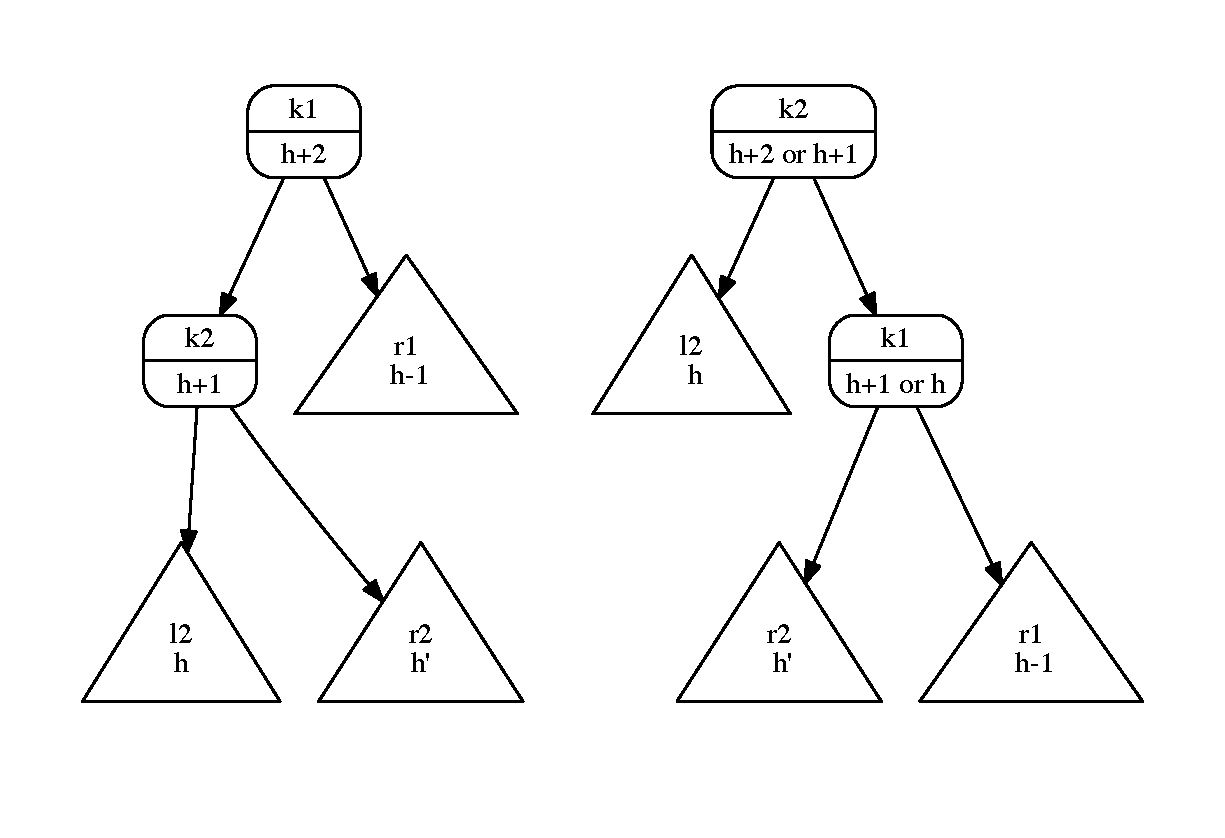
\epsfig{file=casell,scale=0.7}} 
        \caption{Ein unbalancierter Baum und der rebalancierte Baum}
        \label{fig:casell}
      \end{figure}

      Wir m\"ussen uns davon \"uberzeugen, dass der im rechten Teil von Abbildung
      \ref{fig:casell} gezeigte Baum auch tats\"achlich ein AVL-Baum ist.   Was die
      Balancierungs-Bedingung angeht, so rechnet man dies sofort nach.  Die Tatsache,
      dass der mit $k_1$ markierte Knoten entweder die H\"ohe $h$ oder $h+1$ hat folgt
      daraus, dass $r_1$ die H\"ohe $h-1$ hat und dass $h' \in \{h, h-1\}$ gilt.

      Um zu sehen, dass
      der Baum geordnet ist, k\"onnen wir  folgende Ungleichung hinschreiben: \\[0.2cm]
      \hspace*{1.3cm} $l_2 < k_2 < r_2 < k_1 < r_1$. \hspace*{\fill} $(\star)$\\[0.2cm]
      Dabei  schreiben wir f\"ur einen Schl\"ussel $k$ und einen Baum $b$ \\[0.2cm]
      \hspace*{1.3cm} $k < b$ \\[0.2cm]
      um auzudr\"ucken, dass $k$ kleiner ist als alle Schl\"ussel, die in dem Baum $b$ vorkommen.
      Analog schreiben wir $b < k$ wenn alle Schl\"ussel, die in dem Baum $b$ vorkommen,
      kleiner sind als der Schl\"ussel $k$.  Die Ungleichung $(\star)$ beschreibt die Anordnung
      der Schl\"ussel sowohl f\"ur den im linken Teil der Abbildung gezeigten Baum als auch
      f\"ur den Baum im rechten Teil der Abbildung und damit sind beide B\"aume geordnet.
\item $\begin{array}[t]{cl}
               & l_1.\textsl{height}() = r_1.\textsl{height}() + 2    \\ 
        \wedge & l_1 = \textsl{node}(k_2,v_2,l_2,r_2)               \\
        \wedge & l_2.\textsl{height}() < r_2.\textsl{height}()     \\
        \wedge & r_2 = \textsl{node}(k_3,v_3,l_3,r_3)               \\
        \rightarrow & \textsl{node}(k_1,v_1,l_1,r_1).\textsl{restore}() = 
                      \textsl{node}\bigl(k_3,v_3,\textsl{node}(k_2,v_2,l_2,l_3),\textsl{node}(k_1,v_1,r_3,r_1) \bigr)
        \end{array}
       $

        Die linke Seite der  Gleichung wird durch die Abbildung \ref{fig:caselr} auf Seite
        \pageref{fig:caselr}
        illustriert.  Dieser Baum kann in der Form \\[0.2cm]
        \hspace*{1.3cm} 
        $\textsl{node}\bigl(k_1,v_1,\textsl{node}(k_2,v_2,l_2,\textsl{node}\bigl(k_3,v_3,l_3,r_3)\bigr),r_1\bigr)$ \\[0.2cm]
        geschrieben werden. Die Teilb\"aume $l_3$ und $r_3$ haben hier entweder die H\"ohe $h$ oder
        $h-1$, wobei mindestens einer der beiden Teilb\"aume die H\"ohe $h$ haben muss.
\begin{figure}[!ht]
  \centering
  \framebox{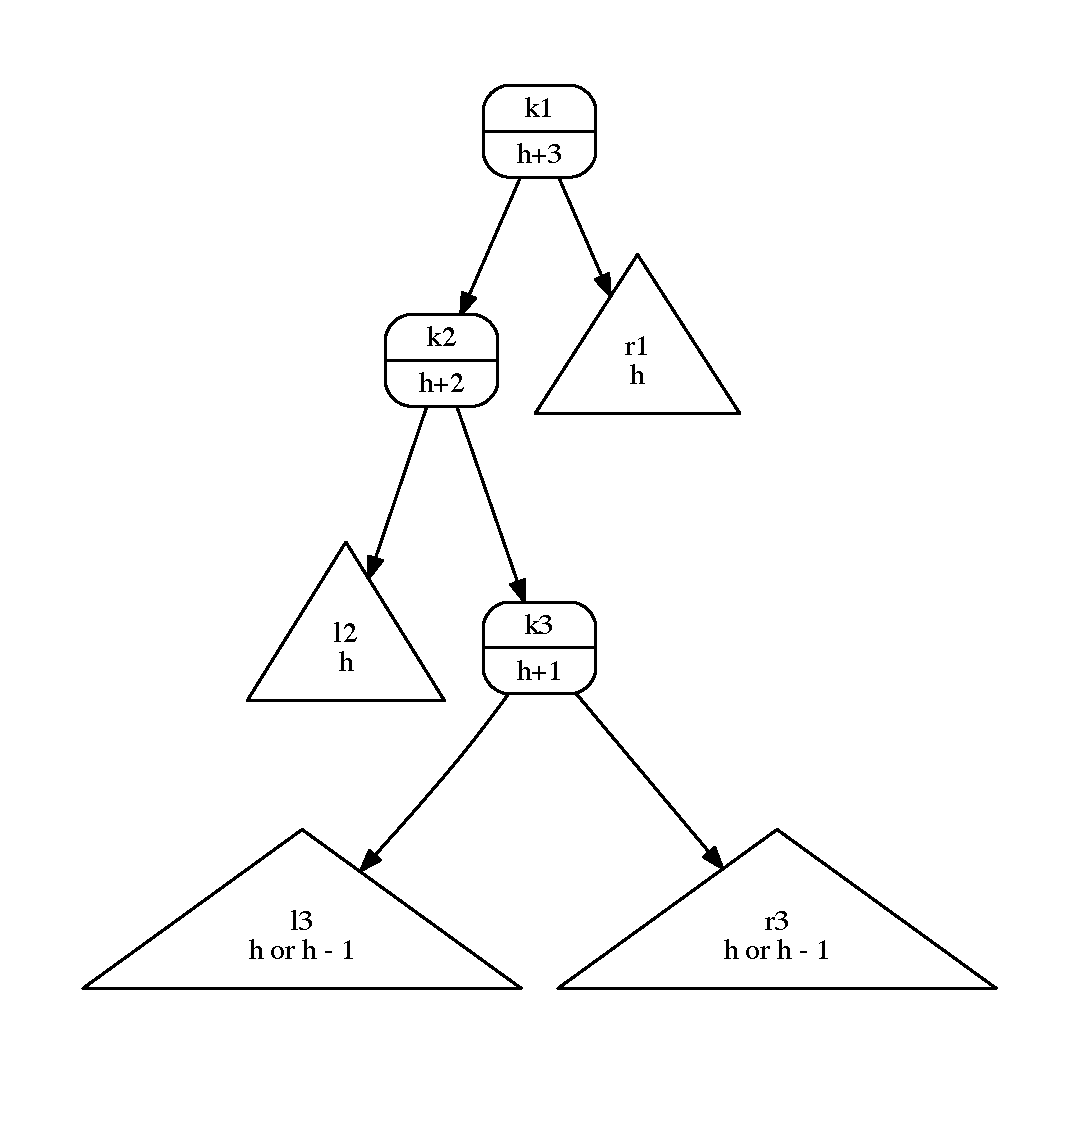
\epsfig{file=caselr,scale=0.7}} 
  \caption{Ein unbalancierter Baum: 2. Fall}
  \label{fig:caselr}
\end{figure}

     Die Situation der rechten Seite der obigen Gleichung zeigt Abbildung
     \ref{fig:caselr-nach} auf Seite \pageref{fig:caselr-nach}.  Der auf dieser
     Abbildung gezeigte Baum hat die Form \\[0.2cm]
     \hspace*{1.3cm} 
     $\textsl{node}\bigl(k_3,v_3,\textsl{node}(k_2,v_2,l_2,l_3),\textsl{node}(k_1,v_1,r_3,r_1) \bigr)$.


\begin{figure}[!ht]
  \centering
  \framebox{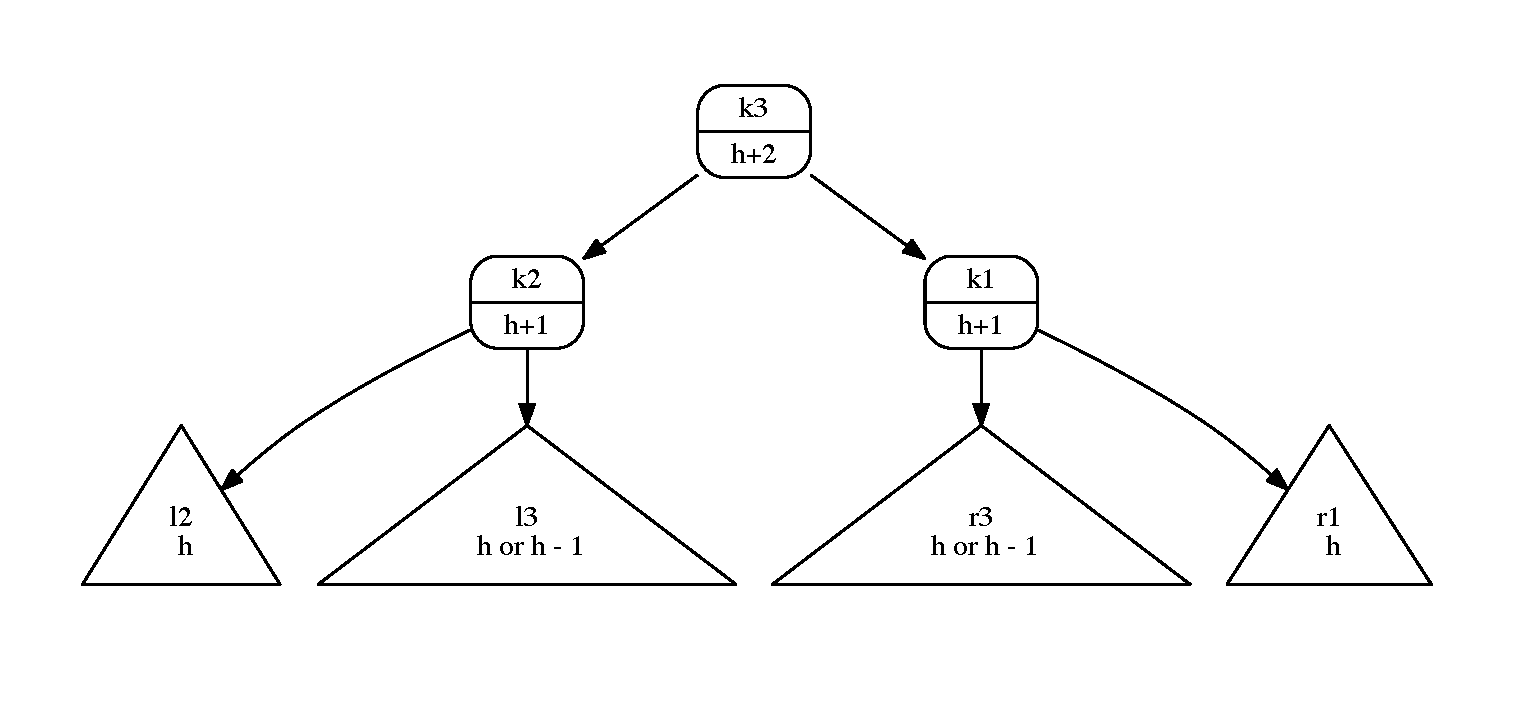
\epsfig{file=caselr-nach,scale=0.7}} 
  \caption{Der rebalancierte Baum im 2. Fall}
  \label{fig:caselr-nach}1
\end{figure}

      Die Ungleichung, die die Anordnung der Schl\"ussel sowohl im linken als auch rechten
      Baum wieder gibt, lautet\\[0.2cm]
      \hspace*{1.3cm} $l_2 < k_2 < l_3 < k_3 < r_3 < k_1 < r_1$.

      Es gibt noch zwei weitere F\"alle die auftreten, wenn der rechte Teilbaum um mehr als
      Eins gr\"o{\ss}er ist als der linke Teilbaum.  Diese beiden F\"alle sind aber zu den beiden
      vorherigen F\"allen v\"ollig analog, so dass wir die Gleichungen hier ohne weitere
      Diskussion angeben.
\item $\begin{array}[t]{cl}
              & r_1.\textsl{height}() = l_1.\textsl{height}() + 2    \\ 
       \wedge & r_1 = \textsl{node}(k_2,v_2,l_2,r_2)               \\
       \wedge & r_2.\textsl{height}() \geq l_2.\textsl{height}()     \\[0.2cm]
       \rightarrow & \textsl{node}(k_1,v_1,l_1,r_1).\textsl{restore}() = 
                     \textsl{node}\bigl(k_2,v_2,\textsl{node}(k_1,v_1,l_1,l_2),r_2\bigr)
       \end{array}
      $
\item $\begin{array}[t]{cl}
               & r_1.\textsl{height}() = l_1.\textsl{height}() + 2    \\ 
        \wedge & r_1 = \textsl{node}(k_2,v_2,l_2,r_2)               \\
        \wedge & r_2.\textsl{height}() < l_2.\textsl{height}()     \\
        \wedge & l_2 = \textsl{node}(k_3,v_3,l_3,r_3)               \\
        \rightarrow & \textsl{node}(k_1,v_1,l_1,r_1).\textsl{restore}() = 
                      \textsl{node}\bigl(k_3,v_3,\textsl{node}(k_1,v_1,l_1,l_3),\textsl{node}(k_2,v_2,r_3,r_2) \bigr)
        \end{array}
       $

\end{enumerate}
Damit k\"onnen wir nun die Methode $\textsl{insert}()$ durch bedingte rekursive Gleichungen 
beschreiben.  Dabei m\"ussen wir die urspr\"unglich f\"ur geordnete B\"aume angegebene Gleichungen
dann \"andern, wenn die Balancierungs-Bedingung durch das Einf\"ugen eines neuen Elements
verletzt werden kann.
\begin{enumerate}
\item $\textsl{nil}\mathtt{.}\textsl{insert}(k,v) = \textsl{node}(k,v, \textsl{nil}, \textsl{nil})$.  
\item $\textsl{node}(k, v_2, l, r)\mathtt{.}\textsl{insert}(k,v_1) = \textsl{node}(k, v_1, l, r)$.
\item $k_1 < k_2 \rightarrow 
          \textsl{node}(k_2, v_2, l, r)\mathtt{.}\textsl{insert}(k_1, v_1) =
          \textsl{node}\bigl(k_2, v_2, l\mathtt{.}\textsl{insert}(k_1, v_1), r\bigr).\textsl{restore}()$.
\item $k_1 > k_2 \rightarrow 
         \textsl{node}(k_2, v_2, l, r)\mathtt{.}\textsl{insert}(k_1, v_1) = 
         \textsl{node}\bigl(k_2, v_2, l, r\mathtt{.}\textsl{insert}(k_1, v_1)\bigr).\textsl{restore}()$.
\end{enumerate}
Analog \"andern sich die Gleichungen f\"ur $\textsl{delMin}()$ wie folgt:
\begin{enumerate}
\item $\textsl{node}(k, v, \textsl{nil}, r)\mathtt{.}\textsl{delMin}() = \langle r, k, v \rangle$.
\item $l\not= \textsl{nil} \wedge l\mathtt{.}\textsl{delMin}() = \langle l',k_{min}, v_{min}\rangle 
       \;\rightarrow$ \\[0.2cm]
       \hspace*{1.3cm} 
       $\textsl{node}(k, v, l, r)\mathtt{.}\textsl{delMin}() = 
        \langle \textsl{node}(k, v, l', r).\textsl{restore}(), k_{min}, v_{min} \rangle$.
\end{enumerate}
Damit k\"onnen wir die Gleichungen zur Spezifikation der  Methode $\mathtt{delete}()$ angeben.
\begin{enumerate}
\item $\textsl{nil}\mathtt{.}\textsl{delete}(k) = \textsl{nil}$.
\item $\textsl{node}(k,v,\textsl{nil},r)\mathtt{.}\textsl{delete}(k) = r$.
\item $\textsl{node}(k,v,l,\textsl{nil})\mathtt{.}\textsl{delete}(k) = l$.
\item $l \not= \textsl{nil} \,\wedge\, r \not= \textsl{nil} \,\wedge\, 
       r\mathtt{.}\textsl{delMin}() = \langle r',k_{min}, v_{min} \rangle  \;\rightarrow$ \\[0.2cm]
      \hspace*{1.3cm}
      $\textsl{node}(k,v,l,r)\mathtt{.}\textsl{delete}(k) = \textsl{node}(k_{min},v_{min},l,r').\textsl{restore}()$.
\item $k_1 < k_2 \rightarrow \textsl{node}(k_2,v_2,l,r)\mathtt{.}\textsl{delete}(k_1) = 
       \textsl{node}\bigl(k_2,v_2,l\mathtt{.}\textsl{delete}(k_1),r\bigr).\textsl{restore}()$.
\item $k_1 > k_2 \rightarrow \textsl{node}(k_2,v_2,l,r)\mathtt{.}\textsl{delete}(k_1) = 
       \textsl{node}\bigl(k_2,v_2,l,r\mathtt{.}\textsl{delete}(k_1)\bigr).\textsl{restore}()$.
\end{enumerate}

\subsection{Implementierung von AVL-B\"aumen in \textsl{Java}}
 
\begin{figure}[!ht]
  \centering
\begin{Verbatim}[ frame         = lines, 
                  framesep      = 0.3cm, 
                  labelposition = bottomline,
                  numbers       = left,
                  numbersep     = -0.2cm,
                  xleftmargin   = 0.8cm,
                  xrightmargin  = 0.8cm
                ]
    public class AVLTree<Key extends Comparable<Key>, Value> 
        implements MyMap<Key, Value>
    {
        Node<Key, Value> mRoot; 
        
        public AVLTree() {
            mRoot = new EmptyNode<Key, Value>();
        }
        public Value find(Key key) {
            return mRoot.find(key);
        }
        public void insert(Key key, Value value) {
            mRoot = mRoot.insert(key, value);
        }
        public void delete(Key key) {
            mRoot = mRoot.delete(key);
        }
    }
    \end{Verbatim}
\vspace*{-0.3cm}
  \caption{Die Klasse \textsl{AVLTree}.}
  \label{fig:AVLTree.java}
\end{figure}

\noindent
Abbildung \ref{fig:AVLTree.java} auf Seite \pageref{fig:AVLTree.java} zeigt die Implementierung
der Klasse \textsl{AVLTree}.  Gegen\"uber der Implementierung der Klasse \textsl{BinaryTree}
aus Abbildung \ref{fig:BinTree.java} auf Seite \pageref{fig:BinTree.java} wurde hier nur der Name
der Klasse ge\"andert.

\begin{figure}[!ht]
  \centering
\begin{Verbatim}[ frame         = lines, 
                  framesep      = 0.3cm, 
                  labelposition = bottomline,
                  numbers       = left,
                  numbersep     = -0.2cm,
                  xleftmargin   = 0.8cm,
                  xrightmargin  = 0.8cm
                ]
    public abstract class Node<Key extends Comparable<Key>, Value>
    {
        protected int mHeight;  // the height of the tree
    
        public abstract Value find(Key key);
        public abstract Node<Key, Value> insert(Key key, Value value);
        public abstract Node<Key, Value> delete(Key key);
        public abstract boolean          isEmpty();
        
        abstract Triple<Node<Key, Value>, Key, Value> delMin();
        abstract void                                 restore();
    }
\end{Verbatim}
\vspace*{-0.3cm}
  \caption{Die abstrakte Klasse \textsl{Node}.}
  \label{fig:Node-AVL.java}
\end{figure}

Abbildung \ref{fig:Node-AVL.java} auf Seite \pageref{fig:Node-AVL.java} zeigt die neue
Implementierung der abstrakten Klasse \textsl{Node}.  Gegen\"uber der Implementierung in Abbildung
\ref{fig:Node.java} auf Seite \pageref{fig:Node.java} ist hier einerseits in Zeile 3 die
Member-Variable \texttt{mHeight} neu hinzu gekommen und andererseits gibt es jetzt in
Zeile 11 die Methode $\textsl{restore}()$, mit deren Hilfe sich die
Balancierungs-Bedingung wiederherstellen l\"asst, wenn diese durch eine Einf\"uge- oder
L\"osch-Operation verletzt worden ist.


\begin{figure}[!ht]
  \centering
\begin{Verbatim}[ frame         = lines, 
                  framesep      = 0.3cm, 
                  labelposition = bottomline,
                  numbers       = left,
                  numbersep     = -0.2cm,
                  xleftmargin   = 0.8cm,
                  xrightmargin  = 0.8cm
                ]
    public class EmptyNode<Key extends Comparable<Key>, Value> 
        extends Node<Key, Value>
    {
        public EmptyNode() {
            mHeight = 0;
        }       
        public Value find(Key key) { 
            return null; 
        }
        public Node<Key, Value> insert(Key key, Value value) {
            return new BinaryNode<Key, Value>(key, value);
        }       
        public Node<Key, Value> delete(Key key) {
            return this;
        }    
        public boolean isEmpty() {
            return true;
        }
        Triple<Node<Key, Value>, Key, Value> delMin() {
            throw new UnsupportedOperationException();
        }
        void restore() {}
    }
\end{Verbatim}
\vspace*{-0.3cm}
  \caption{Die Klasse \textsl{EmptyNode}.}
  \label{fig:EmptyNode-AVL.java}
\end{figure}

Abbildung \ref{fig:EmptyNode-AVL.java} auf Seite \pageref{fig:EmptyNode-AVL.java}
zeigt die Implementierung der Klasse \textsl{EmptyNode}.  Gegen\"uber der in
Abbildung \ref{fig:EmptyNode.java} auf Seite \pageref{fig:EmptyNode.java} gezeigten
Implementierung gibt es zwei kleine \"Anderungen:
\begin{enumerate}
\item In Zeile 5 setzt der Konstruktor die H\"ohe \texttt{mHeight} auf 0.
\item In Zeile 22 ist die Methode $\textsl{restore}()$ implementiert.  Diese
      Implementierung ist f\"ur einen leeren Knoten trivial.
\end{enumerate}

\begin{figure}[!ht]
  \centering
\begin{Verbatim}[ frame         = lines, 
                  framesep      = 0.3cm, 
                  labelposition = bottomline,
                  numbers       = left,
                  numbersep     = -0.2cm,
                  xleftmargin   = 0.2cm,
                  xrightmargin  = 0.2cm
                ]
    public class BinaryNode<Key extends Comparable<Key>, Value> 
        extends Node<Key, Value>
    {
        private Key              mKey;
        private Value            mValue;
        private Node<Key, Value> mLeft;
        private Node<Key, Value> mRight;
    
        public BinaryNode(Key key, Value value) {
            mKey    = key;
            mValue  = value;
            mLeft   = new EmptyNode<Key, Value>();
            mRight  = new EmptyNode<Key, Value>();
            mHeight = 1;
        }    
        public BinaryNode(Key key, Value value, Node<Key, Value> left, 
                                                Node<Key, Value> right) {
            mKey    = key;
            mValue  = value;
            mLeft   = left;
            mRight  = right;
            mHeight = 1 + Math.max(mLeft.mHeight, mRight.mHeight);
        }
        public Value find(Key key) {
            int cmp = key.compareTo(mKey);
            if (cmp < 0) {                // key < mKey
                return mLeft.find(key);
            } else if (cmp > 0) {         // key > mKey
                return mRight.find(key);
            } else {                      // key == mKey
                return mValue;
            }           
        }
        public Node<Key, Value> insert(Key key, Value value) {
            int cmp = key.compareTo(mKey);
            if (cmp < 0) {                        // key < mKey
                mLeft = mLeft.insert(key, value);
            } else if (cmp > 0) {                 // key > mKey
                mRight = mRight.insert(key, value);
            } else {                              // key == mKey
                mValue = value;
            }
            restore();
            return this;
        }
\end{Verbatim}
\vspace*{-0.3cm}
  \caption{Die Klasse \textsl{BinaryNode}, Teil \texttt{I}.}
  \label{fig:BinaryNode-AVL-I.java}
\end{figure}

\begin{figure}[!ht]
  \centering
\begin{Verbatim}[ frame         = lines, 
                  framesep      = 0.3cm, 
                  firstnumber   = last,
                  labelposition = bottomline,
                  numbers       = left,
                  numbersep     = -0.2cm,
                  xleftmargin   = 0.2cm,
                  xrightmargin  = 0.2cm
                ]
        public Node<Key, Value> delete(Key key) {
            int cmp = key.compareTo(mKey);
            if (cmp == 0) {
                if (mLeft.isEmpty()) {
                    return mRight;
                } 
                if (mRight.isEmpty()) {
                    return mLeft;
                }
                Triple<Node<Key, Value>, Key, Value> triple = mRight.delMin();
                mRight = triple.getFirst();
                mKey   = triple.getSecond();
                mValue = triple.getThird();
            }
            if (cmp < 0) {
                mLeft = mLeft.delete(key);
            }
            if (cmp > 0) {
                mRight = mRight.delete(key);
            }
            restore();
            return this;
        }
        public boolean isEmpty() {
            return false;
        }    
        Triple<Node<Key, Value>, Key, Value> delMin() {
            if (mLeft.isEmpty()) {
                return new Triple(mRight, mKey, mValue);
            } else {
                Triple<Node<Key, Value>, Key, Value> t = mLeft.delMin();
                mLeft = t.getFirst();
                Key   key   = t.getSecond();
                Value value = t.getThird();
                restore();
                return new Triple(this, key, value);
            }
        }
\end{Verbatim}
\vspace*{-0.3cm}
  \caption{Die Klasse \textsl{BinaryNode}, Teil \texttt{II}.}
  \label{fig:BinaryNode-AVL-II.java}
\end{figure}

\begin{figure}[!ht]
  \centering
\begin{Verbatim}[ frame         = lines, 
                  framesep      = 0.3cm, 
                  firstnumber   = last,
                  labelposition = bottomline,
                  numbers       = left,
                  numbersep     = -0.2cm,
                  commandchars  = \\\{\},
                  xleftmargin   = 0.2cm,
                  xrightmargin  = 0.2cm
                ]
        void restore() \{
            if (Math.abs(mLeft.mHeight - mRight.mHeight) <= 1) \{
                restoreHeight();
                return;
            \}
            if (mLeft.mHeight > mRight.mHeight) \{
                Key   k1 = mKey;
                Value v1 = mValue;
                BinaryNode<Key, Value> l1 = (BinaryNode<Key, Value>) mLeft;
                Node<Key, Value>  r1 = mRight;
                Key   k2 = l1.mKey;
                Value v2 = l1.mValue;
                Node<Key, Value> l2 = l1.mLeft;
                Node<Key, Value> r2 = l1.mRight;
                if (l2.mHeight >= r2.mHeight) \{
                    mKey   = k2;
                    mValue = v2;
                    mLeft  = l2;
                    mRight = new BinaryNode<Key, Value>(k1, v1, r2, r1);
                \} else \{
                    BinaryNode<Key, Value> rb2 = (BinaryNode<Key, Value>) r2;
                    Key   k3 = rb2.mKey;
                    Value v3 = rb2.mValue;
                    Node<Key, Value>  l3 = rb2.mLeft;
                    Node<Key, Value>  r3 = rb2.mRight;
                    mKey   = k3;
                    mValue = v3;
                    mLeft  = new BinaryNode<Key, Value>(k2, v2, l2, l3);
                    mRight = new BinaryNode<Key, Value>(k1, v1, r3, r1);
                \}
            \}
            if (mRight.mHeight > mLeft.mHeight) \{
               \(\vdots\)
            \}
            restoreHeight();
        \}
        void restoreHeight() \{
            mHeight = 1 + Math.max(mLeft.mHeight, mRight.mHeight);
        \}
    \}
\end{Verbatim}
\vspace*{-0.3cm}
  \caption{Die Klasse \textsl{BinaryNode}, Teil \texttt{III}.}
  \label{fig:BinaryNode-AVL-III.java}
\end{figure}

Die Abbildungen \ref{fig:BinaryNode-AVL-I.java}, \ref{fig:BinaryNode-AVL-II.java} und
\ref{fig:BinaryNode-AVL-III.java} auf Seite \pageref{fig:BinaryNode-AVL-I.java}
und den folgenden Seiten zeigen die Implementierung der Klasse \textsl{BinaryNode}.
Gegen\"uber der entsprechenden Implementierung in den Abbildungen
\ref{fig:BinaryNode-I.java} und \ref{fig:BinaryNode-II.java} 
auf den Seiten \pageref{fig:BinaryNode-I.java} und \pageref{fig:BinaryNode-II.java} 
gibt es die folgenden \"Anderungen:
\begin{enumerate}
\item In dem ersten Konstruktor wird in Zeile 14 die Member-Variable \texttt{mHeight} auf
      1 gesetzt.
\item In Zeile 16 -- 23 haben wir einen neuen Konstruktor,
      der neben einem Schl\"ussel und einem Wert als zus\"atzliche Argumente noch den
      linken und den rechten Teilbaum des neu zu erstellenden Knoten erh\"alt.
      Dieser Konstruktor wird sp\"ater f\"ur die Implementierung der Methode $\textsl{restore}()$
      ben\"otigt.
\item Die Implementierung von $\textsl{find}()$ hat sich gegen\"uber der alten Implementierung 
      nicht ver\"andert, den jeder AVL-Baum ist ja auch ein geordneter bin\"arer Baum.
\item Am Ende der Methode \textsl{insert}() wird in Zeile 43 die Methode
      $\textsl{restore}()$ aufgerufen um die Balancierungs-Bedingung sicherzustellen. 

      Eigentlich m\"usste die Methode $\textsl{restore}()$ nur dann aufgerufen werden,
      wenn entweder im linken oder im rechten Teilbaum ein neuer Schl\"ussel eingef\"ugt wird.  Es w\"urde also
      reichen, die Methode am Ende der  \texttt{if}-Bl\"ocken in Zeile 37 und 39 aufzurufen.
      Dann h\"atten wir aber zwei Aufrufe von $\textsl{restore}()$.  Der Code wird 
      \"ubersichtlicher, wenn $\textsl{restore}()$ am Ende der Methode aufgerufen wird.
\item Genauso wird in Zeile 66 vor der Beendigung der Methode $\textsl{delete}()$
      die Methode $\textsl{restore}()$ aufgerufen.

      Entscheidend ist hier zu bemerken, dass sich die Implementierung der beiden Methoden
      $\textsl{insert}()$ und $\textsl{delete}()$  gegen\"uber der Implementierung,
      die wir f\"ur geordnete bin\"are B\"aume verwendet haben, nur an einer einzigen Stelle
      ge\"andert hat:  Wir m\"ussen nur vor dem \texttt{return}-Befehl
      $\textsl{restore}()$ aufrufen.
\item Auch die Implementierung von $\textsl{delMin}()$ unterscheidet sich von der alten
      Implementierung nur durch den Aufruf von $\textsl{restore}()$ in Zeile 80.
\item In Zeile 84 implementieren wir die Methode $\textsl{restore}()$.
      \begin{enumerate}
      \item Falls die Balancierungs-Bedingung bereits erf\"ullt ist, so muss die Methode
            $\textsl{restore}()$ nur daf\"ur sorgen, dass die Member-Variable \texttt{mHeight} an dem Knoten
            korrekt gesetzt ist.  Dazu wird die Methode Methode $\textsl{restoreHeight()}$
            aufgerufen.  Diese Methode ist in Zeile 120 -- 122 implementiert und berechnet
            die H\"ohe neu.
      \item Falls die H\"ohe des linken Teilbaums nun gr\"o{\ss}er als die H\"ohe des rechten
            Teilbaums ist und au{\ss}erdem die Balancierungs-Bedingung verletzt ist,
            dann gibt es eine weitere Fall-Unterscheidung, die wir bei der Herleitung
            der bedingten Gleichungen zur Spezifikation der Methode $\textsl{restore}()$
            bereits diskutiert hatten.  Diese beiden F\"alle werden in Zeile 89 -- 113
            behandelt.

            In den Zeilen 98 -- 102 behandeln wir den Fall, der in Abbildung
            \ref{fig:casell} gezeigt ist, w\"ahrend die Zeilen 104 -- 112 
            den Fall behandeln, der in den Abbildungen \ref{fig:caselr} und
            \ref{fig:caselr-nach} dargestellt wird.
      \item Der Code, der den Fall betrachtet, in dem einerseits
            die H\"ohe des rechten Teilbaums  gr\"o{\ss}er als die H\"ohe des linken
            Teilbaums ist und andererseits die Balancierungs-Bedingung verletzt ist,
            ist v\"ollig analog zu dem vorigen Fall und wird deshalb in der Abbildung nicht
            explizit wiedergegeben.
      \item In Zeile 118 wird am Ende der Methode $\textsl{restore}()$ noch daf\"ur gesorgt,
            dass die Member-Variable \texttt{mHeight} an dem Knoten aktualsisiert wird.
      \end{enumerate}
\end{enumerate}


\subsection{Analyse der Komplexit\"at}
Wir analysieren jetzt die Komplexit\"at von AVL-B\"aumen im schlechtesten Fall. Der
schlechteste Fall tritt dann ein, wenn bei einer vorgegebenen Zahl von Schl\"usseln die H\"ohe
maximal wird.  Das ist aber dasselbe wie wenn in einem Baum gegebener H\"ohe die Zahl der
Schl\"ussel minimal wird.  Wir definieren daher $b_h(k)$ als einen AVL-Baum der H\"ohe $h$, der
unter allen AVL-B\"aumen der H\"ohe $h$ die minimale Anzahl von Schl\"usseln hat.  Au{\ss}erdem
sollen alle Schl\"ussel, die in $b_h(k)$ auftreten, gr\"o{\ss}er als der Schl\"ussel $k$ sein.
Sowohl die Schl\"ussel als auch die Werte sind in diesem Zusammenhang eigentlich unwichtig,
wir m\"ussen nur darauf achten, dass die Ordnungs-Bedingung f\"ur bin\"are B\"aume erf\"ullt ist.
Wir werden f\"ur die Schl\"ussel nat\"urliche Zahlen nehmen, f\"ur die Werte nehmen wir immer die
Zahl $0$.  Bevor wir mit der Definition von $b_h(k)$ beginnen k\"onnen, ben\"otigen wir noch eine
Hilfs-Funktion $\textsl{maxKey}()$ mit der Signatur  
\[ \textsl{maxKey}:\mathcal{B}_< \rightarrow \textsl{Key} \]
F\"ur einen gegebenen geordneten nicht-leeren bin\"aren Baum $b$ 
berechnet $b.\textsl{maxKey}()$ den gr\"o{\ss}ten Schl\"ussel, der in $b$ auftritt.  Die
Definition von $b.\textsl{maxKey}()$ ist induktiv:
\begin{enumerate}
\item $\textsl{node}(k,v,l,\textsl{nil}).\textsl{maxKey}() = k$,
\item $r \not= \textsl{nil} \rightarrow \textsl{node}(k,v,l,r).\textsl{maxKey}() = r.\textsl{maxKey}()$.
\end{enumerate}
Damit k\"onnen wir nun die B\"aume $b_h(k)$ durch Induktion nach der H\"ohe $h$ definieren.
\begin{enumerate}
\item $b_0(k) = nil$,

      denn es gibt genau einen AVL-Baum der H\"ohe $0$ und dieser enth\"alt keinen Schl\"ussel.
\item $b_1(k) = \textsl{node}(k+1,0,\textsl{nil}, \textsl{nil})$,

      denn es gibt genau einen AVL-Baum der H\"ohe $1$.
\item $b_{h+1}(k).\textsl{maxKey}() = l \rightarrow 
       b_{h+2}(k) = \textsl{node}\bigl(l+1,\,0,\,b_{h+1}(k),\,b_h(l+1)\bigr)$,

      denn um einen AVL-Baum der H\"ohe $h+2$ mit einer minimalen Anzahl an Schl\"usseln zu
      konstruieren, erzeugen wir zun\"achst den AVL-Baum $b_{h+1}(k)$ der H\"ohe $h+1$.
      Dann bestimmen wir den maximalen Schl\"ussel $l$ in diesem Baum, der Schl\"ussel $l+1$
      kommt nun an die Wurzel des zu erzeugenden Baums der H\"ohe $h+2$ und schlie{\ss}lich erzeugen wir noch
      den Baum $b_h(l+1)$ der H\"ohe $h$, den wir als rechten Teilbaum in den neu zu
      erzeugenden Baum der H\"ohe $h+2$  einf\"ugen.
\end{enumerate}
F\"ur einen beliebigen bin\"aren Baum $b$ bezeichne $\#\,b$ die Anzahl der Schl\"ussel, die in
$b$ auftreten.  Dann definieren wir 
\\[0.2cm]
\hspace*{1.3cm}
$c_h := \#\, b_h(k)$
\\[0.2cm]
als die Anzahl der Schl\"ussel des Baums $b_h(k)$.  Wir werden sofort sehen, dass
$\#\,b_h(k)$ nicht von $k$ abh\"angt.  F\"ur $c_h$ finden wir in Analogie zu
der induktiven Definition von $b_h(k)$ die folgenden Gleichungen.
\begin{enumerate}
\item $c_0 = \#\, b_0(k) = \#\, \textsl{nil} = 0$,
\item $c_1 = \#\, b_1(k) = \#\, \textsl{node}(k+1,0,\textsl{nil}, \textsl{nil}) = 1$, 
\item$\begin{array}[t]{lcl}
       c_{h+2} & = & \#\, b_{h+2}(k) \\
               & = & \#\,\textsl{node}\bigl(l+1,\,0,\,b_{h+1}(k),\,b_h(l+1)\bigr) \\
               & = & \#\, b_{h+1}(k) + \#\, b_h(l+1) + 1 \\
               & = & c_{h+1} + c_h + 1.
       \end{array}$
\end{enumerate}
Also haben wir zur Bestimmung von $c_h$ die Rekurrenz-Gleichung
\\[0.2cm]
\hspace*{1.3cm}
$c_{h+2} = c_{h+1} + c_h + 1 \quad \mbox{mit den Anfangs-Bedingungen $c_0 = 0$ und $c_1 = 1$}$
\\[0.2cm]
zu l\"osen.  Das ist eine Rekurrenz-Gleichung,
die wir, allerdings mit leicht ver\"anderten Anfangs-Bedingungen, bereits im dritten Kapitel gel\"ost haben.
Sie k\"onnen leicht nachrechnen, dass die L\"osung dieser Rekurrenz-Gleichung wie folgt
lautet: 
\\[0.2cm]
\hspace*{1.3cm}
$c_h = \displaystyle \frac{1}{\sqrt{5}} \left( \lambda_1^{h+2} - \lambda_2^{h+2} \right) -
1$  \quad mit
\\[0.2cm]
\hspace*{1.3cm}
$\lambda_1 = \displaystyle \frac{1}{2}(1 + \sqrt{5}) \approx  1.62$ \quad und \quad $\lambda_2 =
\displaystyle \frac{1}{2}(1 - \sqrt{5}) \approx -0.62$.
\\[0.2cm]
Da $|\lambda_2| < 1$ ist, spielt der Wert $\displaystyle\lambda_2^{h+2}$
f\"ur gro{\ss}e Werte von $h$   praktisch keine Rolle und die
minimale Zahl $n$ der Schl\"ussel in einem Baum der H\"ohe $h$ ist durch \\[0.2cm]
\hspace*{1.3cm} $n \approx \displaystyle \frac{1}{\sqrt{5}} \lambda_1^{h+2} - 1$ \\[0.2cm]
gegeben.  Um diese Gleichung nach $h$ aufzul\"osen, bilden wir auf beiden Seiten den
Logarithmus zur Basis 2.  Dann erhalten wir 
\\[0.2cm]
\hspace*{1.3cm}
$\log_2(n+1) = (h+2) \cdot \log_2(\lambda_1) - \frac{1}{2}\cdot \log_2(5)$
\\[0.2cm]
Daraus folgt nach Addition von $\frac{1}{2}\cdot \log_2(5)$
\\[0.2cm]
\hspace*{1.3cm}
$\log_2(n+1) + \frac{1}{2}\cdot \log_2(5) = (h+2) \cdot \log_2(\lambda_1)$
\\[0.2cm]
Jetzt teilen wir durch $\log_2(\lambda_1)$.  Dann erhalten wir 
\\[0.4cm]
\hspace*{1.3cm}
$\displaystyle \bruch{\log_2(n+1) + \frac{1}{2}\cdot \log_2(5)}{\log_2(\lambda_1)} = h+2$
\\[0.2cm]
L\"osen wir diese Gleichung nach $h$ auf, so haben wir f\"ur gro{\ss}e $n$
das Ergebnis
\\[0.4cm]
\hspace*{0.3cm} 
$h = \displaystyle \bruch{\log_2(n+1) + \frac{1}{2}\cdot \log_2(5)}{\log_2(\lambda_1)} - 2 =
      \bruch{1}{\log_2(\lambda_1)}\cdot \log_2(n) + \Oh(1) \approx 1,44 \cdot \log_2(n) + \Oh(1)$ 
\\[0.2cm]
gewonnen. 
Die Gr\"o{\ss}e $h$ gibt aber die Zahl der Vergleiche an, die wir im ung\"unstigsten Fall bei
einem Aufruf von \textsl{find} in einem AVL-Baum mit $n$ Schl\"usseln durchf\"uhren m\"ussen.
Wir sehen also, dass bei einem AVL-Baum auch im schlechtesten Fall die Komplexit\"at
logarithmisch bleibt.  Abbildung
\ref{fig:avl-worst-case} zeigt einen AVL-Baum der H\"ohe 6, f\"ur den das Verh\"altnis von H\"ohe zur Anzahl
der Knoten maximal wird.  Wie man sieht ist auch dieser Baum noch sehr weit weg von dem
zur Liste entarteten Baum aus der Abbildung \ref{fig:degenerated}.


\begin{figure}[!ht]
  \centering
  \framebox{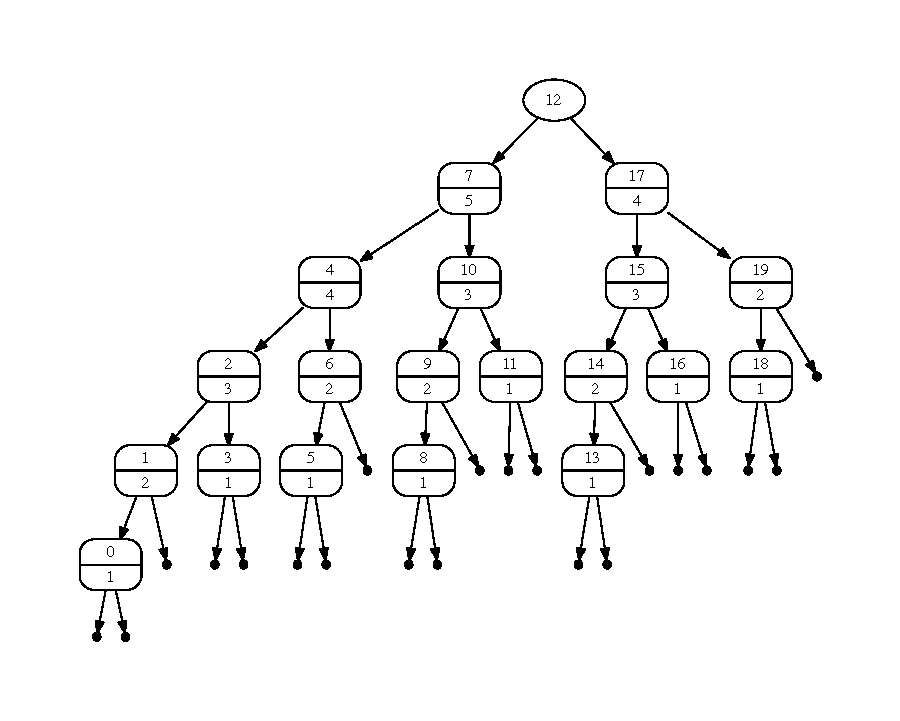
\epsfig{file=avl}} 
  \caption{Ein AVL-Baum mit dem ung\"unstigsten Verh\"altnis von H\"ohe zur Anzahl an Knoten}
  \label{fig:avl-worst-case}
\end{figure}
\pagebreak
\vspace*{\fill}

\pagebreak


\section{Tries}
In der Praxis kommt es h\"aufig vor, dass die Schl\"ussel des ADT \textsl{Map} Strings sind.
In dem einf\"uhrenden Beispiel des elektronischen Telefon-Buchs ist dies der Fall.  Es gibt eine
Form von Such-B\"aumen, die auf diese Situation besonders angepasst ist.  Diese Such-B\"aume
haben den Namen \emph{Tries}.  Dieses Wort ist von dem Englischen Wort
\emph{re\underline{trie}val} abgeleitet. Damit man \emph{Tries} und \emph{Trees}
unterscheiden kann, wird \emph{Trie} so ausgesprochen, dass es sich mit dem Englischen
Wort \emph{pie} reimt.  Diese Datenstruktur wurde 1959 von Ren\'e de la Briandais
\cite{briandais:59} vorgeschlagen.


Die Grundidee bei der Datenstruktur \emph{Trie} ist ein Baum, an dem jeder Knoten nicht
nur zwei Nachfolger hat, wie das bei bin\"aren B\"aumen der Fall ist, sondern stattdessen
potentiell f\"ur jeden Buchstaben des Alphabets einen Ast besitzt.  Um Tries definieren zu
k\"onnen, nehmen wir zun\"achst an, dass folgendes gegeben ist:
\begin{enumerate}
\item $\Sigma$ ist eine endliche Menge, deren Elemente wir als \emph{Buchstaben}
      bezeichnen. $\Sigma$ selbst hei{\ss}t das \emph{Alphabet}.
\item $\Sigma^*$ bezeichnet die Menge der \emph{W\"orter} (engl.~\emph{strings}), die wir aus den Buchstaben
      des Alphabets bilden k\"onnen.  Mathematisch k\"onnen wir W\"orter als Listen von 
      Buchstaben auffassen. Ist $w \in \Sigma^*$ so schreiben wir $w = cr$, falls
      $c$ der erste Buchstabe von $w$ ist und $r$ das Wort ist, das durch L\"oschen des
      ersten Buchstabens aus $w$ entsteht.  

      In \textsl{Java} k\"onnen wir sp\"ater $c$ und $r$ wie
      folgt aus dem String $w$ gewinnen: \\[0.2cm]
      \hspace*{1.3cm} $c = w.\textsl{charAt}(0)\mathtt{;}$ 
      \quad und \quad $r = w.\textsl{substring}(1)\mathtt{;}$
\item $\varepsilon$ bezeichnet das leere Wort.  In \textsl{Java} k\"onnen wir schreiben \\[0.2cm]
      \hspace*{1.3cm} $\mathtt{epsilon} = \symbol{34}\symbol{34}\mathtt{;}$ 
\item \textsl{Value} ist eine Menge von \emph{Werten}.  
\end{enumerate}
Die Menge $\mathbb{T}$ der Tries definieren wir nun induktiv mit Hilfe des 
Konstruktors \\[0.2cm]
\hspace*{1.3cm} 
$\textsl{node}: \textsl{Value} \times \textsl{List}(\Sigma) \times
\textsl{List}(\mathbb{T}) \rightarrow \mathbb{T}$. \\[0.2cm]
Die induktive Definition besteht nur aus einer einzigen Klausel. Falls
\begin{enumerate}
\item $v \in \textsl{Value} \cup \{\Omega\}$
\item $C = [c_1, \cdots, c_n] \in \textsl{List}(\Sigma)$ eine Liste von Buchstaben der
      L\"ange $n$ ist,
\item $T = [t_1, \cdots, t_n] \in \textsl{List}(\mathbb{T})$ eine Liste von Tries derselben L\"ange $n$ ist, 
\end{enumerate}
dann gilt \\[0.2cm]
\hspace*{1.3cm}  $\textsl{node}(v, C, T) \in \mathbb{T}$.  \\[0.2cm]
Als erstes fragen Sie sich
vermutlich, wo bei dieser induktiven Definition der Induktions-Anfang ist.
Der Induktions-Anfang ist der Fall $n=0$, denn dann sind die Listen $L$ und $T$ leer.

Als n\"achstes \"uberlegen wir uns, welche Funktion von dem Trie \\[0.2cm]
\hspace*{1.3cm}  $\textsl{node}(v, [c_1, \cdots, c_n], [t_1, \cdots, t_n]) \in \mathbb{T}$ \\[0.2cm]
dargestellt wird.  Wir beantworten diese Frage, indem wir rekursive Gleichungen f\"ur die
Methode \\[0.2cm]
\hspace*{1.3cm} $\textsl{find}: \mathbb{T} \times \Sigma^* \rightarrow \textsl{Value} \cup \{ \Omega\}$
\\[0.2cm]
angeben.  Wir werden den Ausdruck $\textsl{node}(v,L,T).\textsl{find}(s)$ durch Induktion \"uber den String $s$
definieren:
\begin{enumerate}
\item $\textsl{node}(v, C, T).\textsl{find}(\varepsilon) = v$.

      Der dem leeren String zugeordnete Wert wird also unmittelbar an der Wurzel
      des Tries abgespeichert.
\item $\textsl{node}(v, [c_1, \cdots, c_n], [t_1, \cdots, t_n]).\textsl{find}(cr) = 
        \left\{
        \begin{array}{ll}
        t_1.\textsl{find}(r) & \mbox{falls} \quad c = c_1 \mbox{;} \\
        \vdots &                                     \\
        t_i.\textsl{find}(r) & \mbox{falls} \quad c = c_i \mbox{;} \\
        \vdots &                                     \\
        t_n.\textsl{find}(r) & \mbox{falls} \quad c = c_n \mbox{;} \\[0.2cm]
        \Omega               & \mbox{falls} \quad c \notin \{c_1,\cdots,c_n\} \mbox{.}         
        \end{array}
       \right.$

      Der Trie $\textsl{node}(v, [c_1, \cdots, c_n], [t_1, \cdots, t_n])$ enth\"alt also genau
      dann einen Wert zu dem Schl\"ussel $cr$, wenn einerseits der Buchstabe $c$ in der Buchstaben-Liste
      an der Stelle $i$ auftritt und wenn andererseits der Trie $t_i$ einen Wert zu dem
      Schl\"ussel $r$ enth\"alt.
\end{enumerate}

\begin{figure}[!ht]
  \centering
  \framebox{\epsfig{file=trie}} 
  \caption{Ein Beispiel Trie}
  \label{fig:trie}
\end{figure}

Zum besseren Verst\"andnis wollen wir Tries graphisch als B\"aume darstellen.
Nun ist es nicht sinnvoll, die Knoten dieser B\"aume mit langen Listen zu beschriften.
Wir behelfen uns mit einem Trick.  Um einen Knoten der Form \\[0.2cm]
\hspace*{1.3cm} 
$\textsl{node}(v, [c_1, \cdots, c_n], [t_1, \cdots, t_n])$ \\[0.2cm]
darzustellen, zeichnen wir einen Kreis,
den wir durch einen horizontalen Strich in der Mitte aufteilen.
Falls $v$ von $\Omega$ verschieden ist, schreiben wir den Wert $v$ in die untere H\"alfte
des Kreises.
(Bei den in Abbildung \ref{fig:trie} gezeigten Kreisen handelt es sich um
Mutantenkreise.)
Das, was wir \"uber dem Strich schreiben,
h\"angt von dem Vater des jeweiligen Knotens ab.  Wie genau es vom Vater abh\"angt, sehen wir gleich.
Der Knoten selber hat $n$ Kinder. Diese $n$ Kinder sind die 
Wurzeln der B\"aume, die die Tries $t_1$, $\cdots$, $t_n$ darstellen.
Au{\ss}erdem markieren wir die diese Knoten darstellenden Kreise in den oberen H\"alfte 
mit den Buchstaben $c_1$, $\cdots$, $c_n$.  


Zur Verdeutlichung geben wir ein Beispiel in 
Abbildung \ref{fig:trie} auf Seite \pageref{fig:trie}.
Die Funktion, die hier dargestellt wird, l\"asst sich wie folgt als bin\"are Relation
schreiben: \\[0.2cm]
\hspace*{1.3cm} $ \bigl\{ \langle \textrm{``Stahl''},   1  \rangle, \langle \textrm{``Stolz''},     2  \rangle, \langle \textrm{``Stoeger''},   3  \rangle, 
             \langle \textrm{``Salz''},      4  \rangle, \langle \textrm{``Schulz''},    5  \rangle$, \\[0.2cm]
\hspace*{1.5cm} $\langle \textrm{``Schulze''},   6  \rangle, \langle \textrm{``Schnaut''},   7  \rangle, 
  \langle \textrm{``Schnupp''},   8  \rangle, 
  \langle \textrm{``Schroer''},   9  \rangle\}$. \\[0.2cm]
Der Wurzel-Knoten ist hier leer, denn dieser Knoten hat keinen Vater-Knoten, von dem er
eine Markierung erben k\"onnte.  Diesem Knoten entspricht der Term \\[0.2cm]
\hspace*{1.3cm} $\textsl{node}(\Omega,[\textrm{`S'}], [t])$. \\[0.2cm]
Dabei bezeichnet $t$ den Trie, dessen Wurzel mit dem Buchstaben `S' markiert ist.
Diesen Trie k\"onnen wir seinerseits durch den Term \\[0.2cm]
\hspace*{1.3cm} 
$\textsl{node}(\Omega,[\textrm{`t'},\textrm{`a'},\textrm{`c'}], [t_1, t_2, t_3])$ \\[0.2cm]
darstellen.  Daher hat dieser Knoten drei S\"ohne, die mit den Buchstaben `t', `a' und `c'
markiert sind.

\subsection{Einf\"ugen in Tries}
Wir stellen nun bedingte Gleichungen auf, mit denen wir das Einf\"ugen eines Schl\"ussels mit
einem zugeh\"origen Wert beschreiben k\"onnen.  Bezeichnen wir die Methode f\"ur das Einf\"ugen
mit $\textsl{insert}()$, so hat diese Methode die Signatur
\\[0.2cm]
\hspace*{1.3cm}
$\textsl{insert}: \mathbb{T} \times \Sigma^* \times V \rightarrow \mathbb{T}$.
\\[0.2cm]
Wir definieren den Wert von \\[0.2cm]
\hspace*{1.3cm} $\textsl{node}(v, [c_1, \cdots, c_n], [t_1, \cdots, t_n]).\textsl{insert}(s,v)$\\[0.2cm]
f\"ur ein Wort $w\in \Sigma^*$ und einen Wert $v \in V$
durch Induktion nach der L\"ange des Wortes $w$.
\begin{enumerate}
\item $\textsl{node}(v_1,L,T).\textsl{insert}(\varepsilon, v_2) = \textsl{node}(v_2,L,T)$,

      Einf\"ugen eines Wertes mit dem leeren String als Schl\"ussel \"uberschreibt also einfach
      den an dem Wurzel-Knoten gespeicherten Wert. 
\item $\textsl{node}\bigl(v_1,[c_1,\cdots,c_i,\cdots,c_n], [t_1,\cdots,t_i,\cdots,t_n]\bigr).\textsl{insert}(c_ir,v_2) =$ \\[0.2cm]
      \hspace*{1.3cm}  
      $\textsl{node}\bigl(v_1,[c_1,\cdots,c_i,\cdots,c_n], [t_1,\cdots,t_i.\textsl{insert}(r,v_2),\cdots,t_n]\bigr)$.

      Wenn in dem Trie $\textsl{node}\bigl(v_1,[c_1,\cdots,c_i,\cdots,c_n], [t_1,\cdots,t_i,\cdots,t_n]\bigr)$ ein Wert
      $v_2$ zu dem Schl\"ussel $cr$ eingef\"ugt werden soll, und falls der Buchstabe $c$ in der Liste $[c_1,\cdots,c_n]$
      an der Stelle $i$ vorkommt, wenn also gilt $c= c_i$, dann muss der Wert $v_2$
      rekursiv in dem Trie $t_i$ unter dem Schl\"ussel 
      $r$ eingef\"ugt werden.

\item $c \not\in\{c_1,\cdots,c_n\} \;\rightarrow\;\textsl{node}\bigl(v_1,[c_1,\cdots,c_n], [t_1,\cdots,t_n]\bigr).\textsl{insert}(cr,v_2) =$ \\[0.2cm]
      \hspace*{1.3cm}  
      $\textsl{node}\bigl(v_1,[c_1,\cdots,c_n,c], [t_1,\cdots,t_n,\textsl{node}(\Omega,[],[]).\textsl{insert}(r,v_2)]\bigr)$.
      
      Wenn in dem Trie $\textsl{node}\bigl(v_1,[c_1,\cdots,c_n], [t_1,\cdots,t_n]\bigr)$
      ein Wert $v_2$ zu dem Schl\"ussel $cr$ eingef\"ugt werden soll, und falls der Buchstabe
      $c$ in der Liste $[c_1,\cdots,c_n]$ nicht vorkommt, dann wird zun\"achst ein Trie
      erzeugt, der die leere Abbildung repr\"asentiert.  Dieser Trie hat die Form \\[0.2cm]
      \hspace*{1.3cm} $\textsl{node}(\Omega, [], [])$. \\[0.2cm]
      Anschlie{\ss}end wird in diesem Trie der Wert $v_2$ rekursiv unter dem Schl\"ussel $r$
      eingef\"ugt. Zum Schluss h\"angen wir den Buchstaben $c$ an die Liste $[c_1,\cdots,c_n]$
      an und f\"ugen den Trie  \\[0.2cm] 
      \hspace*{1.3cm} $\textsl{node}(\Omega, [], []).\textsl{insert}(r,v_2)$ \\[0.2cm]
      am Ende der Liste $[t_1,\cdots,t_n]$ ein.
\end{enumerate}

\subsection{L\"oschen in Tries}
Als letztes stellen wir die bedingten Gleichungen auf, die das L\"oschen von
Schl\"usseln und den damit verkn\"upften Werten in einem Trie beschreiben.
Um diese Gleichungen einfacher schreiben zu k\"onnen, definieren wir zun\"achst eine
Hilfs-Funktion \\[0.2cm]
\hspace*{1.3cm} $\textsl{isEmpty}: \mathbb{T} \rightarrow \mathbb{B}$, \\[0.2cm]
so dass $t.\textsl{isEmpty}()$ genau dann $\mathtt{true}$ liefert, wenn der Trie
$t$ die leere Funktion darstellt.  Wir definieren also: 
\begin{enumerate}
\item $\textsl{node}(\Omega, [],[]).\textsl{isEmpty}() = \mathtt{true}$
\item $v \not= \Omega \rightarrow 
       \textsl{node}(v, [c_1,\cdots,c_n],[t_1,\cdots,t_n]).\textsl{isEmpty}() = \mathtt{false}$
\item $\textsl{node}(\Omega, L, T).\textsl{isEmpty}() = \textsl{isEmptyList}(T)$
\end{enumerate}
In der letzten Gleichung haben wir eine weitere Hilfs-Funktion benutzt, die wir noch
definieren m\"ussen.  Die Funktion
\\[0.2cm]
\hspace*{1.3cm}
$\textsl{isEmptyList}: \textsl{List}(\mathbb{T}) \rightarrow \mathbb{B}$
\\[0.2cm]
pr\"uft f\"ur eine gegebene Liste von Tries, ob alle in der Liste vorhandenen Tries leer sind.
Die Definition dieser Funktion erfolgt durch Induktion \"uber die L\"ange der Liste.
\begin{enumerate}
\item $\textsl{isEmptyList}\bigl([]\bigr) = \mathtt{true}$,
\item $\textsl{isEmptyList}\bigl([t] + R\bigr) = 
       \bigl(t.isEmpty() \wedge \textsl{isEmptyList}(R)\bigr)$,

      denn alle Tries in der Liste $[t]+R$ sind leer, wenn einerseits $t$ ein leerer
      Trie ist und wenn andererseits auch alle Tries in $R$ leer sind.
\end{enumerate}
Nun k\"onnen wir die Methode
\\[0.2cm]
\hspace*{1.3cm}
$\textsl{delete}: \mathbb{T} \times \Sigma^* \rightarrow \mathbb{T}$
\\[0.2cm]
spezifizieren:  Wir definieren den Wert von \\[0.2cm]
\hspace*{1.3cm} 
$t.\textsl{delete}(w)$
\\[0.2cm]
f\"ur einen Trie $t \in \mathbb{B}$ und ein Wort $w \in \Sigma^*$
durch Induktion nach der L\"ange des Wortes $w$.
\begin{enumerate}
\item $\textsl{node}(v,L,T).\textsl{delete}(\varepsilon) = \textsl{node}(\Omega,L,T)$,

      denn der Wert, der unter dem leeren String $\varepsilon$ in einem Trie
      gespeichert wird, befindet sich unmittelbar an der Wurzel des Tries und
      kann dort sofort gel\"oscht werden.
\item $\begin{array}[t]{ll}
       t_i.\textsl{delete}(r).\textsl{isEmpty}()   & \rightarrow \\
       \textsl{node}(v, [c_1,\cdots,c_i,\cdots,c_n],[t_1,\cdots,t_i,\cdots,t_n]).\textsl{delete}(c_ir) 
       & = \\
       \qquad 
       \textsl{node}(v, [c_1,\cdots,c_{i-1},c_{i+1},\cdots,c_n],[t_1,\cdots,t_{i-1},t_{i+1},\cdots,t_n]).
       \end{array}
       $

       Wenn der zu l\"oschende String mit dem Buchstaben $c_i$ anf\"angt, und wenn
       das L\"oschen des Schl\"ussels $r$ in dem $i$-ten Trie $t_i$ einen leeren
       Trie ergibt, dann streichen wir den $i$-ten Buchstaben und den dazu
       korrespondierenden $i$-ten Trie $t_i$.
\item $\begin{array}[t]{ll}
       \neg t_i.\textsl{delete}(r).\textsl{isEmpty}()   & \wedge \\
       \textsl{node}(v, [c_1,\cdots,c_i,\cdots,c_n],[t_1,\cdots,t_i,\cdots,t_n]).\textsl{delete}(c_ir) 
       & = \\
       \qquad \textsl{node}(v, [c_1,\cdots,c_i,\cdots,c_n],[t_1,\cdots,t_i.\textsl{delete}(r),\cdots,t_n]).
       \end{array}
       $

       Wenn der zu l\"oschende String mit dem Buchstaben $c_i$ anf\"angt, und wenn
       der Baum $t_i$, der durch das  L\"oschen des Schl\"ussels $r$ in dem $i$-ten
       Trie $t_i$ entsteht nicht leer ist, dann l\"oschen wir rekursiv in dem Baum $t_i$ den Schl\"ussel
       $r$.
\item $c \notin C \rightarrow \textsl{node}(v, C, T).\textsl{delete}(cr) = \textsl{node}(v, C, T)$.

       Wenn der zu l\"oschende String mit dem Buchstaben $c$ anf\"angt und wenn der
       Buchstabe $c$ gar kein Element der Buchstaben-Liste $C$ des Tries
       ist, dann ver\"andert das L\"oschen den Trie nicht.
\end{enumerate}

\subsection{Implementierung in \textsl{Java}}
Wir zeigen nun, wie sich die Tries in \textsl{Java} implementieren lassen.
Die Abbildungen \ref{fig:TrieNode-I} und \ref{fig:TrieNode-II} auf den Seiten
\pageref{fig:TrieNode-I} und 
\pageref{fig:TrieNode-II} zeigen die Implementierung, die wir jetzt diskutieren.

\begin{figure}[!ht]
  \centering
\begin{Verbatim}[ frame         = lines, 
                  framesep      = 0.3cm, 
                  labelposition = bottomline,
                  numbers       = left,
                  numbersep     = -0.2cm,
                  xleftmargin   = 0.2cm,
                  xrightmargin  = 0.2cm
                ]
    import java.util.*;
    
    public class TrieNode<Value> implements MyMap<String, Value>
    {
        Value                      mValue;
        ArrayList<Character>       mCharList;
        ArrayList<TrieNode<Value>> mNodeList;
    
        TrieNode() {
            mValue    = null;
            mCharList = new ArrayList<Character>(0);
            mNodeList = new ArrayList<TrieNode<Value>>(0);
        }    
        public Value find(String key) {
            if (key.length() == 0) {
                return mValue;
            } else {
                Character firstChar = key.charAt(0);
                String    rest      = key.substring(1);
                for (int i = 0; i < mCharList.size(); ++i) {
                    if (firstChar.equals(mCharList.get(i))) {
                        return mNodeList.get(i).find(rest);
                    }
                }
                return null;
            }
        }
        public void insert(String key, Value value) {
            if (key.length() == 0) {
                mValue = value;
            } else {
                Character firstChar = key.charAt(0);
                String    rest      = key.substring(1);
                for (int i = 0; i < mCharList.size(); ++i) {
                    if (firstChar.equals(mCharList.get(i))) {
                        mNodeList.get(i).insert(rest, value);
                        return;
                    }
                }
                mCharList.add(firstChar);
                TrieNode<Value> node = new TrieNode<Value>();
                node.insert(rest, value);
                mNodeList.add(node);
            }
        }
\end{Verbatim}
\vspace*{-0.3cm}
  \caption{Die Klasse \textsl{TrieNode-I}, Teil \texttt{I}.}
  \label{fig:TrieNode-I}
\end{figure}

\begin{enumerate}
\item Den Trie $\textsl{node}(v, [c_1,\cdots,c_n], [t_1,\cdots,t_n])$ stellen wir durch ein Objekt der Klasse
      \textsl{TrieNode} dar.  Diese Klasse hat drei Member-Variablen:
      \begin{enumerate}
      \item \texttt{mValue} entspricht dem Wert $v$, der an der Wurzel des Tries
             gespeichert ist.
      \item \texttt{mCharList} entspricht der Buchstaben-Liste $[c_1,\cdots,c_n]$.
      \item \texttt{mNodeList} entspricht der Trie-Liste $[t_1,\cdots,t_n]$.
      \end{enumerate}
\item Der Konstruktor in Zeile 9 erzeugt den Trie $\textsl{node}(\Omega, [], [])$, der die
      leere Funktion repr\"asentiert.
\item Die Implementierung der Methode \textsl{find} orientiert sich genau an den Gleichungen, 
      mit denen wir diese Methode spezifiziert haben.
      \begin{enumerate}
      \item Falls der Schl\"ussel, nach dem wir suchen, der leere String ist,
            geben wir den Wert \texttt{mValue} zur\"uck.
      \item Sonst hat der Schl\"ussel die Form $\textsl{key} = cr$. Wir setzen
            $\textsl{firstChar} = c$ und $\textsl{rest} = r$.  Wir gehen nun die
            Buchstaben-Liste \texttt{mCharList} durch und schauen, ob wir 
            dabei den Buchstaben $c$ finden.  Wenn  wir den Buchstaben $c$ an der $i$-ten
            Stelle finden, dann suchen wir anschlie{\ss}end  in dem $i$-ten Trie in der Liste 
            \texttt{mNodeList} nach dem Schl\"ussel $r$.

            Falls der Buchstabe $c$ nicht gefunden wird, geben wir \texttt{null} zur\"uck um
            den speziellen Wert $\Omega$ zu repr\"asentieren.
      \end{enumerate}
\item Die Implementierung der Methode \textsl{insert} ist analog zu der Implementierung
      der Methode \textsl{find}.
      \begin{enumerate}
      \item Falls der Schl\"ussel, unter dem wir den Wert \textsl{value} einf\"ugen wollen, der
            leere String ist, k\"onnen  wir die Member-Variable \texttt{mValue} \"uberschreiben.
      \item Sonst hat der Schl\"ussel die Form $\textsl{key} = cr$. Wir setzen wieder
            $\textsl{firstChar} = c$ und $\textsl{rest} = r$.  Wir gehen nun die
            Buchstaben-Liste \texttt{mCharList} durch und suchen den Buchstaben $c$.  
            Wenn wir $c$ an der $i$-ten
            Stelle finden, dann f\"ugen wir anschlie{\ss}end  in dem $i$-ten Trie in der Liste 
            \texttt{mNodeList} den Wert \texttt{value} unter dem Schl\"ussel $r$ ein.

            Falls der Buchstabe $c$ nicht in der Liste \texttt{mCharList} auftritt,
            dann f\"ugen wir $c$ am Ende der Buchstaben-Liste ein.  Gleichzeitig erzeugen
            wir einen zun\"achst leeren Trie, in dem wir dann den Wert \texttt{value} unter dem
            Schl\"ussel $r$ einf\"ugen.  Diesen Trie f\"ugen wir an das Ende der Liste
            \texttt{mNodeList} ein.            
      \end{enumerate}
\item Als letztes diskutieren wir die Implementierung der Methode \textsl{delete}.
      \begin{enumerate}
      \item Falls der Schl\"ussel, den wir l\"oschen wollen, der
            leere String ist, so setzen wir einfach die Member-Variable \texttt{mValue}
            auf \texttt{null}.
      \item Sonst hat der Schl\"ussel die Form $\textsl{key} = cr$. Wir setzen wieder
            $\textsl{firstChar} = c$ und $\textsl{rest} = r$.  Wir gehen nun die
            Buchstaben-Liste \texttt{mCharList} durch und suchen den Buchstaben $c$
            finden.  Wenn wir $c$ an der $i$-ten 
            Stelle finden, dann l\"oschen wir in dem $i$-ten Trie in der Liste 
            \texttt{mNodeList} den Schl\"ussel $r$.  Falls dieser Trie jetzt leer ist,
            so l\"oschen wir einerseits diesen Trie aus \texttt{mNodeList} und andererseits
            l\"oschen wir den Buchstaben $c_i$ aus der Liste \texttt{mCharList}.

            Falls der Buchstabe $c$ nicht in der Liste \texttt{mCharList} auftritt,
            so ist nichts weiter zu tun, denn in diesem Fall sind in dem Trie keinerlei
            Informationen zu dem Schl\"ussel \textsl{key} gespeichert.
      \end{enumerate}
\end{enumerate}

\begin{figure}[!ht]
  \centering
\begin{Verbatim}[ frame         = lines, 
                  framesep      = 0.3cm, 
                  firstnumber   = last,
                  labelposition = bottomline,
                  numbers       = left,
                  numbersep     = -0.2cm,
                  xleftmargin   = 0.2cm,
                  xrightmargin  = 0.2cm
                ]
        public void delete(String key) {
            if (key.length() == 0) {
                mValue = null;
                return;
            } 
            Character firstChar = key.charAt(0);
            String    rest      = key.substring(1);
            for (int i = 0; i < mCharList.size(); ++i) {
                if (firstChar.equals(mCharList.get(i))) {
                    TrieNode<Value> node = mNodeList.get(i);
                    node.delete(rest);
                    if (node.isEmpty()) {
                        mCharList.remove(i);
                        mNodeList.remove(i);
                    } 
                    return;
                }
            }
        }
        public Boolean isEmpty() {
            return mValue == null && mNodeList.size() == 0;
        }
    }
\end{Verbatim}
\vspace*{-0.3cm}
  \caption{Die Klasse \textsl{TrieNode}, Teil \texttt{II}.}
  \label{fig:TrieNode-II}
\end{figure}

\noindent
\textbf{Bemerkung}:  Falls das Alphabet $\Sigma$ viele Buchstaben enth\"alt, 
k\"onnen die Listen $[c_1, \cdots, c_n]$ und $[t_1,\cdots,t_n]$, die in einem Trie  der Form
\\[0.2cm]
\hspace*{1.3cm}
$\textsl{node}(v, [c_1, \cdots, c_n], [t_1,\cdots,t_n])$
\\[0.2cm]
abgespeichert sind, lang werden.  Dann ist es eventuell effizienter, die Buchstaben-Liste
$[c_1, \cdots, c_n]$ zu sortieren.  Dann k\"onnte die Methode $\textsl{find}()$
effizienter implementiert werden.  Allerdings wird das Einf\"ugen und L\"oschen in diesem Fall komplizierter.
\vspace*{0.3cm}


\noindent
\textbf{Bin\"are Tries}:  Wir nehmen im Folgenden an, dass unser Alphabet nur aus den beiden
Ziffern $0$ und $1$ besteht, es gilt also $\Sigma = \{0,1\}$.  Dann k\"onnen wir nat\"urliche
Zahlen als Worte aus $\Sigma^*$ auffassen.  Wir wollen die Menge der \emph{bin\"aren Tries}
mit $\BT$ bezeichnen und wie folgt induktiv definieren:
\begin{enumerate}
\item $\textsl{nil} \in \BT$.
\item $\textsl{bin}(v,l,r) \in \BT$ falls
      \begin{enumerate}
      \item $v \in \textsl{Value} \cup \{\Omega\}$.
      \item $l,r \in \BT$.
      \end{enumerate}
\end{enumerate}
Die Semantik legen wir fest, indem wir eine Methode 
\\[0.2cm]
\hspace*{1.3cm}
$\textsl{find}: \BT \times \mathbb{N} \rightarrow \textsl{Value} \cup \{ \Omega \}$
\\[0.2cm]
definieren.  F\"ur einen bin\"aren Trie $b$ und eine nat\"urliche Zahl $n$ gibt
$b.\textsl{find}(n)$ den Wert zur\"uck, der unter dem Schl\"ussel $n$ in dem bin\"aren Trie $b$ gespeichert ist.
Falls in dem bin\"aren Trie $b$ unter dem Schl\"ussel $n$ kein Wert gespeichert ist, wird
$\Omega$ zur\"uck gegeben.
Formal definieren wir den Wert von $b.\textsl{find}(n)$ durch Induktion nach dem Aufbau
von $b$.  Im Induktions-Schritt ist eine Neben-Induktion nach $n$ erforderlich.
\begin{enumerate}
\item $\textsl{nil}.\textsl{find}(n) = \Omega$,

      denn in dem leeren bin\"aren Trie finden wir keine Werte.
\item $\textsl{bin}(v,l,r).\textsl{find}(0) = v$,

      denn der Schl\"ussel $0$ entspricht dem leeren String $\varepsilon$.
\item $n \not= 0 \rightarrow \textsl{bin}(v,l,r).\textsl{find}(2\!\cdot \!n) = l.\textsl{find}(n)$,

      denn wenn wir Zahlen im Bin\"arsystem darstellen, so hat bei geraden Zahlen das letzte
      Bit den Wert 0 und die 0 soll dem linken Teilbaum entsprechen.
\item $\textsl{bin}(v,l,r).\textsl{find}(2\!\cdot \!n\!+\!1) = r.\textsl{find}(n)$,

      denn wenn wir Zahlen im Bin\"arsystem darstellen, so hat bei ungeraden Zahlen das letzte
      Bit den Wert 1 und die 1 soll dem rechten Teilbaum entsprechen.
\end{enumerate}
\textbf{Aufgabe}: 
\begin{enumerate}
\item Stellen Sie Gleichungen auf, die das Einf\"ugen und das L\"oschen in einem
      bin\"aren Trie beschreiben.  Achten Sie beim L\"oschen darauf,
      dass bin\"are Tries der Form $\textsl{bin}(\Omega, \textsl{nil}, \textsl{nil})$
      zu $\textsl{nil}$ vereinfacht werden.

      \textbf{Hinweis}:  Um die Gleichungen zur Spezifikation der Funktion
      $\textsl{delete}()$ nicht zu komplex werden zu lassen ist es sinnvoll, eine
      Hilfsfunktion zur Vereinfachung von bin\"aren Tries zu definieren.
\item Implementieren Sie bin\"are Tries in \textsl{Java}.
\end{enumerate}
\textbf{Bemerkung}: Bin\"are Tries werden auch als \emph{digitale Suchb\"aume} bezeichnet.
\pagebreak


\section{Hash-Tabellen}
Eine Abbildung \\[0.2cm]
\hspace*{1.3cm} $f: \textsl{Key} \rightarrow \textsl{Value}$ \\[0.2cm]
kann dann sehr einfach implementiert werden, wenn \\[0.2cm]
\hspace*{1.3cm} $\textsl{Key} = \{ 0, 1, 2, \cdots, n \}$, \\[0.2cm]
denn dann reicht es aus, ein Feld der Gr\"o{\ss}e $n+1$ zu verwenden.
Abbildung \ref{fig:ArrayMap} zeigt, dass sich der ADT \textsl{Map} 
in diesem Fall trivial implementieren l\"asst.

\begin{figure}[!ht]
  \centering
\begin{Verbatim}[ frame         = lines, 
                  framesep      = 0.3cm, 
                  labelposition = bottomline,
                  numbers       = left,
                  numbersep     = -0.2cm,
                  xleftmargin   = 0.8cm,
                  xrightmargin  = 0.8cm
                ]
    public class ArrayMap<Value> implements MyMap<Integer, Value>
    {
        Value[] mArray;
        
        public ArrayMap(int n) {
            mArray = (Value[]) new Object[n+1];
        }
        public Value find(Integer key) {
            return mArray[key];
        }
        public void insert(Integer key, Value value) {
            mArray[key] = value;
        }
        public void delete(Integer key) {
            mArray[key] = null;
        }
    }
\end{Verbatim}
\vspace*{-0.3cm}
  \caption{Die Klasse \textsl{ArrayMap}.}
  \label{fig:ArrayMap}
\end{figure}


Falls nun der Definitions-Bereich $D$ der darzustellenden Abbildung nicht die Form einer
Menge der Gestalt $\{1, \cdots, n\}$ hat, 
k\"onnten wir versuchen, $D$ zun\"achst auf eine Menge der Form $\{1,\cdots,n\}$ abzubilden.
Wir erl\"autern diese Idee  an einem einfachen Beispiel.
Wir betrachten eine naive Methode um ein Telefon-Buch abzuspeichern:
\begin{enumerate}
\item Wir machen zun\"achst die Annahme, dass alle Namen aus genau  
      8 Buchstaben bestehen.  Dazu werden
      k\"urzere Namen mit Blanks aufgef\"ullt und Namen die l\"anger als 8 Buchstaben sind,
      werden nach dem  8-ten Buchstaben abgeschnitten.
\item Als n\"achstes \"ubersetzen wir Namen in einen Index.  
      Dazu fassen wir die einzelnen Buchstaben als Ziffern auf, die die Werte von 0 bis 26
      annehmen k\"onnen.  Dem Blank ordnen wir dabei den Wert 0 zu.   Nehmen wir an, dass
      die Funktion $\textsl{ord}$ jedem Buchstaben aus der Menge 
      $\Sigma = \{ \texttt{' '}, \texttt{'a'}, \texttt{'b'}, \texttt{'c'}, \cdots, \texttt{'x'}, \texttt{'y'}, \texttt{'z'} \}$ 
      einen Wert aus der Menge
      $\{0,\cdots,26\}$ zuordnet \\[0.2cm]
      \hspace*{1.3cm} 
      $\textsl{ord}: \{ \texttt{' '}, \texttt{'a'}, \texttt{'b'}, \texttt{'c'}, \cdots, \texttt{'x'}, \texttt{'y'}, \texttt{'z'} \} \rightarrow \{0,\cdots, 26\}$,
      \\[0.2cm]
      so l\"asst sich der Wert eines Strings $w = c_0c_1\cdots c_7$ durch eine Funktion \\[0.2cm]
      \hspace*{1.3cm} 
      $\textsl{code}: \Sigma^* \rightarrow \mathbb{N}$ \\[0.2cm]
      berechnen, die wie folgt definiert ist: \\[0.2cm]
      \hspace*{1.3cm} 
      $\textsl{code}(c_0c_1\cdots c_7) = \sum\limits_{i=0}^7 \textsl{ord}(c_i) \cdot 27^i$.
      \\[0.2cm]
      Die Menge \textsl{code} bildet die Menge aller W\"orter mit 8 Buchstaben bijektiv
      auf die Menge der Zahlen $\{0,\cdots,(27^8 - 1)/26\}$ ab.
\end{enumerate}
Leider hat diese naive Implementierung mehrere Probleme: 
\begin{enumerate}
\item Das Feld, das wir anlegen m\"ussen, hat eine Gr\"o{\ss}e von \\[0.2cm]
      \hspace*{1.3cm} $27^8 = 282\,429\,536\,481$ \\[0.2cm]
      Eintr\"agen.  Selbst wenn jeder Eintrag nur die Gr\"o{\ss}e zweier Maschinen-Worte hat und
      ein Maschinen-Wort aus 4 Byte besteht, so br\"auchten wir 
      etwas mehr als ein Terabyte um eine
      solche Tabelle anzulegen.
\item Falls zwei Namen sich erst nach dem 8-ten Buchstaben unterscheiden, k\"onnen 
      wir zwischen diesen Namen nicht mehr unterscheiden. 
\end{enumerate}
Wir k\"onnen diese Probleme wir folgt l\"osen:
\begin{enumerate}
\item Wir \"andern die Funktion \texttt{code} so ab, dass das Ergebnis
      immer kleiner-gleich einer vorgegebene Zahl \texttt{size} ist.  Die Zahl
      \texttt{size} gibt dabei die Gr\"o{\ss}e eines Feldes an und ist so klein,
      dass wir ein solches Feld bequem anlegen k\"onnen.

      Eine einfache M\"oglichkeit, die Funktion \textsl{code} entsprechend abzu\"andern,
      besteht in folgender Implementierung: \\[0.2cm]
      \hspace*{1.3cm} 
      $\textsl{code}(c_0c_1\cdots c_n) = \left(\sum\limits_{i=0}^n \textsl{ord}(c_i) \cdot 27^i\right) \;\%\; \textsl{size}$.
      \\[0.2cm]
      Um eine \"Uberlauf zu vermeiden, k\"onnen wir f\"ur $k=n,n-1,\cdots,1,0$ die Teilsummen $s_k$
      wie folgt induktiv definieren:
      \begin{enumerate}
      \item $s_n = \textsl{ord}(c_n)$
      \item $s_{k} = \left(\textsl{ord}(c_{k}) + s_{k+1} \cdot 27 \right) \;\%\; \textsl{size}$
      \end{enumerate}
      Dann gilt
      \hspace*{1.3cm} 
      $s_0 = \left(\sum\limits_{i=0}^n \textsl{ord}(c_i) \cdot 27^i\right) \;\%\; \textsl{size}$.
      
\item In dem Feld der Gr\"o{\ss}e \textsl{size} speichern wir nun nicht mehr die Werte, sondern stattdessen
      Listen von Paaren aus Schl\"usseln und Werten.  Dies ist notwendig, denn wir k\"onnen
      nicht verhindern, dass die Funktion \texttt{code}() f\"ur zwei verschiedene
      Schl\"ussel den selben Index liefert.
\end{enumerate}
Abbildung \ref{fig:hash-example} auf Seite \pageref{fig:hash-example} zeigt, wie ein Feld,
in dem Listen von Paaren abgebildet sind, aussehen kann.  Ein solches Feld bezeichnen wir
als Hash-Tabelle.  Wir diskutieren nun die Implementierung dieser Idee in \textsl{Java}.


\begin{figure}[!ht]
  \centering
  \framebox{\epsfig{file=hash-table,scale=0.7}} 
  \caption{Eine Hash-Tabelle}
  \label{fig:hash-example}
\end{figure}


\begin{figure}[!ht]
  \centering
\begin{Verbatim}[ frame         = lines, 
                  framesep      = 0.3cm, 
                  labelposition = bottomline,
                  numbers       = left,
                  numbersep     = -0.2cm,
                  xleftmargin   = 0.0cm,
                  xrightmargin  = 0.0cm
                ]
    public class MyHashMap<Key, Value> implements MyMap<Key, Value>
    {
        static final double sAlpha = 2;
        static final int[] sPrimes = { 3, 7, 13, 31, 61, 127, 251, 
             509, 1021, 2039, 4093, 8191, 16381, 32749, 65521, 131071, 
             262139, 524287, 1048573, 2097143, 4194301, 8388593, 16777213, 
             33554393, 67108859, 134217689, 268435399, 536870909, 1073741789, 
             2147483647 
        };
        Object[] mArray;
        int      mPrimeIndex;
        int      mNumberEntries;
    
        public MyHashMap(int primeIndex) {
            mPrimeIndex = primeIndex;
            int size    = sPrimes[mPrimeIndex];
            mArray      = new Object[size];
        }
        public Value find(Key key) {
            int index = Math.abs(key.hashCode() % mArray.length);
            LinkedList<Pair<Key, Value>> list  = 
                (LinkedList<Pair<Key, Value>>) mArray[index];
            if (list == null) {
                return null;
            }
            for (int i = 0; i < list.size(); ++i) {
                Pair<Key, Value> pair = list.get(i);
                if (key.equals(pair.getFirst())) {
                    return pair.getSecond();
                }
            }
            return null;
        }
\end{Verbatim}
\vspace*{-0.3cm}
  \caption{Die Klasse \textsl{MyHashMap}, Teil \texttt{I}.}
  \label{fig:MyHashMap-I}
\end{figure}

\begin{figure}[!ht]
  \centering
\begin{Verbatim}[ frame         = lines, 
                  framesep      = 0.3cm, 
                  firstnumber   = last,
                  labelposition = bottomline,
                  numbers       = left,
                  numbersep     = -0.2cm,
                  xleftmargin   = 0.0cm,
                  xrightmargin  = 0.0cm
                ]
        public void insert(Key key, Value value) {
           if (mNumberEntries / (double) mArray.length > sAlpha) {
                rehash();
            }
            int index = Math.abs(key.hashCode() % mArray.length);
            LinkedList<Pair<Key, Value>> list  = 
                (LinkedList<Pair<Key, Value>>) mArray[index];
            if (list == null) {
                list          = new LinkedList<Pair<Key, Value>>();
                mArray[index] = list;
            }
            for (int i = 0; i < list.size(); ++i) {
                Pair<Key, Value> pair = list.get(i);
                if (key.equals(pair.getFirst())) {
                    pair.setSecond(value);
                    return;
                }
            }
            list.add(new Pair<Key, Value>(key, value));
            ++mNumberEntries;
        }
        private void rehash() {
            ++mPrimeIndex;
            MyHashMap<Key, Value> bigMap = new MyHashMap<Key, Value>(mPrimeIndex);
            for (Object list: mArray) {
                if (list == null) {
                    continue;
                }
                for (Object object: (LinkedList<Pair<Key, Value>>) list) {
                    Pair<Key, Value> pair = (Pair<Key, Value>) object;
                    bigMap.insert(pair.getFirst(), pair.getSecond());
                }
            }
            mArray = bigMap.mArray;
        }
\end{Verbatim}
\vspace*{-0.3cm}
  \caption{Die Klasse \textsl{MyHashMap}, Teil \texttt{II}.}
  \label{fig:MyHashMap-II}
\end{figure}


\begin{figure}[!ht] 
  \centering
\begin{Verbatim}[ frame         = lines, 
                  framesep      = 0.3cm, 
                  firstnumber   = last,
                  labelposition = bottomline,
                  numbers       = left,
                  numbersep     = -0.2cm,
                  xleftmargin   = 0.0cm,
                  xrightmargin  = 0.0cm
                ]
        public void delete(Key key) {
            int index = Math.abs(key.hashCode() % mArray.length);
            LinkedList<Pair<Key, Value>> list  = 
                (LinkedList<Pair<Key, Value>>) mArray[index];
            if (list == null) {
                return;
            }
            for (int i = 0; i < list.size(); ++i) {
                Pair<Key, Value> pair = list.get(i);
                if (key.equals(pair.getFirst())) {
                    list.remove(i);
                    --mNumberEntries;
                    return;
                }
            }
        }
    }
\end{Verbatim}
\vspace*{-0.3cm}
  \caption{Die Klasse \textsl{MyHashMap}, Teil \texttt{III}.}
  \label{fig:MyHashMap-III}
\end{figure}

\begin{enumerate}
\item Als erstes \"uberlegen wir uns, welche Daten-Strukturen wir brauchen,
      um eine Hash-Tabelle zu repr\"asentieren.
      \begin{enumerate}
      \item Wir ben\"otigen ein Feld, indem wir die einzelnen Listen ablegen.
            Dieses Feld wird in Zeile 10 als die Member-Variable \texttt{mArray}
            abgespeichert.

            Es mag Sie verwundern, dass dieses Feld den Typ \texttt{Object[]} hat.
            Eigentlich sollte dieses Feld in der Form \\[0.2cm]
            \hspace*{1.3cm} \texttt{List<Pair<Key, Value>>[] mArray;} \\[0.2cm]
            deklariert werden.  Die Erzeugung generischer Felder ist in \textsl{Java} 
            aber sehr trickreich.  Um nicht zu sehr vom eigentlichen Thema abzukommen
            haben wir daher eine Implementierung gew\"ahlt, die nicht Typ-sicher ist.
      \item Wenn die einzelnen Listen zu gro{\ss} werden, wird die Suche ineffizient.
            Daher ist es notwendig, die Gr\"o{\ss}e dieser Listen zu kontrollieren,
            wenn die Listen zu gro{\ss} werden, muss das Feld vergr\"o{\ss}ert werden.
            Um diesen Prozess zu steuern, m\"ussen wir zun\"achst nachhalten, 
            wieviele Elemente schon in der Hash-Tabelle abgespeichert sind.
            Dies geschieht in der Member-Variable \texttt{mNumberEntries}, die in Zeile 12
            definiert wird.

            Theoretische Untersuchungen, die \"uber den Rahmen der Vorlesung hinausgehen, zeigen, dass
            die Gr\"o{\ss}e der Tabelle eine Primzahl sein sollte.  Daher verf\"ugt der
            Konstruktor \"uber eine Liste von Primzahlen, 
            die in der statistischen Member-Variablen \texttt{sPrimes}, die in Zeile 4
            definiert ist, abgelegt sind.  
            Die $i+1$-te Primzahlen in dieser Liste ist in etwa doppelt so gro{\ss} wie die $i$-te
            Primzahl. Die Member-Variable \texttt{mPrimeIndex}, die
            in Zeile 11 definiert wird, kodiert nun die Gr\"o{\ss}e des
            Feldes \texttt{mArray}.  Es gilt immer \\[0.2cm]
            \hspace*{1.3cm} \texttt{mArray.length == sPrimes[mPrimeIndex]}. \\[0.2cm]
            Die durchschnittliche L\"ange der einzelnen Listen ergibt sich als
            der Quotient aus der Zahl \texttt{mNumberEntries} und der L\"ange des Feldes
            \texttt{mArray}.  Wird nun dieser Wert gr\"o{\ss}er als der
            \emph{Auslastungs-Faktor} (engl.~\emph{load factor})             
            \texttt{sAlpha}, der in Zeile 3 definiert ist, dann verdoppeln wir die Gr\"o{\ss}e
            des Feldes.
      \end{enumerate}
\item Der Konstruktor in Zeile 14 initialsiert \texttt{mPrimeIndex} mit dem gegebenen Argument.
      Wird der Konstruktor zum Beispiel mit dem Argument 0 aufgerufen, dann wird ein Feld
      der L\"ange 3 angelegt, denn es gilt $\texttt{sPrimes[0]} = 3$.
\item Bei der Implementierung der Methode \texttt{find} wandeln wir den gegebenen Schl\"ussel 
      \texttt{key} zun\"achst mit der Methode \texttt{hashCode}() in eine Zahl um.  
      Die Methode \texttt{hashCode}() ist in \textsl{Java} f\"ur jedes Objekt definiert
      und erzeugt eine mehr oder weniger zuf\"allige Zahl, die aber in eindeutiger Weise
      von dem Objekt abh\"angt.  Diese Zahl kann auch negativ sein.
      Wir modifizieren diese Zahl in Zeile 20 durch Bilden von Modulo und Absolutbetrag
      so, dass das Ergebnis in der Menge 
      $\{\,0,\; \cdots,\; \mathtt{mArray.length} - 1\,\}$ liegt.
      Anschlie{\ss}end holen wir die Liste, in der Werte zu dem gegebenen Schl\"ussel
      abgespeichert sein m\"ussen.  Falls in dem Feld an der Stelle, die durch den berechneten 
      Index angegeben wird, noch gar keine Liste gespeichert ist,
      hat die Hash-Tabelle zu dem gegebenen Schl\"ussel noch keinen Eintrag und wir geben in
      Zeile 24 \texttt{null} zur\"uck.

      Andernfalls laufen wir mit einer Schleife durch die Liste durch und vergleichen 
      die einzelnen Schl\"ussel mit dem gegebenen Schl\"ussel \texttt{key}.
      Falls wir den Schl\"ussel finden, geben wir in Zeile 29 den mit diesem Schl\"ussel
      assoziierten Wert zur\"uck.

      Falls wir die Schleife bis zum Ende durchlaufen und den Schl\"ussel nicht gefunden
      haben, dann hat die Hash-Tabelle zu dem gegebenen Schl\"ussel \texttt{key} keinen
      Eintrag und wir geben in Zeile 32 wieder \texttt{null} zur\"uck.

\item Bei der Implementierung der Methode \textsl{insert} berechnen wir zun\"achst den
      aktuellen Auslastungs-Faktor, also die durchschnittliche L\"ange der Listen.  Falls diese L\"ange
      gr\"o{\ss}er als der vorgegebene maximale Auslastungs-Faktor \texttt{sAlpha} ist,
      f\"uhren wir ein sogenanntes \emph{Rehashing} durch, das wir weiter unten im Detail
      diskutieren.

      Anschlie{\ss}end ist die Implementierung analog zur Implementierung der Methode
      \textsl{find}().  Wir berechnen also zun\"achst die Liste, in der Schl\"ussel
      \texttt{key} und der Wert \texttt{value} einzuf\"ugen sind.  Falls unter dem Index
      noch keine Liste existiert, erzeugen wir in den Zeilen 42 und 43 eine neue leere
      Liste und tragen diese Liste in das Feld ein.  

      Anschlie{\ss}end durchlaufen wir die Liste und suchen den Schl\"ussel \texttt{key}.
      Wenn wir den Schl\"ussel finden, dann wird einfach der zugeh\"orige Wert \"uberschrieben.
      Wenn wir den Schl\"ussel \texttt{key} in der Liste nicht finden, dann f\"ugen wir den
      Schl\"ussel zusammen mit dem zugeordneten Wert \texttt{value} in Zeile 52 an das Ende der Liste an.
      Gleichzeitig m\"ussen wir in diesem Fall die Zahl der Eintr\"age \texttt{mNumberEntries}
      inkrementieren.
\item Als n\"achstes besprechen wir das \emph{Rehashing}, das in Zeile 55 -- 69
      implementiert ist.  Wir inkrementieren zun\"achst \texttt{mPrimeIndex} und
      bilden dann eine neue Hash-Tabelle, die in etwa doppelt so gro{\ss} ist, wie die alte
      Hash-Tabelle. Anschlie{\ss}end kopieren wir die Werte aus der alten Hash-Tabelle in die
      neue Tabelle.  Dazu durchlaufen wir das Feld \texttt{mArray} in der
      \texttt{for}-Schleife, die sich von Zeile 58 -- 66 erstreckt.
      Anschlie{\ss}end f\"ugen wir die Elemente aus dem Feld \texttt{mArray} in der inneren
      Schleife, die sich von 62 -- 65 erstreckt, in die neue Hash-Tabelle ein.
      Wir k\"onnen die einzelnen Werte nicht einfach kopieren, denn der Index, der angibt,
      in welcher Liste ein Schl\"ussel eingetragen ist, h\"angt ja nicht nur von dem
      Hash-Code des Schl\"ussels sondern auch von der Gr\"o{\ss}e des Feldes ab.
      Zum Schluss kopieren wir in Zeile 67  das Feld der neu angelegten Hash-Tabelle in die
      urspr\"ungliche Hash-Tabelle.
\item Als letztes diskutieren wir das L\"oschen in einer Hash-Tabelle.
      Genau wie beim Suchen und Einf\"ugen berechnen wir zun\"achst den Index der Liste, in
      der sich der Schl\"ussel befinden muss, falls die Hash-Tabelle \"uberhaupt einen Eintrag
      zu dem Schl\"ussel enth\"alt.  Anschlie{\ss}end vergleichen wir in der \texttt{for}-Schleife
      in Zeile 75 -- 82 alle Schl\"ussel dieser Liste mit dem Schl\"ussel \texttt{key}.
      Falls wir den Schl\"ussel in der Liste finden, l\"oschen wir das Paar, dass diesen
      Schl\"ussel enth\"alt, aus  der Liste.  Zus\"atzlich erniedrigen wir in diesem Fall die
      Zahl der Eintr\"age \texttt{mNumberEntries}.
      
\end{enumerate}
Im ung\"unstigsten Fall kann die Komplexit\"at der Methoden \textsl{find}, \textsl{insert} und
\textsl{delete} linear mit der Anzahl der Eintr\"age in der Hash-Tabelle wachsen.  Dieser
Fall tritt dann auf, wenn die Funktion $\texttt{hash}(k)$ f\"ur alle Schl\"ussel $k$ den
selben Wert berechnet.  Dieser Fall ist allerdings sehr unwahrscheinlich.  Der Normalfall
ist der, dass alle Listen etwa gleich lang sind.  Die durchschnittliche L\"ange  einer Liste
ist dann \\[0.2cm]
\hspace*{1.3cm} $\alpha = \displaystyle \frac{\mathtt{count}}{\mathtt{size}}$. \\[0.2cm]
Hierbei ist $\mathtt{count}$ die Gesamtzahl der Eintr\"age in der Tabelle und \texttt{size}
gibt die Gr\"o{\ss}e der Tabelle an.  Das Verh\"altnis $\alpha$ dieser beiden Zahlen bezeichnen wir 
als den \emph{Auslastungs-Faktor} der Hash-Tabelle.  In der Praxis zeigt sich, dass
$\alpha$ kleiner als 4 sein sollte.  In \textsl{Java} gibt es die Klasse \textsl{HashMap},
die Abbildungen als Hash-Tabellen implementiert.  Dort hat der per Default eingestellte maximale
Auslastungs-Faktor sogar nur den Wert \texttt{0.75}.

\pagebreak
\section{Mengen und Abbildungen in Java}
Mengen und Abbildungen geh\"oren zu den wichtigsten Werkzeuge im Werkzeugkasten eines
Informatikers.  In Java gibt es zwei abstrakte Daten-Typen, um die Begriffe \emph{Mengen}
und \emph{Abbildungen} zu beschreiben. 
In der \textsl{Java}-Terminologie werden abstrakte Daten-Typen als Schnittstelle
(engl.~\texttt{interface}) bezeichnet.  Wir diskutieren nun diese von \textsl{Java} zur
Verf\"ugung gestellten Schnittstellen.

\subsection{Das Interface \texttt{Collection<E>}}
Die Schnittstelle \texttt{Collection<E>} beschreibt eine beliebige \emph{Zusammenfassung} von
Elementen.  Dieser Begriff ist eine Verallgemeinerung des Mengen-Begriffs, denn
in einer \emph{Zusammenfassung} k\"onnen Elemente auch mehrfach enthalten sein.
Die Schnittstelle \texttt{Collection<E>} hat den Typ-Parameter \texttt{E}, der f\"ur den
Typ der Elemente steht, die in der Zusammenfassung enthalten sind.
Diese Schnittstelle spezifiziert die folgenden Methoden:
\begin{enumerate}
\item \texttt{boolean add(E $e$)}
  
      F\"ur eine Zusammenfassung $c$ f\"ugt der Aufruf $c.\mathtt{add}(e)$ das Element
      $e$ der Zusammenfassung $c$ hinzu.  Falls sich die Zusammenfassung $c$ bei
      dieser Operation \"andert, gibt die Methode \texttt{true} zur\"uck.
      Wenn $c$ eine Menge ist, so k\"onnen wir die Semantik durch die folgenden
      Gleichungen beschreiben:
      \begin{enumerate}
      \item $c.\mathtt{add}(e) \rightarrow c' = c \cup \{ e \}$.

            Hier bezeichnet $c'$ den Wert, den die Zusammenfassung $c$ hat, nachdem
            der Aufruf $c.\mathtt{add}(e)$ erfolgt ist.
      \item $c.\mathtt{add}(e) = (e \notin c)$,

            denn wenn $e$ kein Element der Menge  $c$ ist, dann wird $e$ in die Menge $c$
            eingef\"ugt und der Aufruf $c.\mathtt{add}(e)$ gibt folglich als
            Ergebnis \texttt{true} zur\"uck.
      \end{enumerate}
\item \texttt{boolean addAll(Collection<E> $d$)} 

      Bei dem Aufruf $c.\mathtt{addAll}(d)$ werden alle Elemente der Zusammenfassung
      $d$ in die Zusammenfassung $c$ eingef\"ugt.  Falls sich die Zusammenfassung $c$
      dabei \"andert, liefert die Methode als Ergebnis \texttt{true} zur\"uck.
      Falls es sich bei $c$ und $d$ um Mengen handelt, k\"onnen wir also schreiben
      \begin{enumerate}
      \item $c.\mathtt{addAll}(d) \rightarrow c' = c \cup d$,
      \item $c.\mathtt{addAll}(d) = (c' \not= c)$.
      \end{enumerate}
\item \texttt{void clear()}

      Der Aufruf $c.\mathtt{clear}()$ l\"oscht alle Elemente aus der Zusammenfassung
      $c$.  Diese ist danach leer.  Falls $c$ eine Menge ist, gilt also
      \\[0.2cm]
      \hspace*{1.3cm} $c.\mathtt{clear}() \rightarrow c' = \{\}$.
\item \texttt{boolean contains(Element $e$)}

      Der Aufruf $c.\mathtt{contains}(e)$ liefert genau dann \texttt{true}, wenn
      $e$ ein Element der Zusammenfassung $c$ ist.  Ist $c$ eine Menge, so gilt also
      \\[0.2cm]
      \hspace*{1.3cm}
      $c.\mathtt{contains}(e) = (e \in c)$.
     
\item \texttt{boolean containsAll(Collection<E> $d$)}
        
      Der Aufruf $c.\mathtt{containsAll}(d)$ liefert genau dann \texttt{true}, wenn alle
      Elemente der Zusammenfassung $d$ in der Zusammenfassung $c$ enthalten sind.
      Falls $c$ und $d$ Mengen sind, gilt also
      \\[0.2cm]
      \hspace*{1.3cm}
      $c.\mathtt{containsAll}(d) = (d \subseteq c)$.
      
\item \texttt{boolean isEmpty()}

      Der Aufruf $c.\mathtt{isEmpty}()$ liefert genau dann \texttt{true}, wenn die
      Zusammenfassung $c$ keine Elemente enth\"alt.  Falls $c$ eine Menge ist, gilt also
      \\[0.2cm]
      \hspace*{1.3cm}
      $c.\mathtt{isEmpty}() = \bigl(c = \{\}\bigr)$.
\item \texttt{boolean remove(Object $e$)}

      Der Aufruf $c.\mathtt{remove}(e)$ entfernt das Element $e$ aus der Zusammenfassung
      $c$, sofern $e$ in der Zusammenfassung auftritt.  Sollte die Zusammenfassung $c$ das
      Element $e$ mehrfach enthalten, so wird nur ein Auftreten von $e$ entfernt.
      Falls $e$ ein Element von $c$ ist, liefert die Methode als Ergebnis \texttt{true},
      sonst \texttt{false}.
      Falls $c$ eine Menge ist, so l\"asst sich die Semantik durch folgende Gleichungen
      spezifizieren.
      \begin{enumerate}
      \item $c.\mathtt{remove}(e) \rightarrow c' = c \,\backslash\, \{ e \}$,
      \item $c.\mathtt{remove}(e) = (e \in c)$.
      \end{enumerate}
\item \texttt{boolean removeAll(Collection<?> $d$)}

      Der Aufruf $c.\mathtt{removeAll}(d)$ entfernt alle Elemente der Zusammenfassung $d$
      aus der Zusammenfassung $c$.  Sollte die Zusammenfassung $c$ ein Element $e$ mehrfach
      enthalten, dass in der Zusammenfassung $d$ nur einmal auftritt, so werden
      \underline{alle} Auftreten von $e$ aus der Zusammenfassung $c$ entfernt.  Die Methode gibt als Ergebnis
      \texttt{true} zur\"uck, wenn bei dem Aufruf wenigstens ein Element aus der
      Zusammenfassung $c$ entfernt wurde.
      Falls $c$ und $d$ Mengen sind, kann die Semantik wie folgt beschrieben werden.
      \begin{enumerate}
      \item $c.\mathtt{removeAll}(d) \rightarrow c' = c \,\backslash\, d$,
      \item $c.\mathtt{removeAll}(d) = \bigl(c' \not= c\bigr)$.
      \end{enumerate}
\item \texttt{boolean retainAll(Collection<?> $d$)}

      Der Aufruf $c.\mathtt{retainAll}(d)$ bildet den Schnitt der Zusammenfassungen
      $c$ und $d$.  Es werden alle Elemente aus $c$, die nicht in $d$ auftreten, aus $c$
      entfernt.  Der Aufruf gibt als Ergebnis \texttt{true} zur\"uck, wenn Elemente aus 
      $c$ entfernt wurden.  Falls $c$ und $d$ Mengen sind, l\"asst sich die Semantik wie
      folgt spezifizieren:
      \begin{enumerate}
      \item $c.\mathtt{retainAll}(d) \rightarrow c' = c \cap d$,
      \item $c.\mathtt{retainAll}(d) = (c' \not= c)$.
      \end{enumerate}
\item \texttt{int size()}

      Der Aufruf $c.\mathtt{size}()$ liefert die Anzahl der Elemente der Zusammenfassung
      $c$.  Tritt ein Element mehrfach in $c$ auf, so wird es auch mehrfach gez\"ahlt.
\item \texttt{Object[] toArray()}
  
      Der Aufruf $c.\mathtt{toArray}$ wandelt die Zusammenfassung in ein Feld um,
      das alle Elemente der Zusammenfassung enth\"alt.  Beim Aufruf dieser Methode geht das
      Wissen \"uber den Typ der Elemente f\"ur den \textsl{Java}-Typ-Checker verloren.

\item \texttt{T[] toArray(T[] $a$)}

      Falls $c$ eine Zusammenfassung vom Typ \texttt{T} ist und wenn au{\ss}erdem $a$ ein Feld
      von Elementen des selben Typs \texttt{T} ist, dann liefert der Aufruf
      $c.\mathtt{toArray}(a)$ ein Feld, das alle Elemente der Zusammenfassung $c$ enth\"alt
      und das au{\ss}erdem ein Feld vom Typ \texttt{T} ist.
      Die Verwendung dieser Methode erh\"alt im Gegensatz zu der vorhin diskutierten Methode
      die Typ-Information.  Die Methode kann allerdings nur verwendet werden, wenn ein
      geeignetes Hilfsfeld $a$ zur Verf\"ugung steht.  Das Problem ist hier, dass es in
      \textsl{Java} nicht m\"oglich ist, \emph{generische} Felder zu erzeugen:  Wenn
      \texttt{T} ein Typ-Parameter ist, so liefert die Anweisung
      \\[0.2cm]
      \hspace*{1.3cm}
      \texttt{T[] a = new T[10];}
      \\[0.2cm]
      einen Compiler-Fehler.  Es ist ebenfalls nicht m\"oglich ein Feld vom Typ
      \texttt{Object[]}, das von der Methode \texttt{toArray()} ohne Parameter angelegt
      wurde, in ein anderes Feld zu casten.  In Abbildung \ref{fig:TestCast.java}
      wird zun\"achst eine Liste von Elementen des Typs \texttt{Integer} angelegt.
      anschlie{\ss}end wird diese Liste mit der Methode \texttt{toArray} in das Feld \texttt{a}
      umgewandelt.   Dieses Feld enth\"alt zwar jetzt nur Elemente des Typs
      \texttt{Integer}, trotzdem kann es nicht zu einem Feld des Typs \texttt{Integer[]}
      gecastet werden, die Anwendung des Cast-Operators in Zeile 10 liefert
      eine \texttt{ClassCastException}.  Das ist auch richtig so, denn wir k\"onnen
      in ein Feld vom Typ \texttt{Object[]} beliebige Objekte schreiben, w\"ahrend wir in ein
      Feld vom Typ \texttt{Integer[]} nur Objekte vom Typ \texttt{Integer} schreiben
      d\"urfen.


      \begin{figure}[!h]
\centering
\begin{Verbatim}[ frame         = lines, 
                  framesep      = 0.3cm, 
                  labelposition = bottomline,
                  numbers       = left,
                  numbersep     = -0.2cm,
                  xleftmargin   = 0.8cm,
                  xrightmargin  = 0.8cm,
                ]
    import java.util.*;
    
    public class TestCast 
    { 
        public static void main(String[] args) {
            List<Integer> l = new LinkedList<Integer>();
            for (Integer i = 0; i < 10; ++i) {
                l.add(i);
            }
            Object [] a = l.toArray();
            Integer[] b = (Integer[]) a;
        }
    }
\end{Verbatim}
\vspace*{-0.3cm}
\caption{Casten eines Feldes}
\label{fig:TestCast.java}
\end{figure}
      Um die Liste \texttt{l} in ein Feld vom Typ \texttt{Integer[]} zu transformieren,
      m\"ussen wir daher anders vorgehen.  Abbildung \ref{fig:TestCast2.java}
      zeigt, wie die Transformation mit Hilfe der zweiten Variante der Methode
      \texttt{toArray} gelingt.

\begin{figure}[!h]
\centering
\begin{Verbatim}[ frame         = lines, 
                  framesep      = 0.3cm, 
                  labelposition = bottomline,
                  numbers       = left,
                  numbersep     = -0.2cm,
                  xleftmargin   = 0.8cm,
                  xrightmargin  = 0.8cm,
                ]
    import java.util.*;
    
    public class TestCast2 
    {
        public static void main(String[] args) {
            List<Integer> l = new LinkedList<Integer>();
            for (Integer i = 0; i < 10; ++i) {
                l.add(i);
            }
            Integer[] a = new Integer[0];
            Integer[] b = l.toArray(a);
        }
    }
\end{Verbatim}
\vspace*{-0.3cm}
\caption{Verwendung des Hilfsfeldes bei der Methode \texttt{toArray}().}
\label{fig:TestCast2.java}
\end{figure}



\item \texttt{Iterator<E> iterator()}

      F\"ur eine Zusammenfassung $c$ liefert der Aufruf $c.\mathtt{iterator}()$ einen
      \emph{Iterator}, mit dessen Hilfe es m\"oglich ist, die Elemente der Zusammenfassung
      $c$ aufzuz\"ahlen.  Dadurch wird es m\"oglich, die \emph{erweiterte \texttt{for}-Schleife}
      zu benutzen.  Ist $c$ eine Zusammenfassung vom Typ \texttt{Collection<E>}, so k\"onnen
      wir beispielsweise alle Elemente von $c$ mit der folgenden \texttt{for}-Schleife ausdrucken: 
      \\[0.2cm]
      \hspace*{1.3cm} \texttt{for (E e: c) \{} \\
      \hspace*{1.8cm} \texttt{System.out.println(e);} \\
      \hspace*{1.3cm} \texttt{\}} 
\end{enumerate}
Von der Schnittstelle \texttt{Collection<E>} gibt es eine Reihe von Spezialisierungen, von
denen f\"ur uns die folgenden drei wichtig sind:
\begin{enumerate}
\item Die Schnittstelle \texttt{Set<E>} beschreibt Mengen.  Mengen sind Zusammenfassungen, die
      jedes Element h\"ochstens einmal enthalten.  Falls es m\"oglich ist die Elemente
      der Menge miteinander zu vergleichen, so l\"asst sich eine Menge in \textsl{Java}
      durch die Klasse \texttt{TreeSet<E>} darstellen.  Diese Klasse hat neben den Methoden
      der Schnittstelle \texttt{Collection<E>} unter anderem noch die folgenden Methoden.
      \begin{enumerate}
      \item \texttt{E first()}

            Der Aufruf $s.\mathtt{first}()$ liefert das kleinste Element der Menge $s$.
      \item \texttt{E last()}

            Der Aufruf $s.\mathtt{last}()$ liefert das gr\"o{\ss}te Element der Menge $s$.
      \end{enumerate}
      Die Klasse \texttt{TreeSet<E>} stellt die folgenden Konstruktoren zur Verf\"ugung.
      \begin{enumerate}
      \item \texttt{TreeSet()}

            Dieser Konstruktor erzeugt die leere Menge.
      \item \texttt{TreeSet(Collection<E> $c$)}
        
            Dieser Konstruktor erzeugt eine Menge, die alle Elemente der Zusammenfassung
            $c$ enth\"alt.
      \end{enumerate}
      Die Klasse \texttt{TreeSet} wird durch \emph{Rot-Schwarz-B\"aume} implementiert.
      Genau wie AVL-B\"aume, sind auch Rot-Schwarz-B\"aume bin\"are B\"aume, die n\"aherungsweise
      balanciert sind.  Bei den Rot-Schwarz-B\"aume ist die Idee, dass die Knoten
      eines Baumes entweder rot oder schwarz markiert sind.  Zus\"atzlich gelten die
      folgenden Bedingungen:
      \begin{enumerate}
      \item Der Knoten an der Wurzel ist schwarz.
      \item Die Kinder eines roten Knotens sind immer schwarz. 
      \item Die Kinder eines schwarzen Knotens k\"onnen sowohl rot als auch schwarz sein.  
      \item Bei der Berechnung der H\"ohe eines Knotens werden die roten
            Knoten nicht gez\"ahlt.
      \item Linker und rechter Teil-Baum eines Rot-Schwarz-Baums haben die 
            selbe H\"ohe.
      \end{enumerate}
      Asymptotisch haben die Operationen $\textsl{find}()$, $\textsl{insert}()$ und
      $\textsl{delete}()$ f\"ur Rot-Schwarz-B\"aume und AVL-B\"aume die gleiche Komplexit\"at.
      In der Praxis sind Rot-Schwarz-B\"aume etwas schneller.

      Falls die Elemente einer Menge nicht in nat\"urlicher Weise geordnet werden k\"onnen,
      dann kann an Stelle der Klasse \texttt{TreeSet<E>} die Klasse
      \texttt{HashSet<E>} verwendet werden.  In der Praxis sind Hash-Tabellen meist
      schneller als Rot-Schwarz-B\"aume, aber wenn die Schl\"ussel ung\"ungstig verteilt sind,
      dann ist die Komplexit\"at der Methode $\textsl{find}()$ linear in der Anzahl der
      Eintr\"age der Hash-Tabelle.  Die Klasse
      \texttt{HashSet<E>} hat die folgenden 
      Konstruktoren:
      \begin{enumerate}
      \item \texttt{HashSet()}
        
            Dieser Konstruktor erzeugt eine leere Hash-Tabelle.  Per Default ist
            hier der Load-Faktor auf $0.75$ gesetzt, was zur Folge hat, dass mindestens
            ein Viertel der Eintr\"age des Feldes, das der Hash-Tabelle zu Grunde liegt,
            leer sind.  Das Feld selbst hat zun\"achst eine Gr\"o{\ss}e von 16.
      \item \texttt{HashSet(Collection<E> $c$)}

            Dieser Konstruktor erzeugt eine Hash-Tabelle, die alle Elemente aus der
            Zusammenfassung $c$ enth\"alt.  Der Load-Faktor ist $0.75$.
      \item \texttt{HashSet(int $n$)}
        
            Dieser Konstruktor erzeugt eine leere Hash-Tabelle, f\"ur die das zu Grunde
            liegende Feld die Gr\"o{\ss}e $n$ hat.  Der Load-Faktor ist $0.75$.
      \item \texttt{HashSet(int $n$, float $\alpha$)}

            Dieser Konstruktor erzeugt eine leere Hash-Tabelle, f\"ur die das zu Grunde
            liegende Feld die Gr\"o{\ss}e $n$ hat.  Der Load-Faktor ist $\alpha$.
      \end{enumerate}
\item Die Schnittstelle \texttt{List<E>} beschreibt Listen, deren Elemente den Typ
      \texttt{E} haben.

      Gegen\"uber einer allgemeinen Zusammenfassung, in der die Elemente in keiner Weise
      geordnet sind, haben alle Elemente einer Liste einen Index.  Dieser Index ist eine
      nat\"urliche Zahl.  \"Uber diesen Index kann auf die einzelnen Elemente zugegriffen
      werden. 
      Die beiden wesentlichen Methoden sind hier Methoden $\texttt{get}()$ und $\texttt{set}()$.
      Diese Methoden haben die folgenden Signaturen:
      \begin{enumerate}
      \item \texttt{E get(int $i$)}

            Der Aufruf $l.\mathtt{get}(i)$ liefert das $i$-te Element der Liste $l$, wobei
            die Z\"ahlung bei $i=0$ beginnt.
      \item \texttt{void set(int $i$, E $e$)}      

            Der Aufruf $l.\mathtt{set}(i, e)$ ersetzt das $i$-te Element der Liste
            $l$ durch $e$.
      \end{enumerate}
      Die Methoden \texttt{add} und \texttt{addAll}, welche die Schnittstelle \texttt{List} von
      der Schnittstelle \texttt{Collection} erbt, f\"ugt die neuen Elemente am Ende der Liste an.
      Um auch Elemente an beliebiger Position in einer Liste einf\"ugen zu k\"onnen, gibt es
      die folgenden Varianten.
      \begin{enumerate}
      \item \texttt{void add(int $i$, E $e$)}

            Der Aufruf $l.\mathtt{add}(i, e)$ f\"ugt das Element $e$
            an der Position in die Liste $l$ ein, die durch den Index $i$ gegeben ist.
            Die Elemente, die vorher schon in 
            der Liste $l$ enthalten waren und die zus\"atzlich einen Index gr\"o{\ss}er oder
            gleich $i$ hatten, vergr\"o{\ss}ern ihren Index um 1.  Beispielsweise hat das
            Element, das vorher den Index $i$ hatte, hinterher den Index $i+1$.
            Also wird bei dem Aufruf $l.\mathtt{add}(0,e)$ das Element $e$ am Anfang der
            Liste $l$ eingef\"ugt, wobei alle bereits vorher in der Liste vorhandenen
            Elemente um einen Platz nach hinten geschoben werden.
      \item \texttt{void addAll(int $i$, Collection<E> $c$)}

            Analog werden hier die Elemente der Zusammenfassung $c$ in
            der Liste $l$ an  der Position eingef\"ugt, die durch den Index $i$ gegeben ist.
      \end{enumerate}
      Die beiden wichtigsten Klassen, welche die Schnittstelle \texttt{List} implementieren, sind
      die Klassen \texttt{LinkedList} und \texttt{ArrayList}.
      \begin{enumerate}
      \item \texttt{LinkedList} 

            Diese Klasse ist durch verkettete Listen implementiert.  Die bedingt, dass die
            Operationen $l.\mathtt{get}(i)$ und $l.\mathtt{set}(i,e)$ eine Komplexit\"at
            haben, die linear mit $i$ anw\"achst.  Daf\"ur erfordert eine Aufruf der Form
            $l.\mathtt{add}(e)$ allerdings nur einen konstanten Aufwand.
      \item \texttt{ArrayList}

            Diese Klasse wird durch ein Feld implementiert.  Das hat den Vorteil, dass die
            Operationen  $l.\mathtt{get}(i)$ und $l.\mathtt{set}(i,e)$ nur einen
            konstanten Aufwand erfordern.  Daf\"ur m\"ussen bei dem Aufruf 
            \\[0.2cm]
            \hspace*{1.3cm}
            $l.\mathtt{add}(0,e)$
            \\[0.2cm]
            alle Elemente der Liste $l$ um eine Position nach rechts geschoben werden, so
            dass der Aufruf proportional zu der Anzahl der Elemente ist, die schon in der
            Liste $l$ abgespeichert sind.
      \end{enumerate}
\item Die Schnittstelle \texttt{Queue} beschreibt \emph{Warteschlangen}.  
      Eine Warteschlange ist eine Liste, bei Elemente nur am Ende eingef\"ugt werden k\"onnen
      und bei der nur die Elemente am Anfang entfernt werden k\"onnen.
      Die Schnittstelle \texttt{Queue<E>} beschreibt die folgenden Methoden.
      \begin{enumerate}
      \item \texttt{E element()}
        
            Der Aufruf $q.\mathtt{element}()$ liefert das erste Element der Warteschlange $q$ als
            Ergebnis.  Die Warteschlange $q$ wird dabei nicht ver\"andert.  Falls die
            Warteschlange leer ist, wird die Ausnahme \texttt{NoSuchElementException} geworfen.
      \item \texttt{boolean offer(E $e$)}

            Der Aufruf $q.\mathtt{offer}(e)$ f\"ugt das Element $e$ an das Ende der
            Warteschlange $q$ an.  Falls die Warteschlange voll ist und daher das Element
            nicht eingef\"ugt werden konnte, liefert der Aufruf das
            Ergebnis \texttt{false}, ansonsten ist das Ergebnis \texttt{true}.
      \item \texttt{E peek()}

            Der Aufruf $q.\mathtt{peek}()$ liefert das erste Element der Warteschlange $q$ als
            Ergebnis.  Die Warteschlange $q$ wird dabei nicht ver\"andert.  Falls die
            Warteschlange leer ist, wird \texttt{null} zur\"uck gegeben.
      \item \texttt{E poll()}

            Der Aufruf $q.\mathtt{poll}()$ liefert das erste Element der Warteschlange $q$ als
            Ergebnis.  Das Element wird dabei aus der Warteschlange $q$ entfernt.  Falls die
            Warteschlange leer ist, wird \texttt{null} zur\"uck gegeben.
      \item \texttt{E remove()}

            Der Aufruf $q.\mathtt{remove}()$ liefert das erste Element der Warteschlange $q$ als
            Ergebnis.  Das Element wird dabei aus der Warteschlange $q$ entfernt.  Falls die
            Warteschlange leer ist, wird die Ausnahme \texttt{NoSuchElementException} geworfen.
      \end{enumerate}
      Warteschlangen sind n\"utzlich, wenn Daten in einer bestimmten Reihenfolge verarbeitet
      werden sollen.  Die Schnittstelle \texttt{Queue} wird von der bereits
      diskutierten Klasse \texttt{LinkedList} implementiert.
\end{enumerate}

\subsection{Anwendungen von Mengen}
Im ersten Semester hatten wir die Menge der Primzahlen, die kleiner als eine gegebene Zahl
$n$ sind, mit dem folgenden Einzeiler berechnet:
\\[0.2cm]
\hspace*{1.3cm}
\texttt{primes := \{2..n\} - \{ p * q : p in \{2..n\}, q in \{2..n\} \}};
\\[0.2cm]
Wir wollen nun den selben Algorithmus in \textsl{Java} implementieren.
Abbildung \ref{fig:Primes.java} auf Seite \pageref{fig:Primes.java} zeigt das
resultierende Programm, das wir jetzt diskutieren.

\begin{figure}[!h]
\centering
\begin{Verbatim}[ frame         = lines, 
                  framesep      = 0.3cm, 
                  labelposition = bottomline,
                  numbers       = left,
                  numbersep     = -0.2cm,
                  xleftmargin   = 0.8cm,
                  xrightmargin  = 0.8cm,
                ]
    import java.util.*;
    
    public class Primes 
    {
        static Set<Integer> range(int low, int high) {
            Set<Integer> result = new TreeSet<Integer>();
            for (int i = low; i <= high; ++i) {
                result.add(i);
            }
            return result;
        }
        static Set<Integer> products(Set<Integer> s1, Set<Integer> s2) {
            Set<Integer> result = new TreeSet<Integer>();
            for (Integer p : s1) {
                for (Integer q : s2) {
                    result.add(p * q);
                }
            }
            return result;
        }
        static Set<Integer> primes(int n) {
            Set<Integer> primes   = range(2, n);
            Set<Integer> numbers  = range(2, n);
            Set<Integer> products = products(numbers, numbers);
            primes.removeAll(products);
            return primes;
        }    
        public static void main(String[] args) {
            assert args.length == 1;
            int n = Integer.parseInt(args[0]);
            Set<Integer> primes = primes(n);
            for (Integer p: primes) {
                System.out.println(p);
            }
        }
    }
\end{Verbatim}
\vspace*{-0.3cm}
\caption{Berechnung der Primzahlen mit Hilfe von Mengen}
\label{fig:Primes.java}
\end{figure}

\begin{enumerate}
\item Die Methode $\texttt{range}(l, h)$ liefert f\"ur zwei Zahlen $l$ und $h$
      die Menge aller ganzen Zahlen, die zwischen $l$ und $h$ inklusive liegen:
      \\[0.2cm]
      \hspace*{1.3cm}
      $\{ n \in \mathbb{Z} \mid l \leq n \wedge n \leq h \}$
      \\[0.2cm]
      In \textsc{Setl} schreibt sich diese Menge als \texttt{\{l..h\}}.  

      Um diese Menge zu erzeugen, legen wir in Zeile 6 eine leere Menge an.
      Abschlie{\ss}end lassen wir in einer Schleife die Variable $i$ von $l$ bis $h$ laufen
      und f\"ugen jedes Mal $i$ zu der Menge hinzu.
\item Die Methode $\texttt{products}(s_1,s_2)$ berechnet f\"ur zwei Mengen $s_1$ und $s_2$
      die Menge aller Produkte von Zahlen aus $s_1$ und $s_2$:
      \\[0.2cm]
      \hspace*{1.3cm}
      $\{ p \cdot q \mid p \in s_1 \wedge q \in s_2 \}$.
\item Die Methode $\mathtt{primes}(n)$ berechnet die Menge aller Primzahlen bis zur Gr\"o{\ss}e
      $n$.   Dazu wird in Zeile 25 von der Menge $\{2 .. n\}$ die Menge
      aller Produkte $p \cdot q$ von Zahlen aus der Menge $\{2 .. n \}$
      abgezogen.  Die dann in der Menge \texttt{primes} verbleibenden Zahlen lassen sich
      nicht als nicht-triviales Produkt darstellen und sind folglich Primzahlen.
\end{enumerate}

\subsection{Die Schnittstelle \texttt{Map<K,V>}}
Die Schnittstelle \texttt{Map<K,V>} beschreibt Abbildungen, deren Schl\"ussel den Typ
\texttt{K} und deren Werte den Typ \texttt{V} haben.  Mathematisch betrachtet
repr\"asentiert ein Objekt vom Typ \texttt{Map<K,V>} eine Funktion, deren
Definitions-Bereich eine Teilmenge von \texttt{K} ist und deren Werte-Bereich eine
Teilmenge von \texttt{V} ist.  Wir stellen die wichtigsten Methoden der Schnittstelle
\texttt{Map<K,V>} vor.
\begin{enumerate}
\item \texttt{V get(Object $k$)}
  
      F\"ur eine Abbildung $m$ und einen Schl\"ussel $k$ liefert der Aufruf
      $m.\mathtt{get}(k)$ den Wert, den die Abbildung $m$ dem Schl\"ussel $k$ zuordnet.
      Falls die Abbildung $m$ dem Schl\"ussel $k$ keinen Wert zuordnet, dann wird als
      Ergebnis \texttt{null} zur\"uck gegeben.

      In unserer Implementierung des Daten-Typs \emph{Abbildung} hatten wir diese Funktion
      mit $\texttt{find}()$ bezeichnet.
\item \texttt{boolean containsKey(K $k$)}

      Der Aufruf $m.\mathtt{containsKey}(k)$ \"uberpr\"uft, ob die Abbildung $m$ dem Schl\"ussel
      $k$ einen Wert zuordnet.  Da eine Abbildung einem Schl\"ussel auch den Wert
      \texttt{null} explizit zuordnen kann, kann diese Information nicht durch einen
      Aufruf von $\mathtt{get}$  gewonnen werden.
\item \texttt{V put(K $k$, V $v$)}

      Der Aufruf $m.\mathtt{put}(k,v)$ ordnet dem Schl\"ussel $k$ den Wert $v$ zu.
      Au{\ss}erdem wird der Wert zur\"uck gegeben, der vorher unter dem Schl\"ussel $k$ in $m$
      gespeichert war.  Falls die Abbildung $m$ dem Schl\"ussel $k$ vorher keinen Wert
      zugeordnet hat, dann wird als Ergebnis \texttt{null} zur\"uck gegeben.

      In unserer Implementierung des Daten-Typs \emph{Abbildung} hatten wir diese Funktion
      mit $\texttt{insert}()$ bezeichnet.      
\item \texttt{V remove(K $k$)}
  
      Der Aufruf $m.\mathtt{remove}(k)$ entfernt den Eintrag zu dem Schl\"ussel $k$ aus der Abbildung
      $m$.  Gleichzeitig wird der Wert zur\"uck gegeben, der vorher unter diesem Schl\"ussel
      gespeichert war.
      
      In unserer Implementierung des Daten-Typs \emph{Abbildung} hatten wir diese Funktion
      mit $\texttt{delete}()$ bezeichnet.      
\item \texttt{void clear()}

      Der Aufruf $m.\mathtt{clear}()$ entfernt alle Eintr\"age aus der Abbildung $m$.
\item \texttt{boolean containsValue(V $v$)}

      Der Aufruf $m.\mathtt{containsValue}(v)$ \"uberpr\"uft, ob die Abbildung $m$ einem
      Schl\"ussel den Wert $v$ zuordnet.  Die Komplexit\"at dieses Aufrufs ist linear in der
      Zahl der Schl\"ussel, die in der Abbildung gespeichert sind.
\item \texttt{boolean isEmpty()}
  
      Der Aufruf $m.\mathtt{isEmpty}()$ \"uberpr\"uft, ob die Abbildung $m$ leer ist, also keinem Schl\"ussel
      einen Wert zuordnet.
\item \texttt{Set<K> keySet()}

      Der Aufruf $m.\mathtt{keySet}()$ liefert eine \emph{Ansicht} (engl.~\emph{view}) der
      Menge aller Schl\"ussel, die in der Abbildung $m$ gespeichert sind.
      Mit dieser Ansicht k\"onnen wir so arbeiten, als w\"are es eine normale Menge.  Wenn wir
      allerdings aus dieser Menge Schl\"ussel entfernen, so werden diese Schl\"ussel auch aus
      der Abbildung $m$ entfernt.  Es ist nicht m\"oglich, in diese Menge neue Schl\"ussel
      einzuf\"ugen.  Jeder Versuch ein Element einzuf\"ugen liefert eine Ausnahme vom Typ 
      \\[0.2cm]
      \hspace*{1.3cm} \texttt{UnsupportedOperationException}.       

\item \texttt{Collection<V> values()}

      Der Aufruf $m.\mathtt{values}()$ liefert eine Ansicht der Zusammenfassung aller
      Werte, die in der Abbildung $m$ gespeichert sind.  Wenn wir aus dieser Ansicht Werte
      entfernen, dann verschwinden auch die entsprechenden Eintr\"age in der Abbildung $m$.
      Es ist nicht m\"oglich, Werte zu dieser Ansicht hinzuzuf\"ugen.
\item \texttt{void putAll(Map<K,V> $t$)}

      Nach dem Aufruf $m.\mathtt{putAll}(t)$ enth\"alt die Abbildung $m$ alle Zuordnungen,
      die in der Abbildung $t$ gespeichert sind.  Enth\"alt die Abbildung $t$ eine Zuordnung
      zu einem Schl\"ussel $k$ und enth\"alt auch $m$ eine Zuordnung zu dem Schl\"ussel $k$, so
      wird die in $m$ bestehende Zuordnung durch die neue Zuordnung \"uberschrieben.
\item \texttt{int size()}

      Der Aufruf $m.\mathtt{size}()$ liefert die Anzahl der Schl\"ussel, f\"ur die in der
      Zuordnung $m$ Werte gespeichert sind. 
\end{enumerate}
Die beiden wichtigsten Klassen, welche die Schnittstelle \texttt{Map<K,V>} implementieren, sind
die Klasse \texttt{TreeMap<K,V>} und die Klasse \texttt{HashMap<K,V>}.  

\subsubsection{Die Klasse \texttt{TreeMap<K,V>}}
Die Klasse \texttt{TreeMap<K,V>} ist mit Hilfe von Rot-Schwarz-B\"aumen implementiert.  Um diese
Klasse verwenden zu k\"onnen, m\"ussen die Schl\"ussel vergleichbar sein.  Standardm\"a{\ss}ig wird
zum Vergleich zweier Schl\"ussel $k_1$ und $k_2$ die Methode
\\[0.2cm]
\hspace*{1.3cm} $k_1.\mathtt{compareTo}(k_2)$
\\[0.2cm]
aufgerufen, aber es gibt auch eine andere M\"oglichkeit.  Dazu muss ein sogenanntes
\emph{Komparator-Objekt} erzeugt werden.  Dies ist ein Objekt einer Klasse, die die Schnittstelle
\texttt{Comparator<O>} implementiert.  Diese Schnittstelle schreibt die Existenz einer
Methode
\\[0.2cm]
\hspace*{1.3cm} \texttt{compare(O $o_1$, O $o_2$)} \\[0.2cm]
vor.  Ist $c$ ein Komparator, so vergleicht der Aufruf $c.\mathtt{compare}(o_1, o_2)$ die
beiden Objekte $o_1$ und $o_2$.  Falls $o_1 < o_2$ ist, gibt der Aufruf eine negative Zahl
zur\"uck.  Ist $o_1 > o_2$ wird entsprechend eine positive Zahl zur\"uck gegeben.  Sind $o_1$
und $o_2$ gleich, dann wird 0 zur\"uck gegeben.

Die Klasse \texttt{TreeMap<K,V>} stellt die folgenden Konstruktoren zur Verf\"ugung.
\begin{enumerate}
\item \texttt{TreeMap()}

      Dieser Konstruktor erzeugt eine leere Abbildung, bei der die Schl\"ussel mit Hilfe der
      Methode $\mathtt{compareTo}()$ verglichen werden.
\item \texttt{TreeMap(Comparator<K> $c$)}
  
      Dieser Konstruktor erzeugt eine leere Abbildung, bei der die Schl\"ussel mit Hilfe des
      Komparators $c$ verglichen werden.
\item \texttt{TreeMap(Map<K,V> $m$)}

      Dieser Konstruktor erzeugt eine neue Abbildung, die dieselben Zuordnungen enth\"alt 
      wie die Abbildung $m$.  Die Schl\"ussel werden dabei mit Hilfe der
      Methode $\mathtt{compareTo}()$ verglichen.
\end{enumerate}

\subsubsection{Die Klasse \texttt{HashMap<K,V>}} 
Falls die Schl\"ussel der Menge \texttt{K} nicht geordnet sind, kann die Klasse
\texttt{HashMap<K,V>} verwendet werden, um eine Abbildung zu darzustellen.  Diese Klasse
wird durch eine Hash-Tabelle implementiert. Diese Klasse verf\"ugt \"uber die folgenden Konstruktoren.
\begin{enumerate}
\item \texttt{HashMap()}
  
      Dieser Konstruktor erzeugt eine leere Hash-Tabelle.  Per Default ist
      hier der Load-Faktor auf $0.75$ gesetzt, was zur Folge hat, dass mindestens
      ein Viertel der Eintr\"age des Feldes, das der Hash-Tabelle zu Grunde liegt,
      leer sind.  Das Feld selbst hat zun\"achst eine Gr\"o{\ss}e von 16.
\item \texttt{HashMap(int $n$)}
  
      Dieser Konstruktor erzeugt eine leere Hash-Tabelle, f\"ur die das zu Grunde
      liegende Feld die Gr\"o{\ss}e $n$ hat.  Der Load-Faktor ist $0.75$.
\item \texttt{HashMap(int $n$, float $\alpha$)}

      Dieser Konstruktor erzeugt eine leere Hash-Tabelle, f\"ur die das zu Grunde
      liegende Feld die Gr\"o{\ss}e $n$ hat.  Der Load-Faktor ist $\alpha$.
\item \texttt{HashMap(Map<K,V> $m$)}

      Dieser Konstruktor erzeugt eine Hash-Tabelle, die alle Zuordnungen aus der
      Abbildung $m$ enth\"alt.  Der Load-Faktor ist $0.75$.
\end{enumerate}

\subsection{Anwendungen}
Der Datentyp der Abbildungen wird \"uberall dort benutzt, wo Tabellen abgespeichert werden
m\"ussen.  Alle modernen Skriptsprachen stellen dem Benuter den abstrakten Datentyp
\emph{Abbildung} in der einen oder anderen Form zur Verf\"ugung:  In \textsl{Perl}
\cite{Wall92} wird
dieser Datentyp durch ein \emph{assoziatives Feld} (im Orginal: \emph{associative array})
implementiert, in \textsl{Lua} \cite{ierusalimschy:2006,Ieru96a} 
wird der entsprechende Datentyp als Tabelle (im Orginal:
\emph{table}) bezeichnet.
In einem sp\"ateren Kapitel, wenn wir den Algorithmus von Dijkstra zur Bestimmung
des k\"urzesten Weges in einem 
Graphen diskutieren, werden wir eine direkte Anwendungen des Datentyps Abbildung sehen.


%%% Local Variables: 
%%% mode: latex
%%% TeX-master: "algorithmen"
%%% End: 

\chapter{Priorit\"ats-Warteschlangen \label{chap:prioqueue}}
Um den Begriff der  \emph{Priorit\"ats-Warteschlange} zu verstehen, betrachten wir zun\"achst
den Begriff der \emph{Warteschlange}.  Dort werden Daten hinten eingef\"ugt und vorne werden
Daten entnommen. Das f\"uhrt dazu, dass Daten in derselben Reihenfolge entnommen werden,
wie sie eingef\"ugt werden.  Anschaulich ist das so wie bei der Warteschlange vor einer
Kino-Kasse, wo die Leute in der Reihenfolge bedient werden, in der sie sich anstellen.
Bei einer Priorit\"ats-Warteschlange haben die Daten zus\"atzlich Priorit\"aten.  Es wird immer
das Datum entnommen, was die h\"ochste Priorit\"at hat.  Anschaulich ist das so wie im
Wartezimmer eines Zahnarztes. Wenn Sie schon eine Stunde gewartet haben und dann ein
Privat-Patient aufkreuzt, dann m\"ussen Sie halt noch eine Stunde warten, weil der
Privat-Patient eine h\"ohere Priorit\"at hat.

Priorit\"ats-Warteschlangen spielen in vielen Bereichen der Informatik  eine wichtige
Rolle.  Wir werden Priorit\"ats-Warteschlangen sp\"ater sowohl in dem Kapitel \"uber
Daten-Kompression als auch bei der Implementierung des Algorithmus zur Bestimmung
k\"urzester Wege in einem Graphen einsetzen.  Daneben werden Priorit\"ats-Warteschlangen unter anderem in
Simulations-Systemen und beim Scheduling von Prozessen in Betriebs-Systemen eingesetzt.


\section{Definition des ADT \textsl{PrioQueue}}
Wir versuchen den Begriff der Priorit\"ats-Warteschlange jetzt formal durch Definition eines
abstrakten Daten-Typs zu fassen.
Wir geben hier eine eingeschr\"ankte Definition von Priorit\"ats-Warteschlangen, die nur die
Funktionen enth\"alt, die wir sp\"ater f\"ur den Algorithmus von Dijkstra ben\"otigen.
\begin{Definition}[Priorit\"ats-Warteschlange] \hspace*{\fill} \\
{\em
  Wir definieren den abstrakten Daten-Typ der \emph{Priorit\"ats-Warteschlange} wie folgt:
  \begin{enumerate}
  \item Als Namen w\"ahlen wir \textsl{PrioQueue}.
  \item Die Menge der Typ-Parameter ist \\[0.1cm]
        \hspace*{1.3cm} $\{ \textsl{Key}, \textsl{Value} \}$.

        Dabei muss auf der Menge $\textsl{Key}$ eine totale Quasi-Ordnung $<$ existieren,
        so dass wir die Priorit\"aten verschiedener Elemente anhand der Schl\"ussel
        vergleichen k\"onnen. 
  \item Die Menge der Funktions-Zeichen ist \\[0.1cm]
       \hspace*{1.3cm} 
       $\{ \textsl{PrioQueue}, \textsl{insert}, \textsl{remove}, \textsl{top}, \textsl{change} \}$.
  \item Die Typ-Spezifikationen der Funktions-Zeichen sind gegeben durch:
        \begin{enumerate}
        \item $\textsl{PrioQueue}: \textsl{PrioQueue}$

              Der Aufruf ``$\textsl{PrioQueue}()$'' erzeugt eine leere
              Priorit\"ats-Warteschlange. 
        \item $\textsl{top}: \textsl{PrioQueue}  \rightarrow (\textsl{Key} \times \textsl{Value}) \cup \{\Omega\}$

              Der Aufruf $Q.\textsl{top}()$ liefert ein Paar $\pair(k,v)$.  Dabei ist $v$ ein Element
              aus $Q$, das eine maximale Priorit\"at hat. $k$ ist die Priorit\"at des Elements $v$.
        \item $\textsl{insert}: \textsl{PrioQueue} \times \textsl{Key} \times \textsl{Value} \rightarrow \textsl{PrioQueue}$

              Der Aufruf $Q.\textsl{insert}(k,v)$ f\"ugt das Element $v$ mit der Priorit\"at $k$ in
              die Priorit\"ats-Warteschlange $Q$ ein.  
        \item $\textsl{remove}: \textsl{PrioQueue} \rightarrow \textsl{PrioQueue}$

              Der Aufruf $Q.\textsl{remove}()$ entfernt aus der Priorit\"ats-Warteschlange
              $Q$ ein Element, das eine maximale Priorit\"at hat.
        \item $\textsl{change}: \textsl{PrioQueue} \times \textsl{Key} \times \textsl{Value} \rightarrow \textsl{PrioQueue}$

              Der Aufruf $Q.\textsl{change}(k,v)$ \"andert die Priorit\"at des Elements $v$ in
              der Priorit\"ats-Warte\-schlange $Q$ so ab, dass
              $k$ die neue Priorit\"at dieses Elements ist. 
              Wir setzen dabei voraus, dass einerseits dass Element $v$ in der
              Priorit\"ats-Warteschlange $Q$ auftritt und dass andererseits die neue
              Priorit\"at mindestens so hoch ist wie die Priorit\"at, die $v$
              vorher hatte.
        \end{enumerate}
\item Bevor wir das Verhalten der einzelnen Methoden axiomatisch definieren, m\"ussen wir
      noch festlegen, was wir unter den \emph{Priorit\"aten} verstehen wollen, die den
      einzelnen Elementen aus $\textsl{Value}$ zugeordnet sind.  Wir nehmen an, dass die
      Priorit\"aten Elemente einer Menge $\textsl{Key}$ sind und dass auf der Menge \textsl{Key}
      eine totale Quasi-Ordnung $\leq$ existiert. Falls dann $k_1 < k_2$ ist, sagen wir, 
      dass $k_1$ eine h\"ohere Priorit\"at als $k_2$ hat.  Dass die Priorit\"aten h\"oher
      werden wenn die Schl\"ussel kleiner werden erscheint im ersten Moment vielleicht
      paradox. Es wird aber sp\"ater verst\"andlich, wenn wir den Algorithmus zur
      Berechnung k\"urzester Wege von Dijkstra diskutieren. Dort sind die Priorit\"aten
      Entfernungen im Graphen und die Priorit\"at eines Knotens ist umso h\"oher, je n\"aher
      der Knoten zu einem als \emph{Startknoten} ausgezeichneten Knoten ist. 

      Wir spezifizieren das Verhalten der Methoden nun dadurch, dass wir eine einfache
      \emph{Referenz-Implementierung} des ADT \textsl{PrioQueue} angeben und dann fordern,
      dass sich eine Implementierung des ADT \textsl{PrioQueue} genauso verh\"alt wie unsere
      Referenz-Implementierung.  Bei unserer Referenz-Implementierung stellen wir eine
      Priorit\"ats-Warteschlange durch eine Menge von Paaren von Priorit\"aten und Werten 
      dar.   F\"ur solche Mengen definieren wir unserer Methoden wie folgt.
      \begin{enumerate}
      \item $\textsl{PrioQueue}() = \{\}$,

             der Konstruktor erzeugt also eine leere
            Priorit\"ats-Warteschlange, die als leere Menge dargestellt wird. 
      \item $Q.\textsl{insert}(k, v) = Q \cup \{ \pair(k,v) \}$,
        
            Um einen Wert $v$ mit einer Priorit\"at $k$ in die Priorit\"ats-Warteschlange 
            $Q$ einzuf\"ugen, reicht es aus, das Paar $\pair(k,v)$ zu der Menge $Q$ hinzuzuf\"ugen.
      \item Wenn $Q$ leer ist, dann ist $Q.\textsl{top}()$ undefiniert: \\[0.1cm]
            \hspace*{1.3cm} $Q = \{\} \;\rightarrow\; Q.\textsl{top}() = \Omega$.
     \item Wenn $Q$ nicht leer ist, wenn es also ein Paar $\pair(k_1, v_1)$ in $Q$
              gibt, dann liefert $Q.\textsl{top}()$ ein Paar $\pair(k_2,v)$ aus der Menge
              $Q$, so dass der Schl\"ussel $k_2$ minimal wird.  Dann gilt also f\"ur
              alle $\pair(k_1,v_1) \in Q$, dass $k_2 \leq k_1$ ist.  Formal k\"onnen wir schreiben:
              \\[0.1cm]
              \hspace*{1.3cm} 
              $\pair(k_1,v_1) \in Q \;\wedge\; Q.\textsl{top}() = \pair(k_2,v_2)
              \;\rightarrow\; k_2 \leq k_1 \;\wedge\; \pair(k_2,v_2) \in Q$.
      \item Falls $Q$ leer ist, dann \"andert $\textsl{remove}()$ nichts daran: \\[0.1cm]
            \hspace*{1.3cm} $Q = \{\} \rightarrow Q.\textsl{remove}() = Q$.
      \item Sonst entfernt $Q.\textsl{remove}()$ ein Paar mit der h\"ochsten Priorit\"at: \\[0.1cm]
            \hspace*{1.3cm} 
            $Q \not= \{\} \rightarrow Q.\textsl{remove}() = Q \backslash \bigl\{ Q.\textsl{top}() \bigr\}$.
      \item Die Methode \textsl{change}() \"andert die Priorit\"at des Paares,
            dessen Wert als Argument \"ubergeben wird: \\[0.1cm]
            \hspace*{1.3cm} 
            $Q.\textsl{change}(k_1,v_1) = \bigl\{ \pair(k_2,v_2) \in Q \mid v_2 \not= v_1 \bigr\} \cup \bigl\{ \pair(k_1,v_1) \bigr\}$.
      \end{enumerate}
\end{enumerate}
}
\end{Definition}

Wir k\"onnen den abstrakten Daten-Typ \textsl{PrioQueue} dadurch implementieren,
dass wir eine Priorit\"ats-Warteschlange durch eine Liste realisieren, in der die Elemente
aufsteigend geordnet sind. Die einzelnen Operationen werden dann wie folgt implementiert:
\begin{enumerate}
\item $\textsl{PrioQueue}()$ erzeugt eine leere Liste.
\item $Q.\textsl{insert}(d)$ kann durch die Prozedur \texttt{insert} implementiert werden,
      die wir beim ``\emph{Sortieren durch Einf\"ugen}'' entwickelt haben.
\item $Q.\textsl{top}()$ gibt das erste Element der Liste zur\"uck.
\item $Q.\textsl{remove}()$ entfernt das erste Element der Liste.
\item $Q.\textsl{change}(k,v)$ geht alle Eintr\"age der Liste durch.
      Falls dabei ein Eintrag mit dem Wert $v$ gefunden wird, so wird das zugeh\"orige
      Paar aus der Liste gel\"oscht.  Anschlie{\ss}end wird das Paar $\pair(k,v)$ neu in die
      Liste eingef\"ugt.
\end{enumerate}
Bei dieser Implementierung ist die Komplexit\"at der Operationen $\textsl{insert}()$ und
$\textsl{change}()$ linear in der
Anzahl $n$ der Elemente der Priorit\"ats-Warteschlange.  Alle anderen Operationen sind
konstant. Wir werden jetzt eine andere
Implementierung vorstellen, bei der die Komplexit\"at von $\textsl{insert}()$ und
$\textsl{change}()$ den Wert $\Oh\bigl(\log(n)\bigr)$ hat.  Dazu m\"ussen wir eine neue Daten-Struktur einf\"uhren: \emph{Heaps}.

\section{Die Daten-Struktur \emph{Heap}}
Wir definieren die Menge \textsl{Heap}\footnote{
Der Begriff \textsl{Heap} wird in der Informatik f\"ur zwei unterschiedliche Dinge
verwendet:  Zum einen wird die in diesem Abschnitt beschriebene Daten-Struktur als
\textsl{Heap} bezeichnet, zum anderen wird der Teil des Speichers, in dem dynamisch
erzeugte Objekte abgelegt werden, als \textsl{Heap} bezeichnet.}
induktiv als Teilmenge der Menge $\Bin$ der
bin\"aren B\"aume. Dazu definieren wir zun\"achst f\"ur einen Schl\"ussel $k_1\in \textsl{Key}$ und
einen bin\"aren Baum $b \in \Bin$ die Relation $k_1 \leq b$ durch Induktion \"uber $b$.
Die Intention ist dabei, dass $k_1 \leq b$ genau dann gilt, wenn f\"ur jeden Schl\"ussel $k_2$,
der in $b$ auftritt,  $k_1 \leq k_2$ gilt. Die formale Definition ist wie folgt:
\begin{enumerate}
\item $k_1 \leq \textsl{nil}$,

      denn in dem leeren Baum treten \"uberhaupt keine Schl\"ussel auf.
\item $k_1 \leq \textsl{node}(k_2,v,l,r) \;\stackrel{\mbox{\scriptsize def}}{\longleftrightarrow}\; k_1 \leq k_2 \;\wedge\; k_1 \leq l \;\wedge\; k_1 \leq r$,
         
      denn $k_1$ ist genau dann kleiner-gleich als alle Schl\"ussel, die in dem Baum 
      $\textsl{node}(k_2,v,l,r)$ auftreten, wenn $k_1 \leq k_2$ gilt und wenn zus\"atzlich
      $k_1$ kleiner-gleich als alle Schl\"ussel ist, die in $l$ oder $r$ auftreten.
\end{enumerate}
Als n\"achstes definieren wir eine Funktion \\[0.1cm]
\hspace*{1.3cm} $\textsl{count}: \Bin \rightarrow \mathbb{N}$, \\[0.1cm]
die f\"ur einen bin\"aren Baum die Anzahl der Knoten berechnet.  Die Definition erfolgt durch
Induktion:
\begin{enumerate}
\item $\textsl{nil}.\textsl{count}() = 0$.
\item $\textsl{node}(k,v,l,r).\textsl{count}() = 1 + l.\textsl{count}() + r.\textsl{count}()$.
\end{enumerate}
Mit diesen Vorbereitungen k\"onnen wir nun die Menge \textsl{Heap} induktiv definieren:
\begin{enumerate}
\item $\textsl{nil} \in \textsl{Heap}$.
\item $\textsl{node}(k,v,l,r) \in \textsl{Heap}$ g.d.w. folgendes gilt:
      \begin{enumerate}
      \item $k \leq l \;\wedge\; k \leq r$,

            Der Schl\"ussel an der Wurzel ist also kleiner-gleich als alle anderen Schl\"ussel.
            Diese Bedingung bezeichnen wir auch als die \emph{Heap-Bedingung}.
      \item $\mid l.\textsl{count}() - r.\textsl{count}() \mid \;\leq\, 1$,

            Die Zahl der Schl\"ussel im linken Teilbaum ist also h\"ochstens 1 gr\"o{\ss}er oder
            kleiner als die Zahl der Schl\"ussel im rechten Teilbaum.
            Diese Bedingung bezeichnen wir als die \emph{Balancierungs-Bedingung}.  Sie ist
            ganz \"ahnlich zu der Balancierungs-Bedingung bei AVL-B\"aumen, nur dass es dort
            die H\"ohe der B\"aume ist, die verglichen wird, w\"ahrend wir hier die Zahl der
            im Baum gespeicherten Elemente vergleichen.
      \item $l \in \textsl{Heap} \;\wedge\; r \in \textsl{Heap}$.
      \end{enumerate}
\end{enumerate}
Aus der \emph{Heap-Bedingung} folgt, dass ein nicht-leerer Heap die Eigenschaft hat, dass
das Element, welches an der Wurzel steht, immer die h\"ochste Priorit\"at hat.  Abbildung
\ref{fig:heap-list} auf Seite \pageref{fig:heap-list} zeigt einen einfachen Heap.
In den Knoten steht im oberen Teil die Priorit\"aten (in der Abbildung sind das nat\"urliche Zahlen) und
darunter stehen die Werte (in der Abbildung sind dies Buchstaben).

\begin{figure}[!t]
  \centering
  \framebox{\epsfig{file=heap-with-holes,scale=0.7}} 
  \caption{Ein Heap}
  \label{fig:heap-list}
\end{figure}


Da Heaps bin\"are
B\"aume sind, k\"onnen wir Sie ganz \"ahnlich wie geordnete bin\"are B\"aume  implementieren. 
Wir stellen zun\"achst Gleichungen auf, die die Implementierung der verschiedenen Methoden
beschreiben.  Wir beginnen mit der  Methode \textsl{top}.  Es gilt:
\begin{enumerate}
\item $\textsl{nil}.\textsl{top}() = \Omega$.
\item $\textsl{node}(k,v,l,r).\textsl{top}() = \pair(k,v)$,

      denn aufgrund der Heap-Bedingung wird der Wert mit der h\"ochsten Priorit\"at 
      an der Wurzel gespeichert.
\end{enumerate}
Die Methoden \textsl{insert} m\"ussen wir nun so implementieren, dass
sowohl die Balancierungs-Bedingung als auch die Heap-Bedingung erhalten bleiben.
\begin{enumerate}
\item $\textsl{nil}.\textsl{insert}(k,v) = \textsl{node}(k,v,\textsl{nil}, \textsl{nil})$.
\item $k_{\mathrm{top}} \leq k \;\wedge\; l.\textsl{count}() \leq r.\textsl{count}() \;\rightarrow $   \\[0.1cm]
      \hspace*{1.3cm} 
      $\textsl{node}(k_{\mathrm{top}},v_\mathrm{top},l,r).\textsl{insert}(k,v) =
                 \textsl{node}\bigl(k_\mathrm{top},v_\mathrm{top},l.\textsl{insert}(k,v), r\bigr)$.

      Falls das einzuf\"ugende Paar eine geringere oder dieselbe Priorit\"at hat wie das
      Paar, welches sich an der Wurzel befindet, und falls zus\"atzlich die Zahl der Paare im linken Teilbaum
      kleiner-gleich der Zahl der Paare im rechten Teilbaum ist, dann f\"ugen wir das
      Paar im linken Teilbaum ein.
\item $k_{\mathrm{top}} \leq k \;\wedge\; l.\textsl{count}() > r.\textsl{count}() \;\rightarrow $   \\[0.1cm]
      \hspace*{1.3cm} 
      $\textsl{node}(k_{\mathrm{top}},v_\mathrm{top},l,r).\textsl{insert}(k,v) =
                 \textsl{node}\bigl(k_\mathrm{top},v_\mathrm{top},l,r.\textsl{insert}(k,v)\bigr)$.

      Falls das einzuf\"ugende Paar eine geringere oder dieselbe Priorit\"at hat als das
      Paar an der Wurzel und falls zus\"atzlich die Zahl der Paare im linken Teilbaum
      gr\"o{\ss}er als die Zahl der Paare im rechten Teilbaum ist, dann f\"ugen wir das
      Paar im rechten Teilbaum ein.
\item $k_{\mathrm{top}} > k \;\wedge\; l.\textsl{count}() \leq r.\textsl{count}() \;\rightarrow $ \\[0.1cm]
      \hspace*{1.3cm} 
      $\textsl{node}(k_{\mathrm{top}},v_\mathrm{top},l,r).\textsl{insert}(k,v) =
                 \textsl{node}\bigl(k,v,l.\textsl{insert}(k_\mathrm{top},v_\mathrm{top}), r\bigr)$.

      Falls das einzuf\"ugende Paar eine h\"ohere Priorit\"at hat als das Paar an
      der Wurzel, dann m\"ussen wir das neu einzuf\"ugende Paar an der Wurzel
      positionieren.  Das Paar, das dort vorher steht, f\"ugen wir in den linken
      Teilbaum ein, falls  die Zahl der Paare im linken Teilbaum
      kleiner-gleich der Zahl der Paare im rechten Teilbaum ist.
\item $k_{\mathrm{top}} > k \;\wedge\; l.\textsl{count}() > r.\textsl{count}() \;\rightarrow $ \\[0.1cm] 
      \hspace*{1.3cm} 
      $\textsl{node}(k_{\mathrm{top}},v_\mathrm{top},l,r).\textsl{insert}(k,v) =
                 \textsl{node}\bigl(k,v,l,r.\textsl{insert}(k_\mathrm{top},v_\mathrm{top})\bigr)$.

      Falls wir das einzuf\"ugende Paar an der Wurzel
      positionieren m\"ussen und die Zahl der Paare im linken Teilbaum
      gr\"o{\ss}er als die Zahl der Paare im rechten Teilbaum ist,
      dann m\"ussen wir das Paar, das vorher an der Wurzel stand, im rechten Teilbaum
      einf\"ugen.
\end{enumerate}
Als n\"achstes beschreiben wir die Implementierung der Methode \textsl{remove}.
\begin{enumerate}
\item $\textsl{nil}.\textsl{remove}() = \textsl{nil}$,

      denn aus dem leeren Heap ist nichts mehr zu entfernen.
\item $\textsl{node}(k,v,\textsl{nil},r).\textsl{remove}() = r$,
  
\item $\textsl{node}(k,v,l,\textsl{nil}).\textsl{remove}() = l$,

      denn wir entfernen immer das Paar mit der h\"ochsten Priorit\"at und das ist an der
      Wurzel.  Wenn einer der beiden Teilb\"aume leer ist, k\"onnen wir einfach den anderen
      zur\"uck geben.

      Jetzt betrachten wir die F\"alle, wo keiner der beiden Teilb\"aume leer ist.
      Dann muss entweder das Paar an der Wurzel des linken Teilbaums
      oder das Paar an der Wurzel des rechten Teilbaums an die Wurzel aufr\"ucken.
      Welches dieser beiden Paare wir nehmen, h\"angt davon ab, welches dr Paare die h\"ohere
      Priorit\"at hat.
\item $k_1 \leq k_2 \;\wedge\; l = \textsl{node}(k_1,v_1,l_1,r_1) \;\wedge\; r =
      \textsl{node}(k_2,v_2,l_2,r_2) \;\rightarrow$ \\[0.1cm] 
      \hspace*{1.3cm} 
      $\textsl{node}(k,v,l,r).\textsl{remove}() =      \textsl{node}(k_1,v_1,l.\textsl{remove}(),r)$,

      denn wenn das Paar an der Wurzel des linken Teilbaums eine h\"ohere Priorit\"at hat
      als das Paar an der Wurzel des rechten Teilbaums, dann r\"uckt dieses Paar an
      die Wurzel auf und muss folglich aus dem linken Teilbaum gel\"oscht werden.
\item $k_1 > k_2 \;\wedge\; l = \textsl{node}(k_1,v_1,l_1,r_1) \;\wedge\; r = \textsl{node}(k_2,v_2,l_2,r_2) \rightarrow$ \\[0.1cm]
      \hspace*{1.3cm} 
      $\textsl{node}(k,v,l,r).\textsl{remove}() = \textsl{node}(k_2,v_2,l,r.\textsl{remove}())$,

      denn wenn das Paar an der Wurzel des rechten Teilbaums eine h\"ohere Priorit\"at hat
      als das Paar an der Wurzel des linken Teilbaums, dann r\"uckt dieses Paar an
      die Wurzel auf und muss folglich aus dem rechten Teilbaum gel\"oscht werden.  
\end{enumerate}
An dieser Stelle wird der aufmerksame Leser vermutlich bemerken, dass die obige
Implementierung der Methode \textsl{remove} die Balancierungs-Bedingung verletzt.
Es ist nicht schwierig, die Implementierung so abzu\"andern, dass die
Balancierungs-Bedingung erhalten bleibt. Es zeigt sich jedoch, dass die
Balancierungs-Bedingung  nur beim Aufbau eines Heaps mittels \textsl{insert}() wichtig ist,
denn dort garantiert sie, dass die H\"ohe des Baums in logarithmischer Weise von der Zahl
seiner Knoten abh\"angt.  Beim L\"oschen wird die H\"ohe des Baums sowieso nur kleiner, also
brauchen wir uns da keine Sorgen machen.

\section{Implementierung in \textsl{Java}}

\begin{figure}[!h]
  \centering
\begin{Verbatim}[ frame         = lines, 
                  framesep      = 0.3cm, 
                  labelposition = bottomline,
                  numbers       = left,
                  numbersep     = -0.2cm,
                  xleftmargin   = 0.0cm,
                  xrightmargin  = 0.0cm
                ]
    public abstract class HeapNode<Key extends Comparable<Key>, Value>
    {
        protected int mCount;
    
        public abstract Pair<Key, Value> top();
        public abstract BinaryHeapNode<Key, Value> insert(Key key, Value value);
        public abstract HeapNode<Key, Value> remove();    
        public abstract boolean isEmpty();
    }
\end{Verbatim}
\vspace*{-0.3cm}
  \caption{Die abstrakte Klasse \textsl{HeapNode}.}
  \label{fig:HeapNode}
\end{figure}
Zun\"achst implementieren wir eine abstrakte Klasse \textsl{HeapNode}.  Elemente dieser
Klasse sollen Heaps repr\"asentieren und zwar sowohl leere Heaps als auch nicht-leere Heaps.
Abbildung \ref{fig:HeapNode} auf Seite \pageref{fig:HeapNode} zeigt die Implementierung.
Wir haben eine Member-Variable mit dem Namen \texttt{mCount} in Zeile 3 definiert.
Diese Variable gibt die Zahl der in dem Heap abgespeicherten Werte an.

Wir werden uns mit der Implementierung der Methode $\textsl{change}()$ erst sp\"ater
besch\"aftigen. Daher fehlt diese Methode in der Klasse \textsl{HeapNode}.
Stattdessen haben wir eine zus\"atzliche Methode \textsl{isEmpty}(), die wir sp\"ater bei der
Implementierung der Methoden \textsl{insert}() und \textsl{remove}() benutzen werden.

\begin{figure}[!h]
  \centering
\begin{Verbatim}[ frame         = lines, 
                  framesep      = 0.3cm, 
                  labelposition = bottomline,
                  numbers       = left,
                  numbersep     = -0.2cm,
                  xleftmargin   = 0.0cm,
                  xrightmargin  = 0.0cm
                ]
    public class EmptyHeapNode<Key extends Comparable<Key>, Value> 
        extends HeapNode<Key, Value>
    {
        public EmptyHeapNode() {
            mCount = 0;
        }    
        public Pair<Key, Value> top() {
            return null;
        }
        public BinaryHeapNode<Key, Value> insert(Key key, Value value) {
            return new BinaryHeapNode<Key, Value>(key, value);
        }        
        public HeapNode<Key, Value> remove() {
            return this;
        }
        public boolean isEmpty() {
            return true;
        }
    }
\end{Verbatim}
\vspace*{-0.3cm}
  \caption{Die Klasse \textsl{EmptyHeapNode}.}
  \label{fig:EmptyHeapNode}
\end{figure}

Abbildung \ref{fig:EmptyHeapNode} auf Seite \pageref{fig:EmptyHeapNode} zeigt die
Implementierung der Klasse \textsl{EmptyHeapNode}.  Elemente dieser Klasse repr\"asentieren
den leeren Heap \textsl{nil}.  Im Konstruktor setzen wir in Zeile 5 die Member-Variable
\texttt{mCount} auf 0, denn der leere Heap enth\"alt keine Werte. Die Methode \textsl{top}()
gibt \texttt{null} zur\"uck, denn es gibt ja keinen sinnvollen Wert, den wir hier zur\"uck
geben k\"onnen.   Die Methode \textsl{insert}() erzeugt einen neuen Knoten vom Typ
\textsl{BinaryHeapNode}, der dann zur\"uck gegeben wird. 


\begin{figure}[!h]
  \centering
\begin{Verbatim}[ frame         = lines, 
                  framesep      = 0.3cm, 
                  labelposition = bottomline,
                  numbers       = left,
                  numbersep     = -0.2cm,
                  xleftmargin   = 0.0cm,
                  xrightmargin  = 0.0cm
                ]
    public class BinaryHeapNode<Key extends Comparable<Key>, Value> 
        extends HeapNode<Key, Value>
    {
        private Key                  mKey;    // The priority associated with the value.
        private Value                mValue;  // The value.
        private HeapNode<Key, Value> mLeft;   // The root of the left subtree.
        private HeapNode<Key, Value> mRight;  // The root of the right subtree.
    
        public BinaryHeapNode(Key key, Value value) {
            mKey    = key;
            mValue  = value;
            mLeft   = new EmptyHeapNode<Key, Value>();
            mRight  = new EmptyHeapNode<Key, Value>();
            mCount  = 1;
        }    
        public Pair<Key, Value> top() {
            return new Pair<Key, Value>(mKey, mValue);
        }
        public BinaryHeapNode<Key, Value> insert(Key key, Value value)
        {
            ++mCount;
            int cmp = key.compareTo(mKey);
            if (cmp < 0) {                         
                if (mLeft.mCount > mRight.mCount) {
                    mRight = mRight.insert(mKey, mValue);
                } else {
                    mLeft = mLeft.insert(mKey, mValue);
                }
                mKey   = key;
                mValue = value;
            } else {
                if (mLeft.mCount > mRight.mCount) {
                    mRight = mRight.insert(key, value);
                } else {
                    mLeft = mLeft.insert(key, value);
                }
            }
            return this;
        }        
        public boolean isEmpty() {
            return false;
        }
\end{Verbatim}
\vspace*{-0.3cm}
  \caption{Die Klasse \textsl{BinaryHeapNode}, Teil I.}
  \label{fig:BinaryHeapNode-I}
\end{figure}
Die Klasse \textsl{BinaryHeapNode}, deren Implementierung in den Abbildungen
\ref{fig:BinaryHeapNode-I} und \ref{fig:BinaryHeapNode-II} auf den Seiten
\pageref{fig:BinaryHeapNode-I} und \pageref{fig:BinaryHeapNode-II} gezeigt wird,
repr\"asentiert einen Knoten der Form \\[0.1cm]
\hspace*{1.3cm} 
$\textsl{node}(\texttt{mKey}, \mathtt{mValue}, \mathtt{mLeft}, \mathtt{mRight})$. 
\\[0.1cm]
Die Implementierung setzt die rekursiven Gleichungen, die wir im vorhergehenden
Unterabschnitt gezeigt haben, 1-zu-1 um.  Diskutiert werden muss h\"ochstens noch die
Implementierung der Methode \textsl{remove}.  Wenn der Kontrollfluss in Zeile 51 ankommt,
dann ist klar, dass weder der linke Teilbaum \texttt{mLeft} noch der rechte Teilbaum
\texttt{mRight} leer ist.
Daher sind diese Teilb\"aume Objekte der Klasse \textsl{BinaryHeapNode} und wir k\"onnen
\texttt{mLeft} und \texttt{mRight} auf den Typ \textsl{BinaryHeapNode} casten.
Dies ist notwendig, weil wir auf die Schl\"ussel, die an der Wurzel dieser B\"aume
abgespeichert sind, zur\"uckgreifen m\"ussen.  Das geht aber nur, wenn diese den Typ
\textsl{BinaryHeapNode} haben, denn nur in diesem Typ sind die Member-Variablen
\texttt{mKey} und \texttt{mValue} definiert.

\begin{figure}[!h]
  \centering
\begin{Verbatim}[ frame         = lines, 
                  framesep      = 0.3cm, 
                  firstnumber   = last,
                  labelposition = bottomline,
                  numbers       = left,
                  numbersep     = -0.2cm,
                  xleftmargin   = 0.0cm,
                  xrightmargin  = 0.0cm
                ]
        public HeapNode<Key, Value> remove() {
            --mCount;
            if (mLeft.isEmpty()) {
                return mRight;
            } 
            if (mRight.isEmpty()) {
                return mLeft;
            }
            BinaryHeapNode<Key, Value> left  = (BinaryHeapNode<Key, Value>) mLeft;
            BinaryHeapNode<Key, Value> right = (BinaryHeapNode<Key, Value>) mRight;
            Key leftKey  = left .mKey;
            Key rightKey = right.mKey;
            if (leftKey.compareTo(rightKey) < 0) {
                mKey   = left.mKey;
                mValue = left.mValue;
                mLeft  = mLeft.remove();
            } else {
                mKey   = right.mKey;
                mValue = right.mValue;
                mRight = mRight.remove();
            }
            return this;
        }
    }
\end{Verbatim}
\vspace*{-0.3cm}
  \caption{Die Klasse \textsl{BinaryHeapNode}, Teil II.}
  \label{fig:BinaryHeapNode-II}
\end{figure}

\subsection{Implementierung der Methode \textsl{change}}
Als letztes beschreiben wir, wie die Methode \textsl{change}() effizient implementiert werden kann.
Wir setzen voraus, dass bei einem Aufruf der Form \\[0.1cm]
\hspace*{1.3cm} $h.\textsl{change}(k,v)$ \\[0.1cm]
die Priorit\"at des Elements $v$ verg\"o{\ss}ert wird.  Ist $p = \textsl{node}(k',v,l,r)$ der Knoten,
in dem der Wert $v$ gespeichert ist, dann gilt also $k < k'$.  Um die Priorit\"at von $v$
abzu\"andern, m\"ussen wir zun\"achst den Knoten $p$ finden.  Eine M\"oglichkeit um diesen Knoten
zu finden besteht darin, dass wir einfach alle Knoten des Heaps durchsuchen und den dort
gespeicherten Wert mit $v$ vergleichen.  Wenn der Heap aus  $n$ Knoten besteht,
dann brauchen wir dazu insgesamt $n$ Vergleiche.  Damit w\"urde die Implementierung der Methode
\textsl{change}() eine Komplexit\"at $\Oh(n)$ haben.  Es geht aber schneller.  Die Idee ist,
dass wir in einer Hash-Tabelle\footnote{Wir k\"onnen an dieser Stelle auch eine
  \textsl{AVL}-Baum nehmen um die Zuordnung der Knoten zu den Werten zu speichern.
Damit dies m\"oglich ist, muss allerdings auf der Menge der Werte eine totale Ordnung existieren.
}
 die Zuordnung der Knoten zu den Werten speichern.  
Damit eine eindeutige Zuordnung von Werten zu Knoten \"uberhaupt m\"oglich ist, gehen wir
davon aus, dass jeder Wert h\"ochstens einmal in einem Heap auftritt.
Die HashTabelle realisiert dann die Funktion \\[0.1cm]
\hspace*{1.3cm} $\textsl{nodeMap}: \textsl{Value} \rightarrow \textsl{Node}$, \\[0.1cm]
f\"ur welche die Invariante \\[0.1cm]
\hspace*{1.3cm} $\textsl{nodeMap}(v_1) = \textsl{node}(k,v_2,l,r) \rightarrow v_1 = v_2$ \\[0.1cm]
gilt. Mit andern Worten: Der Aufruf $\textsl{nodeMap}(v)$ gibt den Knoten zur\"uck, in dem
der Wert $v$ gespeichert ist.  

Wenn wir nun den Knoten $p = \textsl{node}(k',v,l,r)$ gefunden haben, in dem der Wert $v$
gespeichert ist, dann reicht es nicht aus, wenn wir in dem Knoten $p$ einfach die Priorit\"at $k'$
durch $k$ ersetzen, denn es k\"onnte sein, dass dann die Heap-Bedingung verletzt wird und
der Schl\"ussel, der in dem Knoten $p$ gespeichert ist, eine h\"ohere Priorit\"at hat als der
Vater-Knoten dieses Knotens.  In diesem Fall m\"ussen wir das Paar, dass in diesem Knoten
gespeichert ist, mit dem Paar, das in dem Vater-Knoten gespeichert ist, vertauschen.
Anschlie{\ss}end k\"onnte es sein, dass f\"ur den Vater-Knoten und dessen Vater-Knoten die
Heap-Bedingung verletzt ist, so dass wir nun rekursiv den Vater-Knoten weiter untersuchen
m\"ussen.  Das Verfahren l\"asst sich nicht ohne weiteres durch rekursive Gleichungen
beschreiben, denn wenn wir einen bin\"aren Knoten in der Form
\[ \textsl{node}(k,v,l,r) \]
darstellen, haben wir keine Informationen \"uber den Vaterknoten.  Wir f\"uhren daher zun\"achst
ein Paar Hilfsfunktionen ein.
\begin{enumerate}
\item $\textsl{parent}: \textsl{Node} \rightarrow \textsl{Node} \cup \{ \Omega \}$

      F\"ur jeden Knoten $n$ gibt der Aufruf $n.\textsl{parent}(n)$ den Vaterknoten zur\"uck.
      Falls zu dem Knoten $n$ kein Vaterknoten existiert, wird statt dessen $\Omega$
      zur\"uck geliefert.
\item $\textsl{nodeMap}: \textsl{Value} \rightarrow \textsl{Node} \cup \{ \Omega \}$

      F\"ur einen Wert $v$ liefert der Aufruf $\textsl{nodeMap}(v)$ den Knoten, in dem der Wert
      $v$ gespeichert ist.
\item $\textsl{key}: \textsl{Node} \rightarrow \textsl{Key}$

      F\"ur einen Knoten $n$ liefert der Aufruf $n.\textsl{key}()$ den in dem Knoten
      gespeicherten Schl\"ussel zur\"uck.

\item $\textsl{value}: \textsl{Node} \rightarrow \textsl{Value}$

      F\"ur einen Knoten $n$ liefert der Aufruf $n.\textsl{value}()$ den in dem Knoten
      gespeicherten Wert zur\"uck.
\end{enumerate}
Damit k\"onnen wir nun eine Methode $\textsl{upheap}()$ entwickeln, so dass der Aufruf
$n.\textsl{upheap}()$ die Heap-Bedingung an dem Knoten $n$ wiederherstellt, falls diese
dadurch verletzt wurde, dass die an dem Knoten gespeicherte Priorit\"at erh\"oht wurde.
Abbildungen \ref{fig:upheap.pseudo} zeigt den Pseudo-Code, den wir jetzt im Detail diskutieren.

\begin{figure}[!ht]
\centering
\begin{Verbatim}[ frame         = lines, 
                  framesep      = 0.3cm, 
                  labelposition = bottomline,
                  numbers       = left,
                  numbersep     = -0.2cm,
                  xleftmargin   = 0.8cm,
                  xrightmargin  = 0.8cm,
                  commandchars  = \\\{\},
                  codes         = {\catcode`$=3\catcode`_=8\catcode`^=7},
                ]
    n.upheap() \{
        k\(_1\) := n.key();
        v\(_1\) := n.value();
        p  := n.parent();
        if (p = null) \{ 
            return;
        \}
        k\(_2\) := p.key();
        v\(_2\) := p.value();
        if (k\(_1\) < k\(_2\)) \{
            n.key()   := k\(_2\);
            n.value() := v\(_2\);
            p.key()   := k\(_1\);
            p.value() := v\(_1\);
            \textsl{nodeMap}(v\(_2\)) := n;
            \textsl{nodeMap}(v\(_1\)) := p;
            p.upheap();
        \}
    \}
\end{Verbatim}
\vspace*{-0.3cm}
\caption{Pseudo-Code zur Implementierung der Methode \textsl{upheap}()}
\label{fig:upheap.pseudo}
\end{figure}%\$ 

\begin{enumerate}
\item Zun\"achst bezeichnen wir die Priorit\"at, die an dem Knoten $n$ gespeichert ist,
      mit $k_1$ und den zugeh\"origen Wert mit $v_1$.
\item Der Vaterknoten von $n$ wird mit $p$ bezeichnet und die Priorit\"at, die dort gespeichert ist,
      wird mit $k_2$, der zugeh\"orige Wert mit $v_2$ bezeichnet.  

      Falls der Knoten $n$
      bereits der Wurzel-Knoten ist, so exitiert kein  Vaterknoten und damit kann die
      Heap-Bedingung auch nicht verletzt sein, so dass die Methode $\textsl{upheap}()$
      beendet werden kann.
\item Hat nun der an dem Knoten $n$ gespeicherte Wert eine h\"ohere Priorit\"at als der an dem
      Vaterknoten $p$ gespeicherte Wert, so werden die Werte (inklusive Priorit\"aten), die
      an den Knoten $n$ und $p$ gespeichert sind, vertauscht.  

      Zus\"atzlich achten wir darauf, dass die in der Tabelle \textsl{nodeMap} hinterlegte
      Zuordung von Werten zu Knoten korrekt bleibt.
\item Schlie{\ss}lich m\"ussen wir die Methode \textsl{upheap} rekursiv f\"ur den Vaterknoten aufrufen.
\end{enumerate}


\begin{figure}[!h]
  \centering
\begin{Verbatim}[ frame         = lines, 
                  framesep      = 0.3cm, 
                  labelposition = bottomline,
                  numbers       = left,
                  numbersep     = -0.2cm,
                  xleftmargin   = 0.0cm,
                  xrightmargin  = 0.0cm
                ]
    import java.util.*;
    
    public abstract class HeapNode<Key extends Comparable<Key>, Value>
    {
        protected int                        mCount;  // the number of nodes
        protected BinaryHeapNode<Key, Value> mParent; // parent of this node
        protected Map<Value, BinaryHeapNode<Key, Value>> mNodeMap;
    
        public abstract Pair<Key, Value> top();    
        public abstract BinaryHeapNode<Key, Value> insert(Key key, Value value);
        public abstract HeapNode<Key, Value> remove();
        public abstract void change(Key k, Value v);
        public abstract boolean isEmpty();
    }
\end{Verbatim}
\vspace*{-0.3cm}
  \caption{Die abstrakte Klasse \textsl{HeapNode}.}
  \label{fig:HeapNode-2}
\end{figure}

Die Abbildungen \ref{fig:HeapNode-2},  \ref{fig:EmptyHeapNode-2},
\ref{fig:BinaryHeapNode-2-I},  \ref{fig:BinaryHeapNode-repair-2},
\ref{fig:BinaryHeapNode-repair-2}, \ref{fig:BinaryHeapNode-change} und \ref{fig:HeapTree} 
auf den folgenden Seiten zeigen eine vollst\"andige
Implementierung des abstrakten Daten-Typs \textsl{PrioQueue}.  Wir diskutieren nun die
Ver\"anderungen gegen\"uber der bisher gezeigten Implementierung.  
Wir beginnen mit der abstrakten Klasse \textsl{HeapNode}, die in Abbildung
\ref{fig:HeapNode-2} auf Seite \pageref{fig:HeapNode-2} gezeigt wird.
Gegen\"uber der Implementierung in Abbildung \ref{fig:HeapNode} auf Seite \ref{fig:HeapNode}
gibt es die folgenden Änderungen.
\begin{enumerate}
\item Die Klasse enth\"alt eine zus\"atzliche Member-Variable \texttt{mParent}, die in Zeile 6
      definiert wird.  Hierbei handelt es sich um eine Referenz auf den Vater-Knoten.
      Diese Referenz ist notwendig f\"ur die Implementierung der Methode \textsl{change}(),
      denn dort m\"ussen wir nach einer Änderung der Priorit\"at eines Schl\"ussel \"uberpr\"ufen, 
      ob die Priorit\"at des Vater-Knotens immer noch gr\"o{\ss}er ist als die Priorit\"at des Knotens dessen
      Priorit\"at wir ge\"andert haben.
\item Au{\ss}erdem enth\"alt jeder Knoten jetzt eine Referenz auf die Abbildung
      \textsl{nodeMap}, in der die Zuordnung der Knoten zu den Werten gespeichert wird.
      Diese Referenz wird in der in Zeile 7 definierten Member-Variable \texttt{mNodeMap}
      gespeichert.
\end{enumerate}

\begin{figure}[!ht]
  \centering
\begin{Verbatim}[ frame         = lines, 
                  framesep      = 0.3cm, 
                  labelposition = bottomline,
                  numbers       = left,
                  numbersep     = -0.2cm,
                  xleftmargin   = 0.0cm,
                  xrightmargin  = 0.0cm
                ]
    import java.util.*;
    
    public class EmptyHeapNode<Key extends Comparable<Key>, Value> 
        extends HeapNode<Key, Value>
    {
        public EmptyHeapNode(BinaryHeapNode<Key, Value>             parent,
                             Map<Value, BinaryHeapNode<Key, Value>> nodeMap) 
        {
            mParent  = parent;
            mNodeMap = nodeMap;
            mCount   = 0;
        }    
        public Pair<Key, Value> top() {
            return null;
        }
        public BinaryHeapNode<Key, Value> insert(Key key, Value value) {
            BinaryHeapNode<Key, Value> binaryNode =
                new BinaryHeapNode<Key, Value>(key, value, mParent, mNodeMap);
            mNodeMap.put(value, binaryNode);
            return binaryNode;
        }        
        public HeapNode<Key, Value> remove()        { return this; }
        public void    change(Key key, Value value) {}
        public boolean isEmpty()                    { return true; }
    }
\end{Verbatim}
\vspace*{-0.3cm}
  \caption{Die Klasse  \textsl{EmptyHeapNode}.}
  \label{fig:EmptyHeapNode-2}
\end{figure}

Als n\"achstes diskutieren wir die Änderungen in der Klasse \textsl{EmptyHeapNode}.
\begin{enumerate}
\item Da die Klasse nun zwei zus\"atzliche Member-Variablen von der Klasse \textsl{HeapNode}
      erbt, hat der Konstruktor, der in Zeile 6 -- 12 implementiert ist, zwei zus\"atzliche
      Argumente, die zur Initialisierung der beiden Member-Variablen \texttt{mParent}
      und \texttt{mNodeMap} genutzt werden.
\item Die Implementierung der Methode \textsl{insert}() ist nun aufwendiger, denn wir
      m\"ussen den erzeugten Knoten in die HashTabelle \texttt{mNodeMap} eintragen.
\item Die Implementierung der Methode \textsl{change}(), die ebenfalls neu hinzu gekommen
      ist, ist f\"ur einen leeren Knoten trivial. 
\end{enumerate}

\begin{figure}[!ht]
  \centering
\begin{Verbatim}[ frame         = lines, 
                  framesep      = 0.3cm, 
                  labelposition = bottomline,
                  numbers       = left,
                  numbersep     = -0.2cm,
                  xleftmargin   = 0.0cm,
                  xrightmargin  = 0.0cm
                ]
    import java.util.*;
    
    public class BinaryHeapNode<Key extends Comparable<Key>, Value> 
        extends HeapNode<Key, Value>
    {
        private Key                  mKey;
        private Value                mValue;
        private HeapNode<Key, Value> mLeft;
        private HeapNode<Key, Value> mRight;
    
        public BinaryHeapNode(Key                                    key, 
                              Value                                  value, 
                              BinaryHeapNode<Key, Value>             parent,
                              Map<Value, BinaryHeapNode<Key, Value>> nodeMap)
        {
            mKey     = key;
            mValue   = value;
            mParent  = parent;
            mNodeMap = nodeMap;
            mLeft    = new EmptyHeapNode<Key, Value>(this, nodeMap);
            mRight   = new EmptyHeapNode<Key, Value>(this, nodeMap);
            mCount   = 1;
        }
        public Pair<Key, Value> top() {
            return new Pair<Key, Value>(mKey, mValue);
        }
        public BinaryHeapNode<Key, Value> insert(Key key, Value value) {
            ++mCount;
            int cmp = key.compareTo(mKey);
            if (cmp < 0) {
                mNodeMap.remove(mValue);
                if (mLeft.mCount > mRight.mCount) {
                    mRight = mRight.insert(mKey, mValue);
                } else {
                    mLeft  = mLeft .insert(mKey, mValue);
                }
                mKey   = key;
                mValue = value;
                mNodeMap.put(value, this);
            } else {
                if (mLeft.mCount > mRight.mCount) {
                    mRight = mRight.insert(key, value);
                } else {
                    mLeft  = mLeft .insert(key, value);
                }
            }
            return this;
        }
\end{Verbatim}
\vspace*{-0.3cm}
  \caption{Die Klasse  \textsl{BinaryHeapNode}, 1. Teil.}
  \label{fig:BinaryHeapNode-2-I}
\end{figure}

\begin{figure}[!ht]
  \centering
\begin{Verbatim}[ frame         = lines, 
                  framesep      = 0.3cm, 
                  firstnumber   = last,
                  labelposition = bottomline,
                  numbers       = left,
                  numbersep     = -0.2cm,
                  xleftmargin   = 0.0cm,
                  xrightmargin  = 0.0cm
                ]
        public HeapNode<Key, Value> remove() {
            mNodeMap.remove(mValue);
            if (mLeft.isEmpty()) {
                mRight.mParent = mParent;
                return mRight;
            } 
            if (mRight.isEmpty()) {
                mLeft.mParent = mParent;
                return mLeft;
            }
            --mCount;
            BinaryHeapNode<Key, Value> left  = (BinaryHeapNode<Key, Value>) mLeft;
            BinaryHeapNode<Key, Value> right = (BinaryHeapNode<Key, Value>) mRight;
            Key leftKey  = left .mKey;
            Key rightKey = right.mKey;
            if (leftKey.compareTo(rightKey) < 0) {
                mKey   = left.mKey;
                mValue = left.mValue;
                mLeft  = mLeft.remove();
            } else {
                mKey   = right.mKey;
                mValue = right.mValue;
                mRight = mRight.remove();
            }
            mNodeMap.put(mValue, this);
            repair();
            return this;
        }
        private void repair() {
            if (Math.abs(mLeft.mCount - mRight.mCount) <= 1) {
                return;
            }
            if (mLeft.mCount == mRight.mCount + 2) {
                BinaryHeapNode<Key, Value> left  = (BinaryHeapNode<Key, Value>) mLeft;
                Key   key   = left.mKey;
                Value value = left.mValue;
                mLeft  = mLeft.remove();
                mRight = mRight.insert(key, value);
                return;
            } else if (mRight.mCount == mLeft.mCount + 2) {
                BinaryHeapNode<Key, Value> right = (BinaryHeapNode<Key, Value>) mRight;
                Key   key   = right.mKey;
                Value value = right.mValue;
                mRight = mRight.remove();
                mLeft  = mLeft .insert(key, value);
                return;
            }
        }       
\end{Verbatim}
\vspace*{-0.3cm}
  \caption{Die Methoden  \textsl{remove} und \textsl{repair}.}
  \label{fig:BinaryHeapNode-repair-2}
\end{figure}

\begin{figure}[!ht]
  \centering
\begin{Verbatim}[ frame         = lines, 
                  framesep      = 0.3cm, 
                  firstnumber   = last,
                  labelposition = bottomline,
                  numbers       = left,
                  numbersep     = -0.2cm,
                  xleftmargin   = 0.0cm,
                  xrightmargin  = 0.0cm
                ]
        public void change(Key key, Value value) {
            BinaryHeapNode<Key, Value> node = mNodeMap.get(value);
            node.mKey = key;
            node.upHeap();
        }
        private void upHeap() 
        {
            if (mParent == null) {
                return;  // heap condition trivially satisfied
            }
            Key   parentKey   = mParent.mKey;
            Value parentValue = mParent.mValue;
            if (parentKey.compareTo(mKey) <= 0) {
                return;  // heap condition already satisfied
            }
            mNodeMap.put(mValue, mParent);
            mNodeMap.put(parentValue, this);
            mParent.mKey   = mKey;
            mParent.mValue = mValue;
            mKey           = parentKey;
            mValue         = parentValue;
            mParent.upHeap();
        }    
        public boolean isEmpty() {
            return false;
        }
    }
\end{Verbatim}
\vspace*{-0.3cm}
  \caption{Die Methoden \textsl{change} und \textsl{upheap}.}
  \label{fig:BinaryHeapNode-change}
\end{figure}

In der Klasse \textsl{BinaryHeapNode} gibt es die meisten Änderungen.
\begin{enumerate}
\item Zun\"achst bekommt der Konstruktor zwei zus\"atzliche Argumente um die 
      Member-Variablen \texttt{mParent} und \texttt{mNodeMap} zu initialisieren. 
\item Bei der Methode \textsl{insert}() behandeln wir in den Zeilen 31 -- 39 
      den Fall, dass der neu einzuf\"ugende Wert eine h\"ohere Priorit\"at hat als der Wert, der
      momentan an der Wurzel steht.  Daher wird der neu einzuf\"ugende Wert
      jetzt an der Wurzel gespeichert und der Wert, der vorher dort stand,
      wird entweder in den linken Teilbaum \texttt{mLeft} oder in den
      rechten Teilbaum \texttt{mRight} eingef\"ugt.

      Wir m\"ussen hier darauf achten, dass die HashTabelle \texttt{mNodeMap} konsistent
      bleibt.  Daher entfernen wir in Zeile 31 die Zuordnung von \texttt{mValue} zu dem
      Knoten \texttt{this} aus der Tabelle und f\"ugen in Zeile 39 stattdessen 
      die Zuordnung von dem neu eingef\"ugten Wert \textsl{value} zu dem Knoten
      \texttt{this} ein.
\item Entsprechende Änderungen gibt es auch in der Methode \texttt{remove}.
      Wir l\"oschen zun\"achst in Zeile 51 die unter dem Schl\"ussel \texttt{mValue}
      abgespeicherte Zuordnung, denn diesen Wert wollen wir ja entfernen.
      Da wir anschlie{\ss}end entweder den Wert aus dem linken oder dem rechten Teilbaum 
      nach oben ziehen, m\"ussen wir f\"ur den Wert, den wir nach oben gezogen haben,
      eine Zuordnung in der HashTabelle \texttt{mNodeMap} eintragen. Dies geschieht
      in Zeile 73.

      In der Methode \texttt{remove} gibt es in den Zeile 52 und 56 noch eine wichtige 
      Änderung: Da wir dort den Knoten im rechten bzw.~linken Teilbaum nach oben schieben,
      m\"ussen wir dessen Zeiger zum Vaterknoten umsetzen, denn sonst w\"urde dieser immer noch
      auf einen Knoten zeigen, den wir l\"oschen.
\item Zus\"atzlich sehen Sie in den Zeilen 77 bis 98 noch die Methode $\textsl{repair}()$,
      mit der die Balan\-cierungs-Bedingung an einem Knoten dann wiederhergestellt werden kann, 
      falls sie durch einen vorhergehenden Aufruf von $\textsl{remove}()$ verletzt worden ist.
      Die Idee, die dieser Methode zu Grunde liegt, ist simpel:  Falls ein Teilbaum einen Knoten
      mehr als erlaubt enth\"alt, so wird in diesem Teilbaum ein Knoten entfernt und dann in den
      andern Teilbaum eingef\"ugt.
\item Bei der Implementierung der Methode \textsl{change}() suchen wir zun\"achst
      den Knoten, an dem der zu \"andernde Wert gespeichert ist.  Anschlie{\ss}end
      \"andern wir die in diesem Knoten abgespeicherte Priorit\"at.  Dabei kann die
      Heap-Bedingung verletzt werden: Es k\"onnte sein, dass der Knoten jetzt eine h\"ohere
      Priorit\"at hat als der Vater dieses Knotens.  Um die Heap-Bedingung
      wiederherzustellen rufen wir daher die Methode \texttt{upHeap}() auf.
\item Die Methode \texttt{upHeap}() pr\"uft zun\"achst, ob \"uberhaupt ein Vater-Knoten
      vorhanden ist, denn nur dann kann die Heap-Bedingung verletzt sein.
      Falls ein Vater-Knoten vorhanden ist, wird als n\"achstes gepr\"uft, ob die 
      Heap-Bedingung verletzt ist.  Wenn dies so ist,
      dann vertauscht die Methode die Priorit\"at und den Wert, der im Vater-Knoten
      abgespeichert ist mit der Priorit\"at und dem Wert, der in diesem Knoten 
      abgespeichert ist.  Gleichzeitig wird darauf geachtet, dass die HashTabelle
      \texttt{mNodeMap} konsistent bleibt.
      
      Wenn der Wert und die Priorit\"at des aktuellen Knotens an den Vater-Knoten
      geschoben  worden sind, dann kann es passieren, dass nun dort die Heap-Bedingung
      verletzt ist.  Daher wird jetzt f\"ur den Vater-Knoten rekursiv die Methode
      \textsl{upHeap}() aufgerufen.
\end{enumerate}


\begin{figure}[!ht]
  \centering
\begin{Verbatim}[ frame         = lines, 
                  framesep      = 0.3cm, 
                  labelposition = bottomline,
                  numbers       = left,
                  numbersep     = -0.2cm,
                  xleftmargin   = 0.0cm,
                  xrightmargin  = 0.0cm
                ]
    import java.util.*;
    
    public class HeapTree<Key extends Comparable<Key>, Value>
    {
        HeapNode<Key, Value> mRoot;  // this is the node at the root of the tree 
    
        public HeapTree() {
            Map<Value, BinaryHeapNode<Key, Value>> nodeMap = 
                new HashMap<Value, BinaryHeapNode<Key, Value>>();
            mRoot = new EmptyHeapNode<Key, Value>(null, nodeMap);
        }
        public Pair<Key, Value> top() {
            return mRoot.top();
        }    
        public void insert(Key key, Value value) {
            mRoot = mRoot.insert(key, value);
        }
        public void change(Key key, Value value) {
            mRoot.change(key, value);
        }
        public void remove() {
            mRoot = mRoot.remove();
        }    
    }
\end{Verbatim}
\vspace*{-0.3cm}
  \caption{Die Klasse \textsl{HeapTree}.}
  \label{fig:HeapTree}
\end{figure}

Wir betrachten als letztes die
Klasse \textsl{HeapTree}, die in Abbildungen \ref{fig:HeapTree} auf Seite
\pageref{fig:HeapTree} gezeigt wird.  Diese Klasse repr\"asentiert einen vollst\"andigen
\textsl{Heap}.  
\begin{enumerate}
\item Der Wurzel-Knoten  des Heaps wird in der Member-Variablen \texttt{mRoot}
      gepeichert. 
\item Au{\ss}erdem verwaltet diese Klasse die HashTabelle \textsl{nodeMap}, die
      die Zuordnung zwischen den Werten und den Knoten herstellt.  Diese Tabelle
      wird in dem Konstruktor in Zeile 8 zun\"achst als leere Tabelle angelegt.
      Anschlie{\ss}end wird ein leerer Knoten erzeugt, der eine Referenz auf die
      gerade angelegte Tabelle erh\"alt.  Dieser leere Knoten ist der Wurzel-Knoten
      des Heaps.
\item Die Signaturen der Methoden \textsl{insert}(), \textsl{change}() und
      \textsl{remove}() sind gegen\"uber den entsprechenden Methoden in der Klasse
      \textsl{HeapNode} und in den davon abgeleiteten Klassen
      \textsl{EmptyHeapNode} und \textsl{BinaryHeapNode} dahingehend ver\"andert,
      dass diese Methoden nun nichts mehr zur\"uck geben. Stattdessen \"andern
      diese Methoden jetzt den zugrunde liegenden Heap \textsl{mRoot}.  Diese
      Änderung der Signaturen ist der Grund f\"ur die Existenz der Klasse
      \textsl{HeapTree}: In der Klasse \textsl{HeapTree} haben die Methoden
      \textsl{insert}(), \textsl{change}() und \textsl{remove} die Signaturen,
      die wir brauchen und die Methoden \"andern den zugrunde liegenden Heap.  
      In der Klasse \textsl{HeapNode} sind diese Signaturen so nicht m\"oglich,
      denn beispsielsweise ist es unm\"oglich, beim Einf\"ugen aus einem
      \textsl{EmptyHeapNode} einen \textsl{BinaryHeapNode} zu machen, da sich in
      \textsl{Java} der Typ eines Objektes zur Laufzeit nicht \"andern kann.
\end{enumerate}

\subsection{Priorit\"ats-Warteschlangen in \textsl{Java}}
In \textsl{Java} werden Priorit\"ats-Warteschlangen durch die Klasse \texttt{PriorityQueue<E>}
implementiert.  Als Datenstruktur wird dabei ein Feld verwendet um den zu Grunde liegenden
bin\"aren Baum darzustellen.  Bezeichnen wir das Feld mit \texttt{mArray}, so gilt:
\begin{enumerate}
\item Die Wurzel des bin\"aren Baums wird in dem Element \texttt{mArray[0]} gespeichert.
\item Wird der Knoten $\textsl{node}(k,v,l,r)$ als \texttt{mArray[i]} abgespeichert,
      so wird der Knoten an der Wurzel des linkes Teilbaum $l$ an der Position $2\cdot i
      +1$ abgespeichert und der Knoten an der Wurzel
      rechte Teilbaum $r$ wird an der Position $2 \cdot (i+1)$ abgespeichert.
\item Wird der Knoten $n$ an der Position $i$ abgespeichert, so findet sich der
      Vater-Knoten von $n$ an der Position $(i - 1) / 2$.
\end{enumerate}
Damit eine solche Feld-basierte Darstellung m\"oglich ist, ist es erforderlich, die
Balancierungs-Bedingung f\"ur Heaps etwas abzu\"andern.  Wir skizzieren kurz die Idee,
die der abge\"anderten Definition zu Grunde liegt.
\begin{enumerate}
\item Ein bin\"arer Baum hei{\ss}t \emph{vollst\"andig}, wenn alle Bl\"atter des Baums
      den selben Abstand zur Wurzel haben.  Bezeichnen wir die Menge der vollst\"andigen bin\"aren
      B\"aume mit $\overline{\Bin}$, so k\"onnen k\"onnen wir die folgende induktive Definition geben:
      \begin{enumerate}
      \item $\textsl{nil} \in \overline{\Bin}$,
      \item $\textsl{node}(k,v,l,r) \in \overline{\Bin} 
             \;\stackrel{\mbox{\scriptsize def}}{\longleftrightarrow}\;
             l \in \overline{\Bin} \,\wedge\, r \in \overline{\Bin} \,\wedge\,
             l.\textsl{height}() = r.\textsl{height}()$ 
      \end{enumerate}
      Abbildung \ref{fig:complete-tree.eps} zeigt einen vollst\"andigen Baum der Tiefe 4.
      Teilen wir die Knoten nach ihrem Abstand $h$ von der Wurzel in verschiedene
      Schichten ein, so sehen wir, dass es auf der Schicht, die von der Wurzel den Abstand
      $h$ hat, insgesamt $2^h$ Knoten gibt.

      \begin{figure}[!ht]
        \centering
        \epsfig{file=Abbildungen/complete-tree.eps}
        \caption{Ein vollst\"andiger Baum der Tiefe 4.}
        \label{fig:complete-tree.eps}
      \end{figure}

      Stellen wir den in Abbildung \ref{fig:complete-tree.eps} gezeigten Baum durch ein
      Feld dar, so erhalten wir das folgende Feld: 
      \\[0.2cm]
      \hspace*{1.3cm}
      \texttt{[ 2, 3, 7, 15, 9, 11, 8, 16, 27, 13, 12, 14, 21, 22, 17]}
\item Bei einem vollst\"andigen bin\"aren Baum sind auf der untersten Ebene 
      alle m\"oglichen Knoten vorhanden.  Sie k\"onnen leicht durch Induktion nachrechnen,
      dass ein solcher Baum immer $2^h - 1$ Knoten enth\"alt, wobei $h$ die H\"ohe des Baums angibt.
      Daraus folgt, dass es nicht m\"oglich ist, einen vollst\"andigen bin\"aren Baum zu bilden,
      der beispielsweise aus $13$ Knoten besteht, denn die Zahl 13 ist nicht in der Form
      $2^h - 1$ darstellbar.  Der Begriff des \emph{nahezu vollst\"andigen} bin\"aren Baums
      ist eine Verallgemeinerung des Begriffs des vollst\"andigen bin\"aren Baums, der 
      eine beliebige Anzahl von Knoten zul\"asst.

      Ein bin\"arer Baum hei{\ss}t \emph{nahezu vollst\"andig}, wenn er aus einem bin\"aren Baum
      dadurch entsteht, dass auf der untersten Ebene von rechts nach links Knoten entfernt
      werden, ohne dass dabei Knoten ausgelassen werden.  Abbildung
      \ref{fig:nearly-complete-tree.eps} auf Seite \pageref{fig:nearly-complete-tree.eps}
      zeigt einen nahezu vollst\"andigen Baum, der aus dem Baum aus Abbildung
      \ref{fig:complete-tree.eps} dadurch entsteht, dass die letzten drei Bl\"atter
      weggelassen wurden.

      \begin{figure}[!ht]
        \centering
        \epsfig{file=nearly-complete-tree.eps}
        \caption{Ein nahezu vollst\"andiger Baum der Tiefe 4.}
        \label{fig:nearly-complete-tree.eps}
      \end{figure}
      
      Stellen wir diesen Baum durch ein Feld dar, so erhalten wir das folgende Feld:
      \\[0.2cm]
      \hspace*{1.3cm}
      \texttt{[ 2, 3, 8, 15, 9, 11, 7, 16, 27, 13, 12, 14]} 
      \\[0.2cm]
      Dieses Feld entsteht aus dem vorigen Feld dadurch, dass wir die letzten drei
      Eintr\"age gel\"oscht haben.  Schlie{\ss}lich zeigt Abbildung
      \ref{fig:not-nearly-complete-tree.eps} auf Seite
      \pageref{fig:not-nearly-complete-tree.eps} noch einen bin\"aren Baum, der nicht nahezu
      vollst\"andig ist, denn er enth\"alt auf der untersten Ebene eine L\"ucke, weil die Knoten
      nicht von rechts nach links entfernt wurden.

      \begin{figure}[!ht]
        \centering
        \epsfig{file=not-nearly-complete-tree.eps}
        \caption{Ein Baum, der nicht nahezu vollst\"andig ist.}
        \label{fig:not-nearly-complete-tree.eps}
      \end{figure}

      Bezeichnen wir die Menge der nahezu vollst\"andigen bin\"aren B\"aume mit $\Bin^*$, so
      k\"onnen wir diese Menge formal durch eine Induktion definieren:
      \begin{enumerate}
      \item $n \in \overline{\Bin} \rightarrow n \in \Bin^*$,

            jeder vollst\"andige bin\"are Baum ist nat\"urlich erst recht nahezu vollst\"andig.
      \item $l \in \overline{\Bin} \wedge l.\textsl{height}() = h \wedge r \in \overline{\Bin}
             \wedge r.\textsl{height}() = h-1 \,\rightarrow\,
             \textsl{node}(k,v,l,r) \in \Bin^*$,

            falls $l$ ein vollst\"andiger bin\"arer Baum der H\"ohe $h$ ist und $r$ ein 
            vollst\"andiger bin\"arer Baum der H\"ohe $h-1$, dann ist
            $\textsl{node}(k,v,l,r)$ ein nahezu vollst\"andiger bin\"arer Baum.
      \item $l \in \overline{\Bin} \wedge l.\textsl{height}() = h \wedge r \in \Bin^*
             \wedge r.\textsl{height}() = h \,\rightarrow\,
             \textsl{node}(k,v,l,r) \in \Bin^*$,

            falls $l$ ein vollst\"andiger bin\"arer Baum der H\"ohe $h$ ist und $r$ ein nahezu
            vollst\"andiger bin\"arer Baum, der ebenfalls die H\"ohe $h$ hat, dann ist
            $\textsl{node}(k,v,l,r)$ ein nahezu vollst\"andiger bin\"arer Baum.

      \item $l \in \Bin^* \wedge l.\textsl{height}() = h \wedge r \in \overline{\Bin}
             \wedge r.\textsl{height}() = h-1 \,\rightarrow\,
             \textsl{node}(k,v,l,r) \in \Bin^*$,

            falls $l$ ein nahezu vollst\"andiger bin\"arer Baum der H\"ohe $h$ ist und $r$ ein 
            vollst\"andiger bin\"arer Baum der H\"ohe $h-1$ hat, dann ist
            $\textsl{node}(k,v,l,r)$ ein nahezu vollst\"andiger bin\"arer Baum.
      \end{enumerate}
\end{enumerate}
Nahezu vollst\"andige bin\"are B\"aume lassen sich durch ein Feld darstellen, weil dann f\"ur
den linken und den rechten Teilbaum keine expliziten Referenzen abgespeichert werden
m\"ussen.  Das spart Speicherplatz, die Implementierung ist aber etwas komplizierter als die
von uns entwickelte Variante.

Wir kommen nun zur\"uck zur Diskussion der Klasse \texttt{PriorityQueue}.
Diese Klasse enth\"alt die folgenden Konstruktoren.
\begin{enumerate}
\item \texttt{PriorityQueue()}

      Dieser Konstruktor erzeugt einen neue Priorit\"ats-Warteschlange.
      Das zu Grunde liegende Feld hat dabei zun\"achst die Gr\"o{\ss}e 11.
      Wenn sp\"ater der Platz in diesem Feld nicht mehr ausreicht, wird es dynamisch
      vergr\"o{\ss}ert. 
\item \texttt{PriorityQueue(Collection<E> $c$)}
  
      Dieser Konstruktor erzeugt eine Priorit\"ats-Warteschlange, die alle Elemente der
      Zusammenfassung $c$ enth\"alt.
\item \texttt{PriorityQueue(int initialCapacity)}
  
      Dieser Konstruktor  erzeugt eine neue Priorit\"ats-Warteschlange.
      Das zu Grunde liegende Feld hat dabei die Gr\"o{\ss}e \texttt{initialCapacity}.
\item \texttt{PriorityQueue(int initialCapacity, Comparator<E> comparator)}

      Dieser Konstruktor  erzeugt einen neue Priorit\"ats-Warteschlange.
      Das zu Grunde liegende Feld hat dabei die Gr\"o{\ss}e \texttt{initialCapacity}.
      Die Elemente dieser Warteschlange werden nicht durch einen Aufruf der
      Methode 
      \\[0.2cm]
      \hspace*{1.3cm}
      $x.\texttt{compareTo}(y)$ 
      \\[0.2cm]
      verglichen, sondern stattdessen wird der als Argument \"ubergebene Comparator
      zum Vergleich benutzt:
      \\[0.2cm]
      \hspace*{1.3cm}
      $\mathtt{comparator}.\texttt{compare}(x,y)$. 
\end{enumerate}
Die Methoden, die zur Verf\"ugung gestellt werden, kennen wir schon aus unserer Diskussion
der Schnittstellen \texttt{Collection<E>} und \texttt{Queue<E>}. 
\begin{enumerate}
\item \texttt{boolean offer(E $e$)}

      Der Aufruf $q.\mathtt{offer}(e)$ f\"ugt das Element $e$ in die
      Priorit\"ats-Warteschlange $q$ an und
      entspricht unserer Methode \textsl{insert}. 
\item \texttt{E peek()}

      Der Aufruf $q.\mathtt{peek}()$ liefert das Element mit der h\"ochsten Priorit\"at in der
      Priorit\"ats-Warte\-schlange $q$ als Ergebnis.   $q$ wird dabei nicht ver\"andert.  Falls $q$
      leer ist, wird \texttt{null} zur\"uck gegeben.
\item \texttt{E poll()}

      Der Aufruf $q.\mathtt{poll}()$ liefert das Element mit der h\"ochsten Priorit\"at in der
      Priorit\"ats-Warte\-schlange $q$ als Ergebnis.  
      Das Element wird dabei aus $q$ entfernt.  Falls $q$
      leer ist, wird \texttt{null} zur\"uck gegeben.
\item \texttt{boolean remove(E $e$)}

      Der Aufruf $q.\mathtt{remove}(e)$ entfernt das Element $e$ aus
      der Priorit\"ats-Warteschlange $q$.  Falls $q$ das Element $e$ nicht enth\"alt, bleibt
      $q$ unver\"andert.  In diesem Fall wird als Ergebnis \texttt{false} zur\"uck gegeben,
      sonst wird \texttt{true} zur\"uck gegeben.
\end{enumerate}
Die Klasse \texttt{PriorityQueue} enth\"alt keine Methode, um die Priorit\"at eines Elements
zu \"andern.  Das geht auch gar nicht, denn bei dieser Klasse wird nicht zwischen dem Wert
und dem Schl\"ussel unterschieden, beide sind Teil eines Elements.  Um also einen Priorit\"at
zu \"andern, m\"ussen wir das betreffende Element zun\"achst aus der Priorit\"ats-Warteschlange
entfernen, die Priorit\"at \"andern und anschlie{\ss}end das Element mit der ge\"anderten Priorit\"at
wieder einf\"ugen.


%\input{prioqueue-list}

%%% Local Variables: 
%%% mode: latex
%%% TeX-master: "algorithmen"
%%% End: 

\chapter{Daten-Kompression}
In diesem Kapitel untersuchen wir die Frage, wie wir einen gegebenen String $s$ m\"oglichst platzsparend
abspeichern k\"onnen.  Wir gehen davon aus, dass der String $s$ aus Buchstaben besteht, die 
Elemente einer Menge $\Sigma$ sind.  Die Menge $\Sigma$ bezeichnen wir als unser \emph{Alphabet}. 
Wenn das Alphabet aus $n$ verschiedenen Zeichen besteht und wir alle Buchstaben mit derselben L\"ange
von $b$ Bits kodieren wollen, dann muss f\"ur diese Zahl von Bits offenbar
\[ n \leq 2^b \] 
gelten, woraus
\[ b = \textsl{ceil}\bigl(\log_2(n)\bigr) \]
folgt.  Hier bezeichnet $\textsl{ceil}(x)$ die \emph{Ceiling-Funktion}.  Diese Funktion
rundet eine gegebene reelle Zahl immer auf, es gilt also
\[ \textsl{ceil}(x) = \min \{ k \in \N \mid x \leq k \}. \]
Besteht der String $s$ aus $m$ Buchstaben, so werden zur Kodierung des Strings insgesamt
$m \cdot b$ Bits gebraucht.  Lassen wir die Forderung, dass alle Buchstaben mit derselben
Anzahl von Bits kodiert werden, fallen, dann ist es unter Umst\"anden m\"oglich, den String
$s$ mit weniger Bits zu kodieren.  Die zentrale Idee ist dabei, dass Buchstaben, die sehr
h\"aufig auftreten, mit m\"oglichst wenig Bits kodiert werden, w\"ahrend Buchstaben, die sehr selten
auftreten, mit einer gr\"o{\ss}eren Anzahl Bits kodiert werden.  Zur Verdeutlichung betrachten
wir folgendes Beispiel:  Unser Alphabet  $\Sigma$ bestehe nur aus vier Buchstaben,
\[ \Sigma = \{ \mathtt{a}, \mathtt{b}, \mathtt{c}, \texttt{d} \}. \]
In dem zu speichernden String $s$ trete der Buchstabe \texttt{a} insgesamt $990$ mal auf, der
Buchstabe \texttt{b} trete $8$ mal auf und die Buchstaben \texttt{c} und \texttt{d} treten
jeweil $1$ mal auf.  Dann besteht der String $s$ aus insgesamt $1\,000$ 
Buchstaben.  Wenn wir jeden Buchstaben mit $2 = \log_2(4)$ Bits kodieren, dann werden also
insgesamt $2\,000$ Bits ben\"otigt um den String $s$ abzuspeichern.  Wir k\"onnen den String
aber auch mit weniger Bits abspeichern, wenn wir die einzelnen Buchstaben mit Bitfolgen
unterschiedlicher L\"ange kodieren.   In unserem konkreten
Beispiel wollen wir versuchen den Buchstaben \texttt{a}, der mit Abstand am h\"aufigsten
vorkommt, mit einem einzigen Bit zu kodieren.  Bei den  Buchstaben
\texttt{c} und \texttt{d}, die nur sehr selten auftreten, ist es kein Problem auch mehr
Bits zu verwenden.  Tabelle \ref{tab:coding} zeigt eine Kodierung, die von dieser Idee
ausgeht. 

\begin{table}[htbp]
  \centering
\begin{tabular}[t]{|l|r|r|r|r|}
\hline
Buchstabe & \texttt{a} & \texttt{b}  & \texttt{c}   & \texttt{d}   \\
\hline
Kodierung & \texttt{0} & \texttt{10} & \texttt{110} & \texttt{111} \\
\hline
\end{tabular}
  \caption{Kodierung der Buchstaben mit variabler L\"ange.}
  \label{tab:coding}
\end{table}

Um zu verstehen, wie diese Kodierung funktioniert, stellen wir sie in
Abbildung \ref{fig:coding-tree} als Baum dar.  Die inneren 
Knoten dieses Baums enthalten keine Attribute und werden als leere Kreise dargestellt.
Die Bl\"atter des Baums sind mit den Buchstaben markiert.
Die Kodierung eines Buchstabens ergibt sich \"uber die Beschriftung der Kanten, die von dem
Wurzel-Knoten zu dem Buchstaben f\"uhren.  Beispielsweise f\"uhrt von der Wurzel eine
Kante direkt zu dem Blatt, das mit dem Buchstaben ``\texttt{a}'' markiert ist.  Diese
Kante ist mit dem Label ``\texttt{0}'' beschriftet.  Also wird der Buchstabe
``\texttt{a}'' durch den String ``\texttt{0}'' kodiert.  Um ein weiteres Beispiel zu
geben, betrachten wir den Buchstaben ``\texttt{c}''.   Der Pfad, der von der Wurzel zu dem
Blatt f\"uhrt, das mit ``\texttt{c}'' markiert ist, enth\"alt drei Kanten.  Die ersten beiden
Kanten sind jeweils mit ``\texttt{1}'' markiert, die letzte Kante ist mit ``\texttt{0}''
markiert.  Also wird der Buchstabe ''\texttt{c}'' durch den String ``\texttt{110}''
kodiert.  Kodieren wir nun unseren urspr\"unglichen String $s$, der aus $990$
\texttt{a}'s, $8$ \texttt{b}'s, einem \texttt{c} und einem \texttt{d} besteht, so
ben\"otigen wir insgesamt
\[ 990 \cdot 1 + 8 \cdot 2 + 1 \cdot 3 + 1 \cdot 3 = 1\,012 \]
Bits.  Gegen\"uber der urspr\"unglichen Kodierung, die $2\,000$ Bits verwendet, haben wir $49,4\%$
gespart!

\begin{figure}[!ht]
  \centering
  \framebox{\epsfig{file=coding-tree.eps, scale=0.5}} 
  \caption{Baum-Darstellung der Kodierung.}
  \label{fig:coding-tree}
\end{figure}

Um zu sehen, wie mit Hilfe des Kodierungs-Baums ein String dekodiert werden kann,
betrachten wir als Beispiel den String ``\texttt{100111}''.  Wir beginnen mit der
``\texttt{1}'', die uns sagt, vom Wurzel-Knoten dem rechten Pfeil zu folgen.  Die
anschlie{\ss}ende ``\texttt{0}'' spezifiziert dann den linken Pfeil.  Jetzt sind wir bei dem
mit ''\texttt{b}'' markierten Blatt angekommen und haben damit den ersten Buchstaben
gefunden.  Wir gehen wieder zur Wurzel des Baums zur\"uck. Die folgende ``\texttt{0}'' f\"uhrt
uns zu dem Blatt, das mit ``\texttt{a}'' markiert ist, also haben wir den zweiten
Buchstaben gefunden. Wir gehen wieder zur Wurzel zur\"uck.  Die Ziffern ``\texttt{111}''
f\"uhren uns nun zu dem Buchstaben ``\texttt{d}''.  Damit haben wir insgesamt
\\[0.2cm]
\hspace*{1.3cm}
``\texttt{100111}'' $\simeq$ ``\texttt{bad}''.


\section{Der Algorithmus von Huffman}
Angenommen, wir haben einen String $s$, der aus Buchstaben eines Alphabets $\Sigma$
aufgebaut ist.  Wie finden wir dann eine Kodierung f\"ur die einzelnen Buchstaben, die
mit m\"oglichst wenig Bits auskommt?  Der Algorithmus von Huffman gibt eine Antwort auf diese
Frage. Um diesen Algorithmus pr\"asentieren zu k\"onnen, definieren wir die Menge
$\mathcal{K}$ der \emph{Kodierungs-B\"aume} induktiv.  
\begin{enumerate}
\item $\textsl{leaf}(c,f) \in \mathcal{K} \quad \mbox{falls $c \in \Sigma$ und $f \in \N$}$.

      Ausdr\"ucke der Form $\textsl{leaf}(c,f)$ sind die Bl\"atter eines Kodierungs-Baums.
      Dabei ist $c$ ein Buchstabe aus unserem Alphabet $\Sigma$ und $f$ gibt die
      H\"aufigkeit an, mit der dieser Buchstabe in dem zu kodierenden String auftritt.

      Gegen\"uber Abbildung \ref{fig:coding-tree} kommen hier bei den Bl\"attern noch die
      H\"aufigkeiten hinzu.  Diese ben\"otigen wir, denn wir wollen ja sp\"ater Buchstaben,
      die sehr h\"aufig auftreten, mit m\"oglichst wenig Bits kodieren.  

\item $\textsl{node}(l,r) \in \mathcal{K} \quad 
       \mbox{falls $l \in\mathcal{K}$ und $r \in \mathcal{K}$.}$ 

      Ausdr\"ucke der Form $\textsl{node}(l,r)$ sind die inneren Knoten eines
      Kodierungs-Baums.  
\end{enumerate}
Als n\"achstes  definieren wir eine Funktion 
\[  \textsl{count} : \mathcal{K} \rightarrow \N, \]
welche die  Gesamt-H\"aufigkeiten aller in dem Baum auftretenden Buchstaben aufsummiert.
\begin{enumerate}
\item Die Definition der Funktion \textsl{count} ist f\"ur Bl\"atter trivial:
      \[ \textsl{leaf}(c,f).\textsl{count}() = f. \]
\item Die Gesamt-H\"aufigkeit des Knotens $\textsl{node}(l,r)$
      ergibt sich als Summe der Gesamt-H\"aufigkeiten von $l$ und $r$. Also gilt
      \[ \textsl{node}(l,r).\textsl{count}() = l.\textsl{count}() + r.\textsl{count}(). \]
\end{enumerate}
Weiter definieren wir auf Kodierungs-B\"aumen die Funktion
\[ \textsl{cost}: \mathcal{K} \rightarrow \N. \]
Die Funktion \textsl{cost} gibt an, wie viele Bits ben\"otigt werden, um mit dem gegebenen
Kodierungs-Baum eine String zu kodieren, wenn die H\"aufigkeiten, mit denen ein Buchstabe
verwendet wird, mit den H\"aufigkeiten \"ubereinstimmen, die an den Bl\"attern des Baums notiert
sind.  Die Definition dieser Funktion ist induktiv:
\begin{enumerate}
\item $\textsl{leaf}(c,f).\textsl{cost}() = 0$,

      denn solange nur ein einziger Buchstabe vorhanden ist, ist noch nichts zu kodieren.
\item $\textsl{node}(l,r).\textsl{cost}() = 
       l.\textsl{cost}() + r.\textsl{cost}() + l.\textsl{count}() + r.\textsl{count}()$.

      Wenn wir zwei Kodierungs-B\"aume $l$ und $r$ zu einem neuen Kodierungs-Baum
      zusammenf\"ugen, verl\"angern sich die Kodierungen f\"ur alle Buchstaben, die in $l$ oder
      $r$ auftreten, um ein Bit.
      Die Summe 
      \[ l.\textsl{count}() + r.\textsl{count}() \]
      gibt die Gesamt-H\"aufigkeiten aller Buchstaben an, die in dem linken und
      rechten Teilbaum auftreten.  Da sich die Kodierung aller dieser Buchstaben
      durch die Bildung des Knotens $\textsl{node}(l,r)$ gegen\"uber der Kodierung in $l$
      und $r$ jeweils um 1 verl\"angert, m\"ussen wir zu den Kosten der Teilb\"aume $l$ und $r$
      den Term $l.\textsl{count}() + r.\textsl{count}()$ hinzuaddieren.
\end{enumerate}
Wir erweitern die Funktion $\textsl{cost}()$ auf Mengen von Knoten, indem wir die Kosten
einer Menge $M$ als die Summe der Kosten der Knoten von $M$ definieren:
\[ \textsl{cost}(M) = \sum\limits_{n\in M} n.\textsl{cost}(). \]
Ausgangs-Punkt des von David A.~Huffman (1925 -- 1999) \cite{huffman:52} angegebenen
Algorithmus ist eine Menge von Paaren der Form $\langle c, f\rangle$.  Dabei ist $c$ ein
Buchstabe und $f$ gibt die H\"aufigkeit an, mit der dieser Buchstabe auftritt.  Im ersten
Schritt werden diese Paare in die Bl\"atter eines Kodierungs-Baums \"uberf\"uhrt.  Besteht der
zu kodierende String aus  $n$ verschiedenen Buchstaben, so haben
wir dann eine Menge von Kodierungs-B\"aumen der Form
\begin{equation}
  \label{eq:huffmann1}
 M = \bigl\{ \textsl{leaf}(c_1,f_1), \cdots, \textsl{leaf}(c_k,f_k) \bigr\}   
\end{equation}
Es werden nun solange Knoten $a$ und $b$ aus $M$ zu einem neuen Knoten
$\textsl{node}(a,b)$ zusammengefasst, bis die Menge $M$ nur noch einen Knoten enth\"alt.
Offenbar gibt es im Allgemeinen sehr viele M\"oglichkeiten, die Knoten aus der Menge zu
neuen Knoten zusammen zu fassen.  Das Ziel ist es die Knoten so zusammen zu fassen, dass
die Kosten der Menge $M$ am Ende  minimal sind.
Um zu verstehen, welche Knoten wir am geschicktesten zusammenfassen k\"onnen, betrachten wir, wie
sich die Kosten der Menge durch das Zusammenfassen zweier Knoten \"andert.
Dazu betrachten wir zwei Mengen von Knoten $M_1$ und $M_2$, so dass 
\[ M_1 = N \cup \{ a, b\} \quad \mathtt{und} \quad M_2 = N \cup \{ \textsl{node}(a,b) \} \]
gilt, die Menge $M_1$ geht also aus der Menge $M_2$ dadurch hervor, dass wir
die Knoten $a$ und $b$ zu einem neuen Knoten zusammen fassen und durch diesen ersetzen.
Untersuchen wir, wie
sich die Kosten der Menge dabei ver\"andern, wir untersuchen also die folgende Differenz:
\begin{eqnarray*}
& & \textsl{cost}\bigl(N \cup \{ \textsl{node}(a,b) \}\bigr) - \textsl{cost}\bigl(N \cup \{ a,b \}\bigr) \\
&=& \textsl{cost}\bigl( \{ \textsl{node}(a,b) \}\bigr) - \textsl{cost}\bigl(\{ a,b \}\bigr)              \\
&=& \textsl{node}(a,b).\textsl{cost}() - a.\textsl{cost}() - b.\textsl{cost}()                           \\
&=&   a.\textsl{cost}() + b.\textsl{cost}() + a.\textsl{count}() + b.\textsl{count}() 
    - a.\textsl{cost}() - b.\textsl{cost}()                                                              \\
&=& a.\textsl{count}() + b.\textsl{count}() 
\end{eqnarray*}
Fassen wir die Knoten $a$ und $b$ aus der Menge $M$ zu einem neuen Knoten zusammen, so verg\"o{\ss}ern sich
die Kosten der Menge um die Summe
\[ a.\textsl{count}() + b.\textsl{count}(). \]
Wenn wir die Kosten der Menge $M$ insgesamt m\"oglichst klein halten wollen, dann ist es daher naheliegend,
dass wir in der Menge $M$ die beiden Knoten $a$ und $b$ suchen, f\"ur die die Funktion
$\textsl{count}()$ den kleinsten Wert liefert.  Diese Knoten werden wir aus der Menge $M$
entfernen und durch den neuen Knoten $\textsl{node}(a,b)$ ersetzen.
Dieser Prozess wird solange iteriert, bis die Menge $M$ nur noch aus einem Knoten besteht.  Dieser
Knoten ist dann die Wurzel des gesuchten Kodierungs-Baums. 
Der in Abbildung \ref{fig:huffman} gezeigte Pseudo-Code beschreibt diesen Algorithmus.

\begin{figure}[!ht]
\centering
\begin{Verbatim}[ frame         = lines, 
                  framesep      = 0.3cm, 
                  labelposition = bottomline,
                  numbers       = left,
                  numbersep     = -0.2cm,
                  xleftmargin   = 1.3cm,
                  xrightmargin  = 1.3cm,
                  codes         = {\catcode`_=8\catcode`$=3},
                  commandchars  = \\\{\},
                ]
    procedure codingTree(M) \{
        while (#M > 1) \{
            a := minCount(M);
            M := M - \{ a \};
            b := minCount(M);
            M := M - \{ b \};
            M := M + \{ node(a, b) \};
        \}
        return arb M;
    \}
\end{Verbatim}
\vspace*{-0.3cm}
\caption{Der Algorithmus von Huffman.}
\label{fig:huffman}
\end{figure} % $

\begin{enumerate}
\item Die Funktion \textsl{codingTree} wird mit einer Menge $M$ von Knoten aufgerufen,
      welche die in Gleichung (\ref{eq:huffmann1}) angegebene Form hat.
\item Die \texttt{while}-Schleife veringert die Anzahl der Knoten in der Menge $M$
      in jedem Schritt um Eins.  
      \begin{enumerate}
      \item Dazu werden mit Hilfe der Funktion $\textsl{minCount}()$ die
            beiden Knoten $a$ und $b$ berechnet, f\"ur die der Wert von $\textsl{count}()$ minimal
            ist.  Beide Knoten werden aus der Menge $M$ entfernt.

            Die Funktion $\textsl{minCount}(M)$ berechnet den Knoten der Menge $M$, f\"ur den 
            die Funktion $\textsl{count}()$ den kleinsten Wert annimmt, es gilt also
            \[ \textsl{minCount}(M) = m \;\rightarrow\; 
               \forall n \in M: m.\textsl{count}() \leq n.\textsl{count}() \]
      \item Anschlie{\ss}end wird aus den beiden Knoten $a$ und $b$ ein neuer Knoten 
            $\textsl{node}(a,b)$ gebildet.
            Dieser Knoten wird der Menge $M$ hinzugef\"ugt.
      \end{enumerate}
\item Die \texttt{while}-Schleife wird beendet, wenn die Menge $M$ nur noch ein Element enth\"alt.
      Dieses wird mit der Funktion \texttt{arb} extrahiert und als Ergebnis zur\"uck gegeben.
\end{enumerate}
Die Laufzeit des Huffman-Algorithmus h\"angt stark von der Effizienz der Funktion $\textsl{minCount}()$.
Eine naive Implementierung w\"urde die Knoten aus der Menge $M$ in einer geordneten Liste vorhalten.
Die Knoten $n$ w\"aren in dieser Liste nach der Gr\"o{\ss}e $n.\textsl{cost}()$ aufsteigend sortiert.
Dann ist die Funktion $\textsl{minCount}()$ zwar sehr effizient, aber die Operation
\\[0.2cm]
\hspace*{1.3cm}
\texttt{M := M + \{ node(a, b) \};}
\\[0.2cm]
w\"urde einen Aufwand erfordern, der linear in der Anzahl der Elemente der Menge $M$ ist.
Es ist effizienter, die Menge $M$ durch eine Priorit\"ats-Warteschlange $Q$ darzustellen, denn
dann kann die Funktion $\textsl{minCount}()$ durch $Q.\textsl{top}()$ realisiert werden, w\"ahrend
das Einf\"ugen von $\textsl{Node}(a,b)$ durch den Aufruf von $\textsl{insert}()$ realisiert wird.

\begin{table}[htbp]
  \centering
\begin{tabular}[t]{|l|r|r|r|r|r|}
\hline
Buchstabe  & \texttt{a} & \texttt{b} & \texttt{c} & \texttt{d} & \texttt{e} \\
\hline
H\"aufigkeit &          1 &          2 &          3 &          4 &          5 \\
\hline
\end{tabular}
  \caption{Buchstaben mit H\"aufigkeiten.}
  \label{tab:frequency}
\end{table}

Wir illustrieren den  Huffman-Algorithmus, indem wir ihn auf die Buchstaben, die in
Tabelle \ref{tab:frequency} zusammen mit ihren H\"aufigkeiten angegeben sind, anwenden.
\begin{enumerate}
\item Zu Beginn hat die Menge $M$ die Form
      \\[0.2cm]
      \hspace*{1.3cm}
      $ M = \bigl\{ \textsl{leaf}(\mathtt{a},1),\,
             \textsl{leaf}(\mathtt{b},2),\, 
             \textsl{leaf}(\mathtt{c},3),\,
             \textsl{leaf}(\mathtt{d},4),\,
             \textsl{leaf}(\mathtt{e},5)\bigr\}. $
\item Die Funktion $\textsl{count}()$ ist hier f\"ur die Bl\"atter mit den Buchstaben \texttt{a} und
      \texttt{b} minimal.  Also entfernen wir diese Bl\"atter aus der Menge und f\"ugen statt
      dessen den Knoten 
      \\[0.2cm]
      \hspace*{1.3cm}
      $\textsl{node}\bigl(\textsl{leaf}(\mathtt{a},1), \textsl{leaf}(\mathtt{b},2)\bigr)$
      \\[0.2cm]
      in die Menge $M$ ein.  Es gilt
      \\[0.2cm]
      \hspace*{0.3cm}
      $\textsl{node}\bigl(\textsl{leaf}(\mathtt{a},1), \textsl{leaf}(\mathtt{b},2)\bigr).\textsl{count}()
       = \textsl{leaf}(\mathtt{a},1).\textsl{count}()+  \textsl{leaf}(\mathtt{b},2).\textsl{count}()
       = 1 + 2 = 3$.
      \\[0.2cm]
      Um die Funktion $\textsl{count}()$ nicht jedes Mal neu berechnen zu m\"ussen, annotieren wir
      den Wert dieser Funktion mit einem Doppelpunkt an einem Knoten $n$ in der Form 
      \\[0.2cm]
      \hspace*{1.3cm}
      $n:n.\textsl{count}()$.
      \\[0.2cm]
      Dann hat $M$ die Form
      \\[0.2cm]
      \hspace*{1.3cm}
      $ \bigl\{\textsl{node}\bigl(\textsl{leaf}(\mathtt{a},1), \textsl{leaf}(\mathtt{b},2)\bigr):3,\,
             \textsl{leaf}(\mathtt{c},3),\, \textsl{leaf}(\mathtt{d},4),\,
             \textsl{leaf}(\mathtt{e},5)\bigr\}. $
\item Die beiden Knoten mit den kleinsten Werten von \textsl{count} sind nun
      \\[0.2cm]
      \hspace*{1.3cm}
      $ \textsl{node}(\textsl{leaf}(\mathtt{a},1), \textsl{leaf}(\mathtt{b},2)):3 
         \quad \mathrm{und} \quad \textsl{leaf}(\mathtt{c},3). $
      \\[0.2cm]
      Wir entfernen diese beiden Knoten und bilden aus den beiden Knoten den neuen Knoten
      \\[0.2cm]
      \hspace*{1.3cm}
      $ \textsl{node}\Bigl(
           \textsl{node}\bigl((\textsl{leaf}(\mathtt{a},1), \textsl{leaf}(\mathtt{b},2)\bigr),\; 
           \textsl{leaf}(\mathtt{c},3)\Bigr):6, $
      \\[0.2cm]
      den wir der Menge $M$ hinzuf\"ugen.  Dann hat $M$ die Form
      \\[0.2cm]
      \hspace*{1.3cm}
      $ \Bigl\{ 
        \textsl{leaf}(\mathtt{d},4),\;\textsl{leaf}(\mathtt{e},5),\;
        \textsl{node}\Bigl(
           \textsl{node}\bigl(\textsl{leaf}(\mathtt{a},1), \textsl{leaf}(\mathtt{b},2)\bigr),\; 
           \textsl{leaf}(\mathtt{c},3)\Bigr):6\Bigr\}. $
\item Jetzt sind 
      \\[0.2cm]
      \hspace*{1.3cm}
      $ \textsl{leaf}(\mathtt{d},4) \quad \mathrm{und} \quad \textsl{leaf}(\mathtt{e},5)$
      \\[0.2cm]
      die beiden Knoten mit dem kleinsten Werten von \textsl{count}.
      Wir entfernen diese Knoten und bilden den neuen Knoten \\[0.2cm]
      \hspace*{1.3cm}
      $ \textsl{node}\bigl(\textsl{leaf}(\mathtt{d},4), \textsl{leaf}(\mathtt{e},5)\bigr):9. $
      \\[0.2cm]
      Diesen f\"ugen wir der Menge $M$ hinzu und erhalten
      \\[0.2cm]
      \hspace*{1.3cm}
      $ \Bigl\{ 
        \textsl{node}\bigl(\textsl{leaf}(\mathtt{d},4), \textsl{leaf}(\mathtt{e},5)\bigr):9,\;
        \textsl{node}\Bigl(
           \textsl{node}\bigl(\textsl{leaf}(\mathtt{a},1), \textsl{leaf}(\mathtt{b},2)\bigr),\; 
           \textsl{leaf}(\mathtt{c},3)\Bigr):6\Bigr\}. $      
\item Jetzt enth\"alt die Menge $M$ nur noch zwei Knoten.  Wir entfernen diese Knoten und
      bilden daraus den neuen Knoten
      \\[0.2cm]
      \hspace*{0.3cm}
      $\textsl{node}\Bigl(
              \textsl{node}\Bigl(
                 \textsl{node}\bigl(\textsl{leaf}(\mathtt{a},1), \textsl{leaf}(\mathtt{b},2)\bigr),\; 
                 \textsl{leaf}(\mathtt{c},3)\Bigr),\;
              \textsl{node}\bigl(\textsl{leaf}(\mathtt{d},4), \textsl{leaf}(\mathtt{e},5)\bigr)
         \Bigr):15
      $
      \\[0.2cm]
      Dieser Knoten ist jetzt der einzige Knoten in $M$ und damit unser Ergebnis.
      Stellen wir diesen Knoten als Baum dar, so erhalten wir das in Abbildung
      \ref{fig:coding-tree2} gezeigte Ergebnis.  Wir haben hier jeden Knoten $n$
      mit dem Funktionswert  $n.\textsl{count}()$ beschriftet.  

      Die Kodierung, die sich daraus ergibt,
      wird in Tabelle \ref{tab:coding2} gezeigt.
\end{enumerate}

\begin{figure}[!ht]
  \centering
  \framebox{\epsfig{file=coding-tree2.eps, scale=0.7}} 
  \caption{Baum-Darstellung der Kodierung.}
  \label{fig:coding-tree2}
\end{figure}



\begin{table}[htbp]
  \centering
\begin{tabular}[t]{|l|r|r|r|r|r|}
\hline
Buchstabe &   \texttt{a} &   \texttt{b} & \texttt{c}  & \texttt{d}  & \texttt{e}   \\
\hline
Kodierung & \texttt{000} & \texttt{001} & \texttt{01} & \texttt{10} & \texttt{11} \\
\hline
\end{tabular}
  \caption{Kodierung der Buchstaben mit variabler L\"ange.}
  \label{tab:coding2}
\end{table}


\subsection{Implementierung in \textsl{Java}}
\begin{figure}[!ht]
\centering
\begin{Verbatim}[ frame         = lines, 
                  framesep      = 0.3cm, 
                  labelposition = bottomline,
                  numbers       = left,
                  numbersep     = -0.2cm,
                  xleftmargin   = 0.8cm,
                  xrightmargin  = 0.8cm,
                ]
    public abstract class Node implements Comparable<Node> {
    	public    abstract Integer cost();
    	public    abstract Integer count();
    
    	public int compareTo(Node rhs) {
    		return count().compareTo(rhs.count());
    	}
    
    }
\end{Verbatim}
\vspace*{-0.3cm}
\caption{Die abstrakte Klasse \texttt{Node}.}
\label{fig:Huffman/Node.java}
\end{figure}

\noindent
Wir zeigen nun, wie die Berechnung des Huffman-Codes in \textsl{Java} implementiert werden
kann.  Als erstes pr\"asentieren wir Klassen, um Kodierungs-B\"aume darstellen zu
k\"onnen.  Abbildung \ref{fig:Huffman/Node.java} zeigt die Implementierung der abstrakten
Klasse \texttt{Node}, mit der wir Elemente der Menge der Kodierungs-B\"aume $\mathcal{K}$ darstellen.
Da wir sp\"ater Knoten anhand der f\"ur diesen Knoten  gespeicherten H\"aufigkeiten vergleichen
m\"ussen, implementiert diese Klasse die Schnittstelle \texttt{Comparable}.
Dazu muss die Klasse \texttt{Node} die Methode $\textsl{compareTo}()$ bereitstellen.  
Diese Methode vergleicht verschiedene Knoten \"uber die Werte der Funktion $\textsl{count}()$.

\begin{figure}[!ht]
\centering
\begin{Verbatim}[ frame         = lines, 
                  framesep      = 0.3cm, 
                  labelposition = bottomline,
                  numbers       = left,
                  numbersep     = -0.2cm,
                  xleftmargin   = 0.8cm,
                  xrightmargin  = 0.8cm,
                ]
    public class LeafNode extends Node {
        private char mCharacter;
        private int  mFrequency;
        
        public LeafNode(char character, int frequency) {
            mCharacter = character;
            mFrequency = frequency;
        }
        public Integer cost() {
            return 0;
        }
        public Integer count() {
            return mFrequency;
        }
        public Character getCharacter() {
            return mCharacter;
        }
    }
\end{Verbatim}
\vspace*{-0.3cm}
\caption{Die Klasse \texttt{Leaf}.}
\label{fig:Leaf.java}
\end{figure}

Die Klasse \texttt{LeafNode} repr\"asentiert Knoten der Form $\textsl{leaf}(c,f)$.
Der Buchstabe $c$ wird in der Member-Variablen \texttt{mCharacter} abgespeichert und die H\"aufigkeit
$f$, mit der dieser Buchstabe in dem zu kodierenden String $s$ auftritt, wird in der
Member-Variablen \texttt{mFrequency} abgelegt.
\begin{enumerate}
\item Der Konstruktor initialisiert die beiden Member-Variablen \texttt{mCharacter} und
      \texttt{mFrequency}. 
\item Die Funktion $\textsl{cost}()$ liefert als Ergebnis $0$, denn f\"ur Bl\"atter hatten wir 
      \\[0.2cm]
      \hspace*{1.3cm}
      $\textsl{leaf}(c,f).\textsl{cost}() = 0$
      \\[0.2cm]
      definiert.
\item Die Funktion $\textsl{count}()$ liefert die H\"aufigkeit \texttt{mFrequency}, denn f\"ur Bl\"atter hatten wir
      \\[0.2cm]
      \hspace*{1.3cm}
      $\textsl{leaf}(c,f).\textsl{count}() = f$
      \\[0.2cm]
      definiert.
\item Die Funktion $\textsl{getCharacter}()$ gibt als Ergebnis den in der Member-Variablen \texttt{mCharacter}
      gespeicherten Buchstaben zur\"uck.
\end{enumerate}

\begin{figure}[!ht]
\centering
\begin{Verbatim}[ frame         = lines, 
                  framesep      = 0.3cm, 
                  labelposition = bottomline,
                  numbers       = left,
                  numbersep     = -0.2cm,
                  xleftmargin   = 0.8cm,
                  xrightmargin  = 0.8cm,
                ]
    public class BinaryNode extends Node {
        private Node mLeft;
        private Node mRight;
        private int  mCount;
        private int  mCost;
    
        public BinaryNode(Node left, Node right) {
            mLeft  = left;
            mRight = right;
            mCount = mLeft.count() + mRight.count();
            mCost  = mLeft.cost()  + mRight.cost() + mCount;
        }
        public Integer cost() {
            return mCost;
        }
        public Integer count() {
            return mCount;
        }
    }
\end{Verbatim}
\vspace*{-0.3cm}
\caption{Die Klasse BinaryNode.}
\label{fig:Huffman/BinaryNode.java}
\end{figure}

Die Klasse \texttt{BinaryNode} repr\"asentiert einen bin\"aren Knoten der Form
$\textsl{node}(l,r)$.  Die Klasse hat vier Member-Variablen:
\begin{enumerate}
\item \texttt{mLeft}  speichert den linken  Teilbaum $l$ des Knotens $\textsl{node}(l,r)$.
\item \texttt{mRight} speichert den rechten Teilbaum $r$ des Knotens $\textsl{node}(l,r)$.
\item \texttt{mCount} speichert den Wert der Funktion $\textsl{node}(l,r).\textsl{count}()$.
      Wir speichern diesen Wert in einer Member-Variablen, damit wir ihn nur einmal berechnen
      m\"ussen.
\item \texttt{mCost}  speichert den Wert der Funktion $\textsl{node}(l,r).\textsl{cost}()$.
\end{enumerate}
Der Konstruktor der Klasse \texttt{BinaryNode} bekommt als Argumente den linken Teilbaum $l$ und den
rechten Teilbaum $r$ des zu konstruierenden Knotens $\textsl{node}(l,r)$.  Au{\ss}erdem berechnet der
Konstruktor die Werte $\textsl{node}(l,r).\textsl{count}()$ und $\textsl{node}(l,r).\textsl{cost}()$
und speichert diese Werte in den Member-Variablen \texttt{mCount} und \texttt{mCost}.


\begin{figure}[!h]
\centering
\begin{Verbatim}[ frame         = lines, 
                  framesep      = 0.3cm, 
                  labelposition = bottomline,
                  numbers       = left,
                  numbersep     = -0.2cm,
                  xleftmargin   = 0.3cm,
                  xrightmargin  = 0.3cm,
                ]
    import java.util.*;
    import java.io.*;
    
    public class Huffman {
        Map<Character, Integer> mFrequencyTable;
        Node                    mCoding;      // the coding tree 
    
        public Huffman(String fileName) {
            determineFrequencies(fileName);
            mCoding = createHuffmanCode();
        }
        public void determineFrequencies(String fileName) {
            mFrequencyTable = new TreeMap<Character, Integer>();
            for (char c = 1; c < 128; ++c) {
                mFrequencyTable.put(c, 0);
            }
            try {
                FileReader fr = new FileReader(fileName);
                while (true) {
                    char c = (char) fr.read();
                    if (c == 65535) { break; }
                    int count = mFrequencyTable.get(c);
                    ++count;
                    mFrequencyTable.put(c, count);
                }
            } catch (IOException e) {
                e.printStackTrace();
            }
        }    
        public Node createHuffmanCode() {
            PriorityQueue<Node> queue = new PriorityQueue<Node>();
            for (Character c: mFrequencyTable.keySet()) {
                Integer frequency = mFrequencyTable.get(c);
                if (frequency >= 1) {
                    LeafNode leaf = new LeafNode(c, frequency);
                    queue.offer(leaf);
                }
            }
            while (queue.size() > 1) {
                Node left  = queue.remove();
                Node right = queue.remove();
                Node node  = new BinaryNode(left, right);
                queue.offer(node);
            }
            return queue.peek();
        }
    }
\end{Verbatim}
\vspace*{-0.3cm}
\caption{Die Klasse Huffman.}
\label{fig:Huffman.java}
\end{figure}

Die Abbildung \ref{fig:Huffman.java} auf Seite \pageref{fig:Huffman.java} zeigt die
Implementierung der Klasse \texttt{Huffman}, die f\"ur einen gegebenen String den
Huffman-Code berechnet. 
Die Klasse \texttt{Huffman} enth\"alt zwei Member-Variablen:
\begin{enumerate}
\item \texttt{mFrequencyTable} ist eine Abbildung, die f\"ur jeden Buchstaben $c$, der in
      der gegebenen Datei auftritt, angibt, wie oft dieser Buchstabe in der Datei auftritt.
\item \texttt{mCoding} ist ein Knoten der Form $\textsl{node}(l,r)$.  Dieser Knoten ist
      das Endergebnis der Berechnung und enth\"alt den Kodierungs-Baum f\"ur den
      gegebenen Text.
\end{enumerate}
Wir besprechen jetzt die Details der Implementierung des Konstruktors und der Methoden in der Klasse
Huffman.
\begin{enumerate}
\item Der Konstruktor der Klasse \texttt{Huffman} bekommt als Argument den Namen der Datei, die
      den Text enth\"alt, f\"ur den der Huffman-Code bestimmt werden soll.  Anschlie{\ss}end liest
      die Methode $\textsl{determineFrequencies}()$  die angegebene Datei und berechnet die H\"aufigkeiten,
      mit denen die einzelnen Buchstaben auftreten.  Diese H\"aufigkeiten dann werden in der
      Tabelle \texttt{mFrequencyTable} abgespeichert.  Daraus berechnet die Methode
      $\textsl{createHuffmanCode}()$ den Huffman-Code mit Hilfe dieser Tabelle.
\item Die Methode $\textsl{determineFrequencies}()$ geht davon aus, dass als Zeichen nur
      Buchstaben aus dem \textsc{Ascii}-Zeichensatz verwendet werden.
      \begin{enumerate}
      \item Zun\"achst wird daher eine Tabelle f\"ur die 127 Zeichen aus dem
            \textsc{Ascii}-Zeichensatz angelegt.   Diese Tabelle soll jedem 
            Buchstaben die H\"aufigkeit, mit der dieser Buchstabe in der Datei auftritt,
            zuordnen.  Die Eintr\"age dieser Tabelle werden 
            in der \texttt{for}-Schleife in Zeile 15 zun\"achst mit 0 initialisiert.
            Sp\"ater wird jedes Mal,  wenn wir einen Buchstaben lesen, die dem Buchstaben
            zugeordnete H\"aufigkeit inkrementiert.
      \item Anschlie{\ss}end wir die Datei in Zeile 18 zum Lesen ge\"offnet.
      \item In der anschlie{\ss}enden \texttt{while}-Schleife wird die Datei zeichenweise
            gelesen.  Falls dabei das Datei-Ende-Zeichen \texttt{EOF} gelesen wird,
            bricht diese Schleife durch den \texttt{break}-Befehl in Zeile 21 ab. 
            
            Wurde ein Zeichen $c$ gelesen, so wird zun\"achst in der Tabelle
            \texttt{mFrequencyTable} nachgeschlagen, wie h\"aufig dieses Zeichen schon
            aufgetreten ist.  Diese Zahl wird um 1 inkrementiert und die inkrementierte
            Zahl wird wieder in die Tabelle zur\"uckgeschrieben.
            
            Da die IO-Operationen in Zeile 18 und Zeile 20 Ausnahmen ausl\"osen k\"onnen,
            m\"ussen diese Anweisungen in einem \texttt{try}-\texttt{catch}-Block eingerahmt
            werden.
      \end{enumerate}
\item Die Methode $\textsl{createHuffmanCode}()$ implementiert den Algorithmus von Huffman.
      \begin{enumerate}
      \item Zun\"achst wird in Zeile 31 eine neue Priorit\"ats-Warteschlange angelegt.
      \item In der \texttt{for}-Schleife in Zeile 32 iterieren wir \"uber alle Zeichen.
            Falls ein Zeichen mindestens einmal in dem Text vorkommt,
            erzeugen wir in Zeile 35 einen Knoten $\textsl{leaf}(c,f)$ und f\"ugen diesen
            Knoten der Priorit\"ats-Warteschlange hinzu.
      \item Die \texttt{while}-Schleife in Zeile 39 implementiert den Pseudo-Code aus 
            Abbildung \ref{fig:huffman}:  Wir entfernen die beiden Knoten $l$ und $r$ mit den
            niedrigsten Priorit\"aten aus der Priorit\"ats-Warteschlange und bilden den neuen
            Knoten $\textsl{node}(l,r)$, den wir stattdessen in die
            Priorit\"ats-Warteschlange einf\"ugen.  Wenn die Priorit\"ats-Warteschlange nur noch
            genau einen Knoten enth\"alt, sind wir am Ziel und geben diesen Knoten 
            als Ergebnis zur\"uck.
      \end{enumerate}
\end{enumerate}

\noindent
\textbf{Aufgabe}:
\begin{enumerate}
\item Berechnen Sie den Huffman-Code f\"ur einen Text, der nur die Buchstaben
      ``\texttt{a}'' bis ``\texttt{g}'' enth\"alt und f\"ur den die H\"aufigkeiten,
      mit denen diese Buchstaben auftreten, durch die folgende Tabelle gegeben sind.

\begin{table}[htbp]
  \centering
\begin{tabular}[t]{|l|r|r|r|r|r|r|r|}
\hline
Buchstabe  & \texttt{a} & \texttt{b} & \texttt{c} & \texttt{d} & \texttt{e} & \texttt{f} & \texttt{g} \\
\hline
H\"aufigkeit &          1 &          1 &          2 &          3 &          5 &         8 &         13 \\
\hline
\end{tabular}
  \caption{Buchstaben mit H\"aufigkeiten.}
  \label{tab:aufgabe-huffman}
\end{table}

\item Wie gro{\ss} ist die Einsparung, wenn man die Buchstaben mit einem Huffman-Code
      kodiert gegen\"uber einer Kodierung mit drei Bits?
\item Versuchen Sie das Gesetz zu erkennen, nach dem die H\"aufigkeiten in der obigen Tabelle 
      gebildet wurden und versuchen Sie, den Huffman-Code f\"ur den allgemeinen Fall,
      in dem $n$ Buchstaben gegeben sind, anzugeben.
\item Wie gro{\ss} ist die Einsparung im allgemeinen Fall?
\end{enumerate}

\section{Optimalit\"at des Huffman'schen Kodierungsbaums}
In diesem Abschnitt zeigen wir, dass der durch den Algorithmus von Huffman berechnete Kodie\-rungs-Baum der
Kodierungs-Baum ist, f\"ur den die Funktion $\textsl{cost}()$ minimal ist.  Dazu geben zun\"achst eine andere
Formel zur Berechnung von $n.\textsl{cost}()$ an:  Wir definieren die \emph{Tiefe}
$n.\textsl{depth}(c)$ des Buchstabens $c$ in dem Kodierungs-Baum $n$ als den Abstand, den das Blatt $l$,
das mit dem Buchstaben $c$ markiert ist, von der Wurzel des Kodierungs-Baums hat.  Der Kodierungs-Baum
wird dabei als Graph aufgefasst.  Dann gibt es genau einen Pfad von der Wurzel zu dem Blatt $l$ und 
$n.\textsl{depth}(c)$ wird als die Anzahl der Kanten dieses Pfades definiert.
Jede der Kanten dieses Pfades tr\"agt hinterher ein Bit zur 
Kodierung des Buchstabens bei, mit dem das Blatt $l$ markiert ist.  Um die gesamten Kosten zu berechnen
m\"ussen wir daher die Tiefe jedes Buchstabens mit seiner H\"aufigkeit multiplizieren.  Bezeichnen wir die
H\"aufigkeit des Buchstabens $c$ mit $\textsl{freq}(c)$, so erhalten wir insgesamt
\begin{equation}
  \label{eq:cost}
  n.\textsl{cost}() = \sum\limits_{c\in\Sigma} \textsl{freq}(c) \cdot n.\textsl{depth}(c)
\end{equation}
Die Summe l\"auft dabei \"uber alle Buchstaben des Alphabets $\Sigma$, wobei wir voraussetzen,
dass alle Buchstaben aus $\Sigma$ auch tats\"achlich in dem Kodierungs-Baum auftreten.
Buchstaben, die gar nicht auftreten, werden also vorher aus dem Alphabet entfernt.

\begin{Definition}[Optimaler Kodierungs-Baum]
  Ein Kodierungs-Baum $n$ ist \emph{optimal}, wenn bei gegebener H\"aufigkeit der Buchstaben
  der Wert $n.\textsl{cost}()$ minimal ist, f\"ur alle Kodierungs-B\"aume $k$, bei denen die
  Buchstaben mit derselben H\"aufigkeit auftreten wie in $n$,  gilt also
  \\[0.2cm]
  \hspace*{1.3cm} $n.\textsl{cost}() \leq k.\textsl{cost}()$.
\end{Definition}


\begin{Lemma}
  \label{huffman:l1}
  Es seien $x$ und $y$ die beiden Buchstaben aus dem Alphabet $\Sigma$ mit der geringsten H\"aufigkeit.  Dann
  gibt es einen optimalen Kodierungs-Baum $n$, bei dem sich die Kodierung der Buchstaben $x$ und $y$ nur im
  letzten Bit unterscheidet.
\end{Lemma}

\noindent
\textbf{Beweis}:  Es sei $n_1$ ein optimaler Kodierungs-Baum.  Wir zeigen, wie $n_1$ zu einem
Kodierungs-Baum $n_2$ umgebaut werden kann, der einerseits optimal ist und bei dem sich andererseits die
Kodierung der Buchstaben $x$ und $y$ nur im letzten Bit unterscheidet.  Wir suchen in dem Kodierungs-Baum
$n_1$ einen Knoten $k$ der Form $\textsl{node}(l,r)$, der unter allen \emph{inneren} Knoten eine maximale
Tiefe hat.  Dabei bezeichnen wir alle Knoten, die keine Bl\"atter sind, als innere Knoten.
An dem Knoten $k$ h\"angen zwei Buchstaben $a$ und $b$.  Wir machen nun o.B.d.A.~die folgenden Annahmen
\"uber die H\"aufigkeiten der Buchstaben:
\begin{enumerate}
\item $\textsl{freq}(x) \leq \textsl{freq}(y)$,
\item $\textsl{freq}(a) \leq \textsl{freq}(b)$.
\end{enumerate}
Da wir angenommen haben, dass $x$ und $y$ die Buchstaben mit der geringsten H\"aufigkeiten sind, folgt
daraus
\begin{equation}
  \label{eq:huffmannL0}
\textsl{freq}(x) \leq \textsl{freq}(a) \quad \textrm{und} \quad 
\textsl{freq}(y) \leq \textsl{freq}(b).  
\end{equation}
Wir erhalten nun den Kodierungs-Baum $n_2$ aus dem Kodierungs-Baum $n_1$, indem wir in dem Baum $n_1$ die
Positionen der Buchstaben $x$ und $a$ und die Positionen der Buchstaben $y$ und $b$ vertauschen.
Daher gilt 
  \begin{eqnarray}
    \label{eq:huffmannL1a}
 n_2.\textsl{depth}(a) &=& n_1.\textsl{depth}(x), \\
    \label{eq:huffmannL1b}
 n_2.\textsl{depth}(b) &=& n_1.\textsl{depth}(y), \\
    \label{eq:huffmannL1c}
 n_2.\textsl{depth}(x) &=& n_1.\textsl{depth}(a), \\
    \label{eq:huffmannL1d}
 n_2.\textsl{depth}(y) &=& n_1.\textsl{depth}(b).
  \end{eqnarray}
denn $a$ und $x$ und $b$ und $y$ vertauschen die Pl\"atze.  F\"ur alle Buchstaben
$c \in \Sigma\backslash\{a,b,x,y\}$ gilt nat\"urlich 
\begin{equation}
  \label{eq:huffmannL1e}
n_2.\textsl{depth}(c) = n_1.\textsl{depth}(c).   
\end{equation}
Weiterhin wissen wir aufgrund der Auswahl des Knotens $k$, dass
\begin{eqnarray}
  \label{eq:huffmannL2a}
  n_1.\textsl{depth}(a) = n_1.\textsl{depth}(b) \geq n_1.\textsl{depth}(x) \quad \mathrm{und} \\
  \label{eq:huffmannL2b}
  n_1.\textsl{depth}(a) = n_1.\textsl{depth}(b) \geq n_1.\textsl{depth}(y) \hspace*{0.95cm}
\end{eqnarray}
gilt.  Wir zeigen nun, dass $n_2.\textsl{cost}() \leq n_1.\textsl{cost}()$ gilt.  Dazu geben wir zun\"achst
$n_2.\textsl{cost}()$ an.
\begin{eqnarray*}
  n_2.\textsl{cost}() 
  & = & \sum\limits_{c\in\Sigma} \textsl{freq}(c) \cdot n_2.\textsl{depth}(c) \\
  & = & \sum\limits_{c\in\Sigma\backslash\{a,b,x,y\}} \textsl{freq}(c) \cdot n_2.\textsl{depth}(c) \\[0.3cm]
  &   & + \;\textsl{freq}(a) \cdot n_2.\textsl{depth}(a) 
        + \textsl{freq}(b) \cdot n_2.\textsl{depth}(b) \\[0.1cm]
  &   & + \;\textsl{freq}(x) \cdot n_2.\textsl{depth}(x) 
        + \textsl{freq}(y) \cdot n_2.\textsl{depth}(y) 
\end{eqnarray*}
Unter Ber\"ucksichtigung der Gleichungen (\ref{eq:huffmannL1a}) bis (\ref{eq:huffmannL1e}) k\"onnen wir dies
auch schreiben als
\begin{eqnarray*}  
  n_2.\textsl{cost}() 
  & = & \sum\limits_{c\in\Sigma\backslash\{a,b,x,y\}} \textsl{freq}(c) \cdot n_1.\textsl{depth}(c) \\[0.3cm]
  &   & + \;\textsl{freq}(a) \cdot n_1.\textsl{depth}(x) 
        + \textsl{freq}(b) \cdot n_1.\textsl{depth}(y) \\[0.1cm]
  &   & + \;\textsl{freq}(x) \cdot n_1.\textsl{depth}(a) 
        + \textsl{freq}(y) \cdot n_1.\textsl{depth}(b) 
\end{eqnarray*}
Analog berechnen wir $n_1.\textsl{cost}()$:
\begin{eqnarray*}
  n_1.\textsl{cost}() 
  & = & \sum\limits_{c\in\Sigma} \textsl{freq}(c) \cdot n_1.\textsl{depth}(c) \\
  & = & \sum\limits_{c\in\Sigma\backslash\{a,b,x,y\}} \textsl{freq}(c) \cdot n_1.\textsl{depth}(c) \\[0.3cm]
  &   & + \;\textsl{freq}(a) \cdot n_1.\textsl{depth}(a) 
        + \textsl{freq}(b) \cdot n_1.\textsl{depth}(b) \\[0.1cm]
  &   & + \;\textsl{freq}(x) \cdot n_1.\textsl{depth}(x) 
        + \textsl{freq}(y) \cdot n_1.\textsl{depth}(y) 
\end{eqnarray*}
Damit sehen wir, dass $n_2.\textsl{cost}() \leq n_1.\textsl{cost}()$ genau dann gilt, wenn die
Ungleichung 
\\[0.2cm]
\hspace*{0.8cm}
$\textsl{freq}(a) \cdot n_1.\textsl{depth}(x) 
      + \textsl{freq}(b) \cdot n_1.\textsl{depth}(y) 
      + \textsl{freq}(x) \cdot n_1.\textsl{depth}(a) 
      + \textsl{freq}(y) \cdot n_1.\textsl{depth}(b)$ \\[0.1cm]
\hspace*{0.3cm}
$\leq\; \textsl{freq}(a) \cdot n_1.\textsl{depth}(a) 
      + \textsl{freq}(b) \cdot n_1.\textsl{depth}(b) 
      + \textsl{freq}(x) \cdot n_1.\textsl{depth}(x) 
      + \textsl{freq}(y) \cdot n_1.\textsl{depth}(y)$ \\[0.2cm]
erf\"ullt ist.  Da in dieser Ungleichung nur noch der Knoten $n_1$ vorkommt, vereinfachen wir die
Schreibweise und vereinbaren, dass wir einen Ausdruck der Form $n_1.\textsl{depth}(u)$ zu
$\textsl{depth}(u)$ abk\"urzen.  Die letzte Ungleichung ist dann \"aquivalent zu der Ungleichung
\\[0.2cm]
\hspace*{0.8cm}
$0 \;\leq\; \textsl{freq}(a) \cdot \bigl(\textsl{depth}(a) - \textsl{depth}(x)\bigr)
          + \textsl{freq}(b) \cdot \bigl(\textsl{depth}(b) - \textsl{depth}(y)\bigr)$ 
\\[0.2cm]
\hspace*{1.3cm}
$        -\;\textsl{freq}(x) \cdot \bigl(\textsl{depth}(a) - \textsl{depth}(x)\bigr) 
         - \textsl{freq}(y) \cdot \bigl(\textsl{depth}(b) - \textsl{depth}(y)\bigr)$ \\[0.2cm]
Diese Ungleichung vereinfachen wir zu 
\\[0.3cm]
\hspace*{0.3cm}
$0 \;\leq\; 
  \underbrace{\bigl(\textsl{freq}(a) - \textsl{freq}(x)\bigr)}_{\geq 0}   \cdot 
  \underbrace{\bigl(\textsl{depth}(a) - \textsl{depth}(x)\bigr)}_{\geq 0}
+ \underbrace{\bigl(\textsl{freq}(b) - \textsl{freq}(y)\bigr)}_{\geq 0}   \cdot 
  \underbrace{\bigl(\textsl{depth}(b) - \textsl{depth}(y)\bigr)}_{\geq 0}$
\\[0.3cm]
Hier gilt $\textsl{freq}(a) - \textsl{freq}(x) \geq 0$ wegen Ungleichung \ref{eq:huffmannL0},
die Ungleichung $\textsl{depth}(a) - \textsl{depth}(x) \geq 0$ folgt aus Ungleichung \ref{eq:huffmannL2a},
die Ungleichung $\textsl{freq}(b) - \textsl{freq}(y) \geq 0$ folgt aus Ungleichung \ref{eq:huffmannL0}
und die Ungleichung $\textsl{depth}(b) - \textsl{depth}(y) \geq 0$ 
folgt aus Ungleichung \ref{eq:huffmannL2b}.
Damit haben wir 
\[ n_2.\textsl{cost}() \leq n_1.\textsl{cost}() \]
gezeigt.  Da $n_1$ optimal ist, muss auch $n_2$ optimal sein.  Nach Wahl des Knotens $k$ unterscheiden
sich die Kodierungen von $x$ und $y$ nur in dem letzten Bit. Damit ist $n_2$ der gesuchte
Kodierungs-Baum.
\hspace*{\fill} $\Box$

\begin{Satz}
  Der Kodierungs-Baum, der von dem Huffman-Algorithmus erzeugt wird, ist optimal.
\end{Satz}

\noindent
\textbf{Beweis}:  Wir beweisen den Satz durch Induktion \"uber die Anzahl $n$ der Buchstaben in dem
Alphabet $\Sigma$.
\begin{enumerate}
\item[I.A.:] $n = 2$.  Es sei $\Sigma= \{a,b\}$.
  In diesem Fall f\"uhrt der Huffman-Algorithmus nur einen Schritt durch und liefert den Kodierungs-Baum 
  \\[0.2cm]
  \hspace*{1.3cm}
  $k=\textsl{node}\bigl(\textsl{leaf}(a, \textsl{freq}(a)), \textsl{leaf}(b,\textsl{freq}(b))\bigr)$.
  \\[0.2cm]
  Bei der Kodierung eines Alphabets, das aus zwei Buchstaben besteht, haben wir keine Wahl, 
  was die L\"ange der Kodes angeht: Wir brauchen f\"ur jeden Buchstaben genau ein Bit und daher ist das vom
  Huffman-Algorithmus in diesem Fall gelieferte Ergebnis offenbar optimal.
\item[I.S.:] $n \mapsto n+1$

  Wir gehen jetzt davon aus, dass das Alphabet $\Sigma$ aus $n+1$ Buchstaben besteht.
  Es seien $x$ und $y$ die beiden Buchstaben, deren H\"aufigkeit minimal ist.
  Es sei $z$ ein neuer Buchstabe, der nicht in dem Alphabet $\Sigma$ auftritt.  Wir definieren
  ein neues Alphabet $\Sigma'$ als
  \\[0.2cm]
  \hspace*{1.3cm}
  $\Sigma' = \bigl(\Sigma \backslash \{x,y\}\bigr) \cup \{z\}$.
  \\[0.2cm]
  Die H\"aufigkeit des neuen Buchstabens $z$ definieren wir als 
  \\[0.2cm]
  \hspace*{1.3cm}
  $\textsl{freq}(z) := \textsl{freq}(x) + \textsl{freq}(y)$.
  \\[0.2cm]
  Dann enth\"alt das Alphabet $\Sigma'$ insgesamt $n$ Buchstaben.  Wenden wir den Huffman-Algorithmus
  auf dieses Alphabet an, so erhalten wir nach Induktions-Voraussetzung f\"ur $\Sigma'$ einen optimalen
  Kodierungs-Baum $k_1$.  Die Anwendung des Huffman-Algorithmus auf das Alphabet $\Sigma$ ersetzt in diesem
  Kodierungs-Baum das Blatt, das mit dem Buchstaben $z$ markiert ist, durch den Knoten 
  \\[0.2cm]
  \hspace*{1.3cm}
  $\textsl{node}\bigl(\textsl{leaf}(x, \textsl{freq}(x)), \textsl{leaf}(y,\textsl{freq}(y))\bigr)$.
  \\[0.2cm]
  Bezeichnen wir den so entstanden Kodierungs-Baum mit $k_2$, so m\"ussen wir zeigen, dass $k_2$ optimal
  ist.  Wir f\"uhren den Beweis indirekt und nehmen an, dass $k_2$ nicht optimal ist. Dann gibt es einen
  Kodierungs-Baum $k_3$ f\"ur das Alphabet $\Sigma$, so dass 
  \\[0.2cm]
  \hspace*{1.3cm}
  $k_3.\textsl{cost}() < k_2.\textsl{cost}()$
  \\[0.2cm]
  ist.  Nach Lemma \ref{huffman:l1} k\"onnen wir o.B.d.A. voraussetzen, dass sich die Kodierung der 
  Buchstaben $x$ und $y$ in dem Kodierungs-Baum $k_3$ nur in dem letzten Bit
  unterscheidet.  Also gibt es in dem Kodierungs-Baum $k_3$ einen Knoten der Form
  \\[0.2cm]
  \hspace*{1.3cm}
  $\textsl{node}\bigl(\textsl{leaf}(x, \textsl{freq}(x)), \textsl{leaf}(y,\textsl{freq}(y))\bigr)$.
  \\[0.2cm]
  Wir transformieren den Kodierungs-Baum $k_3$ in einen Kodierungs-Baum $k_4$ f\"ur das Alphabet $\Sigma'$ indem
  wir diesen Knoten durch das Blatt
  \\[0.2cm]
  \hspace*{1.3cm}
  $\textsl{leaf}\bigl(z, \textsl{freq}(x) + \textsl{freq}(y)\bigr)$
  \\[0.2cm]
  ersetzen.  Damit gilt
  \begin{eqnarray*}
      k_4.\textsl{cost}() 
  &=& \sum\limits_{c\in\Sigma'} \textsl{freq}(c) \cdot k_4.\textsl{depth}(c) \\[0.3cm]
  &=& \sum\limits_{c\in\Sigma\backslash\{x,y\}\cup\{z\}} \textsl{freq}(c) \cdot k_4.\textsl{depth}(c) 
      \\[0.3cm]
  &=& \sum\limits_{c\in\Sigma\backslash\{x,y\}} \textsl{freq}(c) \cdot k_4.\textsl{depth}(c) 
      +\textsl{freq}(z) \cdot k_4.\textsl{depth}(z) \\[0.3cm]  
  &=& \sum\limits_{c\in\Sigma\backslash\{x,y\}} \textsl{freq}(c) \cdot k_3.\textsl{depth}(c) 
      +\textsl{freq}(z) \cdot \bigl(k_3.\textsl{depth}(x) - 1\bigr) \\[0.3cm]  
  &=& \sum\limits_{c\in\Sigma\backslash\{x,y\}} \textsl{freq}(c) \cdot k_3.\textsl{depth}(c) \\[0.3cm]
  & & +\; \bigl(\textsl{freq}(x) + \textsl{freq}(y)\bigr) \cdot \bigl(k_3.\textsl{depth}(x) - 1\bigr) 
      \\[0.3cm]  
  &=& \sum\limits_{c\in\Sigma} \textsl{freq}(c) \cdot k_3.\textsl{depth}(c) -\; \bigl(\textsl{freq}(x) + \textsl{freq}(y)\bigr)  
      \\[0.3cm]  
  &=& k_3.\textsl{cost}() - \bigl(\textsl{freq}(x) + \textsl{freq}(y)\bigr)  
  \end{eqnarray*}
  Wir halten dieses Ergebnis in einer Gleichung fest:
  \begin{equation}
    \label{eq:huffmanns1}
    k_4.\textsl{cost}() = k_3.\textsl{cost}() - \bigl(\textsl{freq}(x) + \textsl{freq}(y)\bigr).
  \end{equation}
  Da die Kodierungs-B\"aume $k_1$ und $k_2$ in derselben Relation stehen wie die Kodierungs-B\"aume
  $k_4$ und $k_3$, gilt analog
  \begin{equation}
    \label{eq:huffmanns2}
    k_1.\textsl{cost}() = k_2.\textsl{cost}() - \bigl(\textsl{freq}(x) + \textsl{freq}(y)\bigr). 
  \end{equation}
  Damit k\"onnen wir zeigen, dass die Kosten des Kodierungs-Baums $k_4$ geringer sind als die Kosten
  des Kodierungs-Baums $k_1$:
  \begin{eqnarray*}
         k_4.\textsl{cost}() 
   & = & k_3.\textsl{cost}() - \bigl(\textsl{freq}(x) + \textsl{freq}(y)\bigr) \\[0.1cm]
   & < & k_2.\textsl{cost}() - \bigl(\textsl{freq}(x) + \textsl{freq}(y)\bigr) \\[0.1cm] 
   & = & k_1.\textsl{cost}(). 
  \end{eqnarray*}
  Dieses Ergebnis steht aber im Widerspruch dazu, dass der Kodierungs-Baum $k_1$ 
  optimal ist.  Folglich ist die Annahme $k_3.\textsl{cost}() < k_2.\textsl{cost}()$ falsch und der
  Kodierungs-Baum $k_2$ ist bereits optimal.
  \hspace*{\fill} $\Box$
\end{enumerate}


%%% Local Variables: 
%%% mode: latex
%%% TeX-master: "algorithmen"
%%% End: 

\chapter{Graphentheorie}
Wir wollen zum Abschluss der Vorlesung wenigstens ein graphentheoretisches Problem
vorstellen: Das Problem der Berechnung  k\"urzester Wege. 


\section{Die Berechnung k\"urzester Wege}
Um das Problem der Berechnung k\"urzester Wege formulieren zu k\"onnen, f\"uhren wir zun\"achst 
den Begriff des \emph{gewichteten Graphen} ein.  

\begin{Definition}[Gewichteter Graph]
{\em
  Ein  {\em gewichteter Graph} ist ein Tripel
   $\langle \nodes, \edges, \weight{\cdot} \rangle$ so dass gilt:
  \begin{enumerate}
  \item $\nodes$ ist eine Menge von \emph{Knoten}.
  \item $\edges \subseteq \nodes \times \nodes$ ist eine Menge von \emph{Kanten}.
  \item $\weight{\cdot}: \edges \rightarrow \N \backslash\{0\}$ ist eine Funktion,
        die jeder Kante eine positive \emph{L\"ange} zuordnet.
        \conclude
  \end{enumerate}
}
\end{Definition}

\noindent
Ein \emph{Pfad} $P$ ist eine Liste der Form \\[0.2cm]
\hspace*{1.3cm} $P = [ x_1, x_2, x_3, \cdots, x_n ]$ \\[0.2cm]
so dass f\"ur alle $i = 1, \cdots, n-1$ gilt: \\[0.2cm]
\hspace*{1.3cm} $\pair(x_i,x_{i+1}) \in \edges$. \\[0.2cm]
Die Menge aller Pfade bezeichnen wir mit $\paths$.
Die L\"ange eines Pfads definieren wir als die Summe der L\"ange aller Kanten:
\\[0.2cm]
\hspace*{1.3cm} $\Weight{[x_1,x_2, \cdots, x_n]} \df \sum\limits_{i=1}^{n-1} \Weight{\pair(x_i,x_{i+1})}$. \\[0.2cm]
Ist $p = [x_1, x_2, \cdots, x_n]$ ein Pfad, so sagen wir, dass $p$ den Knoten $x_1$ mit dem
Knoten $x_n$ verbindet.   Die Menge alle Pfade, die den Knoten $v$ mit dem Knoten $w$
verbinden, bezeichnen wir als \\[0.2cm]
\hspace*{1.3cm} 
 $\paths(v,w) \df \bigl\{ [x_1, x_2, \cdots, x_n] \in \paths \mid x_1 = v \,\wedge\, x_n = w \}$.
\\[0.2cm]
Damit k\"onnen wir nun das Problem der Berechnung k\"urzester Wege formulieren.
\begin{Definition}[K\"urzeste-Wege-Problem]
{\em
  Gegeben sei ein gewichteter Graph $G = \langle \nodes, \edges, \weight{\cdot} \rangle$ 
  und ein  Knoten $\source \in \nodes$.  Dann besteht das 
  {\em k\"urzeste-Wege-Problem}  darin, die folgende Funktion zu berechnen: \\[0.2cm]
  \hspace*{1.3cm} $\spath: \nodes \rightarrow \N$ \\[0.1cm]
  \hspace*{1.3cm} $\spath(v) \df \mathtt{min}\bigl\{ \weight{p} \mid p \in \paths(\source,v) \bigr\}$.
  \conclude  
}
\end{Definition}

\subsection{Ein naiver Algorithmus zur L\"osung des k\"urzeste-Wege-Problems}
Als erstes betrachten wir einen ganz naiven Algorithmus zur L\"osung des k\"urzeste-Wege-Problems.
Die Idee ist, dass wir eine Funktion \\[0.2cm]
\hspace*{1.3cm} $\texttt{dist}: \nodes \rightarrow \N \cup \{\Omega\}$ \\[0.2cm]
definieren, die f\"ur einen Punkt $u \in \nodes$ eine obere Absch\"atzung des Abstandes zum Knoten
\textsl{source} angibt, es soll also immer gelten: \\[0.2cm]
\hspace*{1.3cm} $\textsl{dist}(u) \not= \Omega \;\rightarrow\; \spath(u) \leq
\textsl{dist}(u)$. \\[0.2cm]
Die Funktion \textsl{dist} liefert zu einem Knoten $x$ die k\"urzeste bisher
bekannte Entfernung zum Knoten \textsl{source}.  Solange noch kein Pfad von
\textsl{source} zu dem Knoten $u$ gefunden worden ist, gilt $\textsl{dist}(u) = \Omega$.
Anfangs ist die Funktion $\textsl{dist}()$ also nur f\"ur den Knoten \textsl{source}
definiert, es gilt \\[0.2cm]
\hspace*{1.3cm} $\textsl{dist}(\textsl{source}) = 0$. \\[0.2cm]
Sp\"ater, wenn wir f\"ur einen Knoten $u$ einen Pfad gefunden haben, der den Knoten
\textsl{source} mit dem Knoten $u$ verbindet und wenn es zus\"atzlich eine Kante
$\pair(u,v)$ gibt, die den Knoten $u$ mit einem anderen Knoten $v$ verbindet, dann wissen
wir, dass auch der Knoten $v$ von \textsl{source} erreichbar ist.  Zus\"atzlich wissen wir,
dass dieser Weg die L\"ange $\textsl{dist}(u) + \weight{\pair(u,v)}$ hat.  Falls bisher also
$\textsl{dist}(v)$ undefiniert war, weil wir noch keinen Weg gefunden hatten, der
\textsl{source} mit $v$ verbindet, k\"onnen wir \\
\hspace*{1.3cm} $\textsl{dist}(v) := \textsl{dist}(u) + \weight{\pair(u,v)}$ \\[0.2cm]
setzen.  Diese Zuweisung ist ebenfalls g\"ultig wenn $\textsl{dist}(v)$ bereits definiert
ist aber einen Wert hat, der gr\"o{\ss}er als $\textsl{dist}(u) + \weight{\pair(u,v)}$ ist.
Wir fassen diese Überlegungen in den beiden
\textsl{ASM}-Regeln zusammen, die in Abbildung \ref{fig:rule-naive} dargestellt sind.  
Die Abk\"urzung \textsc{ASM} steht f\"ur \emph{abstract state machine}.
Dieser Begriff wurde von 
Yuri Gurevich \cite{gurevich:91} eingef\"uhrt und von Egon B\"orger \cite{boerger:2003} zur
Spezifikation und Verifikation von 
Algorithmen  propagiert und weiterentwickelt.  ASMs sind eine Art Pseudo-Code.  Die 
wesentlichen Eigenschaften von ASMs sind wie folgt:
\begin{enumerate}
\item ASMs bestehen aus Regeln.  Dabei besteht jede Regel
      aus einem Namen, einer Bedingung und einer Menge von Zuweisungen.
\item Bei der Abarbeitung der Regeln wird willk\"urlich eine Regel ausgew\"ahlt, deren
      Bedingung wahr ist und die Zuweisungen dieser Regel werden ausgef\"uhrt.
\item Bei Zuweisungen k\"onnen nicht nur Variablen ge\"andert werden, sondern es k\"onnen auch die Werte,
      die eine Funktion an einer Stelle annimmt, ver\"andert werden k\"onnen.  Eine Zuweisung
      kann also die Form
      \\[0.2cm]
      \hspace*{1.3cm}
      $f(x) := y$
      \\[0.2cm]
      haben.  Diese Zuweisung \"andert die Funktion $f$ so ab, dass die Funktion anschlie{\ss}end an der Stelle $x$
      den Wert $y$ annimmt.
\item Wenn es keine Regel mehr gibt, deren Bedingung wahr ist, dann h\"alt die ASM an.
\item Die Zuweisungen einer Regel werden alle gleichzeitig ausgef\"uhrt.  In der Regel 
      \\[0.2cm]
      \hspace*{0.8cm} \texttt{\underline{Rule}} \textsl{swap}            \\
      \hspace*{1.3cm} \texttt{\underline{if} x < y \underline{then}}     \\
      \hspace*{1.8cm} \texttt{x := y;}                                   \\
      \hspace*{1.8cm} \texttt{y := x;}                                   \\
      \hspace*{1.3cm} \texttt{\underline{endif}}                         \\[0.2cm]
      werden die beiden Zuweisungen also gleichzeitig ausgef\"uhrt, so dass im Endeffekt die
      Werte von \texttt{x} und \texttt{y} vertauscht werden.
\end{enumerate}
Wie ASMs im Detail funktionieren, erkl\"aren wir bei der Diskussion des in Abbildung
\ref{fig:rule-naive} gegebenen Beispiels.

\begin{figure}[!ht]
  \centering
\begin{Verbatim}[ frame         = lines, 
                  framesep      = 0.3cm, 
                  labelposition = bottomline,
                  numbers       = left,
                  numbersep     = -0.2cm,
                  commandchars  = \\\{\},
                  xleftmargin   = 0.0cm,
                  xrightmargin  = 0.0cm
                ]
    \underline{Rule} \textsl{Init}
        \underline{if}  \(\textsl{dist}(\textsl{source}) = \Omega\)
        \underline{then}
            \(\textsl{dist}(\textsl{source})\) := \(0\);
        \underline{endif}
        
    \underline{Rule} \textsl{Run}
        \underline{if} \underline{choose} \(\langle{}u,v\rangle\in\edges\) \underline{satisf}y\underline{in}g
            \(\textsl{dist}(u) \not= \Omega\) \underline{and}  \((\textsl{dist}(v) = \Omega\) \underline{or} \(\textsl{dist}(u)+\weight{\langle{}u,v\rangle}<\textsl{dist}(v))\)
        \underline{then}
            \(\textsl{dist}(v)\) := \(\textsl{dist}(u)+\weight{\langle{}u,v\rangle}\);
        \underline{endif}
\end{Verbatim}
\vspace*{-0.3cm}
  \caption{ASM-Regeln zur L\"osung des k\"urzeste-Wege-Problems.}
  \label{fig:rule-naive}
\end{figure} 
\begin{enumerate}
\item Die erste Regel hat den Namen \textsl{Init}.
      In dieser Regel wird  $\textsl{dist}(\textsl{source})$ auf den Wert 0
      gesetzt, wenn die Funktion \textsl{dist} an der Stelle \textsl{source}
      noch undefiniert ist.  Diese Regel kann nur einmal ausgef\"uhrt werden,
      denn nach Ausf\"uhrung der Regel ist $\textsl{dist}(source)$ von $\Omega$ verschieden.
\item Die zweite Regel benutzt das Konstrukt \texttt{choose}.
      Dieses Konstrukt hat allgemein die Form 
      \\[0.2cm]
      \hspace*{1.3cm}
      \texttt{choose} $\langle x_1, \cdots, x_n\rangle \in M: F(x_1,\cdots,x_n)$
      \\[0.2cm]
      Hierbei sind $x_1, \cdots, x_n$ verschiedene Variablen, $M$ ist eine Menge von
      $n$-Tupeln und \linebreak 
      $F(x_1,\cdots,x_n)$ ist eine
      logische Formel, in der diese Variablen auftreten.
      Das \texttt{choose}-\linebreak
      Konstrukt liefert genau dann als Ergebnis \texttt{true}
      zur\"uck, wenn es in der Menge $M$ ein Tupel $\langle t_1,\cdots,t_n\rangle$ gibt, so dass die Formel 
      $F(t_1,\cdots,t_n)$ wahr wird.  In diesem Fall werden gleichzeitig die Variablen
      $x_1,\cdots,x_n$ mit den entsprechenden Elementen belegt.
      
      Bei der zweiten Regel suchen wir \"uber das \texttt{choose}-Konstrukt
      eine Kante $\pair(u,v)$, f\"ur die gilt: 
      \begin{enumerate}
      \item $\textsl{dist}(u)$ ist definiert, es gibt also einen Pfad von
            dem Knoten $\textsl{source}$  zu dem Knoten $u$.
      \item $\textsl{dist}(v)$ ist undefiniert oder gr\"o{\ss}er als 
            $\textsl{dist}(u)+\weight{\langle{}u,v\rangle}$. 
      \end{enumerate}
      Dann k\"onnen wir die Absch\"atzung
      f\"ur den Abstand $\textsl{dist}(v)$ von dem Knoten $\textsl{source}$ zu dem Knoten
      $v$ zu dem Wert $\textsl{dist}(u)+\weight{\langle{}u,v\rangle}$ verbessern.
\end{enumerate}
Der Algorithmus um das k\"urzeste-Wege-Problem zu l\"osen besteht nun darin,
dass wir die ASM-Regeln solange ausf\"uhren, wie dies m\"oglich ist. 
Der Algorithmus terminiert, denn die Regel \textsl{Init} kann nur einmal ausgef\"uhrt
werden und die Regel \textsl{Run} vermindert bei jeder Ausf\"uhrung den Wert
der Funktion $\textsl{dist}()$ an einem Punkt.  Da der Werte-Bereich dieser Funktion aus
nat\"urlichen Zahlen besteht, geht das nur endlich oft.


\subsection{Der Algorithmus von Moore}
\begin{figure}[!ht]
  \centering
\begin{Verbatim}[ frame         = lines, 
                  framesep      = 0.3cm, 
                  labelposition = bottomline,
                  numbers       = left,
                  numbersep     = -0.2cm,
                  commandchars  = \\\{\},
                  xleftmargin   = 0.8cm,
                  xrightmargin  = 0.8cm
                ]
    \underline{Rule} \textsl{Init}
        \underline{if}   \(\textsl{dist}(\textsl{source}) = \Omega\)
        \underline{then} \(\textsl{dist}(\textsl{source})\) := \(0\);
             \textsl{mode}\,        := \textsl{scan};
             \textsl{Fringe}\,      := \(\{ \textsl{source} \}\);
        \underline{endif}
        
    \underline{Rule} \textsl{Scan}
        \underline{if}   \(\textsl{mode} = \mathtt{scan}\) \underline{and} \underline{choose} \(u\in\textsl{Fringe}\) 
        \underline{then}
           \({\cal E}\!\)      := \(\textsl{edges}(u)\);
            \(\textsl{Fringe}\) := \(\texttt{Fringe} \backslash \{u\}\);
            \(\textsl{mode}\)   := \texttt{relabel};
        \underline{endif}

    \underline{Rule} \textsl{Relabel}
        \underline{if}        \(\textsl{mode} = \textsl{relabel}\)
             \underline{and}  \underline{choose} \(\langle{}u,v\rangle\in{\cal{}E}\) \underline{satisfying}  
                      \(\textsl{dist}(v)=\Omega\) \underline{or} \(\textsl{dist}(u)+\weight{\langle{}u,v\rangle}<\textsl{dist}(v)\);
        \underline{then}
            \(\textsl{dist}(v)\) := \(\textsl{dist}(u)+\weight{\langle{}u,v\rangle}\);
            \(\textsl{Fringe}\;\) := \(\texttt{Fringe}\cup\{v\}\);
        \underline{else} 
            \(\textsl{mode}\;\)   := \texttt{scan};
        \underline{endif}
\end{Verbatim}
\vspace*{-0.3cm}
  \caption{Algorithmus von Moore zur L\"osung des k\"urzeste-Wege-Problems.}
  \label{fig:rules-moore}
\end{figure} 

\noindent
Der oben gezeigte Algorithmus l\"asst sich zwar prinzipiell implementieren, er ist aber 
viel zu ineffizient um praktisch n\"utzlich zu sein.
Beim naiven Algorithmus ist die Frage, in welcher Reihenfolge Knoten ausgew\"ahlt werden,
nicht weiter spezifiert.   Edward F. Moore \cite{moore:59} hat den Algorithmus in naheliegender Weise
verbessert,  indem er \"uber die Auswahl der Knoten Buch f\"uhrte.  
Dazu benutzen wir die Variable \textsl{Fringe}, die die Menge aller Knoten enth\"alt, von denen aus
noch k\"urzere Pfade gefunden werden k\"onnen.  Am Anfang enth\"alt diese Menge nur den Knoten
\texttt{source}.  Jedes Mal, wenn f\"ur einen Knoten $v$ die Funktion
$\mathtt{dist}(v)$ ge\"andert wird, wird $v$ der Menge \textsl{Fringe} hinzugef\"ugt.
Umgekehrt wird $v$ aus der Menge \textsl{Fringe} entfernt, wenn alle Kanten, die von $v$
ausgehen, betrachtet worden sind.  Um leichter \"uber diese Kanten iterieren zu k\"onnen,
nehmen wir an, dass eine Funktion \\[0.2cm]
\hspace*{1.3cm} $\textsl{edges}: \nodes \rightarrow 2^{\edges}$ \\[0.2cm]
gegeben ist, die f\"ur einen gegebenen Knoten $u$ die Menge aller Kanten $\pair(u,v)$
berechnet, die von dem Knoten $u$ ausgehen.  Es gilt also \\[0.2cm]
\hspace*{1.3cm} $\textsl{edges}(u) = \{ \pair(u,v) \mid \pair(u,v) \in \edges \}$.
\\[0.2cm]
Der Algorithmus l\"auft nun in drei Phasen ab.
\begin{enumerate}
\item In der \emph{Initialisierungs}-Phase setzen wir $\textsl{dist}(\textsl{source}) := 0$.
\item In der \emph{Scanning}-Phase w\"ahlen wir einen Knoten $u$ aus der Menge \textsl{Fringe} aus,
      entfernen ihn aus dieser Menge und setzen \\[0.2cm]
      \hspace*{1.3cm} ${\cal E} := \textsl{edges}(u)$. \\[0.2cm]
      Ansschlie{\ss}end wechseln wir in die \emph{Relabeling}-Phase.
\item In der \emph{Relabeling}-Phase w\"ahlen wir eine Kante 
      $\pair(u,v) \in {\cal E}$ aus, f\"ur die \\[0.2cm]
      \hspace*{1.3cm} $\textsl{dist}(v)=\Omega$ \quad oder \quad
      $\textsl{dist}(u) + \weight{\langle{}u,v\rangle} < \textsl{dist}(v)$ \\[0.2cm]
      gilt.  Dann \"andern wir die Abstands-Funktion \textsl{dist} f\"ur den Knoten $v$ ab
      und f\"ugen gleichzeitig den Knoten $v$ der Menge \textsl{Fringe} hinzu.

      Falls wir keinen Knoten finden k\"onnen, f\"ur den wir die 
      Funktion $\textsl{dist}(u)$ verkleinern k\"onnen, wechseln wir wieder in die \emph{Scanning}-Phase zur\"uck.
\end{enumerate}
Der Algorithmus bricht ab, wenn die Menge $\textsl{Fringe}$ leer wird.
Abbildung \ref{fig:rules-moore} auf Seite \pageref{fig:rules-moore} zeigt die
Spezifikation dieses Algorithmus durch eine ASM.

\subsection{Der Algorithmus von Dijkstra}
\begin{figure}[!htt]
  \centering
\begin{Verbatim}[ frame         = lines, 
                  framesep      = 0.3cm, 
                  labelposition = bottomline,
                  numbers       = left,
                  numbersep     = -0.2cm,
                  commandchars  = \\\{\},
                  xleftmargin   = 0.8cm,
                  xrightmargin  = 0.8cm
                ]
    \underline{Rule} \textsl{Init}
        \underline{if}   \(\textsl{dist}(\textsl{source}) = \Omega\)
        \underline{then} 
             \(\textsl{Fringe}.\textsl{insert}(0,\textsl{source})\);
             \textsl{dist}(\textsl{source}) := \(0\);
             \textsl{Visited}      := \(\{ \textsl{source} \}\);
             \textsl{mode}         := \textsl{scan};
        \underline{endif}
        
    \underline{Rule} \textsl{Scan}
        \underline{if}     \(\textsl{mode} = \textsl{scan}\)
           \underline{and} \underline{not} \texttt{Fringe}.\texttt{isEmpty}()  
        \underline{then}
            \(\langle{d,u}\rangle\) := \textsl{Fringe}.\textsl{top}();
            \textsl{Fringe}.remove();
            \textsl{Visited} := \(\textsl{Visited} \cup \{ u \}\);
           \({\cal E}\,\)    := \(\textsl{edges}(u)\);            
            \(\textsl{mode}\;\) := \texttt{relabel};
        \underline{endif}

    \underline{Rule} \textsl{Relabel}
        \underline{if}        \(\textsl{mode} = \textsl{relabel}\)
             \underline{and}  \underline{choose} \(\langle{}u,v\rangle\in{\cal{}E}\) \underline{satisfying}  
                      \(\textsl{dist}(v)=\Omega\) \underline{or} \(\textsl{dist}(u)+\weight{\langle{}u,v\rangle}<\textsl{dist}(v)\);
        \underline{then}
            \(\textsl{dist}(v)\) := \(\textsl{dist}(u)+\weight{\langle{}u,v\rangle}\);
            \underline{if} \(\textsl{dist}(v) = \Omega\) \underline{then}
                \(\textsl{Fringe}\) := \(\texttt{Fringe}.\textsl{insert}(\textsl{dist}(v),v)\);
            \underline{else}
                \(\textsl{Fringe}\) := \(\texttt{Fringe}.\textsl{change}(\textsl{dist}(v),v)\);
            \underline{endif} 
        \underline{else} 
            \(\textsl{mode}\;\) := \texttt{scan};
        \underline{endif}
\end{Verbatim}
\vspace*{-0.3cm}
  \caption{ASM-Regeln f\"ur den Algorithmus von Dijkstra.}
  \label{fig:rules-dijkstra}
\end{figure} 

\noindent
Im Algorithmus von Moore ist die Frage, in welcher Weise die Knoten aus der Menge
\textsl{Fringe} ausgew\"ahlt werden, nicht weiter spezifiziert.  
Die Idee bei dem  von Edsger W.~Dijkstra (1930 -- 2002) im Jahre 1959 ver\"offentlichten
Algorithmus \cite{dijkstra:59}
besteht darin, in der Regel \textsl{Scan} immer den Knoten auszuw\"ahlen, der den geringsten Abstand zu
dem Knoten \textsl{source} hat.
Dazu wird die Menge \textsl{Fringe} durch eine Priorit\"ats-Warteschlange
implementiert.  Als Priorit\"aten w\"ahlen wir die Entfernungen zu dem Knoten \texttt{source}.
Abbildung \ref{fig:rules-dijkstra} auf Seite \pageref{fig:rules-dijkstra} zeigt die 
Spezifikation des Algorithmus von Dijkstra zur Berechnung der k\"urzesten Wege.
Gegen\"uber dem Algorithmus von Moore hat sich vor allem die Regel \textsl{Scan} ge\"andert,
denn dort w\"ahlen wir jetzt immer den Knoten aus der Menge \textsl{Fringe}, der den
kleinsten Abstand zum Knoten \textsl{source} hat.

In den ASM-Regeln taucht noch eine Variable mit dem Namen \textsl{Visited} auf.
Diese Variable bezeichnet die Menge der Knoten, die der Algorithmus schon \textsl{besucht}
hat.  Genauer sind das die Knoten, die aus der Priorit\"ats-Warteschlange \texttt{Fringe}
entfernt wurden und f\"ur die dann anschlie{\ss}end in der Regel \textsl{Relabel} alle
benachbarten Knoten untersucht wurden.  Die Menge \textsl{Visited} hat keine Bedeutung f\"ur
die eigentliche Implementierung des Algorithmus.  Die Variable wird eingef\"uhrt um eine Invariante formulieren
zu k\"onnen, die f\"ur den Beweis der Korrektheit des Algorithmus zentral ist.  Die Invariante lautet
\\[0.2cm]
\hspace*{1.3cm}
$\forall u\in\mathtt{Visited}: \textsl{dist}(u) = \textsl{sp}(u)$.
\\[0.2cm]
F\"ur alle Knoten aus \textsl{Visited} liefert die Funktion \textsl{dist}() also bereits den
k\"urzesten Abstand zum Knoten \textsl{source}.  
\vspace*{0.1cm}

\noindent
\textbf{Beweis}: Wir zeigen durch Induktion, dass jedes Mal wenn wir einen Knoten $u$ in die Menge
\textsl{Visited} einf\"ugen, die Gleichung $\textsl{dist}(u) = \textsl{sp}(u)$ gilt.
In den ASM-Regeln gibt es zwei Stellen, bei denen wir der Menge \textsl{Visited} neue
Elemente hinzuf\"ugen.
\begin{enumerate}
\item[I.A.:]
      In Zeile 6 f\"ugen wir den Start-Knoten \textsl{source} in die Menge \textsl{Visited}
      ein.  Wegen $\textsl{sp}(\textsl{source}) = 0$ ist die Behauptung in diesem Fall
      offensichtlich.
\item[I.S.:]
      In Zeile 16 f\"ugen wir den Knoten $u$ in die Menge \textsl{Visited} ein.
      Wir betrachten nun die Situation unmittelbar vor dem Einf\"ugen von $u$.
      Wir k\"onnen annehmen, dass $u$ noch nicht in der Menge \textsl{Visited}
      enthalten ist, denn sonst wird $u$  ja nicht wirklich in \textsl{Visited} eingef\"ugt.
      Wir f\"uhren den Beweis nun indirekt und nehmen an, dass 
      \\[0.2cm]
      \hspace*{1.3cm} $\textsl{dist}(u) > \textsl{sp}(u)$
      \\[0.2cm]
      gilt.  Dann gibt es einen k\"urzesten Pfad 
      \\[0.2cm]
      \hspace*{1.3cm} $p = [ x_0 = \textsl{source}, x_1, \cdots, x_n = u ]$
      \\[0.2cm]
      von \textsl{source} nach $u$, der insgesamt die L\"ange $\textsl{sp}(u)$ hat.
      Es sei  $i\in\{0,\cdots,n-1\}$ der Index f\"ur den 
      \\[0.2cm]
      \hspace*{1.3cm}
      $x_0\in \textsl{Visited}$, $\cdots$, $x_i\in \textsl{Visited}$ \quad aber \quad $x_{i+1} \not\in \mathtt{Visited}$,
      \\[0.2cm]
      gilt, $x_i$ ist also der erste Knoten aus dem Pfad $p$, f\"ur den $x_{i+1}$ nicht mehr
      in der Menge
      \textsl{Visited} liegt.  Nachdem $x_i$ in die Menge Visited eingef\"ugt wurde,
      wurde f\"ur alle Knoten, die mit $x_i$ \"uber eine Kante verbunden sind,
      die Funktion \textsl{dist}() neu ausgerechnet.  Insbesondere
      wurde auch $\textsl{dist}(x_{i+1})$ neu berechnet und der Knoten $x_{i+1}$ wurde 
      sp\"atestens zu diesem Zeitpunkt in die Menge \textsl{Fringe} eingef\"ugt.
      Au{\ss}erdem wissen wir, dass $\textsl{dist}(x_{i+1}) = \textsl{sp}(x_{i+1})$ gilt,
      denn nach Induktions-Voraussetzung gilt $\textsl{dist}(x_i) = \textsl{sp}(x_i)$
      und die Kante $\pair(x_i,x_{i+1})$ ist Teil eines k\"urzesten Pfades von $x_i$ nach $x_{i+1}$.
      
      Da wir nun angenommen haben, dass $x_{i+1} \not\in \textsl{Visited}$ ist,
      muss $x_{i+1}$ immer noch in der Pri\-ori\-t\"ats-Warteschlange \textsl{Fringe} liegen.
      Also muss $\textsl{dist}(x_{i+1}) \geq \textsl{dist}(u)$ gelten,
      denn sonst w\"are $x_{i+1}$ vor $u$ aus der Priorit\"ats-Warteschlange entfernt worden.
      Wegen $\textsl{sp}(x_{i+1}) = \textsl{dist}(x_{i+1})$ haben wir dann aber
      den Widerspruch 
      \\[0.2cm]
      \hspace*{1.3cm} 
      $\textsl{sp}(u) \geq \textsl{sp}(x_{i+1}) = \textsl{dist}(x_{i+1}) \geq
      \textsl{dist}(u) > \textsl{sp}(u)$.
      \hspace*{\fill} $\Box$
\end{enumerate}

\subsection{Implementierung in \textsl{Java}}
\begin{figure}[!ht]
\centering
\begin{Verbatim}[ frame         = lines, 
                  framesep      = 0.3cm, 
                  labelposition = bottomline,
                  numbers       = left,
                  numbersep     = -0.2cm,
                  xleftmargin   = 0.8cm,
                  xrightmargin  = 0.8cm,
                ]
    import java.util.*;
    
    public class Node implements Comparable<Node>
    {
        private String     mName;
        private List<Edge> mEdges;
    
        public Node(String name) {
            mName  = name;
            mEdges = new LinkedList<Edge>();
        }   
        public String     toString() { return mName;  }
        public String     getName () { return mName;  }
        public List<Edge> getEdges() { return mEdges; }
        public void       setEdges(List<Edge> edges) { mEdges = edges; }
            
        public int compareTo(Node node) {
            return mName.compareTo(node.mName);
        }
    }
\end{Verbatim}
\vspace*{-0.3cm}
\caption{Die Klasse Node.}
\label{fig:Graph/Node.java}
\end{figure}

Zun\"achst m\"ussen wir \"uberlegen, wie wir einen Graphen repr\"asentieren wollen.
Abbildung \ref{fig:Graph/Node.java} zeigt die Klasse \texttt{Node}, mit der wir die Knoten
des Graphen repr\"asentieren.
\begin{enumerate}
\item Die Klasse \texttt{Node} implementiert die Schnittstelle \texttt{Comparable},
      damit wir sp\"ater Knoten als Schl\"ussel einer \texttt{TreeMap} verwenden k\"onnen.
      Dies ist bei der Funktion $\textsl{dist}()$ erforderlich.
\item Ein Knoten hat einen eindeutigen Namen, der in der Member-Variablen \texttt{mName}
      abgespeichert wird.  Dieser Name ist beim Einlesen eines Graphen n\"utzlich.
\item Weiterhin verwaltet ein Knoten eine Liste von Kanten in der Member-Variablen
      \texttt{mEdges}.  Diese Liste repr\"asentiert den Funktionswert $\textsl{edges}(\mathtt{this})$.
\item Die Methode $\textsl{compareTo}()$ vergleicht Knoten anhand ihres Namens.
\end{enumerate}

\begin{figure}[!ht]
\centering
\begin{Verbatim}[ frame         = lines, 
                  framesep      = 0.3cm, 
                  labelposition = bottomline,
                  numbers       = left,
                  numbersep     = -0.2cm,
                  xleftmargin   = 0.8cm,
                  xrightmargin  = 0.8cm,
                ]
    class Edge {
        private Node    mSource;
        private Node    mTarget;
        private Integer mLength;
        
        public Edge(Node source, Node target, Integer length) {
            mSource = source;
            mTarget = target;
            mLength = length;
        }   
        public Node    getSource() { return mSource; }
        public Node    getTarget() { return mTarget; }
        public Integer getLength() { return mLength; }
        public String  toString () {
            return "<" + mSource + ", " + mTarget + ">: " + mLength;
        }
    }
\end{Verbatim}
\vspace*{-0.3cm}
\caption{Die Klasse \texttt{Edge}.}
\label{fig:Graph/Edge.java}
\end{figure}

\noindent
Die Klasse \texttt{Edge} repr\"asentiert eine Kante $\pair(x,y)$ in unserem Graphen.
\begin{enumerate}
\item Die Variable \texttt{mSource} entspricht dem Start-Knoten $x$ der Kante $\pair(x,y)$.
\item Die Variable \texttt{mTarget} entspricht dem Ziel-Knoten $y$ der Kante $\pair(x,y)$.
\item Die Variable \texttt{mLength} gibt die L\"ange der Kante $\pair(x,y)$ an.
\end{enumerate}

\begin{figure}[!ht]
  \centering
\begin{Verbatim}[ frame         = lines, 
                  framesep      = 0.3cm, 
                  labelposition = bottomline,
                  numbers       = left,
                  numbersep     = -0.2cm,
                  commandchars  = \\\{\}, 
                  xleftmargin   = 0.0cm,
                  xrightmargin  = 0.0cm
                ]
    public class Dijkstra \{
        \(\vdots\)
        public Map<Node, Integer> shortestPath(Node source) 
        \{
            Map<Node, Integer> dist = new TreeMap<Node, Integer>();
            dist.put(source, 0);
            HeapTree<Integer, Node> fringe = new HeapTree<Integer, Node>();
            fringe.insert(0, source);
            while (!fringe.isEmpty()) \{
                Pair<Integer, Node> p     = fringe.top();
                Integer             distU = p.getFirst();
                Node                u     = p.getSecond();
                fringe.remove();
                for (Edge edge: u.getEdges()) \{
                    Node v = edge.getTarget();
                    if (dist.get(v) == null) \{
                        Integer d = distU + edge.getLength();
                        dist.put(v, d);
                        fringe.insert(d, v);
                    \} else \{
                        Integer oldDist = dist.get(v);
                        Integer newDist = dist.get(u) + edge.getLength();
                        if (newDist < oldDist) \{
                            dist.put(v, newDist);
                            fringe.change(newDist, v);
                        \}
                    \}
                \}
            \}
            return dist;
        \}
    \}
\end{Verbatim}
\vspace*{-0.3cm}
  \caption{Dijkstra's Algorithmus zur L\"osung des k\"urzeste-Wege-Problems.}
  \label{fig:dijkstra}
\end{figure}

\noindent 
Abbildung \ref{fig:dijkstra} auf Seite \pageref{fig:dijkstra} zeigt eine
Implementierung des von Dijkstra vorgeschlagenen Algorithmus in \textsl{Java}.
Die Methode $\textsl{shortestPath}()$ bekommt als Argument einen Knoten \texttt{source}.
Sie berechnet den Abstand aller anderen Knoten zu diesem Knoten.
\begin{enumerate}
\item In Zeile 5 und 6 initialsieren wir  die Funktion \textsl{dist} und
      implementieren die Zuweisung \\[0.2cm]
      \hspace*{1.3cm} $\textsl{dist}(\textsl{source}) \df 0$.
\item In Zeile 7 und 8 wird die Menge \texttt{fringe} initialisiert. 
      Diese Menge repr\"asentieren wir durch eine Priorit\"ats-Warteschlange,
      wobei wir nicht die von \textsl{Java} zur Verf\"ugung gestellte Klasse benutzen
      sondern die Klasse, die wir im Kapitel \ref{chap:prioqueue}
      entwickelt haben.  Dies ist erforderlich, weil die von \textsl{Java} zur Verf\"ugung
      gestellte Klasse \texttt{PriorityQueue} keine Methode $\textsl{change}()$ anbietet,
      mit der die Priorit\"at eines Elementes ge\"andert werden kann.

      Am Anfang enth\"alt die Priorit\"ats-Warteschlange \textsl{fringe} nur den Knoten \texttt{source}.
\item Die \texttt{while}-Schleife in Zeile 9 -- 29 implementiert die Scanning-Phase.
      Solange die Priorit\"ats-Warteschlange \textsl{fringe} nicht leer ist,
      holen wir den Knoten $u$ mit dem k\"urzesten Abstand zum Knoten \textsl{source}
      aus der Warteschlange heraus.
\item Die Relabeling-Phase wird durch die \texttt{for}-Schleife in Zeile 18 -- 27
      implementiert.  Hierbei iterieren wir \"uber alle Kanten $\pair(u,v)$, die
      von dem Knoten $u$ ausgehen.  Dann gibt es zwei F\"alle:
      \begin{enumerate}
      \item Falls die Funktion \textsl{dist} f\"ur den Knoten $v$ noch undefiniert
            ist, dann realisieren wir in Zeile 17 die Zuweisung \\[0.2cm]
            \hspace*{1.3cm} $\textsl{dist}(v) \df \textsl{dist}(u) + \weight{\pair(u,v)}$.
            \\[0.2cm]
            Gleichzeitig f\"ugen wir den Knoten $v$ in die Menge $\textsl{Fringe}$ ein.
      \item Andernfalls ist $\textsl{dist}(v)$ schon definiert.  Dann kommt es
            darauf an, ob der neu entdeckte Weg von \textsl{source} nach $v$
            \"uber $u$ k\"urzer ist als die L\"ange des bisher gefundenen Pfades.
            Falls dies so ist, \"andern wir die Funktion \textsl{dist}
            entsprechend ab.  Gleichzeitig m\"ussen wir die Priorit\"at des Knotens
            $v$ in der Warteschlange erh\"ohen.
      \end{enumerate}
\end{enumerate}

\subsection{Komplexit\"at}
Wenn ein Knoten $u$ aus der Warteschlange \textsl{Fringe} entfernt wird, ist er anschlie{\ss}end ein Element der
Menge \textsl{Visited} und aus der oben gezeigten Invariante folgt, dass dann 
\\[0.2cm]
\hspace*{1.3cm}
$\textsl{sp}(u) = \textsl{dist}(u)$
\\[0.2cm]
gilt.  Daraus folgt aber notwendigerweise, dass der Knoten $u$ nie wieder in die Menge \textsl{Fringe}
eingef\"ugt werden kann, denn ein Knoten $v$ wird nur dann in \textsl{Fringe} neu eingef\"ugt, wenn die Funktion
$\textsl{dist}(v)$ noch undefiniert ist.  Das Einf\"ugen eines Knoten in eine Priorit\"ats-Warteschlange mit $n$
Elementen kostet eine Rechenzeit, die durch $\Oh\bigl(\log_2(n)\bigr)$ abgesch\"atzt werden kann.  Da die
Warteschlange sicher nie mehr als $\#V$ knoten enthalten kann und da jeder Knoten maximal einmal eingef\"ugt
werden kann, liefert das einen Term der Form 
\\[0.2cm]
\hspace*{1.3cm}
$\Oh\bigl(\#V \cdot \log_2(\#V)\bigr)$ 
\\[0.2cm]
f\"ur das Einf\"ugen der Knoten.  Neben dem Aufruf von $\textsl{fringe}.\textsl{insert}(d,v)$ m\"ussen
wir auch die Komplexit\"at des Aufrufs $\textsl{fringe}.\textsl{change}(\mathtt{newDist}, v)$ analysieren.
Die Anzahl dieser Aufrufe ist durch die Anzahl der Kanten begrenzt, die zu dem Knoten $v$ hinf\"ugen.
Da ein Aufruf von $q.\textsl{change}()$ f\"ur eine Priorit\"ats-Warteschlange $q$ mit $n$ Elementen Rechenzeit
in der H\"ohe von $\Oh\bigl(\log_2(n)\bigr)$ erfordert, haben wir also insgesamt f\"ur den Aufruf von
$\textsl{change}()$ die Absch\"atzung
\\[0.2cm]
\hspace*{1.3cm}
$\Oh\bigl(\#E \cdot \log_2(\#V)\bigr)$
\\[0.2cm]
Dabei bezeichnet $\#E$ die Anzahl der Kanten. Damit erhalten wir f\"ur die
Komplexit\"at von Dijkstra's Algorithmus den Ausdruck \\[0.2cm]
\hspace*{1.3cm} $\Oh\bigl((\#\edges + \#\nodes) * \ln(\#\nodes)\bigr)$. \\[0.2cm]
Ist die Zahl der Kanten, die von den Knoten ausgehen k\"onnen, durch eine feste Zahl begrenzt
(z.B. wenn von jedem Knoten nur maximal 4 Kanten ausgehen), so
kann  die Gesamt-Zahl der Kanten durch ein festes Vielfaches der Knoten-Zahl abgesch\"atzt
werden.  Dann ist  die Komplexit\"at f\"ur Dijkstra's Algorithmus zur  Bestimmung der k\"urzesten Wege
durch den Ausdruck  
\\[0.2cm]
\hspace*{1.3cm}
$\Oh\bigl(\#\nodes * \log_2(\#\nodes)\bigr)$ 
\\[0.2cm]
gegeben.




%%% Local Variables: 
%%% mode: latex
%%% TeX-master: "algorithmen"
%%% End: 

\chapter{The Monte-Carlo Method}
Some problems are just too complex to be solved exactly.  Often, these problem can be solved approximately via simulation.
\begin{enumerate}
\item The computation of the volumes of a three-dimensional object can be reduced to multiple integrals.
      However, if the object has a complicated surface, then computing these integrals exactly might be impossible.
      In this case, the \href{https://en.wikipedia.org/wiki/Monte_Carlo_integration}{Monte-Carlo} method is
      often able to compute a rough approximation of the volume.  Although the precision attained using the Monte-Carlo
      method is limited, the method is often very easy to implement.
\item Complex systems that are influenced by random events are often difficult to predict.  Their behaviour can
      often only be understood via random simulations.  For example, if a new underground transportation system
      is planned, the capacity of the system is estimated via simulation.
\item In games of chance it is often not possible to compute all probabilities exactly.  However, Monte-Carlo
      simulations can be used to compute reasonable estimates of these probabilities.
\end{enumerate}
This list can easily be extended.  In this chapter, we investigate three applications of the Monte-Carlo method.
\begin{enumerate}
\item As an introductory example we show how the Monte-Carlo method can be used to compute the area of a
      circle.  This way, the number \href{https://en.wikipedia.org/wiki/Pi}{$\pi$} can be approximated via a simulation.
\item The \href{https://en.wikipedia.org/wiki/Monty_Hall_problem}{Monty Hall problem} is a brain teaser that
      has puzzled a lot of people.  In my personal experience I have found it easiest to convince people via
      a simulation.
\item The final example shows how cards can be randomly shuffled.  This can be used to compute the probability
      that a given \href{https://en.wikipedia.org/wiki/Poker}{Poker} hand wins against a random hand.
\end{enumerate}

\section{How to Compute $\pi$ via Simulation}
The \href{https://en.wikipedia.org/wiki/Unit_circle}{unit circle} $U$ is defined as the set 
\\[0.2cm]
\hspace*{1.3cm}
$U = \bigl\{ \pair(x,y) \in \mathbb{R}^2 \mid x^2 + y^2 \leq 1 \bigr\}$.
\\[0.2cm]
The set $U$ contains those points $\pair(x,y)$ that have distance of $1$ or less from the origin
$\pair(0,0)$.  The unit circle is a subset of the square $Q$ that is defined as 
\\[0.2cm]
\hspace*{1.3cm}
$Q := \bigl\{ \pair(x,y) \in \mathbb{R}^2 \mid -1 \leq x \leq +1 \wedge -1 \leq y \leq +1 \bigr\}$
\\[0.2cm]
A simple algorithm to compute $\pi$ works as follows:  We randomly throw $n$ grains of sand into the square $Q$.
Then we count the number of grains that end up in the unit circle $U$.  Call this number $k$.
It is reasonable to assume that approximately $k$ is to $n$ as the area of $U$ is to the area of $Q$.  As the area of $Q$ is
$2 \cdot 2$ and the area of $U$ equals $\pi \cdot 1^2$, we should have
\\[0.2cm]
\hspace*{1.3cm}
$\ds\frac{k}{n} \approx \frac{\pi}{4}$.
\\[0.2cm]
Multiplying by $4$ we get
\\[0.2cm]
\hspace*{1.3cm}
$\ds \pi \approx 4 \cdot \frac{k}{n}$.
\\[0.2cm]
Now instead of using grains of sand we can run a simulation.  Figure \ref{fig:monte-carlo.stlx} on page
\pageref{fig:monte-carlo.stlx} shows the resulting program.


\begin{figure}[!ht]
\centering
\begin{Verbatim}[ frame         = lines, 
                  framesep      = 0.3cm, 
                  labelposition = bottomline,
                  numbers       = left,
                  numbersep     = -0.2cm,
                  xleftmargin   = 0.8cm,
                  xrightmargin  = 0.8cm,
                ]
    approximatePi := procedure(n) {
        k := 0;  
        i := 0;
        while (i < n) {
            x := 2 * random() - 1;
            y := 2 * random() - 1;
            r := x * x + y * y;
            if (r <= 1) {
                k += 1;
            }
            i += 1;
        }
        return 4.0 * k / n;
    };
\end{Verbatim}
\vspace*{-0.3cm}
\caption{Experimentelle Bestimmung von $\pi$ mit Hilfe der Monte-Carlo-Methode.}
\label{fig:monte-carlo.stlx}
\end{figure}

\begin{enumerate}
\item The parameter $n$ specifies the number of grains of sand that are thrown into the square $Q$.
\item In order to throw a grain of sand randomly into $Q$ we first compute random numbers using the function
      $\mathtt{random}()$.  These random numbers are distributed uniformly in the interval  $[0,1]$.   The
      transformation  
      \\[0.2cm]
      \hspace*{1.3cm}
      $t \mapsto 2 \cdot t - 1$
      \\[0.2cm]
      maps the interval $[0,1]$ into the interval $[-1, 1]$.  Hence, the coordinates $\mathtt{x}$ und
      $\mathtt{y}$ that are computed in the lines 5 and 6 represent a random point $\pair(\mathtt{x}, \mathtt{y})$ 
      in the square $Q$.
\item Line  7 computes the square of the distance between $\pair(x,y)$ and $\pair(0,0)$.  If this distance is
      less or equal than 1, then the point $\pair(x,y)$ is inside the unit circle $U$.  In this case, the counter $k$ is incremented.
\end{enumerate}

\begin{table}[htbp]
  \label{tab:pi}
  \centering
  \begin{tabular}[t]{|r|r|r|}
  \hline
  n & approximation of $\pi$ & absolute error \\
  \hline
  \hline
               $10$ & 2.40000 & -0.741593 \\
\hline
              $100$ & 3.28000 & +0.138407 \\
\hline
           $1\,000$ & 3.21600 & +0.074407 \\
\hline
          $10\,000$ & 3.13080 & -0.010793 \\
\hline
         $100\,000$ & 3.13832 & -0.003273 \\
\hline
      $1\,000\,000$ & 3.13933 & -0.002261 \\
\hline
     $10\,000\,000$ & 3.14095 & -0.000645 \\
\hline
    $100\,000\,000$ & 3.14155 & -0.000042 \\
\hline
 $1\,000\,000\,000$ & 3.14160 & +0.000011 \\
\hline
  \end{tabular}
  \caption{Results for the approximate computation of $\pi$ using a Monte-Carlo simulation.}
\end{table}

If we run this program, we get the results shown in table \ref{tab:pi} on page \pageref{tab:pi}.
In order to compute $\pi$ with a precision of $10^{-3}$ we need about $10\,000\,000$ trials.  Given the
computational power of modern computers this number can be achieved within seconds.  However,  if we need more
precision, things get harder:  In order to achieve an error less than  $10^{-4}$ we already need
$1\,000\,000\,000$ trials.  Every time that we want to increase the precision by a factor of ten, we need to
increase the number of trial by a hundred times!


\begin{center}
\colorbox{red}{\framebox{\colorbox{orange}{
  \begin{minipage}[t]{12cm}
  Monte-Carlo simulations are efficient as long as only rough estimates are needed.  However, if we need high
  precision results, the Monte-Carlo method gets inefficient.
  \end{minipage}
  }}}
\end{center}

\section[Theory]{Theoretischer Hintergrund$^*$}
Wir diskutieren nun den theoretischen Hintergrund der Monte-Carlo-Methode.  Da im zweiten Semester noch
keine detaillierteren Kenntnisse aus der Wahrscheinlichkeits\-rechnung vorhanden sind, beschr\"anken wir
uns darauf, die wesentlichen Ergebnisse anzugeben.  Eine Begr\"undung dieser Ergebnisse erfolgt dann
in der Statistik-Vorlesung im vierten Semester. 

Bei der Monte-Carlo-Methode wird ein Zufalls-Experiment, im gerade diskutierten Beispiel war es das Werfen
eines Sandkorns, sehr oft wiederholt.  F\"ur den Ausgang dieses Zufalls-Experiments gibt es dabei zwei
M\"oglichkeiten:  Es ist ent\-weder erfolgreich (im obigen Beispiel landet das Sandkorn im Kreis) oder nicht
erfolgreich.  Ein solches Experiment bezeichnen wir als \emph{Bernoulli-Experiment}.
 Hat die Wahrscheinlichkeit, dass das Experiment erfolgreich ist, den Wert $p$ und wird das
Experiment $n$ mal ausgef\"uhrt, so ist die Wahrscheinlichkeit, dass genau $k$ dieser Versuche erfolgreich sind,
durch die Formel
\[ P(k) = \frac{n!}{k! \cdot (n-k)!} \cdot p^k \cdot (1-p)^{n-k} \]
gegeben, die auch als \emph{Binomial-Verteilung} bekannt ist.  F\"ur gro{\ss}e Werte von $n$ ist die obige Formel
sehr unhandlich, kann aber gut durch die \emph{Gau{\ss}-Verteilung} approximiert werden, es gilt
\\[0.2cm]
\hspace*{0.8cm}
$\ds\frac{n!}{k! \cdot (n-k)!} \cdot p^k \cdot (1-p)^{n-k} \approx  
   \frac{1}{\sqrt{2\cdot \pi \cdot n \cdot p \cdot (1-p)\;}} \cdot 
   \exp\left(-\frac{(k - n \cdot p)^2}{2 \cdot n \cdot p \cdot (1 - p)}\right)
$
\\[0.2cm]
Wird das Experiment $n$ mal durchgef\"uhrt, so erwarten wir im Durchschnitt nat\"urlich, dass $n \cdot p$ der
Versuche erfolgreich sein werden.  Darauf basiert unsere Sch\"atzung f\"ur den Wert von $p$, denn wir approximieren
$p$ durch die Formel
\[ p \approx \frac{k}{n}, \]
wobei $k$ die Anzahl der erfolgreichen Experimente bezeichnet.  Nun werden in der Regel nicht genau $n \cdot p$
Versuche erfolgreich sein: Zufallsbedingt werden etwas mehr oder etwas weniger Versuche
erfolgreich sein.  Das f\"uhrt dazu, dass unsere Sch\"atzung von $p$ eine Ungenauigkeit aufweist, deren ungef\"ahre
Gr\"o{\ss}e wir irgendwie absch\"atzen m\"ussen um unsere Ergebnisse beurteilen zu k\"onnen.

Um eine Idee davon zu bekommen, wie sehr die Anzahl der erfolgreichen Versuche von dem Wert $\frac{k}{n}$
abweicht,  f\"uhren wir den Begriff der \emph{Streuung} $\sigma$ ein, die f\"ur eine binomialverteilte Zufallsgr\"o{\ss}e
durch die Formel
\[ \sigma = \sqrt{n \cdot p \cdot (1 - p)} \]
gegeben ist.  Die Streuung gibt ein Ma{\ss} daf\"ur, wie stark der gemessene Wert von $k$ von dem im Mittel
erwarteten Wert $p \cdot n$ abweicht.  Es kann gezeigt werden, dass die Wahrscheinlichkeit, dass $k$ au{\ss}erhalb
des Intervalls
\[ [ p \cdot n - 3 \cdot \sigma,\, p \cdot n + 3 \cdot \sigma ] \]
liegt, also um mehr als das Dreifache von dem erwarteten Wert abweicht, kleiner als $0.27 \%$ ist.  F\"ur
 die Genauigkeit unserer Sch\"atzung $p \approx \frac{k}{n}$ hei{\ss}t das, dass dieser Sch\"atzwert mit hoher
 Wahrscheinlichkeit ($99.73\%$) in dem Intervall
\[  \left[ \frac{p \cdot n - 3 \cdot \sigma}{n},\, \frac{p \cdot n + 3 \cdot \sigma}{n} \right] 
  = \left[ p - 3 \cdot \frac{\sigma}{n},\, p + 3 \cdot \frac{\sigma}{n} \right]
\] 
liegt.  Die Genauigkeit $\varepsilon(n)$ ist durch die halbe L\"ange dieses Intervalls gegeben und hat daher den
Wert 
\[ \varepsilon(n) = 3 \cdot \frac{\sigma}{n} = 3 \cdot \sqrt{\frac{p \cdot (1 - p)}{n}}. \]
Wir erkennen hier, dass zur Erh\"ohung der Genauigkeit um den Faktor 10 die Zahl der Versuche um den Faktor 100
vergr\"o{\ss}ert werden muss.

Wenden wir die obige Formel auf die im letzten Abschnitt durchgef\"uhrte Berechnung der Zahl $\pi$ an, so erhalten
wir wegen $p = \frac{\pi}{4}$ die in Abbildung \ref{tab:Precision.java} gezeigten Ergebnisse.

\begin{table}[htbp]
  \centering
  \begin{tabular}[t]{|r|r|}
\hline
Anzahl Versuche $n$ & Genauigkeit $\varepsilon(n)$ \\
\hline
\hline
                $10$ & 0.389478 \\
\hline
               $100$ & 0.123164 \\
\hline
            $1\,000$ & 0.0389478 \\
\hline
           $10\,000$ & 0.0123164 \\
\hline
          $100\,000$ & 0.00389478 \\
\hline
       $1\,000\,000$ & 0.00123164 \\
\hline
      $10\,000\,000$ & 0.000389478 \\
\hline
     $100\,000\,000$ & 0.000123164 \\
\hline
  $1\,000\,000\,000$ & 3.89478e-05 \\
\hline
 $10\,000\,000\,000$ & 1.23164e-05 \\
\hline
$100\,000\,000\,000$ & 3.89478e-06 \\
\hline

  \end{tabular}
  \caption{Genauigkeit der Bestimmung von $\pi$ bei einer Sicherheit von $99,73\%$.}
  \label{tab:Precision.java}
\end{table}

\vspace*{0.3cm}

\exercise
Wie viele Versuche sind notwendig um $\pi$ mit der Monte-Carlo-Methode auf 6
Stellen hinter dem Komma zu berechnen, wenn das Ergebnis mit einer Wahr\-scheinlichkeit von $99,73\%$
korrekt sein soll?
\vspace*{0.1cm}

\noindent
\textbf{Hinweis}: 
Um eine Genauigkeit von 6 Stellen hinter dem Komma zu erreichen, sollte der Fehler durch $10^{-7}$
abgesch\"atzt werden.  \eox
\pagebreak

\solution
Nach dem Hinweis soll 
\\[0.2cm]
\hspace*{1.3cm}
$\varepsilon(n) = 10^{-7}$
\\[0.2cm]
gelten. Setzen wir hier die Formel f\"ur $\varepsilon(n)$ ein, so erhalten wir
\\[0.2cm]
\hspace*{1.3cm}
$  
\begin{array}[t]{llcl}
                & \ds 3 \cdot \sqrt{\frac{p \cdot (1 - p)}{n}} & = & 10^{-7}   \\[0.3cm]
\Leftrightarrow & \ds 9 \cdot        \frac{p \cdot (1 - p)}{n} & = & 10^{-14}      \\[0.3cm]
\Leftrightarrow & \ds 9 \cdot    p \cdot (1 - p) \cdot 10^{14} & = & n 
\end{array}
$
\\[0.2cm] 
Um an dieser Stelle weitermachen zu k\"onnen, ben\"otigen wir den Wert der Wahr\-scheinlichkeit $p$.  Der korrekte
Wert von $p$ ist f\"ur unser Experiment durch $\frac{\pi}{4}$ gegeben.  Da wir $\pi$ ja erst berechnen wollen,
nehmen wir als N\"aherung von $\pi$ den Wert $3$, so dass $p$ den Wert $\frac{3}{4}$ hat.  Damit
ergibt sich f\"ur $n$ der Wert
\\[0.2cm]
\hspace*{1.3cm}
$n = 168.75 \cdot 10^{12}$.
\\[0.2cm]
Das sind also mehr als fast 169 Billionen Versuche. \qed


\exercise
Berechnen Sie mit Hilfe der Monte-Carlo-Methode eine N\"aherung f\"ur den Ausdruck $\mathrm{ln}(2)$.
Ihre N\"aherung soll mit einer Wahrscheinlichkeit von $99.73\%$ eine Genauigkeit von 
$\varepsilon = 10^{-3}$ haben. \eox


\section{The Monty Hall Problem}
The \href{http://en.wikipedia.org/wiki/Monty_Hall_problem}{Monty Hall problem} is a famous probability
puzzle that is based on the TV show 
\href{http://en.wikipedia.org/wiki/Let%27s_Make_a_Deal}{Let's Make a Deal}, which was aired in the
US from the sixties through the seventies.  The host of this show was 
\href{http://en.wikipedia.org/wiki/Monty_Hall}{Monty Hall}. In his show, a player had to choose one
of three doors.  Monty Hall had placed goats behind two of the doors but there was a shiny new car
behind the third door.  Of course, the player did not know the location of the door with the car.  
Once the player had told Monty Hall the door he had chosen, Monty Hall would open one of the other
two doors.  However, Monty Hall would never open the door with the car behind it.  Therefore, if the
player had chosen the door with the car, Monty Hall would have randomly chosen a door leading to a
goat.  If, instead, the player had chosen a door leading to a goat, Monty Hall would have opened the
door showing the other goat.  In either case, after opening the door  Monty Hall would ask the
player whether he wanted to stick with his first choice or whether, instead, he wanted to pick the
remaining closed door.  

The question now is whether it is a good strategy to stick with the door chosen first or whether it
is better to switch doors.  Mathematically, the reasoning is quite simple: The probability that the
door chosen first leads to the car is $\frac{1}{3}$.  Therefore, the probability that the car is behind
the other unopened door has to be $\frac{2}{3}$, as the two probabilities have to add up to $1$.  

Although the reasoning given above is straightforward, many people don't believe it.  In order to
convince them, the best thing is to run a Monte Carlo simulation.  Figure \ref{fig:monty-hall.stlx}
on page 
\pageref{fig:monty-hall.stlx} shows a function that simulates \texttt{n} games and compares the
different strategies.  
\begin{enumerate}
\item The first strategy is the strategy that does not switch doors.
      For obvious reasons, this strategy is called the \emph{stupid strategy}.
\item The second strategy will always switch to the other door.
      This strategy is called the \emph{smart strategy}.
\end{enumerate}
We discuss the implementation of the function \texttt{calculateChances} line by line.
\begin{enumerate}
\item In order to compare the two strategies, the idea is to play the game offered by Monty Hall
      \texttt{n} times.  Then we need to count how many cars are won by the stupid strategy and how
      many cars are won by the smart strategy.
\item The variable \texttt{successStupid} counts the number of cars won by the stupid strategy.
\item The variable \texttt{successSmart}  counts the number of cars won by the smart  strategy.
\item The \texttt{for} loop extending from line 4 to line 15 runs \texttt{n} simulations of the
       game.
       \begin{enumerate}
       \item First, in line 5 the car is placed randomly behind one of the three doors.
       \item Second, in line 6 the player picks a door.
       \item In line 7, Monty Hall opens a door that does not have a car behind it and that
             is different from the door chosen by the player.
       \item When the player uses the smart strategy, she will then pick the remaining door in line 8.
       \end{enumerate}
\item Next, we check which of the two strategies actually wins the car.
      \begin{enumerate}
      \item If the car was placed behind the door originally chosen by the player, the stupid
            strategy wins the car.  Therefore, we increment the variable \texttt{successStupid} in
            this case.
      \item If, instead, the car was placed behind the door that was neither chosen nor opened, then
            the smart strategy wins the car.  Hence, the variable \texttt{successSmart} has to be incremented.
      \end{enumerate}
\item The function concludes by printing the results.  Running the function for \texttt{n} equal to
      $100\,000$ has yielded the following result:
      \\[0.2cm]
      \hspace*{1.3cm}
      \texttt{The stupid strategy wins 33262 cars.} \\ 
      \hspace*{1.3cm}
      \texttt{The smart \ strategy wins 66738 cars.}
      \\[0.2cm]
      This shows that, on average, the payoff from the smart strategy is about twice as high as the
      payoff from the stupid strategy.  This is just what we expect since $\frac{2}{3} = 2 \cdot \frac{1}{3}$.
\end{enumerate}


\begin{figure}[!ht]
\centering
\begin{Verbatim}[ frame         = lines, 
                  framesep      = 0.3cm, 
                  firstnumber   = 1,
                  labelposition = bottomline,
                  numbers       = left,
                  numbersep     = -0.2cm,
                  xleftmargin   = 0.8cm,
                  xrightmargin  = 0.8cm,
                ]
    calculateChances := procedure(n) {
        successStupid := 0;  
        successSmart  := 0; 
        for (i in [1..n]) {
            car    := rnd({1..3});                       
            choice := rnd({1..3});                      
            opened := rnd({1..3} - { choice, car });   
            last   := arb({1..3} - { choice, opened });
            if (car == choice) {
                successStupid += 1;
            }
            if (car == last) {
                successSmart += 1;
            }
        }
        print("The stupid strategy wins $successStupid$ cars.");
        print("The smart  strategy wins $successSmart $ cars.");
    };
\end{Verbatim}
\vspace*{-0.3cm}
\caption{A program to solve the Monty Hall problem.}
\label{fig:monty-hall.stlx}
\end{figure}





\section[Permutations]{Erzeugung zuf\"alliger Permutationen}
In diesem Abschnitt lernen wir ein Verfahren kennen, mit dem es m\"oglich ist, eine gegebene
Liste zuf\"allig zu permutieren.  Anschaulich kann ein solches Verfahren mit dem Mischen von
Karten verglichen werden.  Das Verfahren wird auch tats\"achlich genau dazu eingesetzt:
Bei der Berechnung von Gewinn-Wahrscheinlichkeiten bei Kartenspielen wie Poker wird das
Mischen der Karten durch den gleich vorgestellten Algorithmus erledigt.  

Um eine $n$-elementige Liste $L = [x_1,x_2, \cdots, x_n]$ zuf\"allig zu permutieren,
unterscheiden wir zwei F\"alle:
\begin{enumerate}
\item Die Liste $L$ hat die L\"ange 1 und besteht folglich nur aus einem Element, $L = [x]$.
      In diesem Fall gibt die Funktion $\textsl{permute}(L)$ die Liste unver\"andert zur\"uck:
      \[ \#L = 1 \rightarrow \textsl{permute}(L) = L \]
\item Die Liste $L$ hat eine L\"ange, die gr\"o{\ss}er als $1$ ist.  In diesem Fall w\"ahlen wir
      zuf\"allig ein Element aus, das hinterher  in der zu erzeugenden Permutation an der letzten Stelle
      stehen soll.  Wir entfernen dieses Element aus der Liste und permutieren
      anschlie{\ss}end die verbleibende Liste.  An die dabei erhaltene Permutation h\"angen wir
      noch das anfangs ausgew\"ahlte Element an.  Haben wir eine Funktion
      \[ \textsl{random}: \mathbb{N} \rightarrow \mathbb{N}, \]
      so dass der Aufruf $\textsl{random}(n)$ zuf\"allig eine Zahl aus der Menge $\{1,\cdots,n\}$
      liefert, so k\"onnen wir diese \"Uberlegung wie folgt formalisieren:
      \\[0.2cm]
      \hspace*{0.8cm}
      $\#L = n \wedge n > 1 \wedge k :=\textsl{random}(n)  \rightarrow 
         \textsl{permute}(L) = \textsl{permute}\bigl(\textsl{delete}(L,k)\bigr) + \bigl[ L(k)
         \bigr]
      $.
\\[0.2cm]
      Der  Funktionsaufruf $\textsl{delete}(L,k)$ l\"oscht dabei das $k$-te Element aus der Liste $L$,
      wir k\"onnten also schreiben
      \\[0.2cm]
      \hspace*{1.3cm}
      $\textsl{delete}(L,k) = L[1\,..\,k-1] + L[k+1\,..\,\#L]$.
\end{enumerate}

\begin{figure}[!ht]
\centering
\begin{Verbatim}[ frame         = lines, 
                  framesep      = 0.3cm, 
                  labelposition = bottomline,
                  numbers       = left,
                  numbersep     = -0.2cm,
                  xleftmargin   = 0.8cm,
                  xrightmargin  = 0.8cm,
                ]
    permute := procedure(l) {
        if (#l == 1) {
            return l;
        }
        k := rnd([1..#l]);
        return permute(l[..k-1] + l[k+1..]) + [l[k]];
    };
\end{Verbatim}
\vspace*{-0.3cm}
\caption{Berechnung zuf\"alliger Permutationen eines Feldes}
\label{fig:permutation.stlx}
\end{figure}

Abbildung \ref{fig:permutation.stlx} zeigt die Umsetzung dieser Idee in \textsc{SetlX}.
Die dort gezeigte Me\-thode \textsl{permute} erzeugt eine zuf\"allige Permutation der Liste $l$, die
als Argument \"uber\-geben wird.  Die Implementierung setzt die oben beschriebenen Gleichungen
unmittelbar um.

Es kann gezeigt werden, dass der oben vorgestellte Algorithmus tats\"achlich alle Permutationen einer
gegebenen Liste mit derselben Wahrscheinlichkeit erzeugt.  Einen Beweis dieser Behauptung
finden Sie beispielsweise in \cite{cormen:01}.



%%% LOCAL Variables: 
%%% mode: latex
%%% TeX-master: "algorithms"
%%% End: 

\bibliographystyle{alpha}
\bibliography{cs}
\end{document}
